\documentclass[a4paper, 11pt, oneside, polutonikogreek, english, landscape]{article}
\usepackage[utf8]{inputenc}
\usepackage[T1]{fontenc}
\usepackage{gfsneohellenic}
\usepackage{pdflscape}
\usepackage{longtable}
% Load encoding definitions (after font package)
\usepackage[dvipsnames]{xcolor}
\usepackage{textalpha}
\usepackage{bbding}
\usepackage{wasysym}
\usepackage{tikz}
\usepackage{cjhebrew}
\usepackage{listings}
\lstset{basicstyle=\ttfamily}
\usepackage{svg}
% Babel package:
\usepackage[english]{babel}



% With XeTeX$\$LuaTeX, load fontspec after babel to use Unicode
% fonts for Latin script and LGR for Greek:
\ifdefined\luatexversion \usepackage{fontspec}\fi
\ifdefined\XeTeXrevision \usepackage{fontspec}\fi

% ``Lipsiakos'' italic font `cbleipzig`:
\newcommand*{\lishape}{\fontencoding{LGR}\fontfamily{cmr}%
		       \fontshape{li}\selectfont}
\DeclareTextFontCommand{\textli}{\lishape}

\usepackage{booktabs}

\usepackage{eso-pic,graphicx}
\usepackage[top=46mm, bottom=46mm, outer=88mm, inner=88mm]{geometry}
\setlength{\columnsep}{90pt}
\setlength{\emergencystretch}{5pt}
\graphicspath{ {./ } }
\usepackage[font={small},figurename=]{caption}
\usepackage{float}
\usepackage{fancyhdr}
\usepackage{microtype}
\usepackage{sectsty}
\usepackage[titles]{tocloft}

\sectionfont{\Large}
\subsectionfont{\large}

\usepackage{setspace}
\onehalfspacing
\newcommand*\svgAAA{\includesvg[height=1em]{wheel-white.svg}}

% change color of text, example replace all \color{Goldenrod} with \color{lightgray}

\makeatletter % change only the display of \thepage, but not \thepage itself:
\patchcmd{\ps@plain}{\thepage}{\bfseries\footnotesize\color{White}{\thepage}}{}{}
\makeatother

\color{White}

\begin{document}
\newcommand{\sau}[1]{%
    \begin{tikzpicture}[#1]
        \draw (-1,1)  -- (0,1)  -- (0,-1) -- (1,-1);
        \draw (-1,-1) -- (-1,0) -- (1,0)  -- (1,1);
    \end{tikzpicture}%
}

\newcommand{\swa}[1]{%
    \begin{tikzpicture}[#1]
        \draw (-1,1)  -- (-1,0) -- (1,0) -- (1,-1);
        \draw (-1,-1) -- (0,-1) -- (0,1) -- (1,1);
    \end{tikzpicture}%
}

\renewcommand{\thefigure}{{\bfseries\footnotesize\arabic{figure}}}
\renewcommand\thefootnote{\tiny{\arabic{footnote}}}
\let\oldfootnote\footnote
    \renewcommand{\footnote}[1]{\oldfootnote{\bfseries\footnotesize#1}}
    
\bfseries
\pagestyle{plain} % after changing a pagestyle command, it's necessary to invoke it explicitly
\AddToShipoutPictureBG{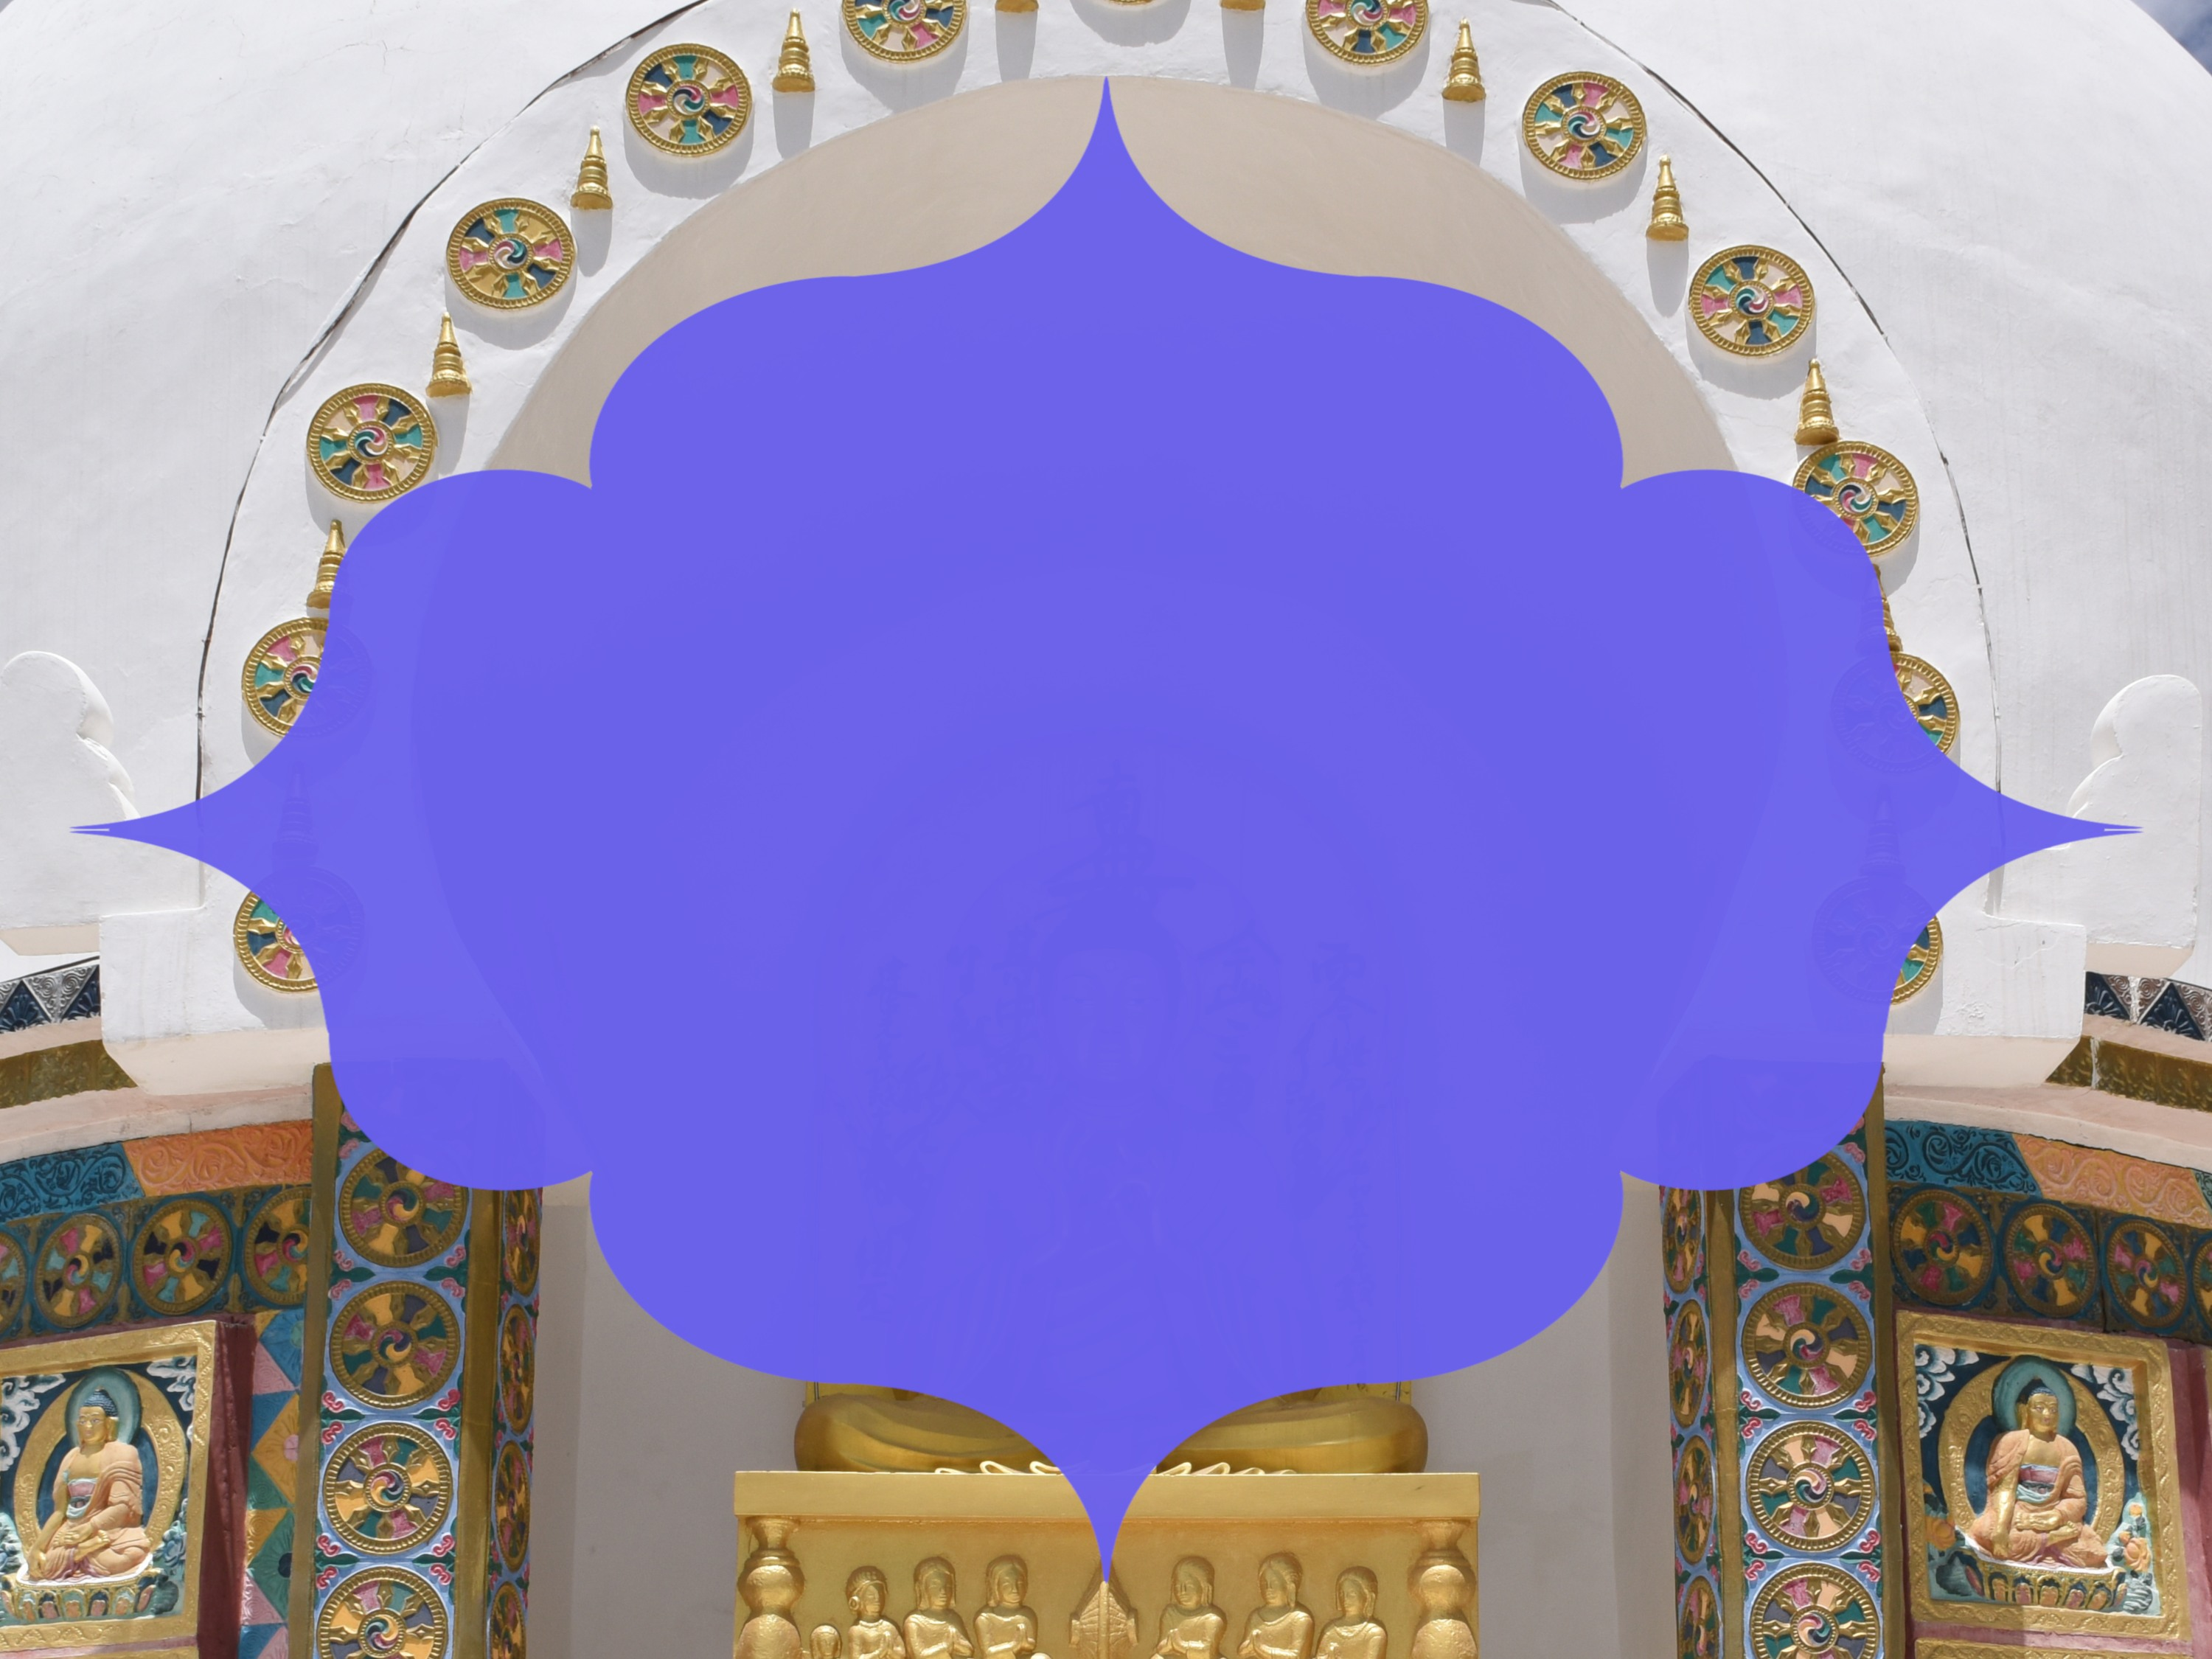
\includegraphics[width=\paperwidth,height=\paperheight]{wheel3.jpeg}}

\begin{titlepage} % Suppresses headers and footers on the title page
	\centering % Centre everything on the title page
	%\scshape % Use small caps for all text on the title page

	%------------------------------------------------
	%	Title
	%------------------------------------------------
	
	\rule{\textwidth}{1.6pt}\vspace*{-\baselineskip}\vspace*{2pt} % Thick horizontal rule
	\rule{\textwidth}{0.4pt} % Thin horizontal rule
	
	\vspace{0.25\baselineskip} % Whitespace above the title
	
	{\scshape \large The Buddhist Praying-Wheel}
	
	\vspace{0.25\baselineskip} % Whitespace above the title

	\rule{\textwidth}{0.4pt}\vspace*{-\baselineskip}\vspace{3.2pt} % Thin horizontal rule
	\rule{\textwidth}{1.6pt} % Thick horizontal rule
	
	\vspace{0.25\baselineskip} % Whitespace after the title block
	
	%------------------------------------------------
	%	Subtitle
	%------------------------------------------------
	
	{\scshape \scriptsize A Collection of Material bearing upon the Symbolism of the Wheel and circular Movements in Custom and Religious Ritual}

    	\vspace*{0.25\baselineskip} % Whitespace under the subtitle

	{\scshape By \normalsize William Simpson} % Subtitle or further description
	
	\vspace*{0.25\baselineskip} % Whitespace under the subtitle
	
    {\scshape\scriptsize R. I., M. R. A. S., F. R. G. S., Hon. Associate R. I. B. A., etc.} % Subtitle or further description
  
    \vspace{0.25\baselineskip}
    
        \begin{quotation}\tiny
`Instruct the planets in what orbs to run,

Correct old Time, and regulate the Sun;

Go soar with Plato to the empyreal sphere,

To the first good, first perfect, and first fair!

Or tread the mazy round his followers trod,

And quitting sense call imitating God;

As Eastern priests in giddy circles run,

And turn their heads to imitate the Sun.'

\begin{center}Pope, \emph{Essay on Man}.\end{center}
        \end{quotation}

  
	%------------------------------------------------
	%	Editor(s)
	%------------------------------------------------

	\vspace{0.25\baselineskip}

	{\scriptsize\scshape London 1896}
	
	{\scriptsize\scshape{Macmillan and Co., Ltd.}}
	
	\vspace{0.25\baselineskip} % Whitespace after the title block

    {\scshape\small Internet Archive Online Edition}  % Publication year
	
	{\scshape\scriptsize Attribution NonCommercial ShareAlike 4.0 International } % Publisher
\end{titlepage}
\setlength{\parskip}{1mm plus1mm minus1mm}
\clearpage
\tableofcontents
\clearpage
\listoffigures
\clearpage
\begin{quotation}\small
`The heavens declare the glory of God; and the firmament sheweth his handywork. Day unto day uttereth speech, and night unto night sheweth knowledge. There is no speech nor language, where their voice is not heard. Their line is gone out through all the earth, and their words to the end of the world. In them hath he set a tabernacle for the sun, which is as a bridegroom coming out of his chamber, and rejoiceth as a strong man to run a race. His going forth is from the end of the heaven, and his circuit unto the ends of it.' --- Ps. 19.
\end{quotation}

\bigskip
\centerline{\EightStarTaper}
\centerline{\EightStarTaper\EightStarTaper}
\bigskip
\clearpage
\begin{quotation}\small
`That day, as other solemn days, they spent

In song and dance about the sacred hill;

Mystical dance, which yonder starry sphere

Of planets, and of fixed in all her wheels

Resembles nearest, mazes intricate,

Eccentric, intervolved, yet regular,

Then most, when most irregular they seem;

And in their motions harmony divine.'

\hspace*{35mm}\emph{Paradise Lost}, Bk. 5.
\end{quotation}

\bigskip

\begin{quotation}\small
\hspace*{25mm}`He, who hath the power, 

Had with another sun bedecked the sky.

Her eyes fast fixed on the eternal wheels

Beatrice stood unmoved.'

\hspace*{35mm}Dante, \emph{Par.} Canto 1.
\end{quotation}

\bigskip

\begin{quotation}\small
`Weave a circle round him thrice,

And close your eyes with holy dread,

For he on honey dew hath fed,

And drank the milk of paradise.'

\hspace*{35mm}Coleridge, \emph{Kubla Khan}.
\end{quotation}
\clearpage
\begin{quotation}\small
\emph{Athenian Stranger}... the soul then directs all things in heaven, and earth, and sea by her movements... If, my friend, we say that the whole path and movement of heaven, and of all that is therein, is by nature akin to the movement and revolution and calculation of mind, and proceeds by kindred laws, then, as is plain, we must say that the best soul takes care of the world and guides it along the good path.

\emph{Cleinias.} True.

\emph{Ath.} But if the world moves wildly and irregularly, then the evil soul guides it... Of these two kinds of motion, that which moves in one place must move about a centre like globes made in a lathe, and is most entirely akin and similar to the circular movement of mind.

\emph{Cle.} What do you mean?

\emph{Ath.} In saying that both mind and the motion which is in one place move in the same and like manner, in and about the same, and in relation to the same, and according to one proportion and order, and are like the motion of a globe, we have invented a fair image, which does no discredit to our ingenuity.

\emph{Cle.} It does us great credit.

\emph{Ath.} And the motion of the other sort which is not after the same manner, nor in the same, nor about the same, nor in relation to the same, nor in one place, nor in order, nor according to any rule or proportion, may be said to be akin to senselessness and folly.

\emph{Cle.} That is most true.

\emph{Ath.} Then, after what has been said, there is no difficulty in distinctly stating that since soul carries all things round, either the best soul or the contrary must of necessity carry round and order and arrange the revolution of the heaven.

\emph{Cle.} And judging by what has been said, Stranger, there would be impiety in asserting that any but the most perfect soul or souls carries round the heavens.

\bigskip

\hspace*{45mm}Plato, \emph{Laws}, Jowett's translation, 10. 897.
\end{quotation}

\bigskip
\centerline{\EightStarTaper}
\centerline{\EightStarTaper\EightStarTaper}
\bigskip
\vspace*{\fill}
\clearpage
\vspace*{\fill}
\begin{figure}[H]
\centering
\includegraphics[width=0.63\textwidth,keepaspectratio]{figs-trans-white/frontispiece.png}
\caption[Frontispiece.]{\bfseries Frontispiece.}
\end{figure}
\vspace*{\fill}
\clearpage
\large
\section*{Introductory}
\paragraph{}
The Buddhist ``Praying-Wheel'' --- the name by which this instrument of worship is known --- has been looked upon by most writers as a strange freak of superstition, and as being quite exceptional as a form of ritualism. Carlyle, with an air of contempt, defined it as the ``Rotatory Calabash.'' Travellers have generally talked of the grinding of prayers in a mill as a good subject for jokes. No one appears to have applied himself to study or comprehend this particular form of worship, so very little seems to be known about it. It so chanced that I spent the hot seasons of 1860 and 1861 in the Himalayas, and in both years I passed over the boundary into Tibet, visited the Lamaseries, and made sketches of the so-called Praying-Wheels. I also bought one of the small hand-cylinders, and learned the proper manner of using it. On my return home I gave some attention to the subject, and discovered that the name ``Praying-Wheel'' was a misnomer; and my investigations led me to the conclusion that the circular movement was symbolical of the solar motion, --- or it might be of the great celestial rotation as it appears above. This result completely changed the whole aspect of the subject. I also saw the similarity of the circular movement of the wheel with circular movements in ritual and custom in India and other parts of the world, and particularly with the Celtic \emph{deisul}. I was then led to write an article on the subject, which appeared in \emph{Good Words} for December 1867; and, so far as my knowledge goes, this was the first effort that had been made to work out the meaning of the Praying-Wheel, and its conclusions have now been fully confirmed.

Since then, in travelling and in reading, I have made notes of whatever seemed to be related to this subject, and the following pages are the result. No pretence shall be assumed on my part that this is an exhaustive treatment; on the contrary, it must be understood that the matter given here is only what I have chanced to come upon. There are many blanks that have yet to be filled in, and I have no doubt that others will accomplish this, who may take up the subject in the future. This, I feel sure, will be done, because the circular movements are intimately related to many questions in comparative mythology; and they are also closely connected with the field of inquiry to which the students of Folk-Lore are directing their attention. My own hope is that what is here given will be found to be at least an interesting chapter in the history and development of one form of ritualism and custom.

My acknowledgments are due to many friends for kindly assistance in this work. My thanks are specially owing to M. Henri Gaidoz, Directeur à l'École des Hautes Études in Paris. His work, \emph{Le Dieu Gaulois du Soleil, et le Symbolisme de la Roue}, treats most ably on one branch of the subject in which my opportunities of acquiring knowledge have been of the slightest; and I am indebted to him for permission to make any use of the valuable information his book contains, and also for the advantage of copying some of his illustrations, which it will be found I have freely availed myself of. I can recommend the production of M. Gaidoz to those who wish to study the particulars of the subject more fully, because he has dealt in a much more complete manner with the symbolism of the wheel in Western Europe than I have done. I may at the same time express my satisfaction in finding an ally in this savant, who has arrived independently at conclusions so similar to my own upon the solar symbolism of the wheel. I also owe thanks to Miss Gordon Cumming, who placed some of her drawings at my disposal. This lady, it ought to be mentioned, has in her travels collected a large amount of information on the wheel and its symbolism. Professor Rhys Davids, from whom I have taken several extracts, has aided me with his counsel and help in some Sanskrit words; and has also most kindly read over and corrected the proofs of the Buddhist and Brahmanical portions of these pages, which is in itself a guarantee that that portion of the work is not likely to contain any very serious blunder in it. Dr. A. S. Murray and Dr. Budge of the British Museum have also assisted me by answering questions and supplying information. Robert Brown junior was at considerable trouble in writing to me about the Greek Chorus, --- on which I have not ventured to say much, as it would require one better informed on the matter than myself. This is one of the blanks that has yet to be filled in, --- to which I would also add dancing in general. The Rev. Dr. A. Löwy, with his almost inexhaustible stores of knowledge of his own people, has been most kind in giving me information about the Jews. Dr. Chaplain was so obliging as to write to Jerusalem to one of his many friends there about some details; and the answer, written I think by a Jew, is given in the Additional Notes. I am indebted to the Rev. Richard Conway for his valuable assistance in relation to the rites of the Latin Church.

I have many friends to thank that I have troubled with questions; the curious thing being --- what I have found in my own case --- how uncertain after years, in some instances even months, the mind becomes about small details. My questions have generally been about the particular direction of turning movements, and the difficulty has been for the memory to recall with certainty how the movement took place. If errors of fact on points such as these should chance to have crept in to what I have recorded, I can only assure the reader it has been from no absence of desire on my part to be accurate.

It was only when the sheets of this work were going through the press that a friend called my attention to the passage from Plato which fronts the beginning of this Introduction. The words are placed there, because on reading them I felt as if they had been the text which I had been expounding. Let those who chance to read the following pages turn back afterwards to what the great Philosopher has said, and they will then understand how appropriate the passage really is, and how completely he had grasped the theory of the wheel and its symbolism as they have been described in this book.
\clearpage
\section{Chapter 1. --- Among the Lamas}
\paragraph{}
In the summer of 1860 being at Simla, I, with a friend, started for Chini, a village in the Sutlej valley, about sixteen marches inland among the hills. The attractions of this place were the fine view of the snowy range, and the escape from the rains, which are usually very heavy at Simla in June and August. We remained two months at Chini, and became intimately acquainted with the people. They are of the Aryan type, but polyandry is a custom among them, and their religious rites can scarcely be classed as Brahmanical. Caste does not exist, and everything is rude and primitive in the extreme. We learned that just across the range of hills that formed the watershed on the right bank of the Sutlej, the people there are known as \emph{Bot log}, or Tibetans; this means that they are Turanian, or Mongolian, in type; and that among them we should find Lamas and nuns, and see their monasteries, Praying-Wheels, and whatever belonged to their peculiar system. An excursion of a few days enabled us to see the villages of Leepee and Kanum; and luckily we found in these places all that we expected. For a couple of rupees I was able to buy a small hand Praying-Wheel (Fig. 1), and the Lama initiated me into the proper way of turning it, and the right use of the \emph{Mantra} during the performance. This was my first contact with Buddhism, and the beginning of my knowledge of the Dharma-Chakra, or Praying-Wheel.

\begin{figure}[H]
\centering
\includegraphics[height=0.3\textheight,keepaspectratio]{figs-trans-white/fig001.png}
\caption[Fig. 1. --- Small hand Praying-Wheel.]{\bfseries Fig. 1. --- Small hand Praying-Wheel.}
\end{figure}
\paragraph{}
I spent next summer in the Himalayas, and arranged to pass through that part of Tibet known as Ladak, going over the high passes to the Indus, and returning by way of Kashmir. Starting from Mussoorie I went to the sources of the Ganges and the Jumna; then crossed over the Roopin Pass, --- which is 15,000 feet above the sea, --- into the Buspa Valley, crossed the Sutlej near Chini, and went on to Leepee, where I had been the previous season; the route led through Kanum, and on to Soonum.

As I entered the village, my ear caught the sound of a bell tinkling at regular intervals; there was some difficulty in climbing up to a window, through which I had an obscure glimpse of a large cylinder and a solitary monk sitting turning it, every turn causing the bell to sound. The place was a monastery, and I had some trouble in finding my way in, but at last I gained admittance, and made a sketch of the room, including the cylinder and the monk. The cylinder might be about nine feet in height and four feet in diameter, with an iron spindle at each end; on the lower one there was a crank to which a string was attached, and by simply pulling this the machine went slowly round. It was gaudily painted with many bright colours, in which ornaments and Tibetan letters formed the designs; the walls of the room were also decorated with paintings of Buddhist figures (see Frontispiece). In addition to these there was a large figure modelled in plaster and painted with many colours, the name of which I learned was Tchaypungmay. A piece of red cloth, the same as the Lamas wear, was hung over its shoulders, partly like a robe and partly like a shawl. The monk who was turning the wheel wore the usual red dress of the Lamas in that locality, yellow being the colour in other parts of Tibet. Yellow is the colour worn in Ceylon and China, and it was the colour in India. The old accounts of converting new regions to Buddhism describe the success of the missionaries by saying that ``the land glittered with the yellow robes.'' The followers of the Dalai-Lama and the Tashi-Lama wear the yellow dress, which is distinctive of the sect known as Gelukpas; while the red dress is the costume of the Dukpas, and their spiritual head is the Dharma Rajah.

The Lama who was moving the wheel did not seem to be annoyed at my rather unceremonious entrance; on the contrary, he appeared to be pleased at his operations being taken notice of. It so chanced that I had some coins in my pocket, and on presenting him with some of these his delight seemed to be great. Native coins are, or were at that time, rough, unshapely pieces of copper very rudely stamped. Those I had given him were the ``Coompany-ke-pice,'' from the Government mint, and they had the Queen's head on them as perfect as on our money at home. As the man, in that out-of-the-way spot, had perhaps never seen such objects before, he gazed with an expression of surprise and wonder upon them, and my guess at the moment was that he took the head of Her Majesty for a Devi, or goddess. So deep was his interest, he forgot to keep the ``Precious Wheel of the Law'' in motion. After a close inspection he wrapped them up carefully in a part of his dress, and commenced to turn the wheel. That did not continue long, for he stopped it again, unrolled the coins to gaze upon them once more. When I left he was sitting looking at them with evident delight. The probability is that the coins would be placed on one of their altars, and that the Queen would become, in that Lamasery at least, a Buddhist deity, and receive suitable adoration. I was led to this conclusion afterwards from what I saw in other temples, where I found that European articles had been picked up by the monks and placed among their figures of gods on their shrines. In one temple I saw two brandy bottles so honoured; and in a monastery at Lamayuru the monks pointed with pride to a gin bottle on their altar, which they seemed to prize highly from the label, which shone in gold and bright colours, and prominent upon it were the figure of a cat and the words ``Old Tom.''

Later in the day I found another temple in the same village with three large cylinders, all of them somewhat similar to the first. On the outside of the temple there was a long row of small cylinders, each about the size of an oyster-barrel; those were placed in the wall at such a height that any one in passing could turn them with the hand. At the monastery of Hemis, near Leh, I saw a similar row of cylinders. It was at Soonum I saw for the first time these cylinders turned by means of water-power. A rude erection had been made over the stream with recesses to hold three barrels; one was empty, the wheel in another was out of order and motionless, but the third went steadily on, revolving day and night. Those cylinders were a little over three feet in height, and the wooden axle was continued downwards, and pieces of wood were fixed to it, producing a horizontal paddle-wheel, and the water dashing on it caused the circular motion. In front was the place where the villagers took their water for domestic purposes, and it is a probable conjecture that it acquired some special virtue from having turned the ``Precious Wheel'' (see Fig. 2).

\begin{figure}[H]
\centering
\includegraphics[width=0.85\textwidth,keepaspectratio]{figs-trans-white/fig002.png}
\caption[Fig. 2. --- Praying-barrels propelled by water-wheels, at Soonum.]{\bfseries Fig. 2. --- Praying-barrels propelled by water-wheels, at Soonum. From a Sketch by the Author.}
\end{figure}
\paragraph{}
It was some marches after that before I chanced to see another of the uses to which the wheel could be applied. We had passed Dunker, and were at the last village before passing the Parung Law, one of the highest passes in the Himalayas, being 19,000 ft. above the sea. The place was named Kiwar; there two men appeared. I assumed they were itinerant Lamas that had come out on a begging trip. They had a small box which held some brass cups, and a small brass figure of \emph{Shakya-Thubba}, as they call Buddha. Those were placed on the top of the box, so as to form a simple altar, and two or three pictures were hung upon the wall behind. One of the men had a mask on his face made of a black coloured cloth, ornamented with cowrie shells. He had a pair of cymbals, which he clashed as he danced before the altar. The other man had a strange head-dress formed of strips of coloured cloth that partly covered his face. He stood by the altar with a small Praying-Wheel in his hand, which he kept turning, and at the same time, in a low monotonous voice, he muttered what I took to be prayers, or the words of some kind of religious service, in which I could often hear the sentence --- ``Aum! Mani Padme, hung!'' This is the \emph{Mantra} of the Praying-Wheel, and will be explained further on. The villagers made offerings in the form of grain, which was laid down in front of the altar.

After crossing the Parung Law we came to the Tchoomoreree Lake, the surface of which is about 15,000 feet above the sea. At this great altitude there were no houses or villages, but at one end of the lake there was, at a place called Korzok, a large Lamasery, with about forty Lamas in it. I made some sketches in that place, and as the use of the wheel there was like what I saw in other monasteries, a description of it will serve for all. These establishments are not remarkable for cleanliness, neither are the Lamas. They have very long services, so tea is served out to them. Tea in Tibet is a very different concoction from what it is in Europe. I have seen it made by our Tibetan [day labourers] in camp. A large pot is put on the fire --- a teapot it may be called, of course, but not in our sense of that word; it was a large iron pot, such as soup would be prepared in. In this tea is made, with butter or grease of some kind, and a few vegetables are added, if they can be procured, so that it is in reality a kind of thin soup. Each man in this region carries a small wooden bowl, somewhere in his bosom --- that is, between his dress and his skin --- and this vessel is brought out whenever tea has to be taken. At the Korzok monastery I had a serious trial to undergo that had not been calculated upon. The Lamas were at their service, which was a long one, and a younger brother came round with a supply of tea for them. As I was sitting sketching among them they wished to be polite, and one of the cups was produced, most probably from its usual receptacle, and some of the tea was poured into it for me. These Lamas had been so kind and genial in every way, I felt it would have been very bad manners to have refused the offered beverage. All the details given above were perfectly well known to me, and to accept the bowl and put it to my lips required some resolution, but I did it, and managed to look pleased after accomplishing it.

\begin{figure}[H]
\centering
\includegraphics[height=0.4\textheight,keepaspectratio]{figs-trans-white/fig003.png}
\caption[Fig. 3. --- Dorjé, or Vajra.]{\bfseries Fig. 3. --- Dorjé, or Vajra.}
\end{figure}
\paragraph{}
The temple in most of these Lamaseries has a recess or apse at one end, in which is placed a figure of Shakya-Thubba, or Buddha, or of some Bodhisatva; and a large opening in the roof allows the principal light of the place to fall upon it and the altar, which stands in front. The Lamas sit in two lines, one on each side of the building. Each Lama has a small desk or stool, on which the books with the service are placed. They have drums, cymbals, and long trumpets. These last are of brass, and very long, as much as seven or eight feet in length. They rest on two low stands, the mouthpiece being close to the Lama that uses it; and at the part of the service when its music is required he lifts the one end only and performs. The service is in printed books, which are in form like those of Ceylon --- that is, the leaves are a series of long strips, enclosed within two boards and tied with a string. In Ceylon the leaves are the dried leaves of a plant, and books are written; whereas in Tibet paper is in use, and books are printed --- from blocks, I presume, as in China. There are three highly-ritualistic instruments which are used by the Lamas. At this time, so long after my visit among them, I do not feel sure whether every monk had them, or if it was only some of those that may have held higher rank. The first of these is a small hand-bell; these are of brass, and ornamented with Buddhist symbols. What signification they attached to this article I did not learn. It is not peculiar to the Buddhists; almost every Hindu temple has one. They are carved on Hindu architecture, and the Bull, Nandi, the \emph{wahan} of Siva, is always represented with one hanging by a cord or chain round his neck. It is a very ancient symbol, but I have never as yet heard any suggestion as to its origin or meaning. The Lamas call it \emph{Drilbu},\footnote{\emph{Dril-bu}, a ``little bell,'' Cunningham's \emph{Ladak}, p. 373.} and it is rung repeatedly at different parts of the service. The second article is called in Tibetan a \emph{Dorjé}, and has been described as a ``sceptre'' (see Fig. 3). It is understood to be the same as the \emph{vajra}, or ``thunderbolt,'' of the Brahmans, which is the \emph{trisula}, or trident, and is the sceptre of Siva, --- temples of Siva have the trident placed upon the \emph{sikhara} or spire.\footnote{The \emph{Trisūla}, or Trident, is a very ancient symbol, and appears to have been known in most parts of the Eastern world. There are also symbols which bear a strong resemblance to it, such as the \emph{fleur-de-lis}, which is supposed to have been brought from the East. A considerable collection of these forms will be found in a paper on the ``Trisula Symbol,'' which I read to the Royal Asiatic Society, and published in the \emph{Journal} for 1890, p. 299.} The Tibetan \emph{Dorjé} does not at first sight suggest any resemblance to the trident, but it is in reality a group of two or four tridents combined, and as the outer prongs come round and meet at the point of the central one, the whole has somewhat the appearance of a crown. That this is a correct explanation, I have a sufficient evidence in possessing a Buddhist \emph{Dorjé} in which the prongs are not repeated, and it is simply a trident. Both ends of the instrument, which is about six inches long, and made of brass, have the prongs, and the space between is the handle by which it is held, which is done repeatedly during the service. What those Lamas understood as the meaning of holding this sceptre in their hands at particular times my want of the language prevented me from learning. The connection of the wheel and the thunderbolt is a very curious one, and as it is found in other places, it will be often referred to again in these pages.

The third ritualistic instrument is what I have, in the meantime, called the ``Praying-Wheel''; and the description of which will be given further on. It lay on the desk before the Lama, along with the \emph{Drilbu} and \emph{Dorjé}, and was at times taken up and whirled round. I often noticed that while the Wheel was turned in the right hand, the \emph{Dorjé} was held in the left. Sometimes none of the three articles would be used, but they would lie on the desk for some time. Not being able to follow the service, it was impossible for me to understand why or when the performance with them was necessary. So far it may be explained that, according to the Buddhist doctrine of \emph{Karma}, or good works, the more a wheel is turned, the more \emph{Karma}, or merit, is acquired by the person who causes it to turn; and from this it may be assumed that in the case of the cylinders propelled by water-wheels, the constant turning would add to the merit of those connected with their erection. The doctrine of \emph{Karma}, which is so prominent in Buddhist teaching, thus explains the motive in the mind of the person turning the wheel, but the symbolism belonging to it is a separate matter, and has yet to be dealt with.

\begin{figure}[H]
\centering
\includegraphics[width=0.85\textwidth,keepaspectratio]{figs-trans-white/fig004.png}
\caption[Fig. 4. --- Praying-Barrels at Kalsi, on the Indus.]{\bfseries Fig. 4. --- Praying-Barrels at Kalsi, on the Indus. From a Sketch by the Author.}
\end{figure}
\paragraph{}
The villagers in some instances use the wheel. This I know from a man who at one place came to my camp, and while I sketched him he sat turning his hand-cylinder. As this was the only one I saw, my impression is that few of the laity --- if that is the right term to apply to the non-Lama part of the population --- are in the habit of using the small hand ones, but then there are larger ones erected in many cases for what may be supposed to be public use. In the village of Kalsi, on the Indus, there was a \emph{Chhod-Ten} --- the Tibetan form of the Indian stûpa --- in the base of which there were two cylinders, about three or four feet in height; those were for the villagers to turn with their hands when they chanced to pass (see Fig. 4). The row of small barrels at Soonum I have already described; and I saw a similar row in the Hemis monastery, on the Indus, near Leh, which was no doubt intended to be turned by all those that chanced to pass, whether monks or laymen (Fig. 5).

\begin{figure}[H]
\centering
\includegraphics[width=0.85\textwidth,keepaspectratio]{figs-trans-white/fig005.png}
\caption[Fig. 5. --- Praying-wheels in the Hemis Lamasery, on the Indus.]{\bfseries Fig. 5. --- Praying-wheels in the Hemis Lamasery, on the Indus. From a Sketch by the Author.}
\end{figure}
\paragraph{}
The only other place where I saw a wheel turned by water-power was at Ghia (see Fig. 6); that one, by some arrangement, gave a click at every turn. My tent chanced to be near, and on going to bed I could hear it. I fell asleep listening to the click, and it was the first sound I heard again in the morning when I wakened. I add an illustration of another wheel at Ghia, in which I could only see the water-wheel beneath (see Fig. 7). It was not my fortune to see wheels driven by windmills. Huc, if I remember right, mentions them; and Bonvalot, one of the latest travellers in Tibet, saw them.\footnote{\emph{Across Thibet}, by Gabriel Bonvalot, vol. 2. p. 143.} It seems to be a matter of no consequence by what means these cylinders are turned; the \emph{Karma} can be realised if only the circular motion can be produced. In some cases the hot air from fires is thus utilised. Huc says that ``the Tartars suspend them over the fireplace... the movement itself is effected by the thorough draught occasioned by the openings at the top of the tent.''\footnote{\emph{Travels in Tartary, Thibet, and China}, by M. Huc, vol. 1. chap. 9.} To this may be added the statement of the Rev. James Gilmour, a missionary, who spent a good many years among the Mongols. In describing Wu T'ai Shan, a great place of pilgrimage, he visited one of the important Lamas, and in his room, ``near the ceiling, just above the charcoal fire, hung a paper cylinder, like an inverted wheel of life, which kept constantly turning. That was also a praying-wheel, and was kept in motion by the hot air ascending from the fire.''\footnote{\emph{Among the Mongols}, by the Rev. James Gilmour, M. A., p. 147. Gilmour describes a tope at Wu T'ai Shan, and round its base ``were mounted more than three hundred praying-wheels, which the worshippers set in motion one after the other as they passed round, p. 146.} It is evident from these examples that, if smoke-jacks could be introduced into Tibet, they would be highly prized in every household as a means of acquiring \emph{Karma}.

\begin{figure}[H]
\centering
\includegraphics[width=0.85\textwidth,keepaspectratio]{figs-trans-white/fig006.png}
\caption[Fig. 6. --- Praying-Barrel at Ghia.]{\bfseries Fig. 6. --- Praying-Barrel at Ghia. From a Sketch by the Author.}
\end{figure}
\paragraph{}
In February 1894, Mr. W. Woodville Rockhill gave an account of his travels through Tibet to the Royal Geographical Society. In describing some Tibetans near Kokonor, he says: ``... The family sleep on a Chinese \emph{kang}, or stone bed, headed by a big Tibetan cooking-stove where the tea-cauldron boils, and over which is a prayer-wheel turning in the heated air as it escapes through a big hole in the roof.''\footnote{\emph{The Geographical Journal}, May 1894, p. 363.} And further he adds, --- ``And below the house, in a log hutch built over the brook, a big prayer-barrel is kept turning ever by the water as it dashes by.''\footnote{\emph{Ibid.}}

\begin{figure}[H]
\centering
\includegraphics[width=0.85\textwidth,keepaspectratio]{figs-trans-white/fig007.png}
\caption[Fig. 7. --- Praying-Wheel at Ghia.]{\bfseries Fig. 7. --- Praying-Wheel at Ghia. From a Sketch by the Author.}
\end{figure}
\paragraph{}
Another peculiar form of this ritualistic machine is a very large cylinder filled with books --- books of prayer, or religious works, we may suppose. These wheels are in temples, and visitors turn them as a religious performance. Miss Gordon Cumming saw and sketched some of these in Japan. That lady calls them ``Scripture-Wheels,'' --- ``circulating libraries'' might be suggested as a good name for them, --- and describes a very striking one she saw in the Asakusa temple at Tokio\footnote{The description and sketches of these Scripture-Wheels appeared in \emph{Scribner's Monthly}, September 1881, p. 733.} (see Fig. 20). Mr. Gilmour saw one at Wu T'ai Shan, which he states was ``about sixty feet high, containing shrines, images, books, and prayers.'' This one was so large, and had such a weight in it to move, that ``two or three together go down to the cellar, lay hold on the hand-spokes, and with a long pull, a strong pull, and a pull all together, round goes the wheel.''\footnote{\emph{Among the Mongols}, p. 146.} According to his account, those who turn this ponderous cylinder believe that they acquire as much merit by the act as if they read all the books, repeated the prayers, and knocked their heads on the ground before all the gods whose images are enshrined in the wheel. Mr. Gilmour is probably quite right in thus describing the thoughts of those who go through such performances; but Dr. Edkins gives an explanation of these ponderous Scripture-Wheels, which is much more in keeping with the original Buddhist ideas on the subject. He quotes a Chinese phrase --- ``\emph{Fa-lun-ch'ang-chwen}, `The Wheel of the Law constantly revolves.' This refers to the unceasing proclamation by books and monks of the doctrines of Shakyamuni. The metaphor by which Buddhist preaching is called the revolving of the wheel is seen practically exemplified in the Praying-wheels of Mongolia, by the turning of which an accumulation of merit is obtained. So in China, the whole Buddhist library of several thousand volumes is placed in a large octagonal revolving bookcase, which is pushed round at the instance of the visitor.''\footnote{\emph{Chinese Buddhism}, by the Rev. Joseph Edkins, D. D., p. 266.} Dr. Edkins also mentions the great wheel at Wu T'ai Shan: ``The Chinese copy of the Gangur is inside it. The visitor sees the whole vast Wheel turning slowly from east to west. All praying-wheels turn in the direction in which the sun moves.''\footnote{\emph{Religion in China}, Edkins, p. 238. Dr. Edkins also mentions a similar Wheel at the Yung-ho-Kung in Peking; and that there was another in the Ling-yin monastery at Hangchow before the time of the Taiping rebellion.} The subject of this last sentence forms an important principle in connection with the wheel, which will be dealt with as we proceed.

Gerard mentions that in the monastery of Soongnum, --- Soonum, where I sketched the large Praying-Wheel, but unfortunately I did not chance to see the one Gerard describes --- there is at that place a library of books, procured from Lhása at a cost of 500 rupees. ``At stated periods the Gelongs and Lamas assemble to read them; and on grand days there is exhibited an iron stand of five squares, one above the other, tapering to the top, which is illuminated with one hundred and eight lamps, and is made to revolve in the same direction as the cylinders.'' This description is not very definite, but it may be assumed that he means the books are placed on the stand and revolve with it.

It will convey some idea of the extent to which these Wheels are in use if we quote again from Mr. Gilmour's interesting book a description he gives of them on his visit to Urga in Mongolia. ``In these temple premises, and at many street corners and busy places, are erected numerous Praying-Wheels, supposed to be filled inside, many of them decorated outside, and some of them almost literally covered all round, with prayers, the idea being that any devout believer who turns the wheel, by so doing acquires as much merit as if he or she had repeated all the prayers thus set in motion. These praying-cylinders seem to be seldom left at rest. In the quiet deserted-looking precincts of the temple may be heard the creaking of the rusty spindle, as it is turned in the unoiled socket by worshippers, who most likely have come from the country to perform their devotions at this great religious centre. Many, both Lamas and laymen, male and female, as they pass along the streets, lay hold of the inviting handle and give a turn to such praying-machines as they find standing in their path.''\footnote{\emph{Among the Mongols}, pp. 134, 135.}

The following is from Bonvalot's book; it refers to a monastery towards the south-eastern border of Tibet, thus showing how widespread the Praying-Wheel is in that region:--- ``The principal attraction of the Dotou-Lama house is a series of prayer-mills. Beneath a gallery running almost entirely round the house are enormous bobbins composed of printed prayers, and transfixed by a long piece of wood, which is held in position by two beams. These bobbins are turned by hand, and as it is said that each is composed of 10,000 prayers, and as there are at least 100 of them, it is easy to see what an enormous quantity of prayers can be said in a walk round the building.''\footnote{\emph{Across Thibet}, by Gabriel Bonvalot, vol. 2. p. 170.} This writer made a wonderful journey across Tibet, but it is evident that he had not paid much attention to the construction or character of the ``praying-mills.'' This description agrees perfectly with the rows of cylinders I saw at Soonum and at the Hemis monastery near Leh.

The small hand-wheels are made of brass. The one in my possession, of which an illustration is given (Fig. 1), is three inches long, and two and a half in diameter. I believe that the high functionaries in the Lama priesthood have them made of gold, and set round with precious stones. Many have the sacred Mantra engraved in Tibetan characters round the outside. My one chances to be without this. By means of a bit of leather and a link, two small bits of lead are attached to the outer periphery of the cylinder, and it is their weight that carries the whole round, which is done by a gentle motion of the hand. The one I have, although very rudely made, when the proper turn of the hand is given, revolves easily and smoothly. Along with the pieces of lead there is a sharp iron hook, by means of which, when the instrument is not in use, it can be hung on to the dress of the performer, where it can be readily caught again and twirled when a spare moment or two occurs. There is a small bell attached to the handle of this particular wheel, which, I think, is not generally the case with others that I have seen. Its purpose I do not know; it does tinkle at times when the cylinder is whirled. The large cylinder I saw at Soonum tinkled a bell at every turn. I have mentioned the bell as one of the prominent ritualistic articles in the Lama service. To this it may be added that the bell occupies an important position in Hindu worship, but its origin and purpose, so far as I can recollect, I never heard explained. There is one theory that is well enough known: it is, that, when the Hindu rings a bell at a temple, he does it to waken the god, so that he may be aware of the worship that is to be offered. This cannot possibly be the meaning of the bell. It may be added that the tinkling of a bell is not limited to the forms of Brahmanical or Buddhist worship.

Here I have given an account of the various forms of the wheel which I have chanced to see in my travels; descriptions have been added of other forms which did not come under my own observation.
\clearpage
\section{Chapter 2. --- The Precious Wheel}
\paragraph{}
I have employed the term ``Praying-Wheel,'' --- and as it has become so well established, I may use the phrase still, --- but one of the purposes of this chapter will be to show that this does not convey a correct idea of the wheel. A marked distinction is at all times made between ``praise'' and ``prayer''; and ``Praising-Wheel'' would be a title that comes much nearer to the true meaning. Although this name expresses to a certain extent the character of the wheel among the Lamas, still it is very far from conveying all the symbolism that belongs to it; but this will be better understood as we advance.

When travelling in Tibet, I understood from the Lamas that they called the wheel a \emph{Mani}; but Cunningham,\footnote{The late Sir Alexander Cunningham, son of Allan Cunningham the Poet. His work on \emph{Ladak} was published in 1854, when he was a brevet-major of Engineers. It is a book full of valuable details. Sir Alexander's service in India was, almost the whole of it, devoted to archæology. He was for many years the head of the Archæological Survey Department. His numerous books on the archæology of India, including the \emph{Archæological Reports}, contain a vast mine of knowledge. He died in December 1893.} who had better means of gaining correct information than I chanced to have, calls them \emph{mani-chhos-khor}, which he translates ``The Precious Religious Wheel.'' This must be a free translation, for \emph{mani} means a ``jewel'' or ``gem.'' \emph{Chhos-khor}, I assume, means ``wheel.'' Huc and other writers give this as \emph{Tchu-kor}; and as \emph{Chakar}, a form of \emph{Chakra}, is the ordinary word in Hindustani for ``Wheel,'' I assume that it is a variant of that term. \emph{Dharma-Chakra} is the Sanskrit name, which is usually translated ``Wheel of the Law,'' meaning the Law or Faith of Buddha.\footnote{\emph{Dharma} (Pāli \emph{Dhamma}) has been translated at times as ``law,'' at times by the word ``faith.'' Professor Rhys Davids says it is a word often most difficult to translate, and best rendered by ``truth or righteousness.'' See his explanation at p. 51.} In Buddhist books it has received a great many titles, such as ``Wheel of Life and Death,'' ``Wheel of Transmigration,'' ``Wheel of Time,'' etc. ``The Royal Chariot Wheel of the Truth,'' and ``The Supreme Wheel of the Empire of Truth,'' are from a Pāli Sutta, translated by Professor Rhys Davids.\footnote{\emph{Dhamma-Kakka-Ppavattana-Sutta}, 25. Sacred Books of the East, vol. 11. p. 153.} According to the same authority, \emph{Dhamma-Kakka} is the Pāli form of the name. In Siamese its name is ``Phra Thamma Chak.'' Alabaster explains \emph{Phra} as ``Holy''; \emph{Thamma} as ``Dharma''; and \emph{Chak} as ``Chakra.''\footnote{\emph{The Wheel of the Law}, p. 169.}

The real character of this symbolical instrument,--- I speak here of the Praying-Wheel as it is understood in Tibet, --- may be realised from the Mantra, which has been so often misrepresented as a prayer. A ``Mantra'' is a word common to both Brahmanism and Buddhism. It means any word, or combination of words, which may be used by way of invocation during an act of worship. For instance, ``Halleluiah'' and ``Hosanna'' would be classed by a Brahman as Mantras. The first chapter of the Koran or the Lord's Prayer would also be included. Any combination of words that may be regularly used for invocation or consecration, or terms used to produce magical results, would be considered Mantras, such as ``Abracadabra,'' or ``Hi! Presto! Fly, Jack, and begone!''

According to my information, the Praying-wheels, whatever may be their size, are filled with paper or cloth, on which is repeated, as many times as it can be written, a Mantra of the following words: ``Aum! Mani Padme, hung!''\footnote{Waddell, in his \emph{Buddhism of Tibet}, p. 139, gives the last word of the Mantra as ``hum.''}

The first word in this sentence is the \emph{Aum} or \emph{Om}, which is so sacred among the Hindus that some will only repeat it without sound, and others only think of it. In the present case it may be understood in the sense of ``Adoration,'' or ``Reverence.'' \emph{Mani} means a ``Jewel'' or ``Gem.'' \emph{Padme} is ``in the Lotus''; and \emph{hung} is usually rendered by ``Amen.'' The whole sentence would thus be, ``Adoration to the Jewel in the Lotus, Amen!'' The words are meant to be an expression of the highest devotion or reverence; nothing is asked or prayed for, and instead of calling these cylinders by the usual accepted name, they should, on the contrary, be called ``Praising-Machines.''

Before turning these wheels, the performer should repeat the Mantra, else he will derive no merit from it; while he is turning, he may repeat the words as often as possible, and at the end a repetition is necessary, or the whole of the performance will be useless. The wheel should be moved round in the direction that a person would go if he turned round an object with his right hand to the centre.\footnote{As I shall have often in this work to describe the direction of circular movements, I intend to describe the two movements by saying that the one was with the right hand, and the other  with the left hand, to the centre. I adopt this because it appears to me to leave no doubt as to the direction of the motion.} To turn the wheel in the other direction produces an evil result; and, if I mistake not, such a motion is believed to undo any merit that had been previously produced by turning it in the right manner. As I knew nothing of the language while in Tibet, I was unable to ask questions. On that account there are many details about these wheels, concerning which I should have wished to possess more information, but was unable to obtain it on the spot. One point was as to whether this circular motion was in imitation of the sun. I have already quoted from Dr. Edkins, that ``all Praying-Wheels should turn in the direction in which the sun moves.''\footnote{\emph{Religion in China}, p. 238.} Many things in Chinese Buddhism came through Tibet, among these was the Wheel, so we may assume that this was the Tibetan theory regarding its movement.

The Tibetans construct long dikes of stone; Mani is also the name given to these. They vary from about six to twelve feet in width, and are about four or five feet in height, from which they slope upwards to a ridge in the centre, like the roof of a house. The length of these varies from a few feet to that of the very long one at Leh, which Cunningham measured, and found it to be 880 paces, or nearly half a mile.\footnote{\emph{Ladak}, p. 378.} The Lamas engrave on stone slabs the favourite Mantra, ``Aum! Mani Padme, hung!'' repeating the words as often as the size of the slab permits. These the people buy and lay on the sloping top of the Mani, for good luck in any undertaking they may be about to begin. Manis such as these are generally built on the public road, at the outskirts of the village, and anyone passing, does so keeping them on the right hand. By observing this rule, a person going and coming back again is considered to have circumambulated the Mani; and he will have done so with his right hand to the centre, which is the same circular motion as the wheel.\footnote{The following is a Hindu form of circumambulating, which bears a strong resemblance to walking along the Manis. ``A pilgrim, for example, sets out from the source of the Ganges, at Gangotrī, and walks by the left bank of the river to its mouth, at Gangā-Sāgara; then, turning round, he proceeds by the right side back to Gangotrī, whence he departed. This is called Pradakshinā'' (\emph{Hinduism}, by Sir Monier Williams, p. 173). ``Pradakshinā,'' it may be explained, means circumambulating.} This performance of going round sunwise will be seen, as we proceed, to have been one of the world-wide customs; in some places it is only a custom, while in others it is part of a religious observance.

When the Prince of Wales was at Jummu the Maharajah of Kashmir had a party of Lamas brought there, and they performed one of their wild, grotesque, masked dances, which I witnessed at the time. Here is an account of it that appeared in one of the Indian papers, in which it will be seen that the whirling round was done in the same direction as that of the Praying-Wheels. The place was cleared and ``the Lama orchestra came in. It was formed of the musicians who perform in the monasteries, and had four large brazen trumpets, about six or seven feet long, which gave forth a deep sound as if it were the grumble of an earthquake. There were four drums, their shape reminding one of the old traditional warming-pan, held on end, and beaten with a curiously bent drumstick. There were cymbals and other instruments producing a clashing noise. The Lamas with these articles came in and squatted down in a long row like sitting Buddhas, and a wild gust of sound from them ushered in the dancers, who came along jumping and whirling in the most outrageous costumes. One man carried an incense vessel, held in his hands with chains identically as it is carried in a Roman Catholic Church. One man had a hat in colour and shape resembling the comb of a cock, but most of them had huge wide-brimmed hats surmounted by tridents and all sorts of things like vanes and weathercocks, from which long strips of coloured silk hung down behind. The costumes were purely Chinese, the body of their dresses being similar to that worn by Mandarins, only that they had capes, aprons, and tags and rags of all kinds hanging upon them, which flew out as the dancers went round in their uncouth gambols. \emph{After dancing in a circle for a short time, going round with the right shoulder to the centre, which is the same turn as the Praying-Wheel goes round}, they retired and very quickly came back again. The large broad-brimmed hats were wanting, and all the dancers had the heads of animals exactly like what we see in a pantomime; there were ox-heads, boar-heads, elephant-heads, also large grinning and laughing heads, painted in all tints. The jumping and whirling round was the same each time they changed their head-dresses. We were led to understand that symbolism was expressed in the costumes, the heads, and in all the various parts of this uncouth performance, but its meaning was not at all clear to our Western ideas.''\footnote{\emph{The Indian Public Opinion and Panjab Times}, January 1876.}

According to Huc, the Mantra is known to the Tibetans as the ``Mani''; this will explain why the name is given to the Wheel as well as to the dikes of stone. Huc says that this Mantra is not only in every one's mouth, but it is written everywhere. Rich Tibetans employ men to go about with chisel and mallet over the country to engrave it on rocks and stones.\footnote{\emph{Travels in Tartary}, vol. 2. p. 194.} It is called the \emph{Shadakshara Mantra}, or ``Six-Syllabled Charm.'' From what has already been said it is scarcely necessary to repeat that the Mantra is considered to be a most potent sentence. The Lamas, according to Huc, affirm that the doctrine contained in these ``marvellous words is immense''; and the whole life of man is insufficient to realise its complete breadth and depth. Huc consulted the Regent of the Dalai-Lama, who told him that living beings are divided into six classes --- angels, demons, men, quadrupeds, birds, and reptiles; and these six classes correspond to the six syllables of the Mantra. It was by repeating these syllables that men avoided transmigration into the lower animals; and rose up in the scale of being till they were absorbed into the universal soul, or the grand and eternal essence of Buddha.\footnote{\emph{Ibid.} pp. 195, 196.}

The wheel as a ritualistic instrument or ``machine'' appears to be peculiar to Tibet, and Mongolia might perhaps be added. In India the wheel --- as will be shown further on --- was only a symbol; it was in no case an article that could be practically turned with the hands.\footnote{It will be seen further on that this statement is not exactly correct, but I leave it here, and in other instances, as it was written before I discovered in the \emph{Satapatha-Brâhmana}, which will be mentioned further on, that wheels were turned in India before the Buddhist period.} Ceylon, which is still Buddhist, has no such instrument; neither has Burmah. Alabaster, in his \emph{Wheel of the Law}, shows by the title of his book that in Siamese Buddhism the symbol must be a familiar one, but it is not a machine in that country. In China and Japan, so far as the wheel as a turning instrument is known, we may assume that the practice was derived from Tibet. This naturally suggests the curious question as to how the symbol became a machine among the Turanian races of the Himalayas. To this I can give no answer. Its use in Lamaism may perhaps be a survival of some of the Bonpa --- the pre-Buddhist religion of Tibet --- practices. It may be assumed that in the machine form we have only a developed condition of the wheel symbolism; for that, including other circular movements, is undoubtedly of old date, even ``primitive,'' I believe, is a word that might be applied to it. I shall have other wheels --- wheels in motion --- it may be added, to touch upon later on; but it is doubtful as to whether they will help us in the Tibetan problem.

Cunningham writes that ``on the gold coins of Hoërki, or Hushka, the Indo-Scythian prince is generally represented holding the prayer-cylinder in his right hand.''\footnote{\emph{Ladak}, p. 375.} Other authorities have described as a ``sceptre,'' and a ``club,'' the article in the king's hand which is supposed to be a ``praying-cylinder.'' If it is the latter, it would prove the existence of the wheel as a ``machine'' as early as the first or second century \textsc{ce}; and that would be long before Buddhism is said to have reached Tibet. This monarch was an ``Indo-Scythian,'' or a Mongolian, and it would help to prove what has been already stated that it belonged to an old religious system. This would be a valuable point if it could be satisfactorily established, but the evidence of the coins is so very doubtful that it cannot be accepted.

Cunningham makes a statement about the earliest mention of the praying-cylinder, which would be about 400 \textsc{ce}. This he attributes to Fah-Hian,\footnote{\emph{Ladak}, p. 375.} and does so on the authority of a translation by Rémusat; but since that we have the translation of that pilgrim's travels by Professor Beal, who rejects the earlier rendering, and says there is no reference to ``Wheels'' in the original.\footnote{\emph{Travels of Fah-Hian and Sung-Yun}. By Samuel Beal (ed. 1869), p. 17, note.} This is fully confirmed by Professor Legge, who has also translated the book.\footnote{\emph{Fâ-Hien's Record of Buddhist Kingdoms}. Translated by Professor Legge, p. 23.}

If the Wheel, as a machine, did not pass into Tibet from India, it may be assumed that the Mantra did. Of the six syllables that compose it, five of them at least are Sanskrit, or are derived from that language. It belongs to the Mahayana development, which had taken place before Buddhism had reached Tibet. According to Dr. Waddell, in a paper lately read to the Royal Asiatic Society, the Mantra is more especially connected with the worship of Avalokitesvara, of whom the Dalai-Lama is supposed to be an incarnation.\footnote{\emph{Journ. Roy. As. Soc.}, January 1894.}

The origin and growth of the Mahayana, or system of ``The Great Vehicle,'' in Buddhism, have not as yet been fully brought to light. Probably it was only the absorption by Buddhism of the ideas of older systems, a process which has taken place with other religions.

The Mantra of six syllables which is considered by the Lamas to have such a profound meaning may be taken as an illustration of this. In the Buddhist sculptures of India, figures of Buddha do not appear till about the end of the fourth century; after that date they are common. In these Buddha is represented sitting on the \emph{Padmásana}, or Lotus-Throne. The petals of the lotus are carved all-round the edge of the seat on which the figure sits. It is rare to find a statue of Buddha, either sitting or standing, without the lotus being indicated. In some of the smaller rude figures in marble, the petals are often indicated by only a few ogee lines. In large and highly-finished figures, again, the petals are made so ornamental, that their real character might be difficult to realise.\footnote{It may be mentioned that the figures of Brahmanical deities are also often represented as sitting or standing on a \emph{Padmásana}, or Lotus-Throne.} This conventional form of Buddha sitting or standing on this symbolical flower is exactly according to the ``Jewel in the Lotus'' of the Mantra.

Ideas of an abstract kind may be supposed to exist before they find expression in art. In the earlier Buddhist books Buddha appears as little more than a teacher. When he went to the Isipatana deer-park, at Benares, and began to ``turn the Wheel of the Law,'' no such wheel as the Tibetan Lamas turn is supposed to have existed. The expression only meant that Buddha began to teach his doctrine, and ``found the Kingdom of Righteousness.'' Buddhism had then no cosmogony, nor hierarchy of saints or divine beings. Those were added afterwards, and with them came the symbolism of the lotus. At what time the lotus first became a symbol it would be difficult to say; it was probably early, but the symbolism it represents is well enough understood, and can be traced back a long way. In many of the ancient cosmogonies creation is said to have had water as its origin. In the Semitic system it is distinctly affirmed. With the Chaldeans Professor Sayce states that ``in the cosmology of Eridu... the origin of the universe was the watery abyss.''\footnote{\emph{Hibbert Lectures}, p. 143.} In the Brahmanic cosmogony it is as old as the Vedas. In the \emph{Rigveda} the following occurs in the account of creation: ``There was then neither non-entity, nor entity; there was no atmosphere, nor the sky which is above. What enveloped [all]? where, in the receptacle of what [was it hid]? Was it water, the deep abyss? Death was not then, nor immortality; there was no distinction of day or night: That, being One, breathed calmly, in self-dependence; there was nothing different from It [that One] or above It. Darkness existed; originally enveloped in darkness, this universe was undistinguishable water.''\footnote{\emph{Rigveda}, 10. 129, 1.; Muir's \emph{Sanskrit Texts}, vol. 4. p. 4.} In the \emph{Satapatha-Brâhmana} it is written: ``This [universe] was in the beginning waters, only water.''\footnote{\emph{Satapatha-Brâhmana}, 11. 1., 6, 1.; \emph{ibid.} p. 17.} Indian art represents Vishnu floating on the abyss of waters on the great serpent \emph{Sesha}, which is also called \emph{Ananta}, or ``Eternity.'' From the umbilicus of Vishnu issues the stalk of a lotus, and on the flower sits Brahma in the act of creating all things.

I do not know how the Lamas interpret the ``Gem in the Lotus''; it is not likely that they have adopted the comparative method, which is considered in the present day to be the safest in judging of such matters. That mode of investigation leads to the conclusion that the Mantra is a symbolical form of representing the Creative Force in the act of producing all things. The flower floats on the water, and in the Vishnu-on-Sesha pictures Brahma is understood to be creating. In Genesis the Spirit of God is described as moving on the face of the waters at the beginning of all things. The ark floating on the waters of the Deluge is the same symbolism --- the world had been destroyed, and a new creation had to take place. A Psalm says: ``The Lord sitteth upon the flood; yea, the Lord sitteth King for ever.''\footnote{Psalm 29. 10.} The Fish-god of the Chaldeans was probably another type of the same symbolism. Traces of it are also found in the Egyptian system.\footnote{``There can be no controversy about the meaning of Rā. Rā is not only the name of the sun-god, it is the usual word for sun. In other mythologies the sun-god is borne on a chariot or on horseback; in Egypt, his course across the sky is made in a boat. The sky [\emph{Nu}] is accordingly conceived as an expanse of water, of which the Nile is the earthly representative'' (\emph{Hibbert Lecture}, by P. Le Page Renouf, p. 109). Among the hieroglyphic representations on Belzoni's sarcophagus in the Soane Museum, is that of the sun in the solar bark moving through the celestial waters. Wilkinson describes a picture of the dead in Amenti, and says: ``Horus... introduces him to the presence of Osiris, who... sits on his throne in the midst of the waters'' (\emph{Ancient Egyptians}, vol. 2. p. 447).} In \emph{Poseidôn} we have possibly a similar symbolical idea. The visible earth was his part of his father's inheritance, but he is always represented enthroned upon the waters.\footnote{Robert Brown jun., in his small work entitled \emph{Poseidôn}, identifies, or at least shows some connection between, that deity and the fish-god Dagon, as well as Oannes, pp. 101-110.} El-Masudi writes: ``The first thing created, according to a tradition based on the authority of Ibn el-'Abbás and others, was water; upon it was the throne of God.''\footnote{\emph{Meadows of Gold and Mines of Gems}, translated by Sprenger, vol. 1. p. 43. The Qur'an makes the same statement, ``It is he who created the heavens and the earth in six days, and his throne was upon the water'' (chap. 11., Palmer's translation).} These examples will be sufficient to show how widespread this particular form of symbolism must have been at some early period.

There is another signification which I believe is embedded in this mystical Mantra. On realising the meaning of each word in it, and knowing that the lotus had a sexual symbolism, it dawned upon me, very early in my study of this subject, that a sense could be attributed to the Mantra, as well as to the sculptured figures of Buddha on the lotus, that has its counterpart in Brahmanism. The Brahmanical system, it may be explained, by one process, reduces all the powers of nature to two --- these are male and female. The Padma, or Lotus, it is well known, represents the female \emph{Sakti}, or power.\footnote{``The lotus-leaf is the womb'' (\emph{Satapatha-Brâhmana}, 6. 4, 1., 7, Sacred Books of the East, vol. 41. p. 215).} The jewel, or gem, when joined to it, would represent the male power; and the combination becomes identical with the symbols under which Maha Deo, or Siva, is worshipped. This agrees perfectly with the previous conclusion, as it presents to us the symbolisation of the Creative Power which floats on the water.

I find that this conclusion has been fully confirmed by no less an authority than Sir Monier Williams. In his Lectures on Buddhism, delivered at Edinburgh in 1888, regarding the Praying-Wheel, and the sacred Mantra it contains, he says: ``Doubtless the prayer really owes its origin to the close connection which sprang up between northern Buddhism and Saivism. The worshippers of Siva have always used similar mystical sentences and syllables called Dhâranîs, to which a kind of miraculous efficacy is attributed. In all probability an occult meaning underlies the ``Jewel-lotus'' formula, and my own belief is that the majority of those who repeat it are ignorantly doing homage to the self-generative power supposed to inhere in the universe --- a power pointed at by the popular Sânkhya theory of the union of Prakriti and Purusha, and by the universal worship of the Linga and Yoni throughout India.'' To this a footnote is added: ``I had formed this opinion long before I saw the same view hinted at in one of Koeppen's notes. (See my \emph{Brahminism and Hinduism}, p. 33.) It is certainly remarkable that the name Mani is applied to the male organ, and the female is compared to a Lotus-blossom, in the Kâma-Sâstras. I fully believe the formula to have a phallic meaning, because Tibetan Buddhism is undoubtedly connected with Saivism.''

Some notion may be now formed why this celebrated six-syllabled sentence is so mystical, and is, at the same time, believed to be so potent.
\clearpage
\section{Chapter 3. --- The Wheel in Indian Buddhism}
\paragraph{}
It has been already stated that in Indian Buddhism the wheel was not what might be called a ``machine,'' that is an instrument to which motion could be given by the hand or otherwise, as in Tibet. Its character in Indian Buddhism is that of a symbol. It is often referred to in Buddhist books; and it is of frequent occurrence in Buddhist sculpture. It is also represented on old coins. At Sânchi the wheel was placed in the highest position over the centre of the gateways, --- the fragment of one still remains on the northern gate to show that this was the case, --- thus giving it the most important place amongst Buddhist symbols. Cunningham found that it occupied a similar position at Bharhut. Among the Sânchi sculptures it is seen in a variety of forms. Sometimes on the top of a pillar (Fig. 8); at others it is supported on a pedestal, and figures, including Kinnaras,\footnote{``\emph{Kinnaras}'' are a kind of celestial beings, ``Divine Musicians''; they are variously represented. On the Sânchi Stûpa they have human heads and arms, with what may be intended for the tail and legs of a peacock.} are represented worshipping the wheel, and making offerings to it (Fig. 9). It is frequently combined with the trisūla\footnote{\emph{Trisūla}: this is a form of the trident, a symbol common to both Buddhism and Brahmanism. See \emph{supra}, what has already been stated  regarding the Tibetan ``Dorjé.''} symbol. At Sânchi, and also in the sculptures at Amarávati, the wheel is the principal symbol on the feet of Buddha; in the earlier Buddhist sculptures Buddha himself is not represented. At Amarávati an empty chair is shown, with the marks of Buddha's feet on the footstool below, and the wheel indicated upon each of them (Fig. 10). In the Siamese footprints of Buddha, called the ``Phrabat,'' on which there are 108 symbols, the wheel occupies a large and prominent space in the centre.\footnote{A large and careful illustration of one of these is given in Alabaster's \emph{Wheel of the Law}, p. 286. The author gives a long explanation of it, which will show how important the foot and its symbols were to the Buddhists. One may be seen in the British Museum.} The ``thousand-ray'd Wheel'' on the soles of the feet is one of the marks on a child when born, indicating that he will either be a Chakravarti Rajah, or a Perfect Buddha; and, according to the Buddhist records, Buddha had these marks on his feet at his birth (Fig. 11). As soon as he entered this world, he walked seven steps to each of the cardinal points, and a lotus flower grew up at every step. I note this here on account of the probable connection between the steps and the wheel.

\begin{figure}[H]
\centering
\includegraphics[height=0.5\textheight,keepaspectratio]{figs-trans-white/fig008.png}
\caption[Fig. 8. --- Wheel on Pillar.]{\bfseries Fig. 8. --- Wheel on Pillar. Sculpture at Sânchi. From Cunningham's \emph{Bhilsa Topes}.}
\end{figure}
\paragraph{}
It is often a difficult task to explain old symbols that have come down to us from the past. In many cases we have the symbol, but no descriptive authority for the particular meaning that was attached to it. We know that symbols have had new meanings given to them, and at times the sense in which they were understood has been almost completely changed; this has to be remembered, because although we may know the symbolical interpretation that belonged to one system, or to some particular date, it may not be the same that is accepted when the symbol has been adopted by another system, or at another period of time. The study of symbolism is on this account surrounded with difficulties.

\begin{figure}[H]
\centering
\includegraphics[width=0.6\textwidth,keepaspectratio]{figs-trans-white/fig009.png}
\caption[Fig. 9. --- Worshipping a Wheel.]{\bfseries Fig. 9. --- Worshipping a Wheel. Sculpture at Sânchi. From a Sketch by the Author.}
\end{figure}
\paragraph{}
In the case of the wheel symbol we have statements regarding it from both Buddhist and Brahmanical authorities; and still its exact meaning in these systems is not quite clear. In this I am not speaking of the origin of the wheel and of circular movements in religion and customs, nor of their relation to other systems. In India when any great man conquered or achieved at any time supreme power over the greater part of that country, he received the title of a ``Chakravarti.'' Asoka and Chandragupta, for instance, had this title, and our Queen is, in India, undoubtedly a ``Mahâ Chakravarti.'' Dowson's Dictionary defines this word: ``A universal emperor, described by the \emph{Vishnu Purāna} as one who is born with the mark of Vishnu's discus visible in his hand''; but Wilson observes, ``The grammatical etymology is, `He who abides in or rules over an extensive territory called a Chakra.'' Chakra is a wheel, but it is also a circle, and Wilson's definition would bring the whole sense down to that of a king who ruled over a country with an extended boundary. The \emph{Vishnu Purāna} makes the wheel, as in the case of Buddha, to be a quoit, and that the impression of it would be on the hand instead of the foot. The discus is a chakra, so that the identity in this case is clear enough. Buddha was considered to be in a spiritual sense a Mahâ Chakravarti; and at his birth, as described above, he walked seven steps towards each of the quarters --- this has been so told as to justify the title, for it implied the occupation of the four quarters, and that meant the whole world, which, perhaps, in their minds may have only included Jambudwipa, or India. When the Rajasuya, or coronation, of Yudhishtira, as a Chakravarti Rajah, took place at Indra-prastha --- the modern Delhi --- supposed to be about 4000 years ago, four grand military expeditions were sent out to the four cardinal points; each expedition was commanded by one of the other four Pandu Brothers. These armies having conquered and brought back the allegiance and tribute from the four quarters, then the coronation of the elder Brother took place, when he became a supreme Wheel Monarch. In the coronation ceremony, at one part of it, ``the king was then made symbolically to conquer the four quarters of the earth and the sky. Making him advance successively towards the east, north, south, and west,'' was supposed to have accomplished this.\footnote{\emph{Indo-Aryans}, by Râjendralâla Mitra, vol. 2. pp. 40, 41. Senart states that \emph{Balacakra} means ``Le cercle sur lequel s'étend l'armée et par suite son empire'' (\emph{Essai sur la Légende du Buddha}, p. 415).} The sky was afterwards conquered by merely looking upwards.\footnote{\emph{Ibid.} See Additional Notes, \emph{The Treasure of the Wheel}.}

\begin{figure}[H]
\centering
\includegraphics[height=0.5\textheight,keepaspectratio]{figs-trans-white/fig010.png}
\caption[Fig. 10. --- Throne and Wheel.]{\bfseries Fig. 10. --- Throne and Wheel. From Amarávati Sculptures.}
\end{figure}
\paragraph{}
The details of Buddha's birth, and the coronation ceremony, the symbolism of both being evidently the same, show that one meaning of the wheel was that of universal dominion. It meant the Great Circle of Power and Rule.

\begin{figure}[H]
\centering
\includegraphics[height=0.5\textheight,keepaspectratio]{figs-trans-white/fig011.png}
\caption[Fig. 11. --- Foot of Buddha, with Wheel and other Symbols.]{\bfseries Fig. 11. --- Foot of Buddha, with Wheel and other Symbols. From Amarávati.}
\end{figure}
\paragraph{}
I have seen it stated that the word chakra, in Chakravarti, should be accepted as a wheel of a vehicle, because it signified all the territory over which a supreme king, as a ruler, could drive his chariot. In Buddhist sculptures the Wheel is always represented as the wheel of a vehicle, which so far confirms this. In relation to this, it should also be recollected that in early times many of the Hindu gods had chariots, that is, in ceremonial processions the car with the figure of the deity in it took part, of which the car-ceremony of Jagannatha\footnote{Usually written ``Juggernath.''} is an example which still survives. As I shall have to say something by and by on the solar or celestial aspect of the wheel, it should be mentioned here that Surya, or the sun, in India, had a car and four horses, identical in this detail with the classic Helios.

\begin{figure}[H]
\centering
\includegraphics[width=0.65\textwidth,keepaspectratio]{figs-trans-white/fig012.png}
\caption[Fig. 12. --- Buddha on Lotus Throne.]{\bfseries Fig. 12. --- Buddha on Lotus Throne. From a Sculpture in the Ajanta Caves.\footnotemark From a Sketch by the Author.}
\end{figure}
\footnotetext{\bfseries In the \emph{Journal of the Roy. As. Soc.} for July 1893, there is an article entitled ``Mythological Studies in the Rigveda,'' by A. A. Macdonnell, M. A. In a hymn to Indra are the words --- ``Like the sun he caused his wheel to whirl.'' The writer, in commenting on the passage, says this ``doubtless simply means he `sped to the combat on his car as swiftly as the sun speeds on his.'\,'' But to this he adds, ``Sāyana suggests as an interpretation that Indra `whirled his discus (with the later meaning of Cakra) as swiftly as the sun turns his chariot-wheel,'\,'' p. 432. Sāyana was a learned Indian Sanskrit scholar of the fourteenth century, and I cannot pretend to judge whether he, or the more modern commentator, interprets the Veda correctly. Sāyana's words, however, will show how the discus was employed as a weapon.}
\paragraph{}
A reference has been made showing some connection between the wheel and the discus of Vishnu. This discus was a quoit, and, being round, was a chakra; but it was a weapon of war. The rings worn by the Akalis at the golden temple, Umritser, will convey an idea of this peculiar weapon. They are made of steel, thin and sharp on the outer edge. The mode of using them is to whirl the quoit round the forefinger, and throw it at the foe; the whirling motion causing them to make a deep wound. The chakra of Indra, according to some accounts, was the same instrument.\footnote{\emph{Wheel of the Law}, by Henry Alabaster, p. 78. The Buddhist work from which he quotes is the ``Pathomma Somphothiyan, or the First Festival of Omniscience.''} Alabaster, in his \emph{Wheel of the Law}, points out that there was some connection between these and the wheel of Buddha. In this, I believe, he is right, but it is difficult to see how it has come about. Alabaster quotes from a Siamese Buddhist work, which says: ``This Holy Wheel may be likened to the Chakkra of Indra, king of the angels, which exterminates those against whom it is hurled, and leaves no angel remaining in the heavens it is thrown to; for even so does the Holy Wheel of the Lord Buddha extirpate evil from the dispositions of men, and bring them to holy Nirwana.''\footnote{Beal's translation, vol. 2. pp. 115, 116.} I should have looked upon this passage as a mere figure of speech, and not an emblematic idea that had reached a condition of established symbolism, were it not for the description of Buddha's throne at Buddha Gaya. Hiuen Tsiang describes it: ``In the middle of the enclosure surrounding the \emph{Bodhi} tree is the diamond throne [\emph{vajrâsana}]. In former days, when the Bhadra-Kalpa was arriving at the period of perfection [\emph{vivartta}], when the great earth arose, this [\emph{throne}] also appeared. It is in the middle of the great \emph{chiliocosm}; it goes down to the limits of the golden Wheel [\emph{the gold circle}], and upwards it is flush with the ground.''\footnote{In this illustration the animals on each side of the wheel are lions, but in most instances where the wheel is thus represented on the throne, the animals are of the deer kind, which no doubt has a reference to the deer-park at Benares, where Buddha began to turn the Wheel of the Law. The speed of the deer may also have symbolised the speed of the Solar Wheel. See Additional Notes, \emph{Wheel Thrones}.} This throne at Buddha Gaya is the spot under the Bodhi tree where Buddha attained to supreme wisdom; and a sculptured slab of chlorite has been found there which is supposed to represent it. The stone is circular, five feet nine inches in diameter, highly ornamented; the outer edge with lotus leaves, and within that is a circle of vajras, or thunderbolts. The Chinese pilgrim calls it the ``Diamond Throne,'' but the word vajrasana, or ``Thunderbolt Throne'' is added. Now the vajra, or thunderbolt, is another weapon of the gods, and may, although different in shape, be identified with the discus. Indra is sometimes described as having the vajra, and sometimes the discus, as his weapon. The vajras, represented on the Diamond Throne, I may note, are identical in this case with the Tibetan Dorjé, and it is, so far as I know, the only instance where that particular form has yet been found in Indian Buddhist sculptures. If others exist, I should say they are not plentiful. From this peculiar instrument being represented, it may be surmised that there had been some connection with Tibet in producing it. I give these details without attempting to explain at present the connection of such warlike weapons with the seat, or throne, of the Buddha, whose teaching was so strongly directed against the taking of life from any sentient creature.

The connection between the wheel and the throne, mentioned above, is a curious one; neither is that a mere figure of speech, for we find the two together in the sculptures (see Fig. 10). At the Amarávati Stûpa the wheel is repeatedly represented on a short pillar above and behind the throne; while in the Buddhist caves of Western India, a portion, nearly one half of it, is shown as projecting from what may be called the box-part of the throne, on which the lotus rests (Fig. 12). If we suppose that the lotus part is the real throne, then it would rest very nearly on the circumference, or ``limits'' of the wheel, as described by the Chinese pilgrim. As figures of Buddha in sculpture did not appear till about the fourth century, so the figure of Buddha with the wheel in the throne must be classed as belonging to a late period. The wheel in the throne naturally recalls the wheels in the Book of Ezekiel, the consideration of which had better be deferred till we come to the Semitic section.

The Buddhists had a Triad; this was formed of Buddha, Dharma, and Sangha. These have been defined as Buddha, the Law or Doctrine, and the Congregation, --- but this last word, Professor Rhys Davids informs me, should be understood as meaning the Order of Monks. When Cunningham wrote his work on the Bhilsa Topes --- where, as already mentioned, the wheel occurs frequently --- he identified the wheel as the symbol of Buddha. He says: ``The symbol of Buddha was, I believe, the wheel, which in its revolution was emblematic of the passage of the soul through the circle of the various forms of existence. Hence the wheel, or whole circle, was typical of anyone who, after obtaining Nirvâna, or emancipation from this mortal coil, had \emph{completed} the \emph{circle} of his existence, and was no longer subject to transmigration. Such a person was \textbf{Buddha}, the founder of the Buddhist religion, who was commonly called the Mahá Chakravartti Raja, or Supreme Lord of the Universe; or more literally, the Great King who hath turned the wheel [of transmigration]. In the \emph{Institutes of Manu},\footnote{Ch. 12. sl. 124.} transmigration is compared to the wheel of a car; and again, in the \emph{Vishnu Purāna}, `the mark of Vishnu's discus' is said to be `visible on the hand of one who is born to be a universal emperor' [Chakravartti].''\footnote{\emph{The Bhilsa Topes}, p. 352.}

That is Cunningham's explanation of the wheel; to the above he adds the following: ``The wheel is the central emblem on the summit of each of the Sânchi gateways. This would seem to have been its usual position, and it was, no doubt, significant of the supremacy of Buddha. In the \emph{Mahawanso}, Raja Sirinago of Ceylon is stated to have inserted gems in the centre of each of the four emblems of the `Sun' on the Mahá Stûpa, or Great Tope. This, perhaps, points to the absorption of the ancient sun-worship into Buddhism, for the wheel was one of the most common and obvious emblems of the sun.''\footnote{\emph{Ibid.}} It may be as well to mention that the Great Tope here referred to was in Ceylon, and not at Sânchi in Central India.

Fergusson, in writing about the Bhilsa Tope --- now better known as the Sânchi Stûpa --- and the symbols upon it, expresses himself thus: ``The question what these emblems were intended to represent is by no means satisfactorily settled. General Cunningham seems to consider the Trisul as representing Dharma, or the Law, the second object in the Buddhist Triad, --- Buddha, Dharma, Sangha, so often repeated, and in which the third term signifies the congregation. If any of the three represented Dharma, or the Law, it surely, however, ought to be the Wheel. There is no expression so frequent in the lives of Buddha as that representing him as Turning the Wheel of the Law; and the Wheel of the Law is so often mentioned as almost to justify us without going further in assuming that the Wheels so frequently seen in the sculptures really symbolise the Law.''\footnote{\emph{Tree and Serpent Worship}, pp. 214, 215.}

I question whether these two explanations can be said to be quite right or wrong; but they fail to convey a complete idea of the wheel as a Buddhist symbol. This will be fully realised by the following extracts from Professor Rhys Davids. In his book on \emph{Buddhism},\footnote{Published by the Society for Promoting Christian Knowledge, p. 45.} he refers to Gautama's explanation of the fundamental truths of his system as they are preserved in a Pāli work, entitled ``The \emph{Dhammacakkappavattana-Sutta}, the Sūtra of the Foundation of the Kingdom of Righteousness.'' The first word in this title being the Pāli for \emph{Dharmachakra}, or ``Wheel of the Law.''

Regarding the whole sentence contained in the title, the professor writes: ``This expression is usually translated `Turning the Wheel of the Law,' which, while retaining the Buddhist figure of speech, fails to represent the idea the figure was meant to convey; the rendering in the text gives up the figure in order to retain the underlying meaning. The `\emph{cakra}' [Pāli \emph{cakka}] is no ordinary wheel; it is the sign of dominion; and a `\emph{Cakravarti}' is `he who makes the wheels of his chariot roll unopposed over all the world' --- a universal monarch. \emph{Dharma} (Pāli \emph{Dhamma}) is not law, but that which underlies and includes the law, --- a word often most difficult to translate, and best rendered here by truth or righteousness; whereas the word `law' suggests ceremonial observances, outward rules, which it was precisely the object of Gautama's teaching to do away with. \emph{Pravartana} (Pāli \emph{ppavattana}) is `setting in motion onwards,' the commencement of an action which is to continue. The whole phrase means, therefore, `To set rolling the royal chariot-wheel of a universal empire of truth and righteousness'; but this would sound more grandiloquent to us than the original words can have done to the ears of the Buddhists, to whom the allusion to the chakra was familiar through its connection with ancient Hindu mythology.''

The last sentence in the above should be noted, as it affirms the pre-existence of the wheel as a symbol with the Hindus, and which will be dealt with again further on. Professor Rhys Davids has translated for the Sacred Books of the East\footnote{\emph{Buddhist Suttas}, Sacred Books of the East, vol. 11.} the \emph{Dhamma-kakka-ppavattana-Sutta},\footnote{The professor, it will be noticed, varies his spelling. In this last book ``Chakra'' is rendered Kakka as the Pāli form of the word.} the Suttra referred to above; and I give here a passage from the learned professor's Introduction to it. It contains much that is expressed in the previous quotation, but it has some new points, and these, from the writer being a high authority, are worth recording here. ``The name given to it by the early Buddhists --- the setting in motion onwards of the royal chariot-wheel of the supreme dominion of the Dhamma --- means, as I have shown elsewhere,\footnote{He here refers to the previous passage given above from his \emph{Buddhism}.} not `the turning of the Wheel of the Law,' as it has been usually rendered, but `the inauguration, or foundation, of the Kingdom of Righteousness.' Is it possible that the praying-wheels of Thibet have led to the misapprehension and mistranslation now so common? But who would explain a passage in the New Testament by a superstition current, say, in Spain in the twelfth century? And so when Mr. Da Cuñha thinks that the Dhamma is symbolised by the wheel, because `Gotama ignored the beginning, and was uncertain as to the end,'\footnote{\emph{Memoir on the Tooth Relic}, etc., p. 15.} he seems to me to be following a vicious method of interpreting such figures of speech. It cannot be disputed that the term `Wheel' might have implied such an idea as he puts into it. But if we want to know what it did imply, we must be guided wholly by the previous use of the word at the time when it was first used in a figurative sense; and that previous use allows only of the interpretation given above. Perhaps, however, Mr. Da Cuñha is only copying (not very exactly) Mr. Alabaster, who has said, `Buddha, as I have tried to show in other parts of this book, did not attempt to teach the beginning of existence, but assumed it as a rolling circle of causes and effects. This was his circle or wheel of the law.'\,''

This exposition would seem to show that the Wheel was not merely a symbol of one portion of the faith of Buddha, such as that implied under the words ``Buddha,'' `` Dharma,'' or ``Sangha''; but it appears to have represented the whole system, including its very existence and progress. If this is a true notion of its meaning, we must conclude that among the symbols of Buddha it was the one of the very highest importance. The words of the Sutta go far to confirm this. Buddha, after attaining Buddhahood or Supreme Enlightenment at Buddha Gaya, had gone to Benares, and begun the teaching of his system --- this is the event which is usually described as the beginning of the turning of the Wheel of the Law. The Sutta says: 

``And when the royal chariot-wheel of the truth had thus been set rolling onwards by the Blessed One, the gods of the earth gave forth a shout, saying:

``\,`In Benâres, at the hermitage of the Migadâya, the supreme wheel of the empire of Truth has been set rolling by the Blessed One --- that wheel which not by any Samana or Brâhman, not by any god, not by any Brahma or Mâra, not by any one in the universe, can ever be turned back!'\,''

``And when they heard the shout of the gods of the earth, the attendant gods of the four great kings [the guardian angels of the four quarters of the globe] gave forth a shout, saying:''

``\,`In Benâres, at the hermitage of the Migadâya, the supreme wheel of the empire of Truth has been set rolling by the Blessed One --- that wheel which not by any Samana or Brâhman, not by any god, not by any Brahma or Mâra, not by any one in the universe, can ever be turned back!'\,''\footnote{\emph{Dhammakakka-ppavattana-Sutta}, 25, 26; Sacred Books of the East, vol. 11. pp. 153, 154. See Additional Notes, \emph{The Treasure of the Wheel}.}

Whatever may have been the origin or significance of the wheel at first as a symbol, the above conveys to us the position that was given to it in Buddhism. Here the natural question arises as to whether the new faith had retained in the symbol the ideas only which had previously belonged to it; or if additions had been made and its symbolism extended? Professor Rhys Davids, as well as others, admits that the Wheel as a symbol is older than Buddhism. It was taken over along with many other things from the pre-existing system or systems. We know that symbols have almost always in the process of transference from one faith to another undergone changes. In such cases new ideas or rites have been attached to them; the opposite process has also taken place, and ideas as well as rites have been dropped out and forgotten. We may almost assume that when Buddhism began mutation had taken place in both of these directions.

With the knowledge that such changes are possible, the question naturally presents itself as to what the wheel had been previous to the appearance of Buddhism. Some answer can be given to this, but still much remains hidden. The wheel is spoken of as an object actually existing. (See the account in Additional Notes of the ``Wondrous Wheel'' that appeared to the ``Great King of Glory.'' It there appears as a visible object that was followed.) Even the phrase ``turning the Wheel of the Law,'' --- or making the wheel ``to roll onwards,'' as Professor Rhys Davids translates, --- are words that could scarcely have come into existence if there had not been at some period a tangible object of some kind to move. The difficulty is to account for the words without some supposition of this character. If we assume that wheels in some form or another existed, and were used for ritualistic and ceremonial purposes by the pre-Vedic people of some parts of India, the whole would be explained. Buddhism was a reforming movement, and it may --- if the Brahmans did not do it before --- have dropped out the use of the wheel, while it retained its symbolism, which we see had become little more than a metaphorical expression in the Buddhist period. As yet we have found no clue to the first origin of the Tibetan praying-wheel, but if this guess should turn out to be correct, it would be merely a survival of a ritual that existed over some considerable portion of India at an early date. This would be in keeping with much that we know of the Himalayas, where there are many primitive customs remaining, among which may be mentioned that of polyandrous marriage; and we know that it was at one time the custom in India, where it now no longer exists, except among some of the primitive races, such as the Todas and Nairs of the Madras Presidency.

The only other suggestion I can make to explain this problem, would be that it originated in some way from a car-ceremony, in which the wheels of the car became a personification of the power and attributes of the god or monarch to which the vehicle belonged. The cars of the gods occupied a much more prominent place in religious ceremonies at one time than they do now. The \emph{Ratha-Yatra}, or Car-Ceremony at Puri,\footnote{Commonly called ``Juggernaut.''} is an illustration of this. Its origin and meaning, judging by Dr. Râjendralâla Mitra's large work on the subject, is far from being clearly understood at the present time. All that can be made out is that the moving of the cars with the gods in them is a very sacred ceremony, and a special sanctity belongs to the wheels, for to die under them is to ensure bliss in the next world. The learned doctor gives us the names of the three cars; and, curiously enough, that of Jagannatha is called \emph{Chakradhvaja}, the first part of that word meaning wheel; and the second, Professor Rhys Davids informs me, means ``flag'' or ``standard.''\footnote{The celebrated car-ceremony at Puri takes place about midsummer; and it will be shown, later on, that this was the date to which the Wheel celebrations of North-Western Europe principally belonged.} Tod, in his \emph{Rajast'han}, describes how some of the old Rajahs of that part of India have a yearly ceremony of perambulating their capitals in a \emph{Surya-ratha}, or ``Chariot of the Sun.''\footnote{\emph{Rajast'han}, vol. 2. p. 347.} By coupling this with the coronation ceremony of Yudhi-shtira, already referred to, in which the whole earth is conquered by moving to the four quarters, it is not difficult to understand how a car-ceremony might be supposed to have this meaning in it, and how it could be imagined to supply the symbolism which constituted a Chakravarti, or Great Wheel King.

In a late issue of the \emph{Epigraphia Indica}, Dr. Bühler supplies a reference that may possibly contain the explanation that is here attempted. In the translation of the \emph{Grant of Harshavardhana}, which dates about 632 \textsc{ce}, there occurs the phrase ``[\emph{the deity}] with the single-wheeled chariot.'' To this Dr. Bühler adds a footnote, in which he says: ``Though I am unable to prove my supposition by the quotation of parallel passages, or of \emph{Koshas}, I think that the sun is meant, the single wheel of whose chariot may here, as in the \emph{Rig-veda}, represent the year.''\footnote{M. Gaidoz connects the origin of the wheel symbol with that of a car, but he thinks that the idea of the sun as a millstone is the oldest. He says: ``La roue, image du soliel, ne se rencontre pas chez les [autochtones] et cela se comprend aisément. Cette idée ne pouvait se présenter à l'esprit que chez des peuples ayant déjà des chars, et par conséquent des roues. La conception du soleil comme une meule est done plus ancienne, car le meule a été inventée avant le char'' (\emph{Le Dieu Gaulois du Soleil}, p. 8). The same author also states: ``Dans tous ces exemples, il est question d'une \emph{roue de Chariot}, qui est la roue par excellence. Cet usage nous fera mieux comprendre l'usage des rouelles dans l'antiquité, dont nous parlerons plus tard'' (\emph{Ibid.} p. 36). The italics are the author's; and it should be noted that in this he is speaking of European examples.} It will go far to confirm this when it is shown, as will be done further on, that the wheel had a solar origin.

These, however, are only speculations, mere attempts to account for what we do not as yet understand. Perhaps as we get more familiar with the Sacred Books of the East more light may be thrown on the subject, and this point may be cleared up.

To this I may add that in the Buddhist sculptures a palpable wheel is represented, and it is the wheel of a vehicle (see Figs. 8, 9, 10, 11). Generally the wheel has eight spokes, at times sixteen. These numbers I take to be founded on the four cardinal points, to which the Hindus add the intermediate points, thus making eight; to each of these a guardian deity is allotted. Sixteen or thirty-two spokes would thus be only a multiple of the four or eight. In the case of the ``Wondrous Wheel,'' it is said to have had a ``thousand spokes complete''; this no doubt meant the wheel as the sun, with its multitude of rays, here described as ``spokes.'' This supposition of the ``four quarters'' I base on the ceremony of the coronation, and at the same time on the legend of Buddha, at his birth, making seven steps in each of these directions. The ``four quarters'' implied the whole world, and thus meant the circle or \emph{chakra} of universal power. Of course in this it must be understood that the ``Whole World'' only meant India, but to rule the whole of that region was what was meant by the title of a \emph{Chakravarti Rajah}. This receives an express affirmation in \emph{The Laws of Manu}, which declare that ``a king is an incarnation of the eight guardian deities of the world.''\footnote{\emph{The Laws of Manu}, v. 96 (Sacred Books of the East, vol. 25. p. 185). See Additional Notes, \emph{The Deities of the Quarters}.}

In Buddhist ritual the circular movement held a very prominent place. In order to understand this it will be necessary to give a slight description of one class of Buddhist structures. These are known as ``Topes'' or ``Stûpas,'' --- the last word being that now generally used. In Ceylon the same monuments are known under the term ``Dagoba,'' while in the rock-cut temples of Western India they are called ``Chaityas.'' The Burmese monuments of this character are usually styled ``Pagodas''; and in Tibet they are called ``Chhod-Ten,'' and ``Dung-Ten.''\footnote{These names are according to Cunningham; Waddell gives ``Chorten'' as the form of the first. \emph{The Buddhism of Tibet}, p. 262.} Wherever Buddhism flourished these structures were erected in great numbers. In reality they were temples, because they were places of religious devotion. Archæologists are quite agreed as to the origin of these buildings. In primitive times the grave of an important person was heaped up till it became a mound or a cairn. In process of time the heap or cairn was more carefully constructed, and at last it became a work of an architectural character. In India, when cremation became the custom, the stûpa may be said to have ceased being a tomb, and it became a ``relic-holder,'' for it only required a small cell in which were deposited the ashes of the dead. When Buddha died and the body was burned, the ashes were divided into eight portions, these were carried off by his followers, and stûpas were erected to receive them. Stûpas were also erected for the ashes of the principal disciples, and men that acquired repute among the Buddhists for holiness or learning were honoured in this way. The stûpa, although of tomb origin, and practically a funereal erection, became the accepted type for a monument; and many were erected on spots to mark where Buddha had done particular actions. Relics of Buddha, such as hairs, nail-cuttings, teeth, and articles that belonged to him when living, --- or at least were believed to have done so, --- had stûpas erected for their preservation and worship.

With the exception of the small cell, or at times cells, for the ashes or relics, these shrines were solid masses of bricks or stone. They were generally circular in plan. In the case of one that is well known from Cunningham's explorations and description of it, the Sânchi Stûpa, also known as the ``Bhilsa Tope,'' it was a ``solid dome of stone, 106 feet in diameter, and 42 feet in height.''\footnote{\emph{The Bhilsa Topes}, p. 184.} A fairly good idea of these erections will be formed by supposing the dome of St. Paul's with about the half of the drum beneath it to have been a solid mass, and standing on the ground. The apex was surmounted by a number of umbrellas. There are very few of these monuments of the Buddhist period now remaining in India, but in the beginning of the seventh century, when the Chinese pilgrim, Hiuen Tsiang, passed through the country, he described the vast numbers of them that he saw everywhere, --- in one place in the Panjab he speaks of them as being in ``hundreds and thousands.''\footnote{\emph{Hiuen Tsiang}, Beal's translation, vol. 1. p. 175.} It is important to remember this about the quantity of them in order to realise the amount of circumambulation it implies.

\begin{figure}[H]
\centering
\includegraphics[width=0.65\textwidth,keepaspectratio]{figs-trans-white/fig013.png}
\caption[Fig. 13. --- Plan of the Sânchi Stûpa.]{\bfseries Fig. 13. --- Plan of the Sânchi Stûpa. \textbf{A}, Dome, or body of Stûpa. \textbf{B B B B}, Procession Path round the Stûpa. \textbf{N E S W}, Gateways or entrances to Procession Path at each of the cardinal points.}
\end{figure}
\paragraph{}
The plan of the Sânchi Stûpa (Fig. 13), here given, will show the arrangement for the circular movement. A procession-path, about nine feet wide, was formed round the stûpa by means of a stone railing; it had \emph{torans}, or ornamental gateways, to enter by at each of the cardinal points. The massive character of this stone railing, and the elaborate sculptures on the gateways, are in themselves evidence that the processional path was the important and essential part of these temples. I believe that the monks or priests ascended by the steps at the south gate to the ledge on the top of the drum, where the dome begins, and sat there reading and chanting the service, probably using musical instruments; while the worshippers went round the stûpa in the processional path below, uttering mantras and prayers as they passed along. This pradakshina, or circumambulation of the stûpa, and repeating of mantras while doing so, constituted the principal part of the worship. The devotion to stûpas with their relics became an important feature in the religious service of the Buddhists, and it consisted principally of a circular movement which had its origin in following the course of the sun.

The Buddhists had another kind of temple, the construction and arrangement of which we are familiar with from the rock-cut examples of them that still exist. These may be termed either \emph{Chaitya} Halls, or \emph{Chaitya} Temples, from the \emph{chaitya}, or small stûpa, which formed the altar at one end (see Fig. 14). Although no connection is possible between them, these chaitya temples bear a strong resemblance, which has been often noticed, in plan to a Christian church. The chaitya occupies the end of the nave as the altar; on each side are columns separating the aisles from the nave. The aisles pass round behind the chaitya, exactly as the aisles form a passage behind the high altar in most cathedrals, but the ritual of the two temples is far from being the same. From what I saw in the Tibetan Lamaseries, I take it that the monks sat in the nave in front of the chaitya, where they performed their elaborate service. The worshippers would enter the aisle on the left and walk along it, then round by the back of the chaitya, coming out again by the other aisle. In doing this they circumambulated the chaitya, and the performance was essentially the same as that already described which was done at the worship of the stûpa.

\begin{figure}[H]
\centering
\includegraphics[height=0.6\textheight,keepaspectratio]{figs-trans-white/fig014.png}
\caption[Fig. 14. --- Buddhist Chaitya Temple.]{\bfseries Fig. 14. --- Buddhist Chaitya Temple. \textbf{A}, the Chaitya, or Stûpa. \textbf{B}, the Nave. \textbf{C C}, the aisles which form the Procession Path round the temple and chaitya.}
\end{figure}
\paragraph{}
It need scarcely be pointed out that these acts again were similar to what is done at the present day by the Tibetans, at the manies, or dikes of stone, which are always passed on the right hand, so that in going and returning past them a circumambulation is thus accomplished.

The worship of the stûpa or chaitya was in reality the Worship of Relics, and before cremation became the rule, when the body was buried in the mound or cairn --- if the custom was as old as that, which is most probable --- it was originally one of the forms of tomb-worship. This circumambulating rite had another connection with death at the cremation ceremony, of which we have a good illustrative example in the burning of Buddha's body as it is described in \emph{The Book of the Great Decease}. It is there related that Mahâ Kassapa, one of the most noted of the early disciples, came, accompanied by five hundred brethren, ``to the place where the funereal pile of the Blessed One was. And when he had come up to it, he arranged his robe on one shoulder; and bowing down with clasped hands, \emph{he thrice walked reverently round the pile}; and then, uncovering the feet, he bowed down in reverence at the feet of the Blessed One. And those five hundred brethren arranged their robes on one shoulder; and bowing down with clasped hands, \emph{they thrice walked reverently round the pile}, and then bowed down in reverence at the feet of the Blessed One. And when the homage of the venerable Mahâ Kassapa and of those five hundred brethren was ended, the funeral pile of the Blessed One caught fire of itself.\footnote{\emph{The Mahâ-Parinibbâna-Sutta}, or \emph{Book of the Great Decease}, translated by Professor Rhys Davids, 6. 45-47 (Sacred Books of the East, vol. 11. p. 129). The translator adds a note to what is above quoted about the reverencing of the feet, to which I would add that in all the representations of Buddha's feet the wheel is the largest and most prominent symbol. We know from Hiuen Tsiang that at the places where Buddha was said to have walked the marks of his steps were shown as sacred spots. At his birth Buddha walked so many steps to each of the cardinal points. In these facts it is just possible that we may have some evidence that the feet and the walking were considered to be connected with Buddha's character as a Chakravarti. But again we have to discount the above as a probable solution by the knowledge that Buddha described the practice of his teaching as that of following a ``path,'' and as his feet had followed that path to complete the full blessedness of Nirvâna, they may have been thus looked on as sacred. There are feet-marks, some of them sacred, in many parts of the world. Toes of sacred persons, and of statues, are said to be kissed at Rome. Suppliants throw themselves at the feet of those they wish to appease, and this may be the most probable explanation of the first origin of devotion to feet. But then it should always be remembered that in symbolical rites, the first origin may be widely separated from the later ideas that have been developed into the ceremony.}

The italics in the above, it need scarcely be said, are not in the original. The custom of going three times round the funeral pile is, I believe, still the rule in India. It is done by the person who sets fire to it, and, if I mistake not, he carries the light in his hand as he goes round. The account of the cremation of Buddha shows that the custom has come down from an early period.

\emph{The Book of the Great Decease} supplies us with an interesting fragment of another custom which was common in India, that is the making of a pradakshina, or circumambulation, of a holy person as a mark of respect. When Buddha was at Vesâli, Ambapâli invited him and his followers to her house to have their daily meal; on the invitation being accepted, Ambapâli ``rose from her seat and bowed down before him, and \emph{keeping him on her right hand as she past him}, she departed thence.''\footnote{\emph{Ibid.} 2. 17, p. 30.} The young Likkhavis are described as acting in the same manner when they left Buddha after an interview.\footnote{\emph{The Mahâ-Parinibhâna-Sutta}, 2. 22, p. 33. See also 4. 16, p. 71; and 4. 46, p. 80.} A translation of \emph{The Ratthapāla Sutta}, by Walter Lupton, I. C. S., given in the \emph{Journal of the Royal Asiatic Society} for October 1894, describes the visit of the Brahmans and people of Thullakotthita to Buddha. At the end of the interview they made a respectful farewell, and departed ``keeping him ever on the right.''\footnote{1894, p. 791.} Other instances are mentioned of this rule in the same \emph{Sutta}. This movement is not necessarily in itself a complete circle, but, like that of the Tibetans at the manies, if the same rule is observed on next passing the holy person, a full circumambulation will be realised.
\clearpage
\section{Chapter 4. --- The Wheel in the Brahmanic System}
\paragraph{}
It will now be understood that the wheel we are dealing with is not to be limited to the ordinary notion of a ``Praying Machine,'' which has been generally accepted as its character. On the contrary, it will be found to be an object around which a very large and diversified accumulation of symbolism has gathered, and that too even at a far back period. We are in the present day discovering symbols which have existed in most parts of the old world, and to which the word ``universal'' has been applied; and it will be shown in these pages that the wheel is one of these. There are also religious rites and customs that seem to be common to the greater part of the human race; and one of the profound questions among archæologists is whether these symbols, rites, and customs had one origin in some original home, from which men radiated over the earth, carrying the first idea of these things with them, or if they sprang up in the different localities, and their similarity resulted from the mind of man being much the same in its various stages of progress. This uniformity, combined with the uniformity in the operations of nature, might have led to the separate evolution of conceptions which bear a strong resemblance to each other. In the present state of our knowledge I think it wise to suspend judgment on the merits of these two theories. Perhaps the migratory theory and the original evolution theory may both have to be adopted. If the primitive home of the Aryans could be satisfactorily determined, a step of progress might be made; but at present it will be best to leave this matter to the future, and continue to collect data which may help to work out a correct solution of the problem under safe conditions of progress. By showing the universality of the wheel as a symbol, these pages may perhaps be found to be a slight contribution towards the desired result.

It will now be shown that the wheel was a recognised symbol in Brahmanism, and that religious rituals and customs were based upon it. The evidence for this is ample enough. As a general statement to begin with, the high authority of Dr. Bühler may be taken. At the Ninth International Congress of Orientalists, held in London in 1892, he read a short paper on some Jaina sculpture lately found by Dr. Führer in the Kankâli Tila at Mathura. On one of these there is a ``Dharmachakra,'' which he says agrees, ``except in two very small details, in shape with the `Wheel of the Law' common on the Buddhist monuments. Both the Jainas and the Bauddhas borrowed the Dharmachakra from the Brahmans, who mention it as the symbol of the `undisputed reign of the sacred law.'\,''\footnote{\emph{Transactions of the Ninth International Congress of Orientalists}, vol. 1. p. 221. See Additional Notes for further details by Dr. Bühler.} An inscription on the sculpture gives the date as 156-57 \textsc{ce} (see Fig. 15).

The sculpture being Jaina, confirms Dr. Bühler's statement that the wheel had been adopted as a symbol by the followers of that faith; but the more important point declared by this high authority is that both the Jainas and the Buddhists borrowed the wheel from the Brahmans.

\begin{figure}[H]
\centering
\includegraphics[height=0.65\textheight,keepaspectratio]{figs-trans-white/fig015.png}
\caption[Fig. 15. --- Wheel on Jaina Sculpture, Mathura.]{\bfseries Fig. 15. --- Wheel on Jaina Sculpture, Mathura. From the \emph{Epigraphia Indica}, vol. 2. p. 321.}
\end{figure}
\paragraph{}
Not many days have passed since the time when I was writing to show that there were some grounds for believing that a wheel, as an object that could be turned, had existed in India, and that it was probably pre-Buddhist. Since then I have been reading the third part --- only lately published --- of the \emph{Satapatha-Brâhmana}, a work which is being so very carefully translated by Professor Eggeling; and here I find a wheel that could be turned was used in a ritualistic ceremony. One of the suggestions I made was that the wheel probably had its origin in some way from a ceremony with cars. The wheel as represented in the sculptures is that of a vehicle, and that naturally led to the supposition. As yet I do not feel entitled to affirm that this is quite correct, but the ceremony with the wheel, as it is given in the \emph{Brâhmana}, was intimately connected with a chariot-race which had a religious significance. The first sentence of the passage to be quoted states that this ``terrestrial world'' is to be won by the race; and the performance on the wheel, when that is added, gains the ``air-world'' and the ``world of the gods.'' The whole thus becomes equal to Vishnu's three strides by means of which he gained the ``three worlds,'' that is the earth, the atmosphere, and the sky. It may also be considered as acquiring the universal power of a Chakravarti, that is a great wheel king who rules all things.

The \emph{Brâhmana} gives minute details about the chariot, and the yoking of the horses, which need not be quoted. Then comes the following: ``Now when they run a race, he hereby wins this same [terrestrial] world. And when the Brahman sings a Sâman\footnote{A hymn from the \emph{Sâma Veda}.} on the cart-wheel set up on [a post] reaching to his navel, he thereby wins the air-world. And when he erects the sacrificial post, he thereby wins the world of the gods. Hence that threefold performance. The Brahman mounts a cart-wheel, set up on [a post] as high as his navel, with [\emph{Vag. S.} 9. 10], `At the impulse [sava] of the god Savitri, of true impulsion, may I ascend unto the highest heaven of Brihaspati!' thus, if a Brâhmana sacrifices, for Brihaspati is the Brahman [priesthood, or sanctity], and the Brâhmana is the Brahman.''\footnote{\emph{Satapatha-Brâhmana}, v. 1. 5. 1-2 (Sacred Books of the East, vol. 41. pp. 22, 23).} This is followed further on by saying --- ``Thrice he sings the sâman. Having thrice sung it, he descends with, `At the impulse of the divine Savitri, of true impulsion, I have ascended unto the highest heaven of Brihaspati!'\,''

Professor Eggeling adds a couple of footnotes containing some valuable information from other authorities upon this curious ceremony. One of them says: ``According to the Taittirîya ritualists, as quoted by Sâyana (\emph{Taitt. S.} 1. 7. 8), the wheel after being mounted by the Brahman is to be turned round thrice in a sunwise motion;--- the (pointed) end of the post being apparently inserted in the navel of the wheel, lying horizontally upon it. The turning wheel is there compared with the Vajra, or disk-shaped thunderbolt. While the wheel is turning round its axle, the Brahman sings the Sâman. Cf. also \emph{Lâty. Sr.} v. 12. 9 \emph{seq.}, according to which authority, however, the Brahman would seem only to put his arms on the wheel, and turn it round while singing.'' The next footnote begins with a quotation in Sanskrit from the sâman, of which a translation is given: ``\,`The fiery steeds have gathered fiery mettle, the impulse of the god Savitri; win ye the heavens, O coursers!' (\emph{Lâty. Sr.} v. 12. 14). This singing of the sâman takes place while the race lasts, the Brahman remaining all the time on the cart-wheel put up on a short post on [or near] the \emph{utkara}, or heap of rubbish.''

One could have wished for more details of this rite, still the quotations are sufficient to show that a wheel was turned, and that by singing the words from the \emph{Sâman Veda} upon it, the sacrificer is raised to the highest heaven. The references just given indicate variations in the ritual which leave some doubt as to what actually took place; most probably the performance changed in course of time, and it was not the same in every locality. The \emph{Brâhmanas} date some centuries before the appearance of Buddhism, so we may safely assume, as already stated, that the wheel was not originated by the later system; and that the borrowing was, as Dr. Bühler affirms, by the Jainas and Buddhists from the Brahmans. The wheel as represented in the Buddhist sculptures might be a ``cart-wheel,'' and it is generally represented on the top of a pillar or post; and the old Buddhist lâts, which, as their name implies, were only posts, were often surmounted by wheels. The only marked point of difference between these sculptures and the description in the \emph{Brâhmana} is that in the one the wheel was horizontal, and in the other it stands on its edge. This can be easily accounted for. To represent a wheel in a horizontal position in sculpture would require a knowledge of art, and more particularly of perspective, which these early artists had no pretension to; so they represented the object in the only manner that their capacity enabled them to do. Taking this into consideration, we now see that in these sculptures we have a tolerably correct picture of the wheel as an instrument that could be turned, which agrees in every detail with the description of it as it existed at the period of the \emph{Brâhmanas}.

The results to be obtained by this Brahmanic wheel are scarcely less in magnitude than those believed in by the Buddhist teachers as possible to be derived through their ritual, or even the benefits said to be produced by twirling the wonder-working barrels of the Lamas. Although similar in this respect, still the ``cart-wheel'' in the one case and the revolving cylinder in the other present us with very different forms of this symbolical instrument. It can scarcely be doubted that the two have had the same origin, and have sprung from some primitive type, and the divergence between them can only be accounted for by time and geographical space causing the changes that have occurred; and it is to be hoped that future research may yet throw some light on the presently unknown development of the Tibetan wheels.

Professor Eggeling mentions that one of his authorities compares the Brahmanic wheel with the vajra, or thunderbolt. This forms a marked point of agreement with the Buddhist Dharmachakra, and adds another proof, if such were required, that the two are the same.

By referring back in these pages to the Buddhist section, where the Chinese pilgrim describes the ``Diamond Throne,'' which is called the Vajrâsana, or ``Thunderbolt Throne,'' as touching the limits of the ``Golden Wheel''; and also to the illustrations of Buddha's throne, one of which shows the Wheel on a short post behind the throne, and the other with the wheel beneath the lotus part of the throne, so that Buddha is actually sitting upon it, and comparing it with this account of the Brahman sitting on the wheel whereby he wins the three worlds, it will be seen that we have conditions described that are very closely allied; and it seems to throw a new light on the wheel as a symbol of a Chakravartin, or Great Wheel Monarch.

The judgment of Dr. Bühler has already been quoted regarding the borrowing by the Buddhists of the wheel from the Brahmans. To this may be added that of M. É. Senart, a name that stands in the front rank of Sanskrit scholars. His work, \emph{Essai sur la Légende du Buddha}, is a careful and profound analysis of the story of Buddha, and more particularly of the symbolism that became absorbed into his system. The ideas associated with the title of a Chakravartin and the wheel are very fully dealt with, and the book can be recommended to those who wish to study the subject more in detail than can be accomplished in these pages. I have already quoted from the \emph{Mahâ-Sudassana-Sutta}\footnote{See Additional Notes.} the legend of the ``Wondrous Wheel,'' which was the first of the ``seven precious things'' that belonged to the great King of Glory, who was Buddha in a former birth. M. Senart shows that the \emph{Saptaratnas}, or seven jewels, or treasures, including the wheel, belonged to Brahmanism, and were known as far back as the Vedic period. This being important as a point in the antiquity of the symbol, I take from him the reference from the \emph{Veda}. It is, --- ``Un passage dit d'Agni: `Établissant dans chaque demeure les sept ratnas.'\,''\footnote{\emph{Rig-veda}, v. 1. 5; quoted in \emph{Essai}, p. 21. \emph{Ratna} means a jewel, gem, or precious thing.} He also quotes from the \emph{Taittirîtya Sanhitâ}, which is of course later than the \emph{Veda}: ``O Agni-Vishnu, grand est votre grandeur! Goûtez le beurre sacré sous tous ses noms mystérieux; apportant les sept ratnas dans chaque demeure, que votre langue s'approche du beurre sacré.''\footnote{\emph{Taitt. Sanh.}, 1. 8. 22, 1. (\emph{Essai}, p. 22).} M. Senart gives other passages from the \emph{Rig-Veda}, showing that the wheel was known as a symbol when the hymns were composed, and as his knowledge of Sanskrit is a guarantee of accuracy, I quote from his pages: ``dirègeant comme le plus habile cocher, parmi le nuage [qui ressemble à un chemin inégal et] raboteux, la roue d'or du soleil.''\footnote{\emph{Rig-veda}, v. 6. 56. 3 (\emph{Essai}, pp. 24-5).} It may be noticed in this that the wheel is golden and solar. Again, ``les sept attellent le char à la roue unique; un coursier unique au septuple nom meut la roue au triple moyen, la roue immortelle, que rien n'arrête, sur laquelle reposent tous les êtres.''\footnote{\emph{Ib.} v. 1. 164. 2 (\emph{Essai}, p. 420).} From this passage it will be seen that in the Vedic period the wheel had the attribute that nothing could stop it, agreeing in this with the declaration made when Buddha began to ``turn the Wheel of the Law'' at Benares, ``that not by any one in the universe can ever be turned back.'' This seems to have been a well-understood notion about the wheel, and it survived for many centuries afterwards, as the following will show, where it is only referred to metaphorically. It is from the \emph{Anugîtâ}. The Brâhmana is telling Janaka, who had attained to profound wisdom and holiness, that he was ``the one person to turn this wheel, the nave of which is the Brahman, the spoke the understanding, and which \emph{does not turn back}.''\footnote{\emph{Anugîtâ} ch. 17. (Sacred Books of the East, vol. 8. p. 306).} The \emph{Svetâsvatara Upanishad} contains a reference to the wheel, to which it attaches the name of Brahma: ``In that vast Brahma-wheel in which all things live and rest.''\footnote{\emph{Svetâsvatara Upanishad}, 1. 6 (Sacred Books of the East, vol. 15. p. 234). See Additional Notes, \emph{The Wheel of Life.}} This is only a metaphorical allusion, of which there are many similar in the Brahmanical books, and a few will be found in the Additional Notes. The \emph{Vedas} and \emph{Upanishads} being the oldest documents in India, the quotations given above show that the wheel was a familiar idea at least as far back as 1500 \textsc{bce}, that being the date generally accepted when the \emph{Veda} was compiled, the hymns having existed in an unedited condition long before that.

In ritual and custom the Brahmans --- one ought perhaps in this case to say Hindus --- had almost the same forms of circular movements that have been already described as Buddhist, showing that the Buddhists not only adopted the wheel from the former, but that they also adopted the rotatory motions in their ceremonies which had been long practised in that part of the world. Instead of saying ``adopted,'' it would perhaps be more accurate to use the word ``continued,'' for Buddhists and Hindus, or Brahmans, were all one people, and a race does not give up all its old customs when it goes through the process of a change of faith.

Passing sacred things and persons keeping the right hand towards them, which was practised by the Buddhists, is a rule declared by \emph{Manu}. A Brahman, when he becomes a householder, is told: ``Let him pass by [a mound of] earth, a cow, an idol, a Brâhmana, clarified butter, honey, a cross-way, and well-known trees, turning his right hand to them.''\footnote{\emph{The Laws of Manu}, 4. 39 (Sacred Books of the East, vol. 25. p. 135). It may be as well to state that the title of this book, \emph{The Laws of Manu}, is only another rendering of what used to be known as \emph{The Institutes of Menu}. It is the later method of rendering its Sanskrit name of \emph{Dharma-Sastra}. From a new transliteration, the translators of the Sacred Books of the East generally write the word Brahman as Brâhmana. As a rule, I write ``Brahman,'' but quote as the words are written, that is, with the exception of some letters which are in italics to indicate particular sounds. The \emph{n} in Brâhmana, as an instance, is italic in the newer orthography. The proper name Janaka (see \emph{supra}) is given in the new system as \emph{G}anaka, the capital being italic, which simply means that it is pronounced soft, as J.}

When a young man has finished his studentship, there is a ceremony of driving a chariot which he has to perform: in this it is directed that ``with a new chariot he should drive round a widely-known tree or round a pool that does not dry up, with his right side turned towards it.''\footnote{\emph{Âsvalâyana-Grihya-Sûtra}, 2. 6. 9 (Sacred Books of the East, vol. 29. p. 210).} This rule is particularly insisted upon. Another law-book says: ``He shall pass excellent [beings and things], auspicious [objects], temples of the gods, cross-roads, and the like, with his right turned towards them.''\footnote{\emph{Sacred Laws}, Gautama, 9. 66  (Sacred Books of the East, vol. 2. p. 223).}

The word \emph{Pradakshina} has been already used in these pages, and as it is an important term in relation to Brahmanical as well as Buddhist ritual, it will be as well to explain it. \emph{Dakshina} means ``the right,'' or on the right hand; its modern form in Hindustani is \emph{dahina}. The word also means ``south,'' and will be found on maps of India as the \emph{Deccan}, now written \emph{Dekhan}. A line drawn from Bombay to Calcutta will roughly indicate where the ``south'' begins; it includes all south of that line, or what may be called the peninsular part of India. The connection between the two meanings of this word originates from its being supposed that a worshipper stands facing the east, the quarter of the gods, and in that position his right hand is towards the south. Standing thus he begins to circumambulate, keeping the right hand towards the object to which his devotion is directed. Such a circumambulation is a ``pradakshina.'' Here is a passage from \emph{The Institutes of Vishnu} which will illustrate the point. In the \emph{Shrâddas}, which are rites to the \emph{pitris}, or the dead, the person who celebrates gives food to the Brahmans; and ``afterwards he must, while turning his face towards the Brâhmanas facing the east, circumambulate them from left to right.''\footnote{73. 26. \emph{Sacred Books of the East}, vol. 7. p. 236. See Additional Notes, \emph{The Pradakshina}. ``By the Hindu who worships the sun, the cardinal points are named with reference to the east, as \emph{para}, the `front,' or the `east,' to which he turns in his daily morning worship; \emph{apara}, `behind,' or the `west'; \emph{vâma}, the `left' hand, or the `north'; and \emph{dakshina}, the `right' hand, or the `south'\,'' (\emph{The Ancient Geography of India}, Cunningham, p. 94).}

The following, written by Professor Eggeling, will make this clearer, while at the same time it has a great value in reference to what will be dealt with in these pages when the wheel and circular movements among the Gauls and Celts have to be considered. Professor Eggeling is translating the \emph{Satapatha-Brâhmana} for The Sacred Books of the East, and as it is wholly a book of ritual, the pradakshina, or circumambulatory ceremony, is of frequent mention in it. He gives a footnote on the subject. The text of the \emph{Brâhmana} describes the placing of potsherds with offerings on them in a circular form, and the note refers to them, viz. ``dividing them in the manner explained at p. 34, note 1, and beginning [south] east, and moving around from left to right [\emph{i. e.} following the course of the sun]. Mr. Ralph Griffith (\emph{Translation of the Rámáyan}, 1. p. 90) has compared this Hindu rite of pradakshina or \emph{dakshinîkarana} with the Gaelic deasil, as described in the following passage of Sir W. Scott's \emph{The Two Drovers}: ``\,`But it is little I would care for the food that nourishes me, or the fire that warms me, or for God's blessed sun itself, if aught but weel should happen to the grandson of my father. So let me walk the \emph{deasil} round you, that you may go safe out into the foreign land, and come safe home.' Robin Oig stopped, half embarrassed, half laughing, and signing to those near him that he only complied with the old woman to soothe her humour. In the meantime she traced around him, with wavering steps, the propitiation, which some have thought has been derived from the Druidical mythology. It consists, as is well known, in the person who makes the \emph{deasil} walking three times round the person who is the object of the ceremony, taking care to move according to the course of the sun.' Cf. note at p. 45. Note also the etymological connection between dakshina and deiseil (Old Ir. \emph{dessel}, from \emph{dess}, Gael. \emph{deas}, south or right side). For the corresponding rite [\emph{dextratio}] at the Roman marriage ceremonies, see Rossbach, \emph{Römische Ehe}, pp. 315, 316; Weber, \emph{Ind. Stud.} v. p. 221.''\footnote{\emph{Satapatha-Brâhmana} (Sacred Books of the East, vol. 12. p. 37, note).}

The note referred to by Professor Eggeling at p. 45 is also worthy of a place here, and both should be consulted in connection with similar rites peculiar to the Celts. The text of the \emph{Brâhmana} describes the making of a cake as a sacrificial offering, and among the details connected with its production, fire is carried round it. The footnote refers to this. ``The \emph{paryagnikaranam}\footnote{\emph{Agni}, the second syllable of this long word, it may be explained, is the Sanskrit term for ``fire.''} consists in performing a pradakshina on an object whilst holding a firebrand, or burning coal; or [according to the \emph{Paddhati}] in moving one's hand, which holds the burning coal, round the oblation, from left to right. According to Kâty. (2. 5. 22), the Adhvaryu does so on the present occasion, whilst muttering the formula, `Removed are the Rakshas!\footnote{\emph{Rakshas}, or \emph{Rakshasas}, are evil spirits or demons.} removed are the enemies!' (\emph{Taitt. S.} 1. 1. 8. 1). This practice of paryagnikaranam may be compared with the carrying of fire round houses, fields, boats, etc., on the last night of the year, a custom which, according to Mr. A. Mitchell (\emph{The Past in the Present}, p. 145), still prevails in some parts of Scotland, and which he thinks is probably a survival of some form of fire-worship, and intended to secure fertility and general prosperity. The obvious meaning of the ceremony would seem to be the warding off of the dark and mischievous powers of nature.''\footnote{\emph{Satapatha-Brâhmana} (Sacred Books of the East, vol. 12. p. 45, note).}

It was shown that the making of a pradakshina was a marked feature in Buddhist worship, and how the temples were constructed for that purpose. The modern Hindu temple has no procession-path round it, but in the few very old temples now remaining of which we have plans, such as those at Aiwulli, Pittadkul, and the Kylas of Ellora, the space round the sanctum for the pradakshina may be seen. The oldest of these temples, that of Aiwulli, only dates back to the seventh century \textsc{ce}, and we may be said to know almost nothing of the plan or construction of Brahmanical temples before that period.

If the remains of old temples that can be produced as evidence on this subject are few, the same cannot be said of the references to the pradakshina rite in the sacred books of the Brahmans, where it will be found to have formed part of almost every one of the religious observances of that system. To quote every passage from these books with this ceremony in it would be to give a very long and unnecessary repetition of similar statements. The books are now being translated into our own language, and can be consulted by anyone who is interested in the subject. A few quotations have been given above, and others which bear upon particular aspects of the case will follow.

The pilgrimage of the Panch-Kosi\footnote{\emph{Panchakoshi Yátrá}, or ``Five-Kos Pilgrimage.''} at Benares is in reality a very long pradakshina, for it lengthens out to at least fifty miles. Benares is a city of temples, and ``every inch of soil within its boundary is, in the Hindus' imagination, hallowed.''\footnote{\emph{The Sacred City of the Hindus}, by the Rev. M. A. Sherring, p. 177.} The whole may be looked upon as a temple, and sacred to Mahadeo, or Siva. The city is mythically supposed not to stand upon this earth, but is believed to be built on the three points of Sivá's trident. It need scarcely be stated that the circumambulation of such a holy spot gives to the person that performs it a large amount of karma, or merit; and no pilgrim returns from the holy city without taking advantage of this soul-purifying ceremony. It requires six days, and has to be done on foot. The Rev. M. A. Sherring's description contains the principal data, but he omits to notice that this going round the city bounds is a pradakshina, and there is no mention as to whether the pilgrim has his right or left to the centre; but from the details of the route, which he gives, this point is easily arrived at. The pilgrim starts on the journey from the Manikarniká Ghát --- that is close to the Burning Place --- and goes along the river-side to the Asi Sangam and Asi Ghát. These places being up the river, at the northwest corner of the city, the person passing to them from the Manikarniká Ghát must have his right hand to the centre. After passing round the city on the inland side, on the sixth day he returns again to the river, at the Barna Sangam, which is at the south-east extremity of the town; and finishes the circumambulation by walking along the Gháts to the Manikarniká, the point he started from, thus completing the circle with his right to the centre. On the last day of this, which, from its length and duration, might be called a \emph{maha pradakshina}, ``the pilgrim scatters on the ground grains of barley, which he carries in a bag made for the purpose: this curious custom is in honour of Sivá.''\footnote{\emph{The Sacred City of the Hindus}, by the Rev. M. A. Sherring, p. 178.} On the assumption that the pradakshina has a solar symbolism, and the circle gone over represents the yearly cycle, the barley may possibly mean the results of the sun's power, the food that is annually produced and scattered over the earth for the good of all living beings.

At Bhuvanes'vara, in Orissa, there is a similar pilgrimage, called \emph{Kshetra parikramana}, or ``Going the round of the city,'' and which Dr. Râjendralâla Mitra thinks was founded in imitation of the Panch-Kosi at Benares. This circuit, he says, ``takes several days to accomplish. The \emph{Ekráma Purāna}, however, does not insist upon this large circuit; it assigns the inner circle formed by a radius of one mile round the Great Tower as the proper boundary of the circumambulation; but it recommends the operation to be repeated three times, and gives directions how it is to be performed, and what mantras should be repeated when starting on the journey. The religious merit of the operation is even greater than the performance of ten thousand horse sacrifices. All sins that might be contracted in other sacred places are wiped away in visiting Svarnakúta [Khandagiri], but what are contracted in the last-named place can be destroyed only by making the circumambulation of the sacred city.''\footnote{\emph{The Antiquities of Orissa}, by Râjendralâla Mitra, LL. D., C. I. E., etc., vol. 2. p. 60.} This high sin-cleansing virtue will convey some idea of the potency that was ascribed to these circular movements.

\begin{figure}[H]
\centering
\includegraphics[width=0.65\textwidth,keepaspectratio]{figs-trans-white/fig016.png}
\caption[Fig. 16. --- A Hindu circumambulating the sacred Tulsi Plant.]{\bfseries Fig. 16. --- A Hindu circumambulating the sacred Tulsi Plant. From a Sketch by the Author.}
\end{figure}
\paragraph{}
The instances of Ambapâli and others passing Buddha with their right hand towards him have been already mentioned; this was an old custom, I believe, in India, of paying respect to a holy person. The rule was to move three times round him. It may, perhaps, be yet done in India; but, if so, I never chanced to see it. I have a distinct recollection of a man I saw in a village somewhere in the Bombay Presidency. He was making a pradakashina round a tulsi plant, the \emph{Ocymum sanctum}, a labiate, the flower of which is of a dark blue colour, and on that account sacred to Vishnu. It was growing on a mud pedestal carefully prepared for it, and round this he walked a number of times, with his right hand to the centre. To me it was a novelty, for at the time I had not grasped the full meaning of such movements. He was continuing a practice that I have no doubt now was as old, much older, perhaps, than the time of the Vedas (see Fig. 16).

Go-Vardhana, now known as Goverdhun, a hill near Mathura, is celebrated as the mountain that Krishna induced the cowherds and cowherdesses to worship instead of Indra. Krishna with his followers, as related in the \emph{Prem Ságar}, ``circumambulated the mountain to the right, by way of adoration.''\footnote{\emph{Prem Ságar}, chap. 25. p. 50. Eastwick's translation.} Krishna's circular dance with the Gopis will be dealt with further on.

In building a house, the householder has to inspect the ground, and after using a number of tests, he, ``with a Samî branch or Udumbara branch, sprinkles it [with water], going thrice round it, so that his right side is turned towards it, reciting the Santâtîya hymn. And [so he does again three times] pouring out water without interruption, with the three verses, `O waters, ye are wholesome'\,'' (\emph{Rig-veda}, 10. 9. 1 \emph{seq.}).\footnote{\emph{Ásvalâyana-Grihya-Sûtra}, 2. 2. 12. (Sacred Books of the East, vol. 29. p. 213).}

At the Brahmanical marriage ceremony, the bride-groom leads the bride three times round the fire, with their right sides turned towards it.\footnote{\emph{Khâdira-Grihya-Sûtra}, 1. 3. 24. 25 (Sacred Books of the East, vol. 29. p. 382). See also \emph{Pâraskara-Grihya-Sûtra}, 1. 5. 1 (\emph{Ibid.} p. 279).} According to \emph{Manu} the seventh step round the fire makes the marriage ceremony complete.\footnote{\emph{Manu}, 8. 227 (Sacred Books of the East, vol. 25. p. 295).} From another authority, quoted by Dr. Bühler in a note to the above, after the seventh step ``the marriage cannot be rescinded.'' As the fire in this case is the altar, this rite has an interest in connection with the marriage ceremony in the Russian-Greek Church, where the altar is circumambulated three times.

There used to be a ceremony in India --- which has been suppressed, and I think it was peculiar to Bengal --- called the \emph{Charakpuja},\footnote{Yule in \emph{Hobson-Jobson} states that \emph{Churruck} is from the Persian \emph{Churkh}, ``the celestial sphere,'' ``a wheel of any kind.'' Bengal ``\emph{Charak} is apparently a corruption of the Persian word, facilitated by the nearness to the Sanskrit \emph{Chakra},'' etc. On the \emph{Charakpuja} he adds that it takes place on the sun's entrance into Aries. ``The chief seat of this barbarous display is, or latterly was, in Bengal, but it was formerly prevalent in many parts of India.''} in which a man had hooks put into the flesh of his back, and was suspended by ropes to the end of a bamboo, the bamboo being tied by the middle to the top of a high post, so that it could be moved round. By depressing the one end of the bamboo, the end with the man attached rose up bearing him high above the crowd, in which position he was whirled round. The whirling round, I always understood, was the essential part of the ceremony. Since the discovery, in the \emph{Satapatha-Brâhmana}, of a Brahman having been whirled about on a wheel, it has occurred to me that the \emph{Charakpuja} may be a survival of that, or of some other form of the same kind. I give this as the merest guess.\footnote{Since the above was written I have chanced upon the following in \emph{Hiuen Tsiang}, Beal's translation, vol. 1. p. 234: ``The heretics who practise asceticism have raised a high column in the middle of the river.'' This was at Prayâga, the present Allahabad, a very holy spot with the Hindus. ``When the sun is about to go down they immediately climb up the pillar; then clinging on to the pillar with one hand and one foot, they wonderfully hold themselves out with one foot and one arm; and so they keep themselves stretched out in the air with their eyes fixed on the sun, and their heads turning with it to the right as it sets.'' By ``heretics,'' Hindus are here meant. The performance of the Ascetic turning ``to the right,'' which means from the left and sunwise, and on a bamboo post, which I think ought, in India, to be the proper reading in this instance for ``high pillar,'' bears just a faint resemblance to the \emph{Charakpuja}.}

One noted instance of a rotatory movement is that of the \emph{Rasa-Mandala}, also called the \emph{Mandala-Nritya}, or the mystical dance of Krishna with the Gopis. This is a favourite subject for pictures, and it is often represented in sculpture or painting in temples of Krishna, round the base of the dome, to indicate that the dance refers to the celestial dome above. The Gopis were the cowherdesses that Krishna flirted so much with, but in the \emph{Prem Ságar} they are spiritualised into the verses of the Veda. In the sculptures or pictures they are young women. Each of them wished to have the god as her partner in the dance, and he by his divine mystical power caused each Gopi to believe that she was dancing with him, and this is figured by a circle composed with a repetition of Krishna between each of the Gopis all round. Each figure of the god plays on a flute, and thus supplies the music of the circular dance, and from this Krishna has been called the ``Hindu Apollo.'' The explanation of this is that it represents the great celestial movement of the spheres, of which the sun is the principal object. It would seem, if the \emph{Prem Ságar} is to be relied upon, that this dance took place at night; it says: ``The moon, with the circle of stars, being fascinated, was pouring down nectar with its rays. Meanwhile, the night advanced and six months passed away, and no one was aware of it, and from that time the name of that night has been --- the night of Brahmá.''\footnote{\emph{Prem Ságar}, chap. 34.} I do not feel sure as to how this night of six months is to be interpreted, --- it might mean the night-time of the whole year, which, if added together, would represent the period; but it shows so far that the motion of the heavenly bodies was connected with the symbolism of the Circular Dance.\footnote{The following from \emph{The Institutes of Vishnu}, 20. 1-3 (Sacred Books of the East, vol. 7. p. 77), expresses a similar idea about the year: ``The northern progress of the sun is a day with the gods. The southern progress of the sun is [with them] a night. A year with them is a day and a night.'' Compare this with what is said further on about the \emph{Sattras}.}
\clearpage
\section{Chapter 5. --- The Solar Origin}
\paragraph{}
Before going on to other systems it may be as well, when leaving the Brahmanical and Buddhist aspects of the subject, to say something about the origin of the various forms of circular movements that have been described as belonging to them. The origin of other systems must be left to depend upon the evidence that may chance to have come down from the past along with the rites or customs that have survived. In the case of the Brahmanical and Buddhist rites, the data appear to be strong and ample enough, and will, I think, leave no doubt in the mind of anyone who cares to give the matter sufficient attention. The origin of the wheel has already been speculated upon, unfortunately, I have to admit, in some of its aspects not quite successfully, but then that symbol was only a secondary development. We have now to produce the primal idea that led to all the turning ceremonies that appear to have been practised by the people of India; and which are so ancient that it would be a waste of time, in the present condition of our knowledge, to attempt the task of tracing them back to their first commencement. In all probability the Aryans carried the idea with them when they came into the land of the Five Rivers. This I am inclined to accept, but doubts about it will be found further on. But these rotatory movements were so universally practised --- as will be shown --- it is quite possible that they were also among the customs of the pre-Aryan population of India, --- a people that we are now beginning to discover were far from being an uncivilised race. However, the motive for showing the solar character of these rites in the Far East is the interest they will give to similar rites and customs here in the Far West, particularly in relation to the circular movement known as deisul among the Celts, a well-known custom which was constantly practised, more particularly in the Highlands of Scotland, down almost to our own day. Deisul was to move round ``in the course of the sun,'' and this was done for any good object, and was associated with the idea of ``luck''; while \emph{Widdershins} was the going against the sun, and that was consequently unlucky, or the cause of evil. It may be presumed that it will add to the interest if it can be shown that there were also notions somewhat similar in India, associated with the backward movement of the sun.

When I wrote the short article which appeared in \emph{Good Words} --- now more than a quarter of a century ago --- I adopted the theory of a solar origin. I had at that time but a small amount of data to go upon, but the conclusion has since been amply confirmed, as I hope to show. To this it may be added that others who have given some study to the subject have also declared that this theory is the right one. As the subject may be said to be a comparatively new one, and few, even among reading men, can be expected to be familiar with it, I shall produce the judgments of some of these.

M. Henri Gaidoz --- although his work has no pretension beyond its title, \emph{Études de Mythologie Gauloise}, yet it is evident that his knowledge is not limited to the north-west of Europe --- gives a passing notice of ``La Roue dans l'Inde,'' in which the solar origin is assumed. His views may be easily inferred from the following words, in which he states that ``nombreux passages du \emph{Rig-véda} parlent de la roue de Surya ou de Svar, la roue de Soleil.''\footnote{P. 11. The word \emph{Surya}, it may be explained, is the Sanskrit for `sun.'} M. É. Senart, who is a Sanskrit scholar of repute, is equally decided in his words. Writing on the word Chakravartin, he says: ``Il n'était pas besoin d'une indication si précise pour nous faire reconnaître dans le Roi de la roue le possesseur du disque céleste, le souverain de l'espace, le Soleil enfin, réalisé en un type tout populaire.''\footnote{\emph{Essai sur la Légende du Buddha}, p. 47.} Many other passages will be found in Senart's \emph{Essai} supporting the idea that the wheel is solar. Sir Alexander Cunningham says that ``the wheel was one of the most common and obvious emblems of the sun.''\footnote{\emph{Bhilsa Topes}, p. 353. Professor Max Müller in his \emph{Hibbert Lectures}, p. 283, gives one of the hymns from the Rig-Veda, in which it is said about Indra, that ``he drove forth the wheel of the sun.'' 4. 17, 14.} I have already quoted Dr. Edkins who says that ``all praying-wheels turn in the direction in which the sun moves.''

Before going into further details of the solar origin I shall give an extract from Professor Max Müller's exposition of the word \emph{Rita} in his \emph{Hibbert Lectures}. What the professor says reads to me as if it were almost an essay on the wheel and other circular movements. Many of the words and phrases that are used in reference to Rita will be found in what is here written about the rotatory ceremonies. However, my main object is to show that in this word all the main ideas existed in India, at an early period, which formed the basis of the rites; and this, it seems to me, is a very strong position to have established in the process of investigation. ``\emph{Ri}ta, I believe, was used originally to express the settled movement of the sun, and of all the heavenly bodies. It is a participle of the verb \emph{Ri}, which may convey the sense either of joined, fitted, fixed; or of gone, going, the path followed in going. I myself prefer the second derivation, and I recognise the same root in another word, Nir-\emph{ri}ti, literally going away, then decay, destruction, death, also the place of destruction, the abyss, and in later times [like An\emph{Ri}ta], the mother of Naraka, or hell. The going, the procession, the great daily movement, or path followed every day by the sun from his rising to his setting, followed also by the dawn, by day and night, and their various representatives, a path which the powers of night and darkness could never impede, would soon be regarded as the right movement, the good work, the straight path. It was not, however, so much the daily movement, or the path which it followed, as the original direction which determined it, the settled point from which it started and to which it returned, that became most prominent in the thoughts of the Vedic poets when speaking of \emph{Ri}ta. Hence they speak of the path of \emph{Ri}ta, which we can only translate by the right path; but which to them was the path determined by that unknown power which they had tried to grasp by the name of Rita. If you remember how Aditi, the boundless, was at first meant for the east, which every morning seemed to reveal an endless distance beyond the sky from which the sun arose for his daily course, you will not be surprised to find that the \emph{Ri}ta, the place or the power which determines the path of the sun, should occasionally in the Veda take the place of Aditi. As the dawn was called the face of Aditi, we find that the sun is called the bright face of \emph{Ri}ta\footnote{\emph{Rig-veda}, 6. 51. 1.}; nay, we find invocations in which the great \emph{Ri}ta\footnote{\emph{Ibid.} 10. 66. 4.} occupies a place next to Aditi, and heaven and earth... The path of \emph{Ri}ta is sometimes spoken of as the path which King Varuna, one of the oldest Vedic gods, made for the sun to follow. We thus begin to understand why what in some places is called the law of Varuna, is in others called the law of \emph{Ri}ta... Later on, \emph{Ri}ta, like Satya, the true, is conceived as the eternal foundation of all that exists... At last \emph{Ri}ta assumed the meaning of law in general... As Rita came to express all that is right, good, and true, so An\emph{Ri}ta was used to express whatever is false, evil, and untrue.''\footnote{\emph{Hibbert Lectures}, pp. 239-44.}

From this long quotation, --- and its close correspondence with the words of Plato, in \emph{The Laws}, is remarkable, --- it will be seen that as early as the time of the Vedas --- and it should be remembered that the ideas in such books are generally much older than the books themselves --- the movement or path of the sun had become the type of the ``right movement,'' the ``right path''; it ``came to express all that is right, good, and true.'' It also meant ``law,'' and at last ``assumed the meaning of law in general.'' If it is ``conceived as the eternal foundation of all that exists,'' in this last we are enabled to understand the interpretation of \emph{Dharmachakra-pravartana} --- ``Setting in motion the Wheel of the Law'' --- how it became the ``Foundation of the Kingdom of Righteousness.'' We have also the basis of the Widdershin notion, that what was not according to the path of the sun was ``false, evil, and untrue.'' It also meant ``decay, destruction,'' and ``death,'' as well as the place where the wicked are supposed to go. If the learned professor had substituted the word wheel instead of \emph{Rita}, almost every attribute he attaches to the one might have been ascribed to the other.

M. Senart expresses a somewhat similar idea to that which is given so fully above. He is writing on the Chakravartin, or Wheel-King, and on ``Le Soleil comme type de la royauté''; he says: ``Il est aisé de comprendre que le dieu solaire ait pu considéré comme un roi céleste, puis comme un représentant de la souverainté universelle et absolue; son unité, sa régularité inaltérable, le destinaient particulièrement à ce rôle.''\footnote{\emph{Essai}, p. 60. The following from the same work has an interest in relation to this point: ``Dans le Lalita Vistara (p. 28, l. 12), `famille issue des rois cakravartins' est synonyme de `famille de la race solaire,'\,'' p. 48.}

It will now complete what appears to me as the proof of the solar origin to show from texts in the old sacred books of India that the turning movements of ancient ritual had a reference to the sun's path. These texts luckily are plentiful enough. The \emph{Satapatha-Brâhmana}, which is wholly a book of ritual, and the \emph{Grihya-Sûtras}, or Domestic Rites, supply numerous instances of the performance of pradakshinas. It may be explained that when the words ``from left to right'' are employed, it means going round with the right side to the centre; and that meant the sun's course. A number of references have already been given which describe the pradakshina as being performed with the right to the object that is circumambulated; and the following occurs in one of the sacrificial ceremonies described in the \emph{Satapatha-Brâhmana}: ``Then they [the sacrificer and priests] again walk round thrice sunwise beating their right thighs, with the same text. As to why they again walk round thrice sunwise, they think, `Sunwise this sacred work of ours shall be accomplished,' and therefore they again walk thrice round sunwise.''\footnote{2. 6. 2. 15 (Sacred Books of the East, vol. 12. p. 442).}

In another rite the performance is thus described:--- ``He then turns [from left to right] with the text [\emph{Vâj. S.} 2. 267], `I move along the course of the sun'; having reached that final goal, that safe resort, he now moves along the course of the sun].''\footnote{\emph{Ibid.} 1. 9. 3. 17 (p. 272).}

The next extract is from the ceremony of initiating a young Brahman when he begins the life of a student, and it refers to the cord worn at the ceremony. It is made of hemp, a triple cord, and it is ordered to be plaited like a braid of hair; but it is the reason given for this which contains the point that is under consideration: ``For were it to be twisted sunwise [from left to right] as any other cords, it would be human; and were it twisted contrary to the course of the sun, it would be sacred to the Fathers; hence it is plaited after the manner of a braid of hair.''\footnote{\emph{Ibid.} 3. 2. 1. 13 (vol. 26. p. 29).} Other cords it will be noticed are twisted ``sunwise.''

The \emph{Grihya-Sûtras} in describing the initiation of a young Brahman give the details of the pradakshina that is practised. It is the teacher that appears from the text to perform it in the present case. ``\,`In Indra's course I move, in the sun's course I move after him'; with these words he turns round from left to right.''\footnote{\emph{Sânkhâyana-Grihya-Sûtra}, 2. 3. 2 (Sacred Books of the East, vol. 29. p. 64).} In the next it seems to be the teacher that makes the student to turn, --- ``With [the formula], `Move in the sun's course,' he should make him turn round from left to right.''\footnote{\emph{Khâdira-Grihya-Sûtra}, 2. 4. 14 (Sacred Books of the East, vol. 29. p. 401).} The next is almost in the same words. ``He then makes him turn round from left to right with [the formula], `Move in the sun's course after him.'\,''\footnote{\emph{Grihya-Sûtra} of Gobhila, 2. 10. 27 (Sacred Books of the East, vol. 30. p. 66).} It should not be overlooked that the moving in the sun's course is stated to be a ``formula,'' showing the established character of the words.

These quotations speak for themselves, and require no comment. They show that centuries before Buddhism appeared the solar symbolism of these turning movements had been recognised. The quotations just given apply to the pradakshina; but, at the same time, they can scarcely leave a doubt, even if we had no other evidence, that the wheel had the same symbolism. M. Senart insists on the solar character of the wheel in relation to the Chakravartin; and I have already given what Professor Eggeling has written, where he quotes Sâyana that, when the Brahman sat on the wheel singing the hymn from the \emph{Sâma Veda}, it was ``turned round thrice in a sunwise motion.'' I have no direct evidence that the Tibetan wheels, or cylinders, are considered to be turned to represent the course of the sun; but, as the Buddhists borrowed the wheel from the Brahmans, we may be all but certain that they also borrowed the symbolism that belonged to it. This much I can speak of from my own knowledge, that the Lamas at the present day turn the wheel in the same direction that a person would turn, if he kept his right side to the centre; and that we have seen, from the passages given above, was moving in the sun's course.\footnote{See Additional Notes for a reference to the Bonpas of Tibet, who are non-Buddhist, and they make circuits with the left to the centre. It was after I had written about Tibet and India that I chanced, in reading, upon the passage referring to them.}

\begin{figure}[H]
\centering
\includegraphics[height=0.5\textheight,keepaspectratio]{figs-trans-white/fig017.png}
\caption[Fig. 17. --- The Sudarsana-Chakra at Puri.]{\bfseries Fig. 17. --- The Sudarsana-Chakra at Puri. From Râjendralâla Mitra's \emph{Antiquities of Orissa}.}
\end{figure}
\paragraph{}
There is another piece of evidence, which, although not quite so direct, is still in keeping with what has been produced. That is in the discus or chakra of Vishnu. The question as to how the wheel, in this case, became a thunderbolt and a warlike weapon, need not be considered at the moment, as it will find a more suitable place further on in these pages. The chakra in this case does not appear, either in the description of it or in sculptures, as a wheel; it is simply a discus, formed like a quoit, but the authorities, so far as I know, identify it with the dharmachakra. It is known the Sudarsana-Chakra, (Fig. 17) and Râjendralâla Mitra says it ``is the counterpart of the Wheel of the Law, the Dharmachakra of the Buddhists.''\footnote{\emph{Antiquities of Orissa}, vol. 2. p. 125.} The origin of this symbol forms a curious myth. Viswa Karma, who is the celestial architect, or the demiurgus of the Hindu pantheon, placed the sun in his lathe, and cut away an eighth part of it; from the parings he fashioned the chakra of Vishnu. The authority just quoted gives another account as to how it was produced. This is from the \emph{Padma Purāna}, which says that it was prepared by Vishnu himself from the essence of the sun-god Súrya.\footnote{\emph{Antiquities of Orissa}, vol. 2. p. 125.} Even in these myths it will be observed that the solar origin is retained. According to the \emph{Vâmana Purāna}, this wheel had twelve spokes which represented the twelve months of the year, the twelve signs of the Zodiac, and to each spoke there was also assigned a deity.\footnote{\emph{Ibid.} The account of the \emph{Sudarsana-Chakra}, at Puri, as it is recorded by Râjendralâla Mitra, should not be overlooked. According to this authority, Jagannatha (Juggernath) is a form of Vishnu, or Krishna, and the worship is derived from Buddhism. The figures of Jagannatha, Balabhadra, his brother, and Subhadra, the sister, have now been shown to be only rude copies of the well-known Buddhist emblem, the trisula, or trident, which appears so frequently on Buddhist sculptures. These three figures are placed on the throne in the sanctuary of the temple at Puri, and along with them on the throne is the Sudarsana-Chakra, which the \emph{Purushottama Máhátmya} affirms is of equal rank with the other three images. As this is a known Buddhist symbol, the finding of it along with the others is considered as a strong confirmation of the theory that the temple had been originally one devoted to Buddhism. The curious point connected with this chakra is that it is not a wheel. The object is described as ``a mere stump,'' eighty-four yavas --- barley-corns --- in length, or about six feet (see Fig. 17). It is slightly carved in a checked pattern, and the priests of the temple say that a wheel-mark is stamped on the top of it. Râjendralâla Mitra says he could not see such a mark upon it anywhere. It appeared to him ``as if it were the staff on which, in Buddhist times, a regular wheel was mounted, but which has since somehow disappeared.'' With our knowledge now, derived from the \emph{Satapatha-Brâhmana}, of a wheel in a horizontal position being turned on the top of a post, it is just possible that this ``mere stump'' may have served for this purpose. Its pointed top would have suited for the turning, but not for placing a wheel vertically on it, as we see them represented in the Buddhist sculptures.\\\hspace*{5mm}Since the above was written I have seen an illustration of a brass chakra, found in the Krishna district, Madras Presidency, during some late explorations among Buddhist remains, by Mr. Rea of the Archæological Department, of which I give a copy (Fig. 18). It is five and a quarter inches in height. Along with it was found a trisula of the same size, and with a similar stand or ``handgrasp,'' as Mr. Rea calls it. Here we have a repetition of the wheel on the top of a post, repeating the form suggested in relation to the Sudarsana-Chakra. But it was probably also held in the hand at some parts of the service as the trisula is, and as the dorjé is by the Lamas. This might possibly imply that the holding of this wheel in the hand would be the equivalent of turning the wheel by the Lamas, If this should be the case, it may turn out to be an important link by which the Tibetan praying-wheel may yet have its origin traced out.} In this the yearly solar orbit is evidently meant.

\begin{figure}[H]
\centering
\includegraphics[height=0.4\textheight,keepaspectratio]{figs-trans-white/fig018.png}
\caption[Fig. 18. --- Chakra, of brass.]{\bfseries Fig. 18. --- Chakra, of brass. Found at Ghantasala, Krishna District, Madras Pres. From \emph{South Indian Antiquities}, New Imperial Series, by Alexr. Rea, M. R. A. S., Madras, 1894. Pl. 33. p. 42.}
\end{figure}
\paragraph{}
The theory of a solar origin finds a still further support in another aspect of the subject which comes now to be considered. That is the evil signification of movements which are the opposite of the sun's course; or of movements which are in the direction of what was considered to be the backward movement of the sun. These have a sufficient interest in themselves in relation to the Indian systems, but they have also an additional interest in relation to European practices, and more particularly when they are compared to the ``Widdershins'' of the Celts.

It is natural to suppose that if a particular line of action is assumed to be good, its opposite is likely to be looked upon as bad. In the ancient sacrificial system of India, when some of the ceremonies extended over days, weeks, months, and some of them even took years to complete their celebrations, a single word wrongly pronounced or omitted invalidated the whole rite, and it had all to be performed over again. When notions so rigid as these prevailed, it is not difficult to understand how the complete reversal of a rite would be regarded.

I have no direct or authoritative evidence about the Lamas and their turning cylinders; but I have always understood that to reverse the motion was an evil thing; or that it undid any merit that had been accumulated by those who had performed the proper movement. When Buddha set ``the supreme wheel of the empire of truth'' in motion at Benares --- which has been already referred to --- ``the gods in the highest heaven of heavens gave forth the shout, saying, `That wheel which not by any Samana or Brâhman, not by any god, not by any Brahma or Mâra, not by any one in the universe, can ever be turned back.'\,''\footnote{\emph{Dhamma-kakka-ppavattana-Sutta}, 27 (Sacred Books of the East, vol. 11. p. 154).} Here it is not that it might be stopped in its motion that is declared, but that it shall not be ``turned back''; this would be the opposite of the sun's course. It would not do to assume as a certainty that the interpretation here suggested is the only one that the words will admit of, but when it is shown that the movement opposite to the sun's course is to be avoided as something evil, we have a strong probability in its favour.

It will be necessary to explain the peculiar way in which the Brahmanical system viewed the solar motion, and how they arrived at the idea of evil in the course that was opposite to that of the sun. In this I cannot, in the first place, do better than quote from Dr. Haug. He says: ``...The proper time of commencing and ending their sacrifices, principally the so-called \emph{Sattras}, or sacrificial sessions, could not be known without an accurate knowledge of the time of the sun's northern and southern progress. The knowledge of the calendar forms such an essential part of the ritual that many important conditions of the latter cannot be carried out without the former. The sacrifices are allowed to commence only at certain lucky constellations and in certain months; so, for instance, as a rule, no great sacrifice can commence during the sun's southern progress (\emph{dakshinâyana}); for this is regarded up to the present day as an unlucky period for the Brâhmans, in which even to die is believed to be a misfortune. The great sacrifices take place generally in spring, in the months \emph{Chaitra} and \emph{Vaisâkha} [April and May]. The Sattras, which lasted for a year, were, as one may learn from a careful perusal of the fourth book of the \emph{Aitareya-Brâhmana}, nothing but an imitation of the sun's yearly course. They were divided into two distinct parts, each consisting of six months of thirty days each; in the midst of both was the Vishuvan, \emph{i. e.} the equator or central day, cutting the whole Sattra into two halves. The ceremonies were in both the halves exactly the same; but they were in the latter half in an inverted order. This represents the increase of the days in northern and their decrease in the southern progress; for both the increase and decrease take place in the same proportions.''\footnote{Introduction to the \emph{Aitareya-Brâhmana}, by Dr. Martin Haug, pp. 46., 47.} This goes so far as an explanation, but not quite the whole way. The Sattras, it should be noticed, are an imitation of the sun's yearly course. They are divided into two distinct parts of six months each, the one half is the movement of the sun to the south, and the other is the movement northwards.\footnote{See quotation, p. 86, note 2, from \emph{Institutes of Vishnu}, where it is stated that the northern progress of the sun is a day with the gods, and the southern progress is a night.} To this it must be added that the quarters, or regions, mean the cardinal points of the compass, to which gods and various attributes have been assigned. The south is Yama's quarter; now Yama is the god of the dead, and his region is that of the Pitris or the Fathers, which means that it is the quarter of the dead. A Brâhmana of the \emph{Satapatha-Brâhmana} gives a rather lengthened explanation of this; how the spring, the summer, and the rains represent the gods, and the autumn and winter the Fathers. It contains the following: ``Now when he [the sun] moves northwards, then he is among the gods, he guards the gods; and when he moves southwards, then he is among the fathers, then he guards the fathers.''\footnote{\emph{Satapatha-Brâhmana}, 2. 1. 3. 3 (Sacred Books of the East, vol. 12. p. 289).} When the sun was coming from the south the time was lucky, when going south it was unlucky.\footnote{``During the northern course of the sun, at the time of the increasing moon, on auspicious days, before noon; this is the time at which the constellations are lucky,'' \emph{Khadira-Grihya-Sûttra}, 2. 1. 3. 4 (Sacred Books of the East, vol. 29. p. 374).} The region of the dead was associated with evil, and the opposite was good. The placing of the dead, with this system, in the south, will naturally recall the \emph{Amenti} of the Egyptian system, which was in the west. Although so different in one respect, yet they agree in a striking way from both being related to the solar motion; the one from the sun descending in the west, and the other from its moving downwards towards the south. In both the sun was supposed to have died, or at least to have lost his fertilising energy, which was his beneficent power --- the power by which every good came to man. It is not likely that this idea could have originated in India; it was in all probability brought into the south by the Aryans from a colder latitude, where frost and snow made the winter a time of evil, and the summer a period of good. In that region, wherever it may have been, the sun would also descend farther to the south in the winter than it does in the land of the Seven Rivers.

The first quotation is one that illustrates what has already been written about the south. A thousand years before our era, and probably long before that time, sacrifices were performed, some of which lasted for long periods of time. The temple, if the place may be so called, was a space of ground covered in with thatch and mats made from reeds or grass, supported on wooden posts. The \emph{Satapatha-Brâhmana} gives minute directions about the selection of the ground; and amongst the rules is the following: the ground ``should rise somewhat towards the south, that being the quarter of the Fathers. Were it to incline towards the south, the sacrificer would quickly go to yonder world; but in this way the sacrificer lives long: let it then rise somewhat towards the south.''\footnote{3. 1. 1. 2 (Sacred Books of the East, vol xxvi. p. 2).}

The next extract will show the rule when the pradakshina is to be made contrary to the course of the sun; it is taken from the directions for performing a \emph{pitriyajna}, or sacrifice to the Manes. Usually the Brahmanical cord is worn over the left shoulder, but in this case the rule is reversed, and it is worn over the right. ``...He moves thrice round from right to left, spreading the sacrificial grass all over [the altar].'' Having gone thus round the altar, from right to left, ``he then moves again thrice round [the altar] from left to right. The reason why he again moves thrice round from left to right, is that, while the first time he went away from here after those three ancestors of his, he now comes back again from them to this, his own world; that is why he again moves thrice round from left to right.''\footnote{\emph{Ibid.} 2. 6. 1. 15 (Sacred Books of the East, vol. 12. p. 425).} The rule and the explanation of it are here clearly stated; there is no mention of the sun's course, but it has been shown before that going from left to right was considered to be sunwise, and the opposite is of course against the sun.

A quotation from the same \emph{Brâhmana} has been given describing the sacrificer and priests making a pradakshina sunwise, and beating their right thighs; but immediately before that is another where they ``walk thrice round the altar not sunwise, beating their left thighs.''\footnote{\emph{Satapatha-Brâhmana}, 2. 6. 2. 12 (p. 441).} The paragraph does not make it quite clear why the movement was ``not sunwise,'' but one of the desires expressed at the doing of the ceremony is, that the sacrificer may be ``severed from death, not from immortality,'' so the object may be the propitiation of the power of death; but against this is the fact that Tryambaka, a form of Siva, is the deity invoked. This performance was followed by them going round sunwise, which has been already referred to.

According to the \emph{Âsvalâyana-Grihya-Sûtra}, when the dead body has been carried to the burning-place, ``the performer [of the rites] walks three times round the spot with his left side turned towards it.''\footnote{4. 2. 10 (Sacred Books of the East, vol. 29. p. 238).} Again, when the bones that have been left after the burning have to be gathered, ``the performers of the ceremony walk three times round the spot with their left side turned towards it.''\footnote{\emph{Ibid.} 4. 5. 4. (p. 245).}

The following is from a book on Indian life published a few years ago. The account about to be quoted is suggestive in many ways in connection with the subject of these pages. The main object of giving it here is to show that the idea of the wheel still survives in India, and that evil can be produced by turning it the opposite way to the sun's course. The writer is conveying some notion of Indian bazaars, and he says that the people believe that the \emph{Bunneahs}, or shopkeepers, can by magical arts produce an influence on the weather, and that they keep away the rain so as to raise the price of corn. One of the informants told the author that ``a Bunneah had recourse to a still more effectual method of keeping off the rain. He had a \emph{chukra}, or spinning-wheel, made out of the bones of dead men. Such an article could only be made very secretly and for a large sum of money, but its action was most potent. Whenever the clouds were gathering the Bunneah set his virgin daughter to work the chukra the \emph{reverse way}, and by that means unwound or unwove the clouds, as it were, thus driving away the rain; and this over and over again, notwithstanding that the young Hindu maidens had gone forth, harnessed themselves to the plough, and with suitable ceremonies and offerings had invoked the gods for rain; while the Mohammedans, on their part, had assembled in the Musjid and offered prayers to Allah for the much-needed showers.''\footnote{\emph{Indian Life, Religious and Social}, by John Campbell Oman, p. 274.} The italics are in the original from which I copy. It is rather difficult to imagine that this wild conception of a wheel in the minds of these people is not a survival of the use of wheels that could be turned, and yet the difficulty is as great if we attempt to account for it otherwise. There is not only the idea of the wheel existing in their minds, but also at the same time of the two ways of turning it. The ``\emph{reverse way}'' implies that they possess the supposition of the right way.
\clearpage
\section{Chapter 6. --- The Swastika}
\paragraph{}
The \emph{Swastika} may also be called one of the universal symbols --- meaning by that title that it is found, like the wheel, almost everywhere --- and it might have been treated upon in almost any part of this work. It is now pretty generally known by its Indian name. From this, and the frequency of its occurrence in India, both in the past and the present, the symbol, perhaps, had better be dealt with here. Of the theories which have until lately been suggested to account for the Swastika, two only need be referred to. The symbol was at first from its form assumed to be a cross, and in France it is generally spoken of as the ``Croix gammée.'' The other theory was that it is the \emph{Arani}, or two pieces of wood from which the sacred fire was churned in the \emph{Agny-âdnâna}, or ceremony of establishing the sacrificial fires. The theory which is now accepted, and which justifies the introduction of the subject here, is that the Swastika is only another form of the wheel, and a symbol of the solar motion.

I shall here give, so far as references I chance to have will enable me to do so, the steps by which this conclusion was reached. The late Mr. Edward Thomas, who was one of the first authorities on Indian coins, reprinted ``from the \emph{Numismatic Chronicle} a paper on `The Indian Swastika and its Western Counterparts.' The Swastika is the Indian name for the so-called mystic cross, which corresponds to the well-known three legs of the Isle of Man. This symbol is traced by Mr. Thomas on Chaldean bricks, on Buddhist temples, on the whorls dug up by Dr. Schliemann at Hissarlik, and on the coins of Syracuse. Mr. Thomas's theory of its meaning may be given in his own words: `So far as I have been able to trace or connect the various manifestations of this emblem, they one and all resolve themselves into the primitive conception of the solar motion, which was intuitively associated with the rolling or wheel-like projection of the sun through the upper or visible arc of the heavens, as understood and accepted in the crude astronomy of the ancients.' In a note, Mr. Thomas acknowledges that this explanation has been to some extent anticipated by Ludwig Müller of Copenhagen.''\footnote{\emph{The Academy}, 24\textsuperscript{th} July 1880.}

In 1891 Count Goblet d'Alviella published his very excellent work on \emph{La Migration des Symboles}, in which he advocates the solar significance of the Swastika, and, as one strong evidence, he was able to bring forward the curious discovery made by Professor Percy Gardner, that on the coins of Mesembria in Thrace, the name of the town was expressed by ΜΕΣ\,\sau{scale=0.15}, in which the Swastika represents the latter half of the word. As the Greek name, Μεσημβρία, is ``Town of Mid-day,'' the Swastika evidently means ``day,'' which it is in this case supposed to represent by its solar character. A review of Count d'Alviella's book in the \emph{Athenaeum} led to Professor Max Müller sending the following communication to the same journal:--- ``13\textsuperscript{th} August 1892. The discovery made by Professor Percy Gardner, to which you refer in the \emph{Athenaeum} of last week, that the name of the town of Mesembria, the city of mid-day, is figured on some of its coins by ΜΕΣ\,\sau{scale=0.15}, is decisive, no doubt, as to the meaning of the so-called Svastika in Greece. An equally decisive discovery, however, was made some years ago by the late E. Thomas, who, in his paper on the `Indian Svastika and its Western Counterparts,' published in the \emph{Numismatic Chronicle} in 1880, vol. 20. pp. 18-48, showed that the emblem of the sun in motion, a wheel with spokes, was actually replaced by what we now call the Svastika; that the Svastika is, in fact, an abbreviated emblem of the solar wheel with spokes in it, the tire and the movement being indicated by the crampons. He showed that on some of the Andhra coins, and likewise on some punched gold coins depicted in Sir Walter Elliot's plate 9. (\emph{Madras Journal of Lit. and Science}, vol. 3.), the place of the more definite figure of the sun is actually taken by the Svastika, and the same Svastika has also sometimes been inscribed within rings or normal circles representing the four suns on Ujjain patterns or coins.\footnote{The four Swastikas here described may be seen in plate 31., Fig. 3, of Cunningham's \emph{Bhilsa Topes}.} Mr. Thomas has also pointed out that in the long list of the recognised devices of the twenty-four Gaina Tîrthankâras the sun is absent, but that while the eighth Tîrthankâra has the sign of the half-moon, the seventh Tîrthankâra is marked with the Svastika. Very full information on the migration of the Svastika is found in R. P. Greg's \emph{On the Meaning and Origin of the Fylfot and Swastika}, 1884''\footnote{\emph{Athenaeum}, 20\textsuperscript{th} August 1892. See Additional Notes for a further communication of Professor Max Müller's on the \emph{Svastika}.} (F. Max Müller).

The frontispiece of Count Goblet d'Alviella's book presents another evidence of the solar symbolism of the Swastika. It is a representation of Apollo in his car with four horses, taken from an antique vase in the Kunsthistorisches Museum of Vienna. In the middle of the god's breast a Swastika is represented. It is large, and the most prominent thing upon the figure of Apollo (see Fig. 19).

Supposing that this explanation should hold its ground as the true meaning of the Swastika, I do not see that the two previous theories need be altogether given up. The pre-Christian cross is now assumed by some writers to have represented the four cardinal points. The sculptured crosses in Mexico have had this meaning traced out regarding them. It is also evident from what has been said about the pradakshina, that the cardinal points, or the ``quarters,'' were, in India, closely connected with the circular movements. It has also been pointed out that the spokes in most of the wheels in the Buddhist sculptures were multiples of four, and that that number probably had reference to the quarters. Indeed, this would only be carrying out a little further Professor Max Müller's explanation of the origin of the Swastika, where he identifies the cross as four of the spokes, and the crampons as part of the tire.

\begin{figure}[H]
\centering
\includegraphics[width=0.5\textwidth,keepaspectratio]{figs-trans-white/fig019.png}
\caption[Fig. 19. --- Apollo with Swastika.]{\bfseries Fig. 19. --- Apollo with Swastika. On an Antique Vase in the Kunsthistorisches Museum, Vienna.}
\end{figure}
\paragraph{}
As to the other, that it was the instrument for churning the fire of the sacrifices, which also means that it was the ``lucifer'' of the primitive man, it would be difficult to imagine that when rotatory movements in imitation of the sun, the great source of light and heat, had been practised, the people who did so, would not, we may be almost certain, identify the turning process of the sticks as only another form of the rites they had adopted. If a cart-wheel, because it turned, was a symbol of the solar movement, how much more appropriate as a symbol must that instrument have been that produced heat and light in its turning. According to the \emph{Satapatha-Brâhmana}, we can make out so far that it had a symbolism similar to that of the sun attached to it. The churning to produce the fire by the sacrificer was not to be done till after the sun had risen. The sun in its rising dispels evils, even evils from the gods; this is the reason given in the \emph{Brâhmana}, and the result is stated: ``The gods are bliss, and bliss he obtains; the gods are glorious, and glorious he will be, whosoever, knowing this, churns [the fire] after the rising of the Sun.''\footnote{\emph{Satapatha-Brâhmana}, 2. 1. 4. 9 (Sacred Books of the East, vol. 12. p. 295). ``The production of the sacred fire by means of two sticks (\emph{arani}) of the \emph{asvattha} (\emph{Ficus religiosa}) is thus described by Stevenson, \emph{Translation of the Sâma Veda}, pref., p. 7.: `The process by which fire is obtained from wood is called churning, as it resembles that by which butter in India is separated from milk. The New-Hollanders obtain fire from a similar process. It consists in drilling one piece of arani wood into another by pulling a string tied to it with a jerk with one hand, while the other is slackened, and so alternately till the wood takes fire. The fire is received on cotton or flax held in the hand of an assistant Brahman.' On the mythological associations of the \emph{Agni-manthana}, especially with the Teutonic need-fire and the myth of Prometheus, and those of the asvattha tree, grown out of a \emph{samî}, with the mountain-ash (roun-tree, rowan-tree, witch-elm, witchen, witch-hazel, witch-wood, eber-esche), see A. Kuhn's epoch-making Essay, `Uber die Herab-Kunst des Feuers und des Göttertranks'\,'' (\emph{ibid.} footnote).} There may be other passages of the same kind in the old sacred books, but this one goes far to give a probability to what has been suggested.

This solar theory of the Swastika carries with it the origin of the \emph{Fylfot}, and, in all probability, the \emph{Tri-skelion}, the three legs of the Isle of Man and Sicily, and many other similar forms. The Fylfot, it may be noticed, was in Scandinavia popularly identified with Thor's Hammer,\footnote{Grimm calls the Swastika ``the hammarsmark'' (\emph{Teut. Myth.}, vol. 5. p. 1345).} with which the thunder was produced. This in itself becomes a kind of side evidence that the Swastika is derived in some way from the wheel. It has already been noticed that the wheel is related to the thunderbolt in India, and as we proceed it will be shown that a similar connection exists in other systems.

The evidence which has been now produced of the solar symbolism as the origin of the wheel seems to be so full and complete, it appears to me that scarce a doubt can remain on the question. The difficulty here, as in so many other subjects, is in relation to the first ideas about it, among a people who at the time were probably rude and uncultivated. We know that some profound forms of symbolism had very simple beginnings, and the first steps were quite different from the last. At present we only know of the wheel and its symbolism in India from a time when the religion of that part of the world had attained to a high development, and its conceptions were embedded in recognised formulas, that have descended to the present day in book form. In the oldest of these, the \emph{Rig-Veda}, the sun was likened to a wheel. In this sense the solar orb, as the chief light in the sky, may have been looked upon as the head and leader of the whole celestial host, the circular movement of which has always been a mystery and a wonder. It is this wheel-like motion that goes onward, and ``not by any one in the universe can ever be turned back.'' It is from this turning movement the seasons come in regular succession, bringing with them the fruits of the earth, on which man and every living creature has to depend for existence. Every good thing is produced by this visible phenomenon. This was its physical aspect. Being thus the apparent cause or origin of material good, and being constant and seemingly inevitable in its action, it became ``Rita,'' the right movement; ``the path of Rita,'' ``the right path,'' as well as the ``true path''; and at last ``Rita, like Satya, the true,'' was ``conceived as the eternal foundation of all that exists.'' It ``assumed the meaning of law in general,'' and expressed ``all that is right, good, and true.'' From this we see a high development of symbolism with a spiritual and moral teaching, which is understood to be expressed by the word ``Dharmachakra,'' and which is not all conveyed by translating the term ``Wheel of the Law.''
\clearpage
\section{Chapter 7. --- The Zoroastrian System}
\paragraph{}
As the Vedic and Zend people belonged to the same race, and had been at one time very closely connected, it might have been expected that rites and customs in imitation of the sun's course would have been common to both. I can only speak from an ordinary reading of the translations of the Zend books which have been published in the Sacred Books of the East; and in them I have only noticed two or three passages at the most which mention a wheel or sun-like movements, and those, it would seem, are doubtful.

The first of these is from the \emph{Mihir Yast}; it refers to Mithra, who was originally the god of heavenly light, ``Who drives along on his high-wheeled chariot, made of a heavenly substance, from the Karshvare of Arezahi to the Karshvare of Hvaniratha, the bright one; accompanied by the wheel of sovereignty, the Glory made by Mazda, and the Victory made by Ahura.''\footnote{\emph{Mihir Yast}, p. 17. (Sacred Books of the East, vol. 23. p. 136).} The next passage refers to Zarathustra, or Zoroaster, ``Who was the first Priest, the first Warrior, the first Plougher of the Ground; who first took the turning of the wheel from the hands of the Daêva and of the cold-hearted man.''\footnote{\emph{Farvardîn Yast}, 24. 89 (\emph{ibid.} p. 201).} To this, Darmesteter, who translates, adds a footnote: ``The Wheel of Sovereignty [?]: this expression smacks of Buddhism''; this criticism includes the words in the first quotation, and throws a doubt on both.

I must confess that even to the ordinary reader these references to the wheel appear as exceptional; and, when we have scepticism expressed regarding them by such a scholar as the translator is known to have been, no conclusion can be based upon them.

If the wheel and turning movements had no place in the Zoroastrian system, it opens up a curious speculation regarding them in the Brahmanic system. It is now known that at an early period in the history of the East, the people who became Zoroastrians, and those who originated the Vedic system in India, lived together, or at least so near to each other, that their language and mythology were at one time so closely allied, they are assumed to have been one people.\footnote{Their rites were, at least some of them, the same. Among others it has long been recognised that the \emph{Yajnopavīta}, or sacred cord, of the Brahmans, and the \emph{Kustî}, or sacred thread of the Parsees, the modern Zoroastrians, were derived from one original. But lately, from the valuable and minute details in the \emph{Brâhmanas}, and other sources, I have been enabled to show that in the initiatory rites in both cases with these cords there are points of identity which are very marked, all tending to prove an identity of origin. See for this the \emph{Ars Quatuor Coronatorum}, vol. 3. p. 89, and vol. 6. p. 164. A reference to the same subject will also be found in \emph{The Illustrated London News}, 8\textsuperscript{th} July 1893, with illustrations of the ``Consecration of a Parsi Priest.'' The only other passage I have chanced to notice in the translations of the Zend works that bears on our subject, occurs in vol. 17. of the Sacred Books of the East, p. 386. It is a volume of \emph{Pahlavi Texts}, translated by E. W. West, in which the translator gives a description of the \emph{Nîrang-i-Kustî}, or ``girdle formula,'' which every Parsi man or woman ought to perform each time the Kustî, or sacred thread-girdle, has been loosened and is being tied on again. At one time it receives ``a right-handed turn'' [that is, with the sun], at another the person gives it ``a left-handed turn'' [that is, against the sun]. Now, whether the words in brackets belong essentially to the formula, or are merely used by the author to convey the meaning, is not quite clear.} If before the ``Great Separation,'' as it is called, one of them had no wheel-like movements, the conclusion is probable that at first the other would be in a similar condition. Should that turn out to be the case, then the Vedic people found the wheel-worship in India after their arrival there. I confess that to myself this does not seem likely, but by those who may feel interested in this subject the point should be recollected, in order to compare it with any new data that may be brought to light. It ought also to be recollected that there is the opposite view of the case; in which it may be supposed that from the particular direction the Zend religion developed itself in, the circular movements were dropped out and forgotten.

Here, in the following reference, is a curious coincidence between the Brahmanic and Zoroastrian systems. It is a quotation from Haug, made by H. L. Mills: ``...And, lastly, the third day [\emph{Ardibahist}] of the first month [\emph{Fravardin}] in the year, at which the performance of Âfrînagân Rapithwin, devoted to the Spirit presiding over the Southern Quarter [who is the guardian of the way to paradise], is enjoined to every Parsi whose soul wants to pass the \emph{Kinvad} after death.''\footnote{Sacred Books of the East, vol. 31. p. 367.} The Kinvad means the bridge which, like the Mohammedan \emph{El-Sirat}, leads to paradise; and here it is stated that the way to paradise, the place of the departed, is in the South, like the place of the Fathers in the Brahmanical system.
\clearpage
\section{Chapter 8. --- Japan}
\paragraph{}
In treating upon wheels in Tibet I may be said to have exhausted China, so far as the subject of these pages is concerned. I then included Mongolia in the same section. The character of the wheels in these countries was derived from the Tibetan, and might be looked upon as only an extension of the revolving barrel type. I might mention a wheel or two more, but that would not add any new idea to what has already been written.

The peculiar thing which strikes me in regard to China is that the people there appear to have no ritual or customs of their own with turning movements in them; that is outside of Buddhism, which came to them from Tibet and India. In my reading about China --- of which I can make no pretension to its having been anything like exhaustive --- nothing has turned up on this subject to make a note of; and when I was in China --- which was a very short visit --- I saw no indication of such movements. Miss Gordon Cumming, whose \emph{Wanderings in China} indicate a more lengthened stay than I made in that country, with her eye always open for turning rites, records no instance that she met with, excepting what was, of course, Buddhist.

In Japan Buddhism also accounts for the existence of revolving cylinders, all of which are of the ``circulating library'' kind. Miss Gordon Cumming reports the existence of a large number of these in the Buddhist monasteries; and it was only by poking about the outhouses of these establishments that she managed to discover them. This will account for so few travellers having noticed these ritualistic machines. They were generally locked up, and seemed to be but little used. I have to thank that lady for the use of her sketch-book, by means of which I am able to give an illustration of one of these large handsome ``Scripture Wheels'' from the monastery of Asakusa, Tokio (see Fig. 20).

\begin{figure}[H]
\centering
\includegraphics[width=0.6\textwidth,keepaspectratio]{figs-trans-white/fig020.png}
\caption[Fig. 20. --- Scripture Wheel, Asakusa, Tokio, Japan.]{\bfseries Fig. 20. --- Scripture Wheel, Asakusa, Tokio, Japan. From a Drawing by Miss Gordon Cumming.}
\end{figure}
\paragraph{}
In the museum of the Pavilion at Brighton I noticed a few years ago a peculiar ``Praying-Wheel,'' as it was called, from Japan, presented by Archdeacon Gray (Fig. 21). It was a metal wheel, only a few inches in diameter, let into a slot in a post. It had only three spokes, --- an exceptional number, comparing it with the Brahmanical and Buddhist ones, --- and on each spoke there was a small metal ring, which would jingle as the wheel went round. Miss Gordon Cumming mentions small wheels of metal, with three spokes and rings on the spokes, that were inserted into wooden pillars of temples. Miss Bird saw sixteen of these wheels in the gateway of a cemetery at Hakodate; each had the name of a god inscribed on it, and they were turned by people as they entered. Wheels placed in the gates of temples are no new thing, as a passage in the \emph{Divyāvadāna}, pp. 299, 300, referred to in a letter by Caroline A. Foley (now Mrs. Rhys Davids) shows.\footnote{\emph{Journal of the Royal Asiatic Society}, April 1894, p. 389.} According to this, Buddha instructed Ānanda to make a wheel with ``five spokes [\emph{pañcagandakam}], between which were to be depicted the hells, animals, pretas, gods, and men. In the middle a dove, a serpent, and a hog were to symbolise lust, hatred, and ignorance. All round the tire was to go the twelvefold circle of causation [\emph{pratītyasamutpādo}] in the regular and in the inverse order. Beings were to be represented `as being born in a supernatural way [\emph{aupapādukāh}], as by the machinery of a water-wheel, falling from one state and being produced in another.'\,'' That describes the wheel, then it adds, ``The wheel was made and placed in the `grand entrance gateway' [\emph{dvārakoshthake}], and a \emph{bhikshu} appointed to interpret it.''

\begin{figure}[H]
\centering
\includegraphics[height=0.4\textheight,keepaspectratio]{figs-trans-white/fig021.png}
\caption[Fig. 21. --- Japanese Praying-Wheel.]{\bfseries Fig. 21. --- Japanese Praying-Wheel. Brighton Museum. From a sketch by the Author.}
\end{figure}
\paragraph{}
Another illustration, copied from the cover of a Japanese book, woven in silk and gold, shows that the peculiar idea of the wheel being connected with thunder exists also in Japan. This might have come along with Buddhism. However, it should be noticed that in India the wheel was a vajra or thunderbolt; while in this case it is supposed that when the wheel revolves the drums rattle, and that is the thunder. The transition, in such a case, from the thunderbolt to the thunder itself is so slight that the idea of a Buddhist origin need not be rejected on that account. The central portion of the wheel is, I believe, meant to represent a chrysanthemum with sixteen petals, the official number, as the national emblem (Fig. 22).

\begin{figure}[H]
\centering
\includegraphics[width=0.95\textwidth,keepaspectratio]{figs-trans-white/fig022.png}
\caption[Fig. 22. --- Japanese Wheel with Thunder Drums.]{\bfseries Fig. 22. --- Japanese Wheel with Thunder Drums. Woven in silk and gold on Japanese Book-cover.}
\end{figure}
\paragraph{}
There is one ceremony performed by the Japanese which may possibly be of indigenous origin; that is the performance of a pradakshina --- I do not know the Japanese equivalent for this word --- round the summit of Fuji-Yama. It is a great place of pilgrimage, and they find shelter for the night in a number of rude stone huts. Immediately before sunrise they all kneel among the rough cinder-heaps and watch for the moment when the sun-goddess appears upon the far-distant horizon; prayers and litanies are chanted, and then the circuit of the crater is begun. This is a toilsome march of three miles, over ashes, crags, and lava of many different colours; and it is done sunwise, with the right hand to the centre. I take this account of the ceremony from one written by Miss Gordon Cumming,\footnote{\emph{Scribner's Monthly}, September 1881, p. 733. Another account by the same writer appeared in \emph{The Gentleman's Magazine}, vol. 251., No. 1810, p. 481.} who went through the pilgrimage to the summit, and from a Celtic devotion to the deisul customs of her ancestors, she also made the circuit of the crater. Some of the pilgrims made a second circuit lower down the mountain where the line of vegetation begins. This is a much longer march than the other, the circumference being about twelve miles, and the path is over masses of volcanic ash and heaps of lava. It so chances that there is nothing in the account --- probably there was nothing to tell --- that would help one even to make a guess whether this ceremony had originated from Buddhist notions, or belonged to the range of native customs. The natural impulse would be to ascribe it to the latter, and the mention of \emph{Shinto} shrines on the path to the summit tends to this conclusion.
\clearpage
\section{Chapter 9. --- In Egypt}
\paragraph{}
Ra, as the chief god of the Egyptian pantheon, being a solar deity, it might have been expected that circular movements in imitation of the sun's orbit would have been a leading feature along the banks of the Nile in ancient times. Osiris, who may be identified at times as a form of Ra, was also solar; and the rites of the dead, with which this deity was so intimately connected, and which are described as having constituted the principal part of the old religion of Egypt, might also have led to a somewhat similar supposition. Abstract speculation in this case is not confirmed by the data I have collected; this, of course, may only indicate a limited amount of reading, or perhaps want of attention. All I can do is to give the slight data I have collected, and if more material should be found to exist, it may be left to others to work out.

An article was published some time ago\footnote{In the \emph{Revue Égyptologique}, No. 1, January 1880.} by M. H. Brugsch --- ``Brugsch Bey'' --- in which he described a ceremony, ``Appelée \emph{hib Sokar},'' or ``fête de Sokar.'' This was performed at Memphis, but it is added, ``mais aussi dans ceux des autres sanctuaires du pays.'' The performance consisted in hauling a peculiar kind of boat, which is represented in hieroglyphics to have rested on pieces of wood that formed a sledge. In other places it was taken round a town, or round the temenos of the temple. The boat was known as ``\,`hunnu, la barque de Sokar.' This was done either by Pharaoh himself or by one of the High Priests.'' From the inscriptions on which Brugsch founds his article, he says that the bark with the god Ptah Sokar Osiris is drawn, ``pour faire le tour de la ville des murailles [Memphis] par le Roi personellement.'' There seems to have been a gate at Memphis specially associated with the ceremony; it was ``la porte de la circulation pour faire le tour du temple par la barque de \emph{Sokar} au Matin Saint.'' These words imply that there was a day that owed its sanctity to the rite; this was at the Winter Solstice, the 26\textsuperscript{th} Khoiak, or 22\textsuperscript{nd} December, on the appearance of \emph{Ra Sirau}, or the ``Petit Soleil.''\footnote{``On the last day of the month of Choiak the great solemnity of setting up the Tat as the symbol of Osiris was observed down to the latest periods. The tablets of Pasherenptah, high priest of Ptah at Memphis, speak of this great dignitary as the king's second or deputy in `raising the Tat.' But Brugsch has published a picture (\emph{Thesaurus}, v. 1190), copied by Dr. Erman from a tomb of the eighteenth dynasty, in which Amenophis 3\textsuperscript{rd} himself helps to raise the Tat, and the Queen Ti and the royal princesses take part in the ceremony. The procession is described as \emph{marching four times round the sanctuary} of Ptah-Seker-Osiris'' (P. Le Page Renouf, \emph{Proceedings of the Society of Biblical Archæology}, vol. 15. p. 9).} Brugsch quotes Macrobe, who says that the Egyptians represented the sun ``au Solstice d'hiver sous l'image d'un petit enfant.'' Brugsch also states that the Gnostics gave to the sun ``du Solstice d'hiver,'' the name of ``Harpocrate Tendre.''\footnote{Dr. Budge tells me that the ark of the god Seker was drawn around the sanctuary every day at dawn.}

Unfortunately the direction of this circumambulation is not given; nor is its symbolism hinted at. Being at the Winter Solstice, we may conclude that it was solar. Page Renouf affirms of Ra, that ``his course across the sky is made in a boat.''\footnote{\emph{Hibbert Lectures}, p. 109.} The resemblance of this ceremony to that of the Rajput Princes going round their capitals in ``a chariot of the sun,'' is striking.

In Birch's translation of the \emph{Book of the Dead},\footnote{\emph{The Funereal Ritual}, chap. 141. Bunsen's \emph{Egypt}, vol. 5. pp. 274, 275.} there is a list of the names, or titles, of the gods, and amongst them occurs ``The Lord of Orbits,'' and ``the Whirler, Traverser of the Earth.'' Later translations of hieroglyphic records differ considerably from the early efforts in that department of philology, so these must not be taken as infallible.

P. Le Page Renouf has been giving a new translation of the same book to the Society of Biblical Archæology, and as he stands high among European Egyptologists and is thus a representative of the latest knowledge of Egyptology, his rendering of the old texts may be more reliable. The last part of the \emph{Proceedings} of the Society that I have received\footnote{\emph{Proceedings of the Society of Biblical Archæology}, vol. 16. p. 179.} contains the translation of chapter 83., which begins with, ``Let me wheel round in whirls, let me turn like the Turning One.'' The person who wishes to do this is the mummy, who is the same as Osiris. A note explains that ``the \emph{Turning One} is the god Chepera.'' Little can be deduced from these references, but I leave them here in this collection of material, and they may be useful to compare with other data that may yet be found.

Plutarch in his \emph{Life of Numa} touches upon the custom of turning round in adoration, and in trying to explain it, he says: ``Perhaps this change of posture may have an enigmatical meaning, like the Egyptian wheels, admonishing us of the instability of everything human, and preparing us to acquiesce and rest satisfied with whatever turns and changes the Divine Being allots us.'' I never chanced to have heard of wheels of this kind in Egypt. Perhaps some of our Egyptologists can tell us about them. Plutarch's description would imply that they were more like wheels of fortune, or wheels of life, than instruments of worship. It must also be remembered that Plutarch belongs to a late period; and if wheels existed in the temples at his time, it does not follow that they be longed to the old Egyptian system.

Although we have no record of wheels in the early religion of Egypt, we have at least the representation of one wheel. Dr. Budge in his excellent book on \emph{The Mummy}, gives a concise and useful list of the gods of the Egyptian Pantheon; and regarding Chnemu, he states that he is ``the `Moulder,' the or Χνούμις, Χνούβις, Χνούβι, Κνήφ or Κνούφις of the Greeks, is one of the oldest gods of Egypt, and was especially worshipped in Nubia, at Philae, where he is represented making man out of clay on a potter's wheel, and at Elephantine. Like Amen-Rā he is said to be the father of the gods, and with this god and Ptah and Chepera he shared the name of the `Creator of men.' Chnemu put together the scattered limbs of the dead body of Osiris, and it was he who created the beautiful woman who became the wife of Bata in the \emph{Tale of the Two Brothers}.''\footnote{\emph{The Mummy: Chapters on Egyptian Funereal Archæology}, by E. A. Wallis Budge, Litt. D., F. S. A., pp. 275, 276.} The wheel as the ``potter's wheel'' in this case is so exceptional that nothing can be said about it. The potter's wheel here evidently represented the creative power, and it is that power which recreates; so Chnemu reproduces Osiris. As a symbolisation of the resurrection, or of life from the dead, the potter's wheel might have had a greater importance in Egypt than we are yet aware of. Whether it was the origin of the wheels mentioned by Plutarch and Clement, I should not like to affirm with nothing more than the slight evidence here given before us.

Plutarch also mentions that ``they lead the Sacred Cow seven times about her Temple, at the time of the Winter Solstice. And this going round is called \emph{The Seeking of Osiris}, the goddess being in great Distress for Water in Wintertime. And the Reason of her going round so many times is, because the Sun finishes his Passage from the Winter to the Summer Tropic in the Seventh Month.''\footnote{\emph{Isis and Osiris.}}
\clearpage
\section{Chapter 10. --- Among the Semites --- Mohammedan}
\paragraph{}
Some systems, as already explained, appear to have had none, or but a very limited development of the solar symbolism which had taken the form of circular movements. This cannot be said to be the case amongst the Semites, and particularly among the Mohammedans, who perform the \emph{Tawaf}, or circumambulation of the Ka'abah at Mekkah, as one of the most sacred of their rites. The old Sabaean sun and star worship of the early people of Arabia might be supposed to account for this; but I cannot say that I find this to be a satisfactory explanation. The Egyptians, as we have seen, had Rā, the sun, as their chief god, and the legend of Osiris was based on the solar movement; and yet, so far as we have seen, circular movements in ritual were not prominent in ancient Egypt. The same in the Zoroastrian system, where Mithras was ``the god of the heavenly light,''\footnote{``As the god of the heavenly light, the lord of vast luminous space, of the wide pastures above, he became later the god of the sun [\emph{Deo invicto Soli Mithrae}; in Persian \emph{Mihir} is the sun]'' (Darmesteter, Sacred Books of the East, vol. 4. p. 61., note).} and the modern Parsis still look to the sun in their daily service, and yet it appears they have not adopted the rotatory rites which are so prominent in other systems. We must suppose that in these where they do not exist, other rites predominated to the exclusion of the circular practices; or, that if they did have a place, they may have, owing to local causes, been dropped out. To these remarks, it must not be overlooked that I do not claim that my knowledge on the subject is in any way complete; I am only giving in these pages the material I have come upon during my travels, or what has chanced to turn up in reading, which has been anything but systematic. This subject is too important in connection with comparative mythology, as well as folklore, to remain dormant. Others will follow in the study of it, and they may be able to fill up many blanks that I have left. There is another aspect of the subject on which more accurate information is required, and I find myself fettered in the present section owing to the imperfect statements of the writers I have to refer to, many of whom describe circular movements, but omit to tell in what direction they are made, and some who do attempt it cause considerable doubt as to what is meant by the indefinite use of the words ``right'' and ``left,'' so that I find myself unable to carry out the comparison between them and those movements already described, as well as those that have yet to be dealt with.

The ceremony of the Tawaf, like the Hajar El-Aswad, or Black Stone, is older than the time of the prophet. The most probable supposition is that both were so sacred in the minds of the Arabs, they held their place in the new faith against all the reforming zeal of Mohammed. The pilgrim to-day addresses his prayers while standing before the Black Stone as if it were Allah, but it is to Allah that the prayer is really uttered. It is at the stone that the circumambulation of the Ka'abah --- which is called Bait Allah, or ``God's House'' --- is begun, and the seven circuits, that being the number made in the Tawaf, also end at the same spot. The stone is kissed, or touched, and the forehead rubbed upon it, if the crowd in front permits, at each circuit. Burton gives the prayers said during the performance. At the beginning, and standing before the stone, the pilgrim says: ``O Allah [I do this], in Thy Belief, and in verification of Thy Book, and in pursuance of Thy Prophet's Example: may Allah bless him and preserve! O Allah, I extend my Hand to Thee, and Great is my Desire to Thee! O accept Thou my Supplication, and diminish my Obstacles, and pity my Humiliation, and graciously grant me Thy Pardon!''\footnote{\emph{Pilgrimage to Meccah and Medinah}, chap. 26.} After the circuits have been gone through and other prayers recited, the pilgrim has the water of the celebrated Zem-Zem well thrown over him, --- ``This ablution causes sins to fall from the spirit like dust,'' --- and the individual is so thoroughly whitewashed that he is ready for the bliss of paradise.

The accepted belief about the first Ka'abah is that Allah created a model of it in heaven of four jasper pillars and a ruby roof, called the Bayt el-Maamur. This the angels circumambulated,\footnote{The traces of a celestial circumambulation are to be found in the old Egyptian system. Chapter 46. of \emph{The Book of the Dead} refers to the offspring of Shu. Renouf says they were ``\emph{human beings},'' not yet living on earth, but ``\emph{men of a future generation}.'' ``Queen Hatshepsu on her obelisk when speaking of them connects them with the period of 120 years, that is as if we said `men of the next century.' Before their appearance upon the earth they circle round the sun, and the glorified dead hold converse with them'' (\emph{Proceedings Soc. Bib. Arch.} vol. 15. pp. 282, 283).} calling out, ``Praise be to Allah, and exalted be Allah; there is no God but Allah, and Allah is omnipotent!'' This supplied not only the model --- it ought not to be overlooked that the type here is a celestial one --- for the temple, which Allah ordered to be built on earth, but it was also the model for the Tawaf, and Adam circumambulated the earthly Bayt el-Maamur, as he had seen the angels perform it above. It need scarcely be pointed out that this is only a variant of the upper and lower Jerusalems.\footnote{Mirkhond gives a slightly different version. According to this author, Adam brought the Black Stone from Paradise, and in keeping with the curious legend that Adam dwelt in Serandib, or Ceylon, after leaving paradise, he came from that island in company with the angel Jebrail to Mekkah where ``Adam laid the foundations of the Ka'bah according to the instruction received from Jebrail, and with the aid of all the angels. He fixed the Black Stone, which he had brought from paradise, and in which the covenant book of the servant with the Lord of Glory is deposited, in a corner of the Ka'bah; and this house on earth is a symbol of the preserved tabernacle which is in heaven. Having learnt the ceremonies of the pilgrimage and of the circumambulation from Jebrail, he then performed the visitation of the house of the Ka'bah,'' etc. (\emph{The Rauzat-us-Safa}, part 1. p. 50).}

It will be understood from this that the circumambulation of the Ka'abah is not considered by the followers of the Prophet as a small matter in their ceremonies. The Brahman was said to ascend to the highest heaven of Brihaspati from singing a hymn while being turned round on a cart-wheel; and the Moslem qualifies himself for the celestial regions by moving round a stone and kissing it.

Authors all appear to agree that the old Sabaean religion was based upon sun and star worship. This finds considerable support from the statements that before the time of Mohammed there were 360 idols that surrounded the Ka'abah. Palmer says 365\footnote{Palmer's \emph{Qur'an}, Introduction (Sacred Books of the East, vol. 6. p. 13.).}; these no doubt representing the days of the year, and symbolised the annual course of the sun. The myth of the angels circumambulating the Bayt el-Maamur may be also taken as an imaginative rendering of the same symbolism. This gives us at least a strong probability that the Tawaf is an imitation of the solar motion.

The late Rev. W. Robertson Smith, in his \emph{Lectures on the Religion of the Semites}, has devoted considerable attention to the primitive rites of this particular race, and from him we learn the early practice of the Arabs. He says: ``Now in the oldest known form of Arabian sacrifice, as described by Nilus, the camel chosen as the victim is bound upon a rude altar of stones piled together, and when the leader of the band has thrice led the worshippers round the altar in a solemn procession, accompanied with chants, he inflicts the first wound, while the last words of the hymn are still upon the lips of the congregation, and in all haste drinks of the blood that gushes forth.''\footnote{P. 320.} Robertson Smith adds that ``in Arabia, accordingly, the most solemn act in the ritual is the shedding of the blood, which in Nilus's narrative takes place at the moment when the sacred chant comes to an end. This, therefore, is the crisis of the service, to which the choral procession round the altar leads up. In later Arabia the \emph{tawàf}, or act of circling the sacred stone, was still a principal part of religion; but even before Mohammed's time it had begun to be dissociated from sacrifice, and became a meaningless ceremony.''\footnote{\emph{Ibid.} pp. 321, 322.} This, although true enough as a general statement, overlooks the fact that the camel is still sacrificed as a part of the Haj ceremonies\footnote{Camels, cows, goats, and sheep are sacrificed. The animal depends on the means of the pilgrims. It is only the sheriff and principal dignitaries that can afford to make the camel their sacrifice.}; but it is done at Muna, about three miles from Mekkah, and the Mohammedans connect it with the averted sacrifice of Ishmael, who they believe was to have been the victim instead of Isaac. Details of this kind should be borne in mind, for they show that although there has been a wonderful persistency in the retention of old customs, still changes do occur.

The following from the same authority is worth giving, for the details it supplies about the Tawaf before the date of Mohammed: ``At Mecca in the times of heathenism, the sacred circuit of the Ca'aba was made by the Bedouins either naked, or in clothes borrowed from one of the \emph{Homs}, or religious community of the sacred city. Wellhausen has shown that this usage was not peculiar to Mecca, for at the sanctuary of Al-Jalsad also it was customary for the sacrificer to borrow a suit from the priest; and the same custom appears in the worship of the Tyrian Baal (2 Kings 10. 22), to which it may be added that, in 2 Samuel 6. 14, David wears the priestly ephod at the festival of the inbringing of the ark. He had put off his usual clothes, for Michal calls his conduct a shameless exposure of his person (see also 1 Samuel 19. 24). The Mecca custom is explained by saying that they would not perform the sacred rite in garments stained in sin, but the real reason is quite different. It appears that sometimes a man did make the circuit in his own clothes, but in that case he could not wear them again nor sell them, but had to leave them at the gate of the sanctuary (\emph{Azracī}, p. 125). They became taboo by contact with the holy place and function. If any doubt remains as to the correctness of this explanation, it will, I trust, be dispelled by a quotation from Shortland's \emph{Southern Districts of New Zealand} (p. 293 \emph{sq.}), which has been given to me by my friend Fraser. `A slave or other person not sacred would not enter a ``wahi tapu,'' or sacred place, without having first stripped off his clothes; for the clothes, having become sacred the instant they entered the precincts of the ``wahi tapu,'' would ever after be useless to him in the ordinary business of life.'\,''\footnote{\emph{Lectures on the Religion of the Semites}, p. 432.}

It is very probable that the wearing of the \emph{Ihram}, or pilgrim's dress, is a survival of the above. There is a tract of country round Mekkah to which the name El-Haram is given, and each pilgrim, when he reaches the boundary of this hallowed ground, bathes, shaves his head, cuts his nails, etc., and also puts on the dress; it ``is nothing but two new cotton cloths, each six feet long by three and a half broad, white, with narrow red stripes and fringes, in fact, the costume called \emph{El-Eddeh} in the baths at Cairo.''\footnote{Burton's \emph{Meccah}, chap. 25.} This is worn while the pilgrim is within the Haram boundary; and he afterwards carefully preserves it, as his desire is that it may become his shroud.\footnote{Curzon's \emph{Levant} mentions that some pilgrims bring shrouds with them from Jerusalem. I believe this practice is confined to the Greek Church.}

Burton gives very minute details of the Tawaf as it is now performed. Before beginning, he writes: ``I repeated, after my Mutawif, or cicerone, `In the Name of Allah, and Allah is omnipotent! I purpose to circuit seven Circuits unto Almighty Allah, glorified and exalted!'\,''\footnote{Burton's \emph{Meccah}, chap. 26.} Of these seven he says: ``...We performed the three first at the pace called Harwalah, very similar to the French \emph{pas gymnastique}, or Tarammul, that is to say, `moving the shoulders as if walking in sand.' The four latter are performed in Taammul, slowly and leisurely; the reverse of the Sai, or running. These seven Ashwat, or courses, are called collectively one Usbu. The Moslem origin of this custom is too well known to require mention. After each Taufah, or circuit, we, being unable to kiss the Black Stone, fronted towards it, raised our hands to our ears, exclaimed, `In the Name of Allah, and Allah is omnipotent!' kissed our fingers, and resumed the ceremony of circumambulation as before.''\footnote{Burton's \emph{Meccah}, chap. 26.}

Burton does not say in direct words in what direction he went round, but from his references to each corner of the Ka'abah as he passed them, we may be certain that he made the circuits with his left hand to the centre. There are other authorities that confirm this. Burckhardt says: The devotee then begins the \emph{towaf}, or walk round the Kaaba, keeping that building on his left hand.''\footnote{Vol. 1. p. 172.}

It will be noticed that this is the opposite path to that of the pradakshina of the Hindus. It is also the opposite of the deisul or sunwise circuits of the Celts. With the latter such a movement means bad luck, and everything that is evil; with the former it was also evil and connected with the rites to the Fathers, or the dead. As yet I have come upon no satisfactory explanation of the Mohammedan rule, which, as will appear, is not altogether an exceptional practice. Perhaps further knowledge may clear it up.

One of the first questions that suggests itself is, Which of the two ways of going round --- for there are only the two --- ought to be considered in imitation of the sun? We have to recollect that the plane of the sun's orbit is often nearly at right angles to that of the circuit made by a worshipper, so that either way round might be, by chance, looked upon as sunwise. Still, as a rule, and more particularly towards northern latitudes, the sun is seen to rise in the north-east, and to travel southward; then in setting to move to the north-west, to reappear again in the north-east. Now the circuit made with the right hand to the centre is evidently a nearer approach to an imitation of this movement than going round with the left hand to the centre; and herein, it may be supposed, lies the reason that that movement was generally looked upon as being sunwise. If Africa was the original home of the Semites, then it is possible that they brought the form of the rite from the south side of the line; but a great many things would have to be proven and established on good grounds before this idea could be accepted.\footnote{R. G. Haliburton, son of the author of \emph{Sam Slick}, propounded a theory that the whole system on which the year, the solstices, equinoxes, calendars, etc., are founded, had its origin on the southern side of the equator. (See his \emph{Festival of the Dead}, published in Halifax, Nova Scotia, 1863.)} Supposing this theory to be supported by anything like evidence, it meets with a very serious stumbling-block in the fact that the Semitic Mussulman does the very opposite at Jerusalem to what he does at Mekkah. When he visits the Sakhrah or Sacred Rock --- which was the ``first of Kiblahs,'' and next to the Black Stone is held in the highest veneration --- he must keep it upon his right hand, ``so that in walking round it he may exactly reverse the proceedings in the case of the Tawwáf, or circuit of the Ka'abah at Mecca.''\footnote{Besant and Palmer's \emph{Jerusalem} chap. 17. p. 418.} This rule at Jerusalem, it will be easily understood, adds much to the complication of the question.

The only suggestion I can make, with my present imperfect knowledge, is one that I cannot speak of with much confidence. That temples have in many cases originated in tombs is not altogether a new idea, and I believe that such a connection was much more frequent in the past than has as yet been realised. I also believe that in some instances the tomb was not one in which any one had been buried, but was only a Symbolical Tomb, where rites to the dead --- or in relation to death --- were celebrated. The catafalques put up at the present day in churches for the ceremonies of All Saints' Day may be cited as suggesting what is meant. Now the temple at Mekkah never was a temple in the ordinary sense of that word (see Fig. 23). The worship does not take place inside, but outside; there is a small door about seven feet from the ground, which can only be intended for a ``man-hole''; there are no windows, it is merely a large stone box, and a tomb origin is the only explanation that appears to suit such a unique structure. The canopy which covers it helps also to convey the same idea, for the Mohammedans always cover the tombs of saints and great people with rich textures of cloth. At Mekkah the dead, before burial, are brought in and carried round the Ka'abah.\footnote{``Every now and then a corpse, borne upon its wooden shell, circuited the shrine by means of four bearers'' (Burton's \emph{Meccah}, chap. 26.)} Keane, who made the pilgrimage since Burton's visit, says that a dead body is brought into the Haram, and placed ``near Abraham's Stone, so that the soul may pass out of it through the door of the Ka'abah.''\footnote{\emph{Six Months in the Hejaz}, by John F. Keane, p. 145.} These details go far to confirm what has been here suggested. The old rite described by Nilus, which has already been given, where the Tawaf was performed, was also a sacrifice, or death. The supposition that the Ka'abah had been originally connected with death or funereal rites might perhaps explain why the Tawaf was made against the course of the sun.

\begin{figure}[H]
\centering
\includegraphics[width=0.95\textwidth,keepaspectratio]{figs-trans-white/fig023.png}
\caption[Fig. 23. --- The Ka'abah at Mekkah.]{\bfseries Fig. 23. --- The Ka'abah at Mekkah. (From left to right: Corner of Black Stone. Door. Tombs of Ishmael and Hagar. El-Hatym.) From a Sketch by Sir Richard Burton.}
\end{figure}
\paragraph{}
This is the most likely theory I can suggest according to the only knowledge that is accessible to me at present, but I confess that it is not quite satisfactory.

The following would help to confirm the above theory. Burckhardt writes: ``The \emph{towaf} is a Mussulman Ceremony, not exclusively practised in the temple at Mecca. In the summer of 1813 I was present at the annual festival of the patron Saint at Kinne, in Upper Egypt, called Seid Abderrahman el Keunawy. Each person as he arrived walked seven times round the small mosque which contained his tomb.''\footnote{Burckhardt's \emph{Travels}, vol. 1. p. 173.} Unfortunately he does not indicate the direction in which the circuits were made. All that can be derived from this account is, that it is customary to make a Tawaf round a tomb.

This is confirmed by another statement from Lane. In Egypt when a person has a pimple on the eye, he tries a number of cures, amongst others, ``A person goes out before sunrise, and, without speaking, walks round several tombs from right to left, which is the reverse of the regular course made in visiting tombs.''\footnote{\emph{The Modern Egyptians}, vol. 2. p. 79, Knight's ed. See also vol. 3. p. 58, where a visit to a tomb is described; and he mentions ``the usual circuit round the screen which encloses the monument.''} From this we learn that it is, in Egypt at least, customary to go round tombs, and that there are two ways of going: one is as a ceremony relating to death, and the other is curative, which we may suppose would be equivalent to producing a good influence. The doubt exists as to which direction the turns would be made, owing to the uncertainty of the meaning to be attached to the words ``from right to left.'' The writer, no doubt, supposed himself standing in a particular position when he penned the words, and they would appear to be clear enough at the moment; but the reader does not know what that position was, and hence the doubt. My own notion is that he means with the right hand to the centre, which would be sunwise. If this is so, then it must be remembered that the old Brahmanic books used the words ``from left to right'' to express the same manner of turning.\footnote{In passing the bottle ``with the sun'' at table, it may be said to be passed from the right hand to the left. In walking round an object, as Lane here describes, I suppose he at first assumed himself as standing facing the thing to be circumambulated, and while he stood in that position, the motion to be performed would be in the direction from his right to his left. The old Brahmanical writers, I take it, supposed themselves in the act of walking, and in that case it appeared to them they were turning all the way from the left to their right hand. All ambiguity may be avoided by the use of the words ``right to the centre,'' or ``left to the centre.''}

In 1869 I saw the Whirling Dervishes perform at Cairo. The place where this was done was circular in plan; the shape, I presumed, being given to it to suit the character of the movements. The Dervishes are said to have initiatory rites, secret words and signs like the Freemasons. If this is so, the matter deserves more careful investigation than it has yet received, as it would be a point of some consideration not only in reference to Masonry, but also in reference to circular movements in the ritual of both. There was a rug or carpet on the floor as the seat of the President of the Order. I noticed that it was so placed that he sat with his back to the Mihrab, and consequently to the Kiblah at Mekkah, which struck me at the time as a peculiar arrangement for Mohammedans to permit. The Dervishes came in and sat down on the left of the President's rug, with their backs to the circular railing. At last the President came in, and a man in the gallery began to chant a service from a book; there were two men beside him with pipes, and when the dancing began the reader beat a drum while they piped. After a time the Dervishes all rose and began a slow march round the circus, with their hands crossed and pressed against their breasts. They went round three times, and in doing so they had their left hand to the centre. At one time they all bowed to the centre of the circus, the President doing the same with his back to Mekkah. At another time they went round, and as they came in front of the President they bowed to him, and I noticed that everyone placed the big toe of one foot --- I think it was the right foot --- over the top of the other big toe. This was so marked a proceeding, it occurred to me that it might be one of the signs. At last the whirling commenced, and as many as fifteen of the Dervishes were all going round at the same time. It required a whirl or two before their long and wide petticoats became fully expanded, which made each man look like a spinning-top. This motion was kept up for about eight minutes at a time, when each took a rest and began again. The right hand was held up in the air with the palm uppermost, while the left was extended at a downward angle, with the palm below (see Fig. 24). I understood the whirling brought down some kind of blessing or influence from the Deity, and that it was received by the upward hand, and dispensed to the world below by the other. The Brahman was supposed to reach heaven by being turned on a wheel; in this case heaven comes down to these Dervishes who turn about like a wheel.

\begin{figure}[H]
\centering
\includegraphics[width=0.65\textwidth,keepaspectratio]{figs-trans-white/fig024.png}
\caption[Fig. 24. --- Whirling Dervish.]{\bfseries Fig. 24. --- Whirling Dervish. Cairo. From a Sketch by the Author.}
\end{figure}
\paragraph{}
In the notes made at the time I find the statement that in the preliminary procession the monks went round \emph{left hand to the centre}, but I have omitted to note how they whirled; and after such a lapse of time it is impossible for me to recall this important bit of detail. Luckily in this case, Dr. Budge of the British Museum has seen the Dervishes lately, and he assures me that the whirling was done with the right hand to the centre.

Although I have been more than once at Constantinople, I have not chanced to see the Whirling Dervishes there. On a visit in 1869 I copied a notice of them from Murray's \emph{Handbook} for Turkey of that date, which identifies these performances with the ancient dancing ceremonies; and, if the writer is correct, what he says may apply more or less to all these rotatory dances of the Mohammedans. ``In the same manner as the dance of the spheres in the Samothracian mysteries has been preserved to our days in the slow circle dance of the Mevlevis, in which each dervish moves round himself as a central point, and all move together round the sheikh who stands in the middle, so may we distinguish in the violent simultaneous movement backwards and forwards and sideways of the Rufai Dervishes the ancient χνισμός, \emph{i. e.} the Persian dance of the Thesmophorians. All the representations of Athenaeus and Pollux respecting them accord perfectly with the above description.''\footnote{P. 120.}

The ``Mevlevis'' at Constantinople are, I believe, the same sect that I saw at Cairo, where the word is given as ``Mowlawees'' by Lane, and in Murray's \emph{Handbook} as ``Mowloowéëh.'' I have always understood that these ``whirlings'' were meant to represent the great celestial revolution; and as that wonderful phenomenon was a manifestation of God's potency and glory --- a phenomenon which, at the same time, conferred so many material benefits on man --- the imitation of it by circular movements was supposed to bring down those spiritual gifts which the Dervishes, by the holiness of their character, were believed to have the power of attracting from heaven.\footnote{``The dance of the Malawîyeh Dervishes is evidently symbolic of the course of the planets'' (\emph{Heth and Moab}, by C. R. Conder, R. E., p. 290).}
\clearpage
\section{Chapter 11. --- Among the Semites --- Jewish}
\paragraph{}
The Jewish system now comes for consideration. There is still much that we find in common between Jews and Arabs, or Mohammedans. They both abominate certain creatures which are supposed to be unclean; they have both a particular manner of killing those animals which are to be eaten as food. The same rites and ceremonies are, in a number of instances, common to each. As the Mohammedan makes his pilgrimage to Mekkah, so did the Jew to Jerusalem. The Sacred Rock at Jerusalem is almost as holy to the followers of the Prophet as the Black Stone in the Ka'abah. It was the ``first of Kiblahs''; Islam turned to Jerusalem in prayer before it turned to Mekkah. The Mohammedan has given that Rock most of the attributes he believes the Black Stone is entitled to; prominent among these is the notion that it is one of the rocks of paradise, and it will return thither again on the last day.

The Moslem still visits Jerusalem as a place of pilgrimage, and he circumambulates the Sacred Rock; but the curious point, already noticed, is that he goes round it the opposite way from what he does at the Ka'abah. ``On entering the Cubbet es Sakhrah he should be careful to keep the Holy Rock upon his right hand, so that in walking round it he may exactly reverse the proceedings in the case of the Tawwáf, or circuit of the Ka'abeh at Mecca.''\footnote{\emph{Jerusalem, the City of Herod and Saladin}, by Walter Besant and E. H. Palmer, chap. 17. p. 418.} As yet I have found no satisfactory explanation of this difference in the ceremony at these two celebrated centres of worship. In the case of the Ka'abah I made a suggestion which might contain the reason for going round that place with the left to the centre, but that, as well as the reason for going round the opposite way at Jerusalem, must at present remain as a mere guess.

It occurred to me that this custom of the Moslems at Jerusalem might have resulted from following the Jews. Here again the subject is left in uncertainty, from the vagueness with which this rite is described. The only authority that I have met with as to the rule of the Jews at this temple is contained in the \emph{Middoth}. According to it, ``All who entered the mountain of the house entered on the right hand and went round and out on the left hand, except one to whom something had happened, who went round to the left; to him it is said, `What aileth thee that thou goest to the left?' --- `Because I am in mourning.' --- `May He who dwelleth in this house comfort thee.' --- `Because I am excommunicate.' --- `May He who dwelleth in this house put into their hearts that they may restore thee.'\,''\footnote{\emph{Middoth}, chap. 2. p. 2. The Rev. Dr. Löwy tells me that the \emph{Tract Middoth} dates about the second or third century \textsc{ce}.}

It should be noticed here that there are two movements: one is evidently considered to be the right and proper direction, while the other is when ``something has happened,'' that is, when some misfortune or evil has overtaken the individual, and then he is to go round in the reverse direction; the probability being that in this we have only a variant of the deisul and widdershins notion, in which the going round the reverse way had ceased to be looked upon in the light of a sort of incantation to produce evil, but had become a sign that death or misery of some kind had occurred, deserving the sympathy or compassion of others. This slight mutation is one that presents no difficulties against its taking place, and under certain circumstances it would be likely to have happened.

It is in regard to the more important matter of the meaning of the words in the \emph{Middoth} that uncertainty exists. In what way ought we to understand the words entering by the ``right hand''? This is even more indefinite than usual. Passing round by the right is doubtful enough, but here it is only the entering by the ``right hand'' that we have to guide us. The passage does not state where the entry was made, nor what part of the temple the worshippers went round. It may have been the main body of the temple, or it may have been outside of the buildings that surrounded the temple. Was it the rule to go round the whole temple, or only a part of it? Dr. Edersheim gives a plan of the temple,\footnote{\emph{The Temple, its Ministry and Services as they were at the Time of Jesus Christ}, p. 22.} and on it he has given a dotted line to show the entrance and exit. According to this the worshipper entered by the bridge which is now known to have crossed the valley from the upper city, which would bring him into the south-west corner of the temple; he then passed by the south side of the temple, along its front on the east, then by the north side, leaving at the north-west corner. In one sense this does not make a complete circuit, but assuming that a circuit is understood, it is made with the left hand to the centre, and it is thus the same as that which is performed at the present day in Mekkah. Dr. Edersheim gives no authority for his plan and explanation, so that it may be only his impression of the meaning of the words in the \emph{Middoth}. Having this doubt, I applied to the Rev. Dr. A. Löwy, who, as a learned Rabbi, has a very intimate knowledge of the manners and customs of his own people. He unhesitatingly affirms that the direction was with the left hand to the centre, thus agreeing with Dr. Edersheim. In stating this he admits that he has no authority of antiquity to support it; but he believes it has always been the custom to make the circuit in that particular way. He supports the statement so far by the custom which is yet practised in the consecration of a synagogue. At one part of the ceremony the rolls of the Law are carried with great solemnity round the synagogue, and the movement in this case is always with the left hand to the centre.\footnote{Since writing this I have attended a synagogue on the day of the Feast of Tabernacles. At one part of the service the \emph{Torah}, or Book of the Law, was taken out of the ark, and carried to the Bema, or platform, where the service is read. The rolls, after being held up to the congregation, were then returned to the ark. This part of the service was that of a solemn procession; the movement was down the north side of the building, and the return was by the south, with \emph{the left hand to the centre}. The roll was held aloft in the Bema, and the person holding it made a complete turn round while doing so; this was also with \emph{the left to the centre}. I noticed that while turning, with the roll held above his head, he stopped for a second or two at each of the cardinal points, reminding me of the Pope with the chalice at mass in St. Peter's, which is described further on.}

If going round with the left to the centre was the old Jewish direction of circumambulating the temple, then we have the curious problem as to why the Mohammedans go round the Sacred Rock --- which is believed to mark the site of the temple --- with their right hand towards it, in which they neither follow the practice of the Jews, nor the rule of their own people at Mekkah. It may be that going round with the left to the centre was originally the rule among the Semites. If so, there were exceptions to it, and I feel considerable uncertainty regarding this section of the subject. Further investigation is desirable, but that I must leave to others.

I witnessed a Jewish funeral one day at Jerusalem. The Mohammedans use as a burial-ground the space sloping down to the Kedron on the eastern side of the Harám Wall, or temple enclosure, the idea evidently being to place the dead as near to the sacred ground as they can. The Jews have also the same desire, but the Mohammedans being the masters of the situation, they reserve the most favoured spot to themselves; so the Jews have to be content with the next best, and the lower part of the slope of the Mount of Olives is covered with rows of Jewish graves. I was sitting sketching there one day when a funeral party arrived, and the ceremony chanced to take place close to my position. The grave was a very shallow one, for there is not much soil over the limestone rock of the locality. The body was laid down near to the grave, and the mourners joined hands, and in this manner made a number of circuits round it. How many I did not count at the moment, but it was more than three, so I guess it would be seven times. Each time they went round I noticed that one of the party picked up a piece of money that had been placed under a small stone on the body of the corpse; this was doubled up twice into a fourth of its size, and then thrown over the head or shoulder of the person who had taken it up. They then placed the body in a sheet, laid it in the grave, and placed stones over it, so as to keep the earth from touching the body, --- a custom of which I have seen variations practised by Mohammedans in various parts of the East, and which has its more finished counterpart in the rude vault of an Eastern sepulchre. When the body was covered, they all repeated some kind of service which was read from printed or written boards held in the hand.\footnote{A communication from Jerusalem will be found in the Additional Notes, which contains some further information on the ceremony. It was supplied to Dr. Chaplain, who wrote on my behalf to some of his friends for further details.}

The circumambulation in this rite was done with the left hand to the centre. Whether this was the usual rule or not I could not say, for I was unable to speak their language and ask for any explanation. In the Brahmanical system, going round with the left to the centre was done only in connection with the dead. In Egypt, it has been previously told, there was a difference in going round graves when the object was to produce a cure, and implying that the funereal custom was in the opposite direction. If it could be shown that the Jews made this distinction, it would go far to prove that this original circumambulation must have been done with the right hand to the centre, and not with the left as they do at the present day.

The fall of Jericho is generally ascribed to the blowing of the trumpets, but it might perhaps be more accurate to say it was the ``compassing'' of the city that overturned the walls; the priests' horns were only a mere ``flourish of trumpets'' that accompanied the circulating movement. According to the story, the going round the city bearing the ark, which was done six times, and then seven times on the seventh day, was a very important part of the incantation; and it shows, no matter what interpretation may be put upon the narrative, that a very high influence was ascribed to the rite of circumambulation. If it was believed that going round a city would end in its complete destruction, we may be almost certain that many other rites of a similar kind were practised of which no record has come down to us. It must have been done ``Widdershins,'' or whatever turn was considered at the period to have that signification.

Major Conder's explorations in Palestine have revealed to us the existence of a large number of what are now known as ``Rude Stone Monuments.''\footnote{See \emph{Heth and Moab}, and other works of Major Conder's, published by the Palestine Exploration Fund.} These are more plentiful east of the Jordan and the Dead Sea than on the western side, where the demolition of ancient monuments has been greater than on the eastern side. This tells us that many of these have been destroyed or removed for building and other purposes, and that they had been very numerous over all the land in former times. Among these remains are stone circles, and when the children of Israel crossed the Jordan, just before the fall of Jericho, we have an account of what I assume to be the making of one of these stone circles. Twelve men were appointed at the crossing of the river, when each of them took up a stone, and these were set up at a spot called Gilgal, --- a term which means ``wheel,'' and the root of the word is connected with ``rolling'' or ``turning.'' From this it may be taken for granted that the twelve stones were placed in the form of a circle, and that these, as well as other stone circles in that region, were put up mainly for the purpose of circumambulation. The account in Joshua of the setting up of these stones is mixed with a reference to another rite, but I take it that the rolling away of the reproach was a sentence which had reference to the stones, because it is distinctly stated that the place was named from the ``rolling''; and there is no idea of a wheel, or of turning or rolling in circumcision, but it does exist in a circle of stones round which circuits could be made; and the circuits by which Jericho was taken show the potency that was ascribed to them at that period.

The twelve stones at Gilgal represented the twelve tribes, but their importance can scarcely be estimated from the account given in the Book of Joshua. The Pentateuch, as well as the Book of Joshua, indicates a rude stone period, which contrasts in a striking manner with the condition of architecture as described in the building of the temple. In the one case stones were set up which no tool had touched, and the Gilgal circle must have been of that type. At Sinai Moses built ``an altar under the hill, and twelve pillars according to the twelve tribes of Israel.''\footnote{Exod. 24. 4.} This must have been similar to the other, and although there is nothing to indicate that the twelve pillars or stones were arranged in a circular form, we may safely assume that there was a recognised manner of placing them. These rude stones belonged to the time described by Robertson Smith, when the Arabs or Semites made the Tawaf round the altar as part of the sacrificial rite. In placing these side-lights together, so as to explain, by the comparative system, such primitive sacred places, it is not necessary to reject the statement that they were at the same time memorials of events. Neither is it intended here to say that what is written touches the first origin of menhirs, dolmens, or circles. They may have been only simple erections as memorials, or they may have been places of sacrifice or of sepulchre. The circles may have originated from placing stones to mark the route of the circumambulation; and, as the Semites had the Tawaf among their rites, and a very potent signification was ascribed to it, it is my idea that these circles of rude stones were very probably used for this performance, and the word Gilgal or ``wheel,'' the name of a very noted one, becomes very substantial proof that this was the case.\footnote{The story of the twelve stones at Gilgal --- which were ``according to the number of the tribes of the children of Israel'' (Josh. 4. 5) --- may be continued down to a much later date. The Samaritans show them at the present day on Mount Gerizim, whither, they affirm, Joshua brought them from Gilgal. The Armenians have in their church at Jerusalem three stones, which they believe belonged to the twelve. Of the holy places visited by the pilgrim Antoninus Martyr, in the sixth century, he mentions a church near to Jericho. In it are placed ``the stones which the children of Israel took from the Jordan.'' The twelve columns that support the dome of the Kubbet es Sakhrah are believed by the Mohammedans to represent the twelve sons of Jacob; and it is round these, as well as the Sacred Rock, that they still make the Tawaf. Many other instances of twelve stones representing the twelve tribes might be quoted. I shall only refer to one more, that is the breastplate of the high priest, in which the twelve stones had the same meaning. To these Josephus adds the further symbolism, that they represented the months of the year, or the circle of the Zodiac. That idea Josephus no doubt derived from the Greek influence of his period; but the old Arabs are generally credited with some knowledge of the stars, and they may have associated the Tawaf with the notion of the heavenly hosts long before Josephus was born.}

%רכב
%רֶכֶב
The word ``Gilgal'' naturally leads to the wheels in the 1\textsuperscript{st} and 10\textsuperscript{th} chapters of Ezekiel, for that is the Hebrew word used for wheel when the prophet heard a voice saying, ``As for the wheels, it was cried unto them in my hearing, O wheel!'' From the description of the cherubim in connection with the wheels it may be assumed that the whole formed a throne, thus producing a remarkable coincidence with the wheel in the throne of Buddha (see Fig. 12). This coincidence, although striking, is not likely to have been the result of copying in either case. My own notion is the probability of a similar process of development having taken place. In the Brahmanic and Buddhist systems it was pointed out that the wheel of a vehicle had become the symbol, and that it represented the rule and power of a universal monarch --- a Chakravartin --- whose power extended to the four cardinal points; and this was understood to mean the extent over which a king's chariot could be driven; and the wheels, or a wheel, of that chariot thus became a symbol of his power and of the space over which that power extended. To Buddha was given the character of a spiritual Chakravartin, and from that the wheel, as a symbol, was placed in his throne. We have only to suppose that a somewhat similar process of development had been gone through among the Semites, and that it resulted in the idea of wheels in the throne such as Ezekiel describes. I am under the impression that indications of this process can be produced. I will not say that every step can be clearly traced, but enough, I think, can be brought forward to show a fair probability that such has been the case. One of the poetical titles of Jehovah was that of the ``Rider.''\footnote{``To ride,'' \<rkb>.} In keeping with what is described in Ezekiel, the Psalmist says: ``He rode upon a cherub''\footnote{Ps. 18. 10.}; by this he would mean the throne as a riding thing. The throne in Ezekiel with the cherubim and wheels had acquired the character of a chariot, and this would be sufficient in itself to explain how the chariot became so mystical and mysterious with the Rabbis in the Talmudic period, and also with the Kabbalists. I have only seen slight notices of the ``Mystical Chariot,'' and ``the work of the chariot'' taken from Talmudic sources, and according to these the mere reading or expounding of the abstruse doctrines of the Mystical Chariot was sufficient to bring down the angels of heaven to listen. In the time of Elijah and Elisha the phrase, ``The Chariot of Israel,'' had a profound meaning attached to it, of which we only discover glimpses. When Elisha was dying, King Joash came to see him, and he called the prophet ``The Chariot of Israel.''\footnote{2 Kings 13. 14.} When Elijah ascended up to heaven, Elisha used the very same words that Joash employed, which were, ``My father, my father! the chariot of Israel, and the horsemen thereof.''\footnote{\emph{Ibid.} 2. 12.} The writer of the article on the ``Rechabites'' in Smith's \emph{Dictionary of the Bible}\footnote{The Rev. Edward Hayes Plumptre, M. A.} says that ``the two great prophets, Elijah and Elisha, were known, each of them in his time, as the Chariot [\<rEkEb>, \emph{Recheb}] of Israel, \emph{i. e.} its strength and protection.'' The writer refers to Boulduc for this opinion, and also that ``the special disciples of the prophets, who followed them in all their austerity, were known as the `Sons of the Chariot,' \emph{B'nê Receb}.''\footnote{``Chariots of the Sun'' were not unknown to the Semites. See 2 Kings 23. 11. In Habakkuk 3. 8 it is said, ``Thou didst ride upon thine horses, and thy chariots of salvation.''}

This is all very curious, and would admit of various speculations being formed upon it; but the only point we can be certain about is derived from the words of Ezekiel that a conception existed of the throne having wheels, and from the invocation which the prophet heard, ``O wheel!'' it is evident that a special signification was attached to it. In Daniel, again, there is a description of the throne, with ``wheels as burning fire.''\footnote{Dan. 7. 9.}

The following references I give from my collection of data, and I leave each one to form his own opinion as to their value.

It is recorded in the Talmud that when Rabbi Eliezer was sick, four of the elders paid him a visit. These were Rabbis Tarphon, Yeheshua, Eleazer ben Azariah, and Akiva. Among the compliments and condolences offered to the sick man, the Rabbi Yeheshua said, ``Thou art better than the solar wheel.''\footnote{\emph{Sanhedrin}, fol. 101, A; quoted in Hershon's \emph{Treasures of the Talmud}, p. 8.} Another reference from the same source is found in some wonderful tales related by Rabbah bar bar Channah. In one of these a basket disappears in a mysterious manner, and an Arab explains that ``\,`it is the revolution of the celestial wheel [that has carried thy basket away]; wait till to-morrow, and thou wilt find thy basket.' And so it was.''\footnote{\emph{Bava Bathra}, fol. 74, A (\emph{ibid.} p. 308).} It is scarcely necessary to remark that ideas found in the Talmud are not on that account certain to be of Semitic origin.

And the same may be said of the following from the \emph{Sepher Yetzirah}, or the ``Book of Creation,''\footnote{\emph{Sepher Yetzirah}, 2. 4. Translation by Dr. William Wynn Westcott. See Additional Notes, ``The Kabbalistic Wheel,'' for some critical information on this subject by Dr. Löwy.} a celebrated Kabbalistic work which ascribes the origin of all things to letters, numbers, and words. According to this authority, the twenty-two letters --- that is the number of letters in the Hebrew alphabet --- are described as ``the Foundations''; these ``he arranged as on a sphere, with two hundred and thirty-one modes of entrance. If the sphere rotated forwards, good is implied, if in a retrograde manner, evil is intended.'' The resemblance in this wheel to the Buddhist library wheels is remarkable, and its resemblance even to the ordinary Tibetan praying-wheel, with its sacred mantra, can scarcely pass without notice. Another feature of this sphere and its movements is what I shall define as the deisul and widdershin idea --- that is, going one way it produced good, and when turned in the opposite direction evil was the result. Unfortunately the direction of these movements is not indicated further than what is meant by ``rotated forwards.'' The inference from this last characteristic would be that the Kabbalists did not invent this wheel --- at least it is not likely, if it had been evolved out of the inner consciousness of the Rabbi Akiva, or who ever wrote the book, that this detail, of going sunwise and the opposite, would have occurred to him; and it would be a subject of some interest to know from what quarter they received it.

The allusion to wheels in the Talmud among the Kabbalists, Plutarch's mention of wheels among the Egyptians, and the statement of Clement of Alexandria that the Greeks had wheels copied from those in Egypt, are but glimpses, telling us that such articles had somehow made their appearance round the eastern shores of the Mediterranean, sometime about the early centuries of the Christian era. Where they came from, or who introduced them, is not told in the brief notices, which do little more than reveal their existence. I have still another reference to add to those already given. Philo Judaeus, in theorising on the flaming sword that turned at the gate of the garden of Eden, resolves it into a solar wheel. Of course we can scarcely accept his speculations as purely Semitic; he is understood to have written under the influence of Greek philosophy, and there may have been influences from other regions, for it does not appear, so far as one can judge at present, that the notion of the wheel came from Greece. That the Buddhist propaganda brought them from India is the only suggestion that can be made as a possibility, but evidence for this is far from being forthcoming. The negative proof, that it is difficult to account for them otherwise, is the best that can be produced.

Philo says: ``Some persons, however, have fancied that it is the sun which is indicated by the flaming sword, because, by its constant revolutions and turning every way, it marks out the seasons of the year, as being the guardian of human life and of everything which serves to the life of man.''\footnote{\emph{Questions and Solutions}, 57.}

He repeats: ``...We must suppose that the sword, consisting of flame, and always turning in every direction, intimates their motion,'' that is of the stars, ``and the everlasting motion of the entire heaven.''\footnote{\emph{On the Cherubim}, etc., 8.} And again, ``...The flaming sword is a symbol of the sun; for as he is a collection of an immense body of flame, he is the swiftest of all existing things to such a degree that in one day he revolves round the whole world.''\footnote{\emph{Ibid.}}

David's dancing before the ark\footnote{2 Sam. 6. 14.} would not, from the Scriptural account of it, appear to have been a circular movement; but the Abyssinian priests of the present day go round their ark, or altar, at certain parts of the service when consecrating, and this, they affirm, is done in imitation of David's dancing.\footnote{See Bent's \emph{Sacred City of the Ethiopians}, p. 56. I was in Abyssinia in 1868, with the expedition that went then up to Magdala, and one morning I had a slight glimpse into the Holy of Holies of a church when the act of consecration was going on. The place where the ark or altar, called by the Abyssinians the \emph{Taboot}, stands is a very dark apartment, and the congregation is not supposed to see what takes place. This prevented me from going inside, so I did not see the circulation round the altar; neither did I learn in what direction it was made.} The chances are that David's dancing and the Abyssinian priests' performance are both continuations of the primitive Semitic Tawaf previously described, in which the person doing it went round naked. The priests in Abyssinia do not conform to that part of the rite; but David was to a certain extent in a state of nudity, which goes far to establish the supposition. Professor Robertson Smith gives an explanation of this nakedness, --- which has been already noticed, --- but it does not harmonise with David's case. It is not at all probable that a king would consider the safety of his clothes in such a ceremonial, and I shall have another instance of a similar kind to produce later on in these pages.
\clearpage
\section{Chapter 12. --- The Greek System}
\paragraph{}
It must be remembered that my collection of data has no pretensions to be exhaustive in relation to any of the systems, and it is, I fear, very irregular as to the amount of information in some of them. I am only giving what I have chanced to collect, and my travelling and reading may have produced more in some instances than in others. I mention this in case it should be supposed that in each case I am assuming there is nothing more to be said than what appears here. In some of the old systems I find I have no material whatever. It so chances that for Rome and Italy I have such slight references that these names will not appear; but it must not be supposed that there were not rites or customs with circular movements belonging to them in that region. My own impression is that there are few parts of the world in which such practices have not existed, and that they will be found when the search is properly made.

As to ancient Greece, I have a considerable amount of material, but much of it is slight and indefinite, and will not admit of very exact conclusions being drawn from it. An impression has grown up in my own mind that wheels and rotatory movements must have been more common in the early periods of history, and that they have been slowly disappearing; so much so, that even in what we call ancient history, the only records left are little more than survivals of what had previously existed. But this is the great difficulty, to determine whether they are survivals, or something new that has been introduced at a late date. We know in many cases how rites and customs were supplanted, and fell into disuse. What was brought forward regarding India is a strong confirmation of this. In Tibet, which is still in a very rude and primitive condition, wheels are still turned. It was shown that wheels had been turned in India, but at the Buddhist period this had ceased; and ``turning the Wheel of the Law'' was only a metaphorical expression. This will find further illustration when we come to deal with the north-west of Europe, where it will be found that customs with wheels and wheel-like movements, that had survived in out-of-the-way corners, have all become extinct in the present century, showing that such customs could only be continued in a simple condition of society. From such considerations we may suppose it to be quite possible that the slight data that have come down to us regarding Greece are formed only of the remnants of practices that had previously existed.

Although there need be no doubt of this tendency to drop old customs, still it must be remembered that at times, from some movement of thought or feeling, a return was often made to what had been rejected; the ritualistic movement in our own days being a very good instance of this, and all the more remarkable from its having taken place in the full daylight of the nineteenth century. We also know that new gods as well as rites were introduced into Egypt, Greece, and Rome --- that is, they were new to these countries. The ``Egyptian Wheels,'' already referred to, which Plutarch mentions, may be taken as a late importation, for nothing is known of them in the earlier period of Egyptian history. Still their existence can scarcely be doubted, for Plutarch's words are confirmed by Clement of Alexandria. Writing of the use of symbols by the Greeks, he says: ``Also Dionysius Thrax, the grammarian, in his book \emph{Respecting the Exposition of the Symbolical Signification in Circles}, says expressly, `Some signified actions not by words only, but also by symbols: by words, as in the case of what are called the Delphic maxims, ``Nothing in excess,'' ``Know thyself,'' and the like; and by symbols, as the wheel that is turned in the temples of the gods, derived from the Egyptians.'\,''\footnote{\emph{Miscellanies}, 5. 8.} Dr. Murray points out to me that the original says in ``the temple enclosures of the gods.'' This is important, as showing that the innovation had not been admitted to the sanctum of the temple, but like the Asherah at Jerusalem, which also belonged to an innovating cult, was placed, we may suppose, only within the walls of the Harám. These wheels mentioned by Plutarch, it will be understood, whatever they may have been, did not belong to the older system of the Greeks.

Still we have traces of the wheel symbol as far back as the time of Homer. In describing the visit of Thetis to the abode of Hephaestus about the armour for Achilles, it is said she found the lame god in a home ``incorruptible, starry, remarkable amongst the immortals.'' Pope thus translates the account of the work he was engaged upon:---

\begin{quotation}\small
``That day no common task his labour claim'd:

Full twenty tripods for his hall he framed,

That placed on living wheels, of massy gold,

[Wondrous to tell] instinct with spirit roll'd

From place to place, around the blessed abodes,

Self-moved, obedient to the beck of Gods.''\footnote{\emph{Iliad}, 18. 372-377.}
\end{quotation}
\paragraph{}
I believe the word ``tripod'' might be understood as ``kettle'' or ``cauldron,'' but it is not likely that the divine architect meant such articles for his very magnificent palace. The reasonable assumption is that they were seats or thrones, or perhaps altars. Considered in this light there is much in them to recall the wheels in Ezekiel. The wheels and the cherubim in that description seemed to move about by a power within themselves, ``for the spirit of the living creature was in them''\footnote{Ezek. 10. 17.}; and ``Whithersoever the spirit was to go, they went, thither was their spirit to go; and the wheels were lifted up over against them: for the spirit of the living creature was in the wheels.''\footnote{\emph{Ibid.} 1. 20.} Homer does not in the original use the word ``spirit,'' as Pope translates; but ``self-moved'' does not alter in any great degree the meaning of the passage.

The passage from the \emph{Laws} of Plato, which has been placed at the beginning of these pages, becomes very remarkable when associated here with the ideas of other systems about wheels and circular movements. It comes so close upon the exposition given by Professor Max Müller of the word \emph{Ri}ta, that the one might pass for a paraphrase of the other. Plato identifies the circular motion of the heavens, or ``the good path,'' with mind; saying that it is the most ``Perfect Soul'' that carries on the movement like ``globes made in a lathe.'' He has also grasped the widdershin conception, although with him it is not exactly a circular motion. Still it is that which ``is not after the same manner'' as the other; and it is ``akin to senselessness and folly.'' The one is good and the other is evil. The one implies that ``the whole path and movement of the heavens'' is in harmony with the Divine Mind or Soul that guides all things --- and this path and movement is necessarily good; while that which is not in harmony with it is the reverse. The mass of people, we may suppose, who, following popular customs, turned wheels or went about in circles, had little notion of their performance beyond that of good luck; but the words of Plato, as well as those of the Veda, may show that the symbolism of these movements admits of a much higher interpretation, and one so purely philosophical that the whole subject may perhaps appear to be more worthy of study than a first impression of it might suggest.

Plato describes another wheel, and although its consideration does not reach the metaphysical profundity of the one just dealt with, still the metaphysical element is not wanting, and the whole presents a high cosmical symbolism. At the same time, it is suggestive in connection with other references to wheels among the Greeks; and as showing, as has been suggested, that wheels were possibly not quite unknown to them. This account is given in the vision of Er, in the \emph{Republic}.\footnote{B. 10. 616, 617. Jowett's \emph{Plato}, vol. 5. p. 333.} As Professor Jowett's analysis is more concise, and perhaps more easily understood, it may be preferred to what appears in the text. Er is describing his visit to the other world when he was supposed to be dead, and here is what, amongst other things, he saw. ``On the eighth day the souls of the pilgrims resumed their journey, and in four days came to a spot whence they looked down upon a line of light, in colour like a rainbow, only brighter and clearer. One day more brought them to the place, and they saw that this was the column of light which binds together the whole universe. The ends of the column were fastened to heaven, and from them hung the distaff of Necessity, on which all the heavenly bodies turned --- the hook and spindle were of adamant, and the whorl of a mixed substance. The whorl was in form like a number of boxes fitting into one another with their edges turned upwards, making together a single whorl which was pierced by the spindle. The outermost had the rim broadest, and the whorls were smaller and smaller, and had their rims narrower. The largest [the fixed stars] was spangled --- the seventh [the sun] was brightest --- the eighth [the moon] shone by the light of the seventh --- the second and fifth [Saturn and Mercury] were most like one another and yellower than the eighth --- the third [Jupiter] had the whitest light --- the fourth [Mars] was red --- the sixth [Venus] was in whiteness second. The whole had one motion, but while this was revolving in one direction the seven inner circles were moving in the opposite, with various degrees of swiftness and slowness. The spindle turned on the Knees of Necessity, and a Siren stood hymning upon each circle, while Lachesis, Clotho, and Atropos, the daughters of Necessity, sat on thrones at equal intervals, singing of past, present, and future, responsive to the music of the Sirens; Clotho from time to time guiding the outer circle with a touch of her right hand; Atropos with her left hand touching and guiding the inner circles; Lachesis in turn putting forth her hand from time to time to guide both of them.''\footnote{Jowett's \emph{Plato}, vol. 5. p. 154.}

The words describing circular movements in the \emph{Laws} were purely figurative, and only conveyed a metaphysical idea of the universe; here in the Vision of Er we have a more tangible machine. It is suggestive of an orrery, but it was allegory and not the science of astronomy that it expressed. Although cosmical, it is the universe moved by fate, in the inexorable and adamantine sockets of Necessity. Here, again, it is the great celestial movement that is represented; the ``eternal wheels'' that Beatrice gazed on. The resemblance to other wheels already described will occur to the reader, and need not be dwelt on. The point of interest which presents itself is whether these circular movements and whorls were wholly creations of the brain of the ideal philosopher, or had been suggested by the existence of wheels, such as those which are said to have been in the temples. Again we are brought to a stand for want of more definite knowledge. If such instruments had been in the temples, they would supply to us the germ of Plato's conceptions, and they would at the same time tell us where Homer found the first idea for the ``tripods,'' or ``kettles,'' that moved by the will of the gods, which Hephaestus was fabricating in his abode, --- that abode being ``starry'' and ``incorruptible.''

The wheel of Ixion is well known, and its character, as an instrument of punishment, seems to be exceptional. To be ``broken on the wheel'' is a phrase we are familiar with at a much later period of history, and it is quite possible that wheels may have been similarly used in primitive times. Virgil in describing the descent of Aeneas to the shades below alludes to Ixion, but, in describing the punishments he saw, says: ``Some roll a huge stone, and hang fast bound to the spokes of wheels''\footnote{\emph{Aeneid}, 6. 615.}; thus expressing himself as if these were general, and not solitary, forms of torture. As the methods of punishment in the next world were likely to be only a transference of those used in this upper sphere, we have the probable chance that Ixion's wheel was merely the common means by which malefactors were dealt with. Some writers seem to prefer the supposition that it was the wheel of the sun. M. Gaidoz is inclined to this view of the case, and he thinks that the myth of Ixion and his punishment is ``née d'une image mal compris, et cette image aurait simplement été une representation du soleil sur sa roue.''\footnote{\emph{Le Dieu Gaulois du Soleil et le Symbolisme de la Roue}, p. 49.} He finds a confirmation of this in the circumstance that Ixion's wheel had four spokes. He refers to M. de Witte, who shows that the wheel was connected with the cult of Apollo, and that too at Delphi. Figured monuments exist representing the wheel on the tripod of the god,\footnote{See the illustrations in the work of Weiseler, \emph{Der Delphische Dreifuss}.} and the wheel in that case has four spokes, or an X inscribed in a circle. It may be here recalled that it was shown that the most of the wheels represented in the Buddhist sculptures had spokes which were multiples of four; this, I suggested, was derived from the cardinal points of the compass, which are now generally accepted as the origin of the pre-Christian cross, or at least of some of the many forms which that symbol has received. The Swastika, now established as a solar wheel, may be looked upon still as a cross, or a wheel with four spokes.

M. Gaidoz instances a number of examples of the wheel in works of Greek art. One is on a beautiful vase representing Orestes taking refuge at the Omphalos in the temple of Delphi.\footnote{\emph{Vasenbilder}, O. Jahn, pl. 1.} Another is over the head of the blind Oedipus.\footnote{\emph{Mon. Inéd. de l'Institute Archéologique}, 2. pl. 12.} On a large vase there is a representation of the palace of Hades, with a wheel in it.\footnote{\emph{Ibid.} pl. 45.} Some others are cited, which he says were hung up in temples and in palaces, but no writer of antiquity has spoken of this custom.

Dr. A. S. Murray has pointed out to me that in Pindar's fourth Pythian Ode there is a reference to a magical rite by which sorcerers pretended to produce and inflame the feeling of love in anyone. This was done by fixing the Iynx, ``the maddening Bird of Love,'' to a four-spoked wheel, which was then turned in a rapid manner. The Scholiast on Pindar explains that the female professors of amatory witchcraft tie the bird to a wheel like Ixion, and whirl it round as an accompaniment of their incantations; and that Aphrodite brought it down from heaven, as Pindar affirms. The suitability of the bird for this may be easily understood. The Iynx is the Wryneck, a bird that has the faculty of rotating its head and neck; possibly this peculiarity was looked upon as turning its head to the sun, like the man holding on to the pole in the river at Allahabad.

Robert Brown jun., in \emph{The Great Dionysiak Myth}, mentions the wheel as one of the symbols of Dionysos.\footnote{Vol. 2. p. 92.} This author says: ``Circularity is eminently connected with Dionysos, amongst whose symbols are the Ball, the Wheel, and the Whirlgig, and whose cult is performed in the Cyclic Chorus in circular dance.''\footnote{\emph{Ibid.} p. 46.} He also mentions the rhombus. Euripides alludes to the ``circular whirling of the rhombus'' as being connected with the Bacchic rites.\footnote{\emph{Helen}, 1362.} In these we have indications of many forms of rotatory motion, but unfortunately they are short and vague, and tell us nothing about the particular sense in which they were understood as symbols. Neither do they tell us the particular direction of the movements, which it has been seen was so important in other systems.

The circular movement of the celestial lights, including the sun and the moon, is so manifest, and has been recognised almost everywhere, that it establishes nothing out of the common that the Greeks were impressed by the phenomenon, still it may be as well to show that this was the case. One of those fragments known as Orphic, describes the costume that was worn in celebrating the mysteries of Dionysos, of which the following is a part:---

\begin{quotation}\small
...then over the fawn-skin a golden belt should be thrown,

All-gleaming, to wear around the breast, a mighty sign

That immediately from the end of the earth the beaming-one springing up

Darts his golden rays on the flowing of ocean.

The splendour is unspeakable, mixed with the water

Revolving it sparkles with whirling motion circularly

Before God, and then the girdle under the unmeasured breast

Appears as a circle of ocean, a mighty wonder to behold.
\end{quotation}
\paragraph{}
Another evidence that circumambulation was due to the sun will be found in the \emph{Hymn to Delos} by Callimachus. Helios, according to the legend, was born in that island, and when the event took place, the ``swans, tuneful minstrels of the god, having left Maeonian Pactolus circled seven times around Delos, and chaunted over Latona in childbirth.''\footnote{\emph{Hymn to Delos}, 250.} This is, of course, purely mythical, but at the same time it is none the less characteristic of the solar worship. The same hymn states that no ship passes the island, no matter in what haste it may be, but the sails are furled, and the voyage is not proceeded with till the sailors ``have whirled round thine altar lacerated with stripes.''\footnote{\emph{Hymn to Delos}, 320.}

For this going round the Greeks had a word, περιδρομή, but it cannot be looked upon as expressing a purely ritualistic act, such as the words pradakshina or Tawaf convey. There is no want of instances of it as a religious performance in Greek literature, and some examples may be given.

When Iphigenia is about to be sacrificed at Aulis, she demands a number of things to be done, and among them she says: ``Encircle [with dances] around the temple, and the altar.''\footnote{\emph{Iphigenia in Aulis}, 1479.} Further on in the same drama, Euripides describes the son of Peleus as running ``round the altar of the goddess.''\footnote{\emph{Ibid.} 1568.}

Circumambulation was also one of the funeral rites. On the death of Patroclus, Achilles ordered the horses and chariots to attend, he himself led the way. ``Thrice they drove their fair-maned steeds around the body, grieving.''\footnote{\emph{Iliad}, 23. 13.}

Virgil gives an account of the funeral rites accorded to Pallas. In the case of Patroclus, it was round the body the circling turns were made before it was burnt; according to Virgil, it was round the burning fire the rite was performed. ``Thrice round the blazing piles they ran, clad in shining armour; thrice they encompassed the mournful funeral fire on horseback, and sent forth doleful yells.''\footnote{\emph{Aeneid}, 11. 189. See also \emph{The Argonautics} of Apoll. Rhod., 1. 1650.}

According to Plutarch when Alexander went up to Ilium, where he sacrificed to Minerva, ``he also anointed the pillar upon Achilles's tomb with oil, and ran round it with his friends, naked, according to the custom that obtains.'' This recalls again Professor W. Robertson Smith's account of the Bedouins performing the Tawaf at Mekkah without clothes; and it throws a further doubt upon that writer's explanation, for Plutarch says it was an established custom to go naked; and in Alexander's case his performance could scarcely have been done with an eye to the fate of his clothes afterwards. It may be added that if this custom obtained among the Greeks, it would go far to prove that the performance of circular movements in a condition of nudity was not quite limited to the Semites.\footnote{Perhaps the following from Herbert Spencer's \emph{Ceremonial Institutions} may add a detail to this subject: ``Burckhardt `saw the female relations of a deceased chief running through all the principal streets, their bodies half naked, and the little clothing they had on being rags, while the head, face, and breast' were `almost entirely covered with ashes.' It becomes clear that the semi-nakedness, the torn garments, and the coarse garments, expressing submission to a living superior, serve also to express submission to one who, dying and becoming a supernatural being, has so acquired a power that is dreaded,'' p. 132. He also refers to a passage in \emph{Isaiah} 32. 11, which says, ``\emph{Strip} you, and make you \emph{bare}, and gird sackcloth upon your loins.'' This perhaps indicates that nakedness had been the earlier rule in such primitive ritual, but a later development of ideas had demanded a covering for the loins at least. From this light the case of David might be looked at, that he was a high conservative in ceremonial, while Michal had progressed with the newer views in such matters. Spencer adds very neatly that we, in the present day, still uncover at burials and sacred places; but it is now only the hat we take off, and bare the head.}

Before the fight between Achilles and Hector, the latter at first ran away and was chased by Achilles. Homer describes them as having ``thrice made the circuit of the city of Priam with their swift feet.''\footnote{\emph{Iliad}, 22. 165.} When Hector was killed, Achilles dragged the body after his chariot three times round the walls of Troy.\footnote{\emph{Aeneid}, 1. 484.} It is uncertain whether these circuits implied custom or not. If the tale of Troy was originally a piece of acting, which is one of the theories regarding the \emph{Iliad}, the chances are that these movements were according to some recognised rule.

In none of these accounts have we any hint as to whether the circular movements were considered as having been made sunwise, or against the course of the sun. It would be rash to assume a solar symbolism in them with no better foundation of support than the performance of the swans at Delos. We know from Plutarch that one of the cyclic dances round the altar at Delos owed its origin to Theseus, and that it was done in imitation of his movements through the mazes and turns of the Cretan labyrinth.\footnote{See also \emph{Iliad}, 18. 590.} Some writers interpret the story of Theseus and the labyrinth as being solar, perhaps it meant the sun in the underworld; if so, then that would go far to prove that all these circular movements were done in imitation of the sun. This at present, though it may be the most probable theory, can only be considered as speculative.

Although I hesitate about assuming a certainty regarding the solar origin of the Greek chorus, it should be remembered that many writers in the past, as well as the present day, have looked upon this as the true explanation. The movements in the chorus were not always the same; in some of its forms it would appear that the movement was only backwards and forwards, performed by two groups; and in going round the altar with a circular movement, there was one kind of chorus, where they went round in one way for a time, then changed, and went round in the opposite direction. Still, as a rule, the chorus performed a circular dance round the altar.

It is not very certain how they went round. Potter says, that at a sacrifice ``...they stood about the Altar, and the priest, turning towards the right Hand, went round it, and sprinkled it with Meal and Holy Water.''\footnote{Potter's \emph{Antiquities}, bk. 2. chap. 4.} The same author states: ``It was also customary, on some Occasions, to dance round the Altars, whilst they sang the Sacred Hymns, which consisted of three \emph{Stanzas}, or Parts; the first of which, called \emph{Strophe}, was sung turning from East to West; the other, named \emph{Antistrophe}, in returning from West to East; and then they stood before the Altar, and sang the \emph{Epode}, which was the last Part of the Song.''\footnote{\emph{Ibid.}} On referring these passages to Mr. Robert Brown jun. for his rendering of them, he considers the strophe-movement, from east to west, to be that of the sun's course, and that it was with the right hand to the centre; and the opposite movement was the passage of the sun through the under-world. If this is the correct understanding of the movements, it is almost exactly the same as that previously described in the Brahmanic system.

The Graeco-Roman vase from the Townley collection, now in the British Museum, and which is said to be the one Keats had in his mind when he wrote the Ode to a Grecian Urn, has the figures upon it going round with the right hand to the centre. This is good evidence so far, but it would require a larger inspection of similar works of art than I have yet been able to make, before anything like a conclusion of certainty could be arrived at.

I am indebted to Mr. Robert Brown jun. for the following passage from the \emph{Odyssey}. It tells what occurs in the palace of Ulysses when the suitors are about to try the drawing of the bow. ``But Antinous, son of Eupithes, addressed them: `Rise in order to the right, all of you, beginning from the place from whence the wine-pourer begins.'\,''\footnote{\emph{Od.} 21. 140.} We have evidently what was a regular custom in this reference, and if that custom was to begin at the right, and pass on to the left, then it was the same rule which is recognised by ourselves at the present day, and which we call passing the bottle sunwise; or, as if it were causing it to make the circuit as a person would do with the right hand to the centre. I am inclined to think that this was the meaning which the poet wished to convey; and, if so, it forms a curious point by showing the great antiquity of a well-known rule that everyone is familiar with. But I feel that there is some uncertainty in the passage. ``To the right,'' ``from whence the wine-pourer begins.'' These words rather point to the ``order'' of rising being to the right of the wine-pourer's position; and a circuit formed in this direction would be with the left hand to the centre.

This rendering of the words finds support from another reference to the passing of the wine in the \emph{Iliad}.\footnote{\emph{Iliad}, 1. 596.} Hephaestus had handed a cup to his mother, and then he, ``beginning from left to right, kept pouring out for all the other gods, drawing nectar from the goblet.'' This is from Buckley's translation, and in a footnote he says he is indebted for ``left to right'' as the meaning of ἐνδὲξια to Buttmann. According to Liddell and Scott this word is rendered ``\emph{towards the right hand, from left to right}''; ``...hence \emph{propitious, favourable}'': ``...\emph{right, good} omens.'' If from ``left to right'' means with the left to the centre, which appears to be the case, then that would be the propitious direction of making the circuit among the Greeks; and thus agreeing generally with what appears to have been the rule with the Semites. Still, I cannot say that I feel quite certain about this conclusion.

In the \emph{Life of Numa}, where Plutarch makes reference to the Egyptian wheels, he says that the sense of many of Numa's institutions was ``hid from the vulgar,'' and that some had ``a concealed meaning''; and among these he includes turning in adoration. This was not whirling, but merely turning the body in the temple; still the turn is enough to bring it within the scope of this book, and it will be seen that though the meaning may have been concealed, yet in Plutarch's time the idea of a solar symbolism belonging to it did exist. On this account the passage is of some value. ``...The turning round in adoration is said to represent the circular motion of the world. But I rather think that, as the temples opened towards the east, such as entered them, necessarily turning their backs upon the rising sun, made a half turn to that quarter, in honour of the god of day, and then completed the circle, as well as their devotions, with their faces towards the god of the temple. Unless, perhaps, this change of posture may have an enigmatical meaning, like the Egyptian wheels, admonishing us of the instability of everything human, and preparing us to acquiesce and rest satisfied with whatever turns and changes the Divine Being allots us.'' Apparently only one turn was made, and I am inclined to suppose that the turn was to the four quarters, of which an example will be given as we proceed; and the four quarters, it has been already shown, were intimately connected with turning movements.

Pliny makes a somewhat similar statement to that of Plutarch. He says that ``in worshipping... we turn about the whole body.''\footnote{\emph{Orientation of Ancient Temples and Places of Worship}, by Charles Warren (now General Sir Charles Warren), p. 22.} To this he adds that in Gaul the turning was to the left. Plautus states that the Romans turned round by the right. It will be shown as we proceed that the Celts turned with the right hand to the centre, so, if Plautus be right, the Roman rule was opposite to that. The rule in Rome may also have been different from that of the Greeks. 
\clearpage
\section{Chapter 13. --- In the Christian Churches}
\paragraph{}
The ritual of the Christian Church was a development of time, and it may now be impossible to find out from what source the Eastern and Western Churches adopted the few circular movements that are found in their ceremonies. So far as I know, these never were controversial points; and perhaps, owing to this circumstance, their introduction took place without notice or comment.

Of the few rites of the Western Church in which turning movements take place, there is one that occupies a very conspicuous position. It is when the Pope celebrates mass in St. Peter's at Rome. I saw this performed on Christmas Day in 1869, when the whole of the choir was filled with the bishops of the Vatican Council. When the Pope raised the chalice, he turned with it to the four quarters. In doing this, if I recollect right, he turned first from the eastern position to the south, and halted for a second or so; then he moved round till he faced the west, making another halt; from the west he turned back by the south to the eastern position, and then turned the other way round to the north, where he halted; moving on again to the west, from which he returned again by the north to the original position at the altar.\footnote{``In ancient times the Cardinal Presbyters used to celebrate mass with the Pope, standing in a circle round'' (\emph{Casalius, De Veteribus Sacris Christianorum Ritibus}, p. 418).}

I have no official explanation of this rite to guide me as to its interpretation, but I suppose it means that from the Catholic Church claiming the whole visible world as being within its pale, the visible Head of the Church, at its central altar, celebrates for the entire body of the faithful, and that the turning to the cardinal points symbolises this.

There is a striking similarity between this sacred function and that which took place at Pesth when the present Emperor of Austria was crowned King of Hungary in 1867. In the church he was invested with the cloak of St. Stephen, and the sword of that saint was girded on him. This being done, he drew the blade from its scabbard and before the altar made ``four thrusts in the air, towards north, south, east, and west.''\footnote{\emph{Standard}, 14\textsuperscript{th} June 1867.} After being crowned in the church, the king with a brilliant cavalcade rode to the ``coronation mound,'' on the top of which, sitting on his horse, he drew his sword and thrust it in the air ``towards the east; wheeling round he does the same towards the west, and so on towards north and south, and cantering down the slope rejoins the procession.''\footnote{\emph{Ibid.}} The only difference between the Pope and the King in these ceremonies is, that the one is spiritual and the other temporal.

Let the reader turn back and compare the above with the account of the coronation of Yudhi-shtira at Delhi, as told in the \emph{Mahabharata}, and also the legend of Buddha's birth, where it is related that, on coming into this world, he walked seven steps towards each of the quarters, these two instances representing likewise the claims of spiritual and temporal dominion, and the resemblance with the western ceremonies will be found to be very close indeed. The first impulse on making this comparison would naturally be to assume that there had been some connection, and the migrations of the Aryan race present the possibilities of this. While granting that such may have been the case, I am not at all sure that this would supply the correct explanation. The cardinal points occupied a very prominent place in the minds of men at an early period, and many symbolical ceremonies were based upon them --- more, I believe, than has yet been realised --- and this importance would be sufficient to account for the origin of such rites in widely separated regions. To illustrate this it may be mentioned that the cardinal points occupied a place in the coronation of a Pharaoh. Sir Gardner Wilkinson says: ``The funereal rituals of the Papyri frequently represent four rudders, each of which is applied to one of the four cardinal points, designated as rudders of the S. N. W. and E. This division was of the earliest date in Egypt, being mentioned in the oldest monuments that exist. The expression `S. N. W. and E.' signified the whole world; as in the coronation ceremony, where the carrier-pigeons are ordered to fly to those four points, to proclaim that the king has assumed the crown.''\footnote{\emph{The Ancient Egyptians}, vol. 2. p. 50. In the volume of plates, pl. 76 gives a copy of a sculpture from Medeenet Haboo at Thebes, in which a coronation is represented, and in it will be seen the four pigeons being sent off to the cardinal points.}

The dedication or consecration of a Roman Catholic Church must be performed by a bishop. He has to fast the day before. At the consecration all the doors of the church are shut, and a deacon remains inside; the bishop and clergy, with the people following, form a procession and go three times round the church, sprinkling holy water. Each time the procession goes round, the bishop knocks at the church door, saying: ``Lift up your heads, ye princes, and be ye lifted up, ye eternal gates, and the King of Glory will enter.'' The deacon within asks, ``Who is the King of Glory?'' To this the bishop replies, ``The Lord of Hosts, He is the King of Glory,'' etc. After the third circuit, the deacon opens the door and the bishop enters, saying: ``Peace be to this house.'' Amongst other ceremonies inside the church, the bishop goes three times round, sprinkling the walls with holy water.

According to Durandus the bishop went seven times round the altar at its consecration. The difficulty in this is to understand how it could be done, because in most of the Western Churches the altar is placed against a wall, and going round it is impossible.\footnote{For further details on these rites see Additional Notes.}

In the Eastern Church the holy place is screened off by a wall from the main body of the church, and the altar stands in the middle, so that circuits can be made round it. At the time of the Vatican Council in Rome, as there were a number of Oriental bishops present representing Eastern Churches in communion with the Western Church, it was arranged that some of them should celebrate mass, so that those of the Western Church might see and study the variations in the rite. I attended some of these and have notes made at the time. Most of them took place in the Church of S. Andrea della Valle. In that church the altar is against the wall, but it so chances there are doors at a short distance on each side of the altar, and the circuits were made by passing through them. In the Coptic rite the priest passed round three times, disappearing by the door on the right of the altar and coming back again by that on the left, thus making a circle round the altar with the left hand to the centre. I also, on other days, saw Bulgarian and Syrian rites, but my notes make no mention of circumambulation.

Mention has already been made of the Abyssinian Church, which is a branch of the Coptic. I am under the impression that the priests of that Church go three times round the altar at certain parts of the sacramental ceremony. This is said to be done in imitation of David dancing round the ark; but the dancing, I am inclined to think, belongs to another ceremony, when the priests carry the Taboot, or ark, to a stream. This is done with great ceremony, umbrellas and large crosses are borne along with it; and the priests on this occasion dance round the person carrying the Taboot. As this is exactly what David did, it would be natural to identify the one with the other.

Mansfield Parkyns states of persons who are possessed of the devil in Abyssinia, when all other remedies fail, the individual is, on St. John's Day, taken to a spot where two roads cross each other, where ``a white or a red sheep is dragged three times round him, and afterwards slaughtered `in the name of the Father, and of the Son, and of the Holy Ghost.' The sign of the cross is then marked on the patient's forehead with the blood of the victim, which is left where it was killed.''\footnote{\emph{Life in Abyssinia}, vol. 2. pp. 77, 78.}

I saw the ceremony when the late Emperor of Russia, Alexander 3\textsuperscript{rd}, was married in November 1866. He was then the Czarevitch; it took place in the chapel of the Winter Palace at St. Petersburg. As a woman cannot enter the holy place where the altar stands, a small temporary altar, called a Naloy, with the gospels and a cross on it, was placed outside in front of the royal gates, which remained open during the ceremony. The ceremony is rather a long one which need not be described. At the end of it the bride and bridegroom, with crowns held over their heads,\footnote{These crowns do not represent the rank of the persons, but are used at all marriages in the Russian Church.} place their hands on the priest's arm, close to the wrist, the stole is laid over their hands, and the three go slowly round the altar three times --- the left hand to the centre. I have seen another marriage in a church at Moscow, and the details were exactly the same as in the Imperial ceremony. It is explained that the priest's going with them round the altar meant that in the journey through life religion was to attend upon them in all things. Another meaning, according to Bishop Benjamin, is that the ``circle is a symbol of the eternity of their union,'' and ``it is also a procession expressive of their joy.''\footnote{\emph{Rites and Customs of the Greco-Russian Church}, by H. C. Romanoff, p. 212.}

These are no doubt beautiful, but perhaps fanciful, interpretations which have been given to a very ancient rite. Its more essential signification will be found in this, that up to the making of the circuits either of the individuals could withdraw from the marriage, but after going round the altar three times the marriage becomes an accomplished fact. Attention has been already called to the striking resemblance between this and the Brahmanical marriage ceremony, in which seven turns round the household fire, which is in reality an altar, makes the union indissoluble. A similarity so close naturally suggests that this part of the marriage ceremony may have originated in the early home of the Aryans --- wherever that may have been --- and that it has continued in the two branches of that family since the separation. This may perhaps be yet established, but these circular movements in ritual and custom appear to have been so numerous that an identity, such as that just described, need not surprise us.

At the ordination of a Deacon in the Russian Church the noviciate goes three times round the altar, kissing the corners of it each time as he passes.\footnote{\emph{Rites and Customs of the Greco-Russian Church}, p. 153. Madame Romanoff in her description uses the word ``throne'' for altar. In both the Eastern and the Western Churches the altar is looked upon as a throne.}

Madame Romanoff, in her very delightful and instructive book, describes the consecration of a Russian Church. The ceremony is very like that of the Western Church, and it includes the dramatic conversation at the door between the high priest and those within the church, the same Scriptural phrases being used. Only one circuit of the church is mentioned; the sprinkling with holy water is done. The procession round the church must be a very striking one --- crosses, banners, and sacred pictures are carried. The high priest bears a plate on his head in which is the antimins, or cloth containing the relics for the altar. On entering the church after the circuit the antimins is placed in the altar, and the high priest advances to the royal gates; there, standing on the top of the steps, he signs with his cross three times on the east, south, west, and north,\footnote{\emph{Ibid.} p. 93.} thus repeating a form which has already been noticed.

From what has been previously stated about the circumambulation of the Ka'abah by the Mohammedans, and their going round the Sakrah at Jerusalem, as well as the circuits of the Jews at the temple and at burials, it will be no great surprise to learn that the Eastern Christians still make the circuit of the Holy Sepulchre. This is done at Easter on the occasion of the great ceremony of the Sacred Fire. Sir Charles Warren says it is done by the Arab Christians, and he calls it a ``Towaf,'' made ``...in a very similar manner to that indulged in by their Mohammedan brethren.''\footnote{\emph{Orientation of Ancient Temples and Places of Worship}, p. 43.} This ceremony has been often described, and very good accounts of it will be found given by C. F. Tyrwhitt Drake and Major Conder.\footnote{\emph{The Literary Remains} of the late Charles F. Tyrwhitt Drake, F. R. G. S., p. 112; and \emph{Tent Work in Palestine}, by C. R. Conder, R. E., vol. 1. p. 340 \emph{et seq.} Works published by the Palestine Exploration Fund.} According to these authors, the procession round the sepulchre is made by the Greek bishops. Drake says: ``Twenty Greek bishops, one of whom was bareheaded,'' with the Patriarch, Cyrillos, dressed in white and gold. A Syrian priest was in the procession, taking the place of his bishop, who was absent. Crosses, banners, and candlesticks were carried round, accompanied, Conder says, with chanting. The circuit was made three times; and, thanks to Drake, for he tells us the direction, it was with the ``left hand inside.'' This might be taken to support the suggestion previously given to account for the circuit at the Ka'abah being made in the same direction --- that is, that the going around with the left hand next the centre had originated with ceremonies connected with death, and might have been at first the form practised at funerals or tombs, which we have seen was the case in India. But already numerous instances have been given of circuits made in the same direction, where no reference to anything of funereal character can be perceived; with such data before us, the suggestion of origin must be looked upon as very doubtful, and its fate must depend upon further investigation.
\clearpage
\section{Chapter 14. --- Among the Gauls, the Teutons, and the Celts}
\paragraph{}
So far the geography of our subject has been almost wholly in the East. We now come to Europe, and mainly to the north-west of that region --- that is, to France, Germany, and the British Isles --- but more particularly to the Celtic portions of these last, for old customs have clung longer to them than in the other parts. I am inclined to suppose that even well-read men will be surprised at the extent to which circular movements in customs were practised, and that too not so long ago, in these islands. The reason why so little has been known is easily explained. It is only lately that writers on mythology and folklore have turned their attention to this subject; and the works of the few that have written upon it are far from being popular books, so that it is only a certain class of readers that may chance to have acquired any knowledge on this matter. The striking resemblance between the Hindu pradakshina and the Celtic deisul has been already touched upon in a note quoted from Professor Eggeling, but it may be mentioned that this resemblance was referred to in my article in \emph{Good Words} as far back as the year 1867. In a number of circular movements that have been considered in these pages the direction of the turning has not been recorded, or there has been some uncertainty regarding it; a similar uncertainty in many cases surrounded the meaning that was attached to them; in most there was only a vague tradition that the celestial revolutions were imitated by the circular movement. With the Hindu and the Celt no doubt appears to exist. Both turn round with the right hand to the centre, and both declare that they do so in imitation of the sun's course. It may now be pointed out that further investigation has brought into prominence another marked correspondence between the two. It has been shown that in India, at the ceremonies connected with the dead, the circuit was made with the left hand to the centre, and that was against the course of the sun; and that during the months when the sun was moving south --- towards the pitris, or the quarter of the dead, the backward movement of the sun --- it was an unlucky time. The movement sunwise was productive of good, the opposite course was evil. So it was in the west. The turn with the sun, called deisul, was productive of good, and was consequently lucky. To move round contrary to the sun, called \emph{withershins} --- in Gaelic, \emph{cartua-sul} --- caused evil, and was unlucky. The story has already been told of the Bunneah in India that had a wheel made of dead men's bones, and his daughter turned it the ``reverse way'' to keep off rain and thus produce a scarcity, so that he might get a high price for his grain. This may be compared with what the witches are said to have done in Scotland. ``Orwell'' --- better known as the Rev. Walter C. Smith --- has described their doings from their own words in a short poem, called ``The Confession of Annaple Gowdie,'' in which she is supposed to say ---

\begin{quotation}\small
Hech! sirs, but we had grand fun

\hspace*{5mm}Wi' the muckle black deil in the chair,

And the muckle Bible upside doon,

A' gangin' withershins roun' and roun',

\hspace*{5mm}And backwards saying the prayer.

\bigskip

About the warlock's grave

\hspace*{5mm}Withershins gangin' roun',

And kimmer and carline had for licht

The fat o' a bairn they buried that nicht,

\hspace*{5mm}Unchristened beneath the moon.\footnote{\emph{The Bishop's Walk and the Bishop's Times}, by Orwell, p. 122. It would seem that the quality or power which withershins could endow an object with was at times looked upon as a desirable thing. The following is from an old song, and no evil purpose, such as witches had, appears to have been desired. The verse is founded on the idea that if a tree or plant chanced to grow with a twist in the ``withershins'' direction, the wood was supposed to possess a special merit in itself.\\\hspace*{10mm}I'll gar my ain Tammy gae doun to the howe\\\hspace*{10mm}And cut me a rock o' the withershins grow,\\\hspace*{10mm}Of good ran-tree for to carry my tow,\\\hspace*{15mm}And a spindle o' the same for the twining o't.\\\hspace*{10mm}The ``ran-tree'' is probably the rowan-tree, which was believed to have many magical properties.}
\end{quotation}
\paragraph{}
There is a shade of difference between these performances in the East and the West, but they agree in one point, which is that the opposite of what is considered to be good is produced by the movement contrary to the sun's course. The solar declension towards the south after the summer solstice was looked upon in India as the ``backward'' movement of the sun. In the instance of the Bunneah's daughter the resemblance to withershins is very close in every way. There is also a shade of difference between the pradakshina and the deisul. The one was done as a mark of homage or devotion. In going round the stûpa it was performed by the Buddhist as a religious act; in going round a holy personage it was a mark of respect. The deisul, as in the case of the old woman and Robin Oig, already quoted from Scott's \emph{Two Drovers}, was done so that her nephew might go safe out to a foreign land and come safe home again. This was for good luck, while the pradakshina had more the character of worship in it; but it must be remembered that these two ideas were always very closely allied in the primitive mind, and in reality the divergence between them was very small at all times. There is an older instance than that of Scott referred to by Professor Rhys. It is that of a celebrated Irish poet called Senchán and his suite, and a youth who went round them ``sunwise.''\footnote{\emph{Hibbert Lectures}, p. 567.} The story is mythic, which implies its antiquity, but that does not affect the truth of the custom, and it appears, so far as the tale goes, as if the deisul had been made as a mark of honour to the poet. Assuming this to be the case, then the earlier idea connected with the Celtic rite was more closely allied to the Indian one. A later example than that of Senchán can be referred to, where the deisul appears to have been done as a mark of respect. When Martin was in the Hebrides he saw a parish minister return to Lewis from a journey, and when he arrived his people came out and made the turns sunwise round him. The man in this case had returned safe enough, and as good luck was not the object, devotion to the individual is the probable explanation of the performance.

In a note previously quoted from Professor Eggeling he calls attention to the relation between the Indian and the Celtic words, which had better be here repeated. He says: ``Note also the etymological connection between \emph{dakshina}\footnote{\emph{Dakshina}, already explained as meaning ``south,'' and the ``right hand,'' and from which comes \emph{pradakshina}.} and \emph{deiseil} [old Ir. \emph{dessel}, from \emph{dess}; Gael, \emph{deas}, south or right side]; for the corresponding rite [dextratio] at the Roman marriage ceremonies, see Rossbach.''\footnote{\emph{Satapatha-Brâhmana} (Sacred Books of the East, vol. 12. p. 37, note).} l The following from Professor Schrader will still more fully show the relationship of these words: ``The Indo-Germanic word for `the right' [Sans. \emph{dákshina}, Zend \emph{dashina}, OS. \emph{desĭnŭ}, Lith. \emph{deszin\~{e}}, G. δεξιός, Latin \emph{dexter}, I. \emph{dess}, Goth. \emph{taíhsvô}] means nearly everywhere also `skilful, clever.'\,''\footnote{\emph{Prehistoric Antiquities of the Aryan Peoples}, by Dr. O. Schrader, p. 255. Professor Schrader gives a lengthened consideration to the subject of the right and left hands, and his conclusion is that the right was considered lucky from that hand being ``skilful'' or ``clever''; and originally it had ``nothing to do with east and west, south and north.'' The question is evidently a very complicated one, and remains doubtful, I think, even though treated by such a learned authority. The difficulty is owing to different systems attaching an opposite signification to the hands, producing a similar confusion to that which has been shown to exist from the circular movements having been made with the right hand to the centre and sometimes with the left. In India the right hand was not lucky, for that was the direction of the south or of the dead. A temple was not to be made on ground sloping to the south, and this reason is given for it. The ground ``should rise somewhat towards the south, that being the quarter of the Fathers. Were it to incline towards the south, the sacrificer would quickly go to yonder world'' (\emph{Satapatha-Brâhmana}, 3. 1. 2. 2). But ``it should incline towards the east, since the east is the quarter of the gods'' (\emph{ibid.}). It seems to me that the beneficial influence, in India at least, came from the solar influence, and not from the hands. The sun rises in the east, hence that was ``the quarter of the gods.'' It was looked upon, in one of its aspects, as bringing that which was good; and to imitate the sun's motion would be productive of good to the person that did so. The transition from the idea of that which produced good, being at the same time lucky, as has been shown, is a very easy one.} To this it may be added that the ordinary word now used in Hindustani for right is \emph{dahina}; and the word ``Deccan'' on the maps of India --- as already stated --- is a form of the same word, where it means simply ``south.''

Professor Schrader says that \emph{tuath} means ``to the left and northwards''; and Miss Gordon Cumming writes that in Gaelic the word means ``north.'' The word \emph{tuathised}, she adds, ``denotes a stupid person; hence the words \emph{deiseil} and \emph{tuathail} are in Gaelic equivalent to right and wrong.''\footnote{\emph{In the Hebrides}, p. 242.}

One remarkable feature about these turning customs in our own country is that they seem almost all to have disappeared since about the beginning of this century. This is true also regarding them on the Continent. As will be shown, they were very common in the Highlands at the end of last century, and it is possible that such things are yet done in out-of-the-way places; but although the Highlands are now so much frequented by tourists and sportsmen I never chanced to hear of them. If we go back to an earlier period, I am inclined to suppose that these customs were not confined to the Celtic parts of our islands. The witches who confessed to going round withershins were Lowlanders. The Gauls and the Teutonic races had similar rites and customs, and when they invaded this country they most probably were familiar with such practices. Dr. Norman Macleod, in his \emph{Reminiscences of a Highland Parish}, states that when a boy in his father's manse in the Highlands, the parishioners all came to it on New Year's Day, and performed deisul round the house to bring good luck to the minister and his family for the ensuing year.

The only survival that I am aware of as still existing in this country is that of sending the bottle round sunwise at table; and we have another highly probable survival in the very common custom of turning the chair to bring luck when playing at cards; and to this might be added the turning of money in the pocket on seeing the new moon.

In my early days I often visited the Highlands for sketching, and although I often lived in villages among the people, no instances of deisul, or its opposite, were ever performed, or even talked about. Having nothing to relate from my own observation, it will be necessary to reproduce from the works of others, in order to show to what extent this custom prevailed in the past.

The following quotation is in itself a good epitome of the subject: ``The two movements called Widdershins and Deasil clearly owe their importance to sun-worship. The first, Widdershins, implies a movement made contrary to the apparent course of the sun. It was alleged that it was thus that witches approached sacred places, and advanced towards the demons whom they served. This was done in defiance and opposition to what at one time must have been an established religious duty, viz. to perform all acts in accordance with the sun's apparent motion. This in Celtic is called Deasil or Dessil. The Flannan Isles, although uninhabited, are believed by the people of the neighbouring islands to be places of inherent sanctity. When visited by persons from the isle of Lewis, the boatmen, on reaching the summit, uncover their heads, make a turn round sunways, and give thanks to God for their safety. In Ireland when anyone falls, he springs up and turns about three times to the right. On Martin's arrival in the island of Rona, one of the inhabitants gave him a blessing, at the same time going round him sunwise. This was in Martin's visit to the Western Isles in the end of the seventeenth century. He mentions that it was then a practice to carry fire, Deasil, sunwise round persons or property in order to preserve them from any malignant influence. For the same reason boatmen rowed their boat round sunwise before proceeding in their direct course. The same author informs us of the practice in those islands of religious processions moving sunwise round cairns and stones reared for some object that was unknown to tradition. It was sunwise that the Celts approached a consecrated place, and all their religious processions moved in that direction. To ensure happiness in marriage, it was thus the bride was conducted towards her future spouse; and it was according to the same rule, Deasil, that the corpse was conveyed to the grave or funeral pyre. The direct testimony of an eye-witness to the continuance of such ceremonies towards the end of the last century in the Lowland district of Moray will now be quoted. Shaw, in his \emph{History} of that province, mentions the Deas-soil processions, which he had often seen made round the church at marriages, churchings of women, and burials; as well as processions with lighted torches made in like manner around the cornfields, in order to obtain a blessing on the crops. The same author mentions the people having feasts, lighting superstitious fires, and forming Deas-soil processions on Maunday Thursday.''\footnote{\emph{The Early Races of Scotland, and their Monuments}, by Lieut.-Col. Forbes Leslie, vol. 1. p. 131. Here are Shaw's own words: ``No sacrifice, however, was to be made without leaves or branches of the mistletoe; and before they entered the circle to offer, they made a tour about it sun-ways; and the like they did when they had done offering. The tour about the circle is called \emph{Deas-soil}, from \emph{Deas} the south, and \emph{Soil}, the sun, \emph{q. d.} south about with the sun. I have often seen at marriages, and churchings of women, and burials, such a tour made about a church'' (Lachlan Shaw's \emph{History of Moray}).}

Here we have the third instance where turning as a movement took place at marriages, the two previous ones being the Hindu and the Russian. The Russian rite was performed with the left hand to the centre, and the two others with the right --- that being the rule with the deisul. It will be noticed also that all these turnings described by Martin and Shaw had for their motive that which was to produce good, or to bring luck, to those performing them.

The custom of making deisul at burials is no doubt a very old one. Reeves in his \emph{Life of Saint Columba} states that, at Iona, ``opposite the centre of Martyr's Bay, is a mound called by the natives \emph{Eala}, `the swan' [Graham, p. 3]; why, they cannot tell. But the truth is, that they are misled by the sound, for the word really is \emph{ealatrom}, `a coffin'; and so applied because funeral parties on landing were formerly in the habit of laying the remains on this mound, while they thrice performed a \emph{deisiol}, or right-wise circuit round the spot.''\footnote{\emph{Life of Saint Columba}, by William Reeves, D. D., etc., p. 142.} Forty Scottish kings, from Fergus 2\textsuperscript{nd} to Duncan 1\textsuperscript{st}, the last of these having been murdered by Macbeth, were taken to Iona for burial; two Irish kings and kings from Norway and France were interred there; and we may suppose that when the bodies reached the sacred isle the deisul would be performed for them on the Eala mound. As Iona was called the ``Isle of the Druids'' before the time of Columba, the mound with its rites, probably, existed long before the celebrated saint came to the island.

This rite at the Eala mound suggests that the numerous old mounds still existing in various parts of the country, and which are found to have been sepulchral, and the stone circles generally called ``Druidic,'' were sacred spots where these sunwise movements were performed. This idea, which has strong probability in its favour, would not explain everything connected with these remains, but it would at least give us one feature that belonged to them. The Brahmans and Buddhists went round graves and stûpas --- these last being survivals of tombs; Alexander went round the tomb of Achilles; the Mohammedans go round tombs; and the Christians of the East circumambulate the Holy Sepulchre; with these examples before us, it would be exceptional if the pre-Christian people of these islands had not similar customs. The frequency with which deisul was performed, and that too down to a late period, as can now be shown, will go far to make good this suggestion.

While touching upon Iona, \emph{The Cathach}, one of the celebrated relics of St. Columba, may be mentioned. This was a book supposed to have been written by the saint himself, and said to have been a copy of the Gospels; but Bishop Reeves states that it was a copy of the Psalms. He quotes the following from O'Donnell regarding it: ``Now \emph{The Cathach} is the name of the book on account of which a battle was fought, and it is the chief relic of Colum-cille in the territory of Cinel Conaill Gulban; and it is covered with silver under gold; and it is not lawful to open it; and if it be sent thrice, right-wise, round the army of Cinel Conaill, when they are going to battle, they will return safe with victory: and it is on the breast of a cowarb or a cleric, who is to the best of his power free from mortal sin, that the Cathach should be, when brought round the army.''\footnote{\emph{Life of Saint Columba}, p. 42. The word \emph{Cathach} is derived from the Celtic \emph{Cath}, ``battle''; from this it may be assumed that the name was owing to its supposed power of gaining victory.} Here again it may be noticed that although these circumambulating movements were supposed to bring good luck in very small matters, yet they were believed to be an agency of the highest influence; in the case of \emph{The Cathach}, the carrying of that venerable relic round the army ensured success; by imitating the celestial movement, heaven would be on the side of those who did so, and the defeat of their enemies would be ensured. This recalls, and may perhaps explain, the metaphor contained in the words of Scripture, where it says, ``The stars in their courses fought against Sisera.''\footnote{Judges v. 20. That circular movements were practised at an early period in the region of Palestine is shown by the siege of Jericho. The resemblance in the account of the taking of that place to the purpose for which \emph{The Cathach} was employed is peculiarly striking.}

This story of \emph{The Cathach} takes the deisul as a rite back at least to the times of St. Columba, and it is probably much older than that period. It was largely practised at the end of last century when John Martin visited the Highlands. Since then it has all but disappeared, but traces of it still exist. ``One place where the \emph{deisul} is still kept up is at Kilbar in the isle of Barra, where, on St. Barr's Day (25\textsuperscript{th} September), all the Roman Catholic population attend mass in the chapel at Borve in honour of their tutelar saint, and then ride across the island to Kilbar, the ancient burial-place of the M'Neils. Each rough pony carries not only his rough unkempt master, but also that master's sweetheart or wife, who in her turn carries a bunch of wild carrots. This quaint procession marches thrice round the ruins to secure luck for the island in the coming year.''\footnote{\emph{From the Hebrides to the Himalayas}, by Constance F. Gordon Cumming, vol. 1. p. 210.} This is in the remote Hebrides, which have so little connection with the mainland that it is said a minister in one of the islands prayed for George 3\textsuperscript{rd} three years after he was dead.

Another curious survival is recorded by the same writer, which shows that these old customs are not even yet forgotten by the Celtic population. This was at Inverness, where there is a long hill, not unlike a boat turned upside down; its name is Tom-na-hourich, or the ``Fairies' Hill.'' This was some years ago made into a modern cemetery, with winding walks leading to the graves. It so chanced that the turn of the principal path went sunwise, but the portion of the cemetery in which the poor were buried could be reached by a shorter cut, and at first this route was taken; but it was noticed that this path turned in the opposite direction to what is sunwise, and this raised such an outcry, that the poor have now to be taken by the longer way, and thus are saved from the dire consequences that would result from being carried ``withershins'' to the grave.\footnote{\emph{From the Hebrides to the Himalayas}, by Constance F. Gording Cumming, vol. 1. p. 210.}

Whilst this custom of deisul lasted among the Highlanders there seem to have been few events in their lives at which it was not performed. Colonel Forbes Leslie has given a fairly good list; to that has to be added the going round the manse on New Year's Day as recorded by Dr. Norman Macleod. Smollett describes a Highland piper in \emph{Humphry Clinker}, that ``he plays before the laird every Sunday on his way to the kirk, which he circles three times, performing the family march.'' The old woman went round Robin Oig, as he was departing on a journey; to which it may be added that this was a common thing to do, not only on going away, but also on returning from a journey of any length. Scott describes how the Highland doctor came when Waverley had been wounded. ``He observed great ceremony in approaching Edward; and though our hero was writhing with pain, would not proceed to any operation which might assuage it until he had perambulated his couch three times, moving from east to west, according to the course of the sun. This, which was called making the \emph{deasil}, both the leech and his assistants seemed to consider as a matter of the last importance to the accomplishment of a cure.''\footnote{\emph{Waverley}, chap. 24. A footnote is added, saying that ``old Highlanders will still make the \emph{deasil} around those whom they wish well to. To go round a person in the opposite direction, or \emph{wither-shins} [German \emph{widershīns}], is unlucky, and a sort of incantation.''} Here is another instance of the curative power of circumambulation, which may be assumed from the locality to have been done sunwise. The spot is the well-known Holy Pool of Strathfillan, which is celebrated among other virtues for its power of curing lunatics. In curing disease, ``each person gathers up nine stones in the pool, and, after bathing, walks to a hill near the water, where there are three cairns, round each of which he performs three turns, at each turn depositing a stone; and if it is for bodily pain, fractured limb, or sore, that they are bathing, throw upon one of those cairns that part of their clothing which covered the part affected. Also, if they have at home any beast that is diseased, they have only to bring some of the meal which it feeds upon and make it into a paste with these waters, and afterwards give it to him to eat, which will prove an infallible cure; but they must likewise throw upon the cairn the rope or halter by which he was led. Consequently the cairns are covered with old halters, gloves, shoes, bonnets, nightcaps, rags of all sorts, kilts, petticoats, garters, and smocks. Sometimes they go as far as to throw away their half-pence.''\footnote{Cited by Edwin Sidney Hartland, \emph{Legend of Perseus}, vol. 2. pp. 203, 204; from R. C. Hope in the \emph{Antiquary}, 27. 169.} Heron in \emph{Journey through the Western Counties of Scotland}, in 1792, gives an account of these practices. Wherever any good was desired, or an event was to be rendered propitious; if harm had to be kept away, or evil of any kind had to be overcome; when one desired a benefit to himself, or to do what is known as a ``good turn'' to another, all these things could be accomplished by turning sunwise.

There were particular times in the year when it was the custom to light fires and dance round them. This was not confined to this country, but, as will be shown, it was common also to the Continent. Mid-summer day, or the eve before, was perhaps the most important date for these celebrations. They were celebrated at other dates, but M. Gaidoz, who has given great attention to the subject, thinks that they were specially midsummer festivals, and that they were changed to the other dates at a later time. In Scotland the first of May was the great day for the Beltane fires; and the author of the \emph{Golden Bough} has shown that some parts of the performance at these fires can only be accounted for by looking on them as survivals of human sacrifice.\footnote{\emph{The Golden Bough}, by J. G. Frazer, vol. 2. p. 274.} If this was the original character of these ceremonies, and I see no reason to doubt the evidence on which the supposition is based, it shows how important they had been in the past, and in this we have perhaps the explanation of their continuance to our own times. Their main object, by those who performed them, seems to have been the fertility of the fields, and the preservation of themselves and their flocks.

I shall quote from the \emph{Golden Bough} a passage which suggests the meaning of these rites, as it will form a good introduction before presenting the details. ``The best general explanation of these European fire-festivals seems to be the one given by Mannhardt, namely, that they are sun-charms or magical ceremonies intended to secure a proper supply of sunshine for men, animals, and plants. We have seen that [indigenous] resort to charms for making sunshine, and we need not wonder that primitive man in Europe has done the same. Indeed, considering the cold and cloudy climate of Europe during a considerable part of the year, it is natural that sun-charms should have played a much more prominent part among the superstitious practices of European peoples than among those of [indigenous] who live nearer the equator. This view of the festivals in question is supported by various considerations, drawn partly from the rites themselves, partly from the influence which they are believed to exert upon the weather and on vegetation. For example, the custom of rolling a burning wheel down a hill-side, which is often observed on these occasions, seems a very natural imitation of the sun's course in the sky, and the imitation is especially appropriate on Midsummer Day, when the sun's annual declension begins. Not less graphic is the representation of his apparent revolution by swinging a burning tar-barrel round a pole. The custom of throwing blazing discs, shaped like suns, into the air is probably also a piece of imitative magic. In these, as in so many cases, the magic force is supposed to take effect through mimicry or sympathy; by imitating the desired result you actually produce it; by counterfeiting the sun's progress through the heavens you really help the luminary to pursue his celestial journey with punctuality and despatch. The name `fire of heaven,' by which the midsummer fire is sometimes popularly known, clearly indicates a consciousness of the connection between the earthly and the heavenly flame.''\footnote{\emph{The Golden Bough}, vol. 2. pp. 267-269.}

It has already been described how the Brahmans produced the sacred fire, by a process of churning with two pieces of wood, which was circular in its movement. This is one of the curious instances of identity, or coincidence it may be only, between the far East and the extreme West, that what may be considered as a sacred fire was also produced by a circular movement in some parts of the Highlands of Scotland. This was the \emph{tein-eigin}, or ``need-fire.'' Here is the account of it. ``The night before, all the fires in the country were carefully extinguished, and the next morning the materials for exciting this sacred fire were prepared. The most primitive method seems to be that which was used in the islands of Skye, Mull, and Tiree. A well-seasoned plank of oak was procured, in the midst of which a hole was bored. A wimble of the same timber was then applied, the end of which they fitted to the hole. But in some parts of the mainland the machinery was different. They used a frame of green wood, of a square form, in the centre of which was an axle-tree. In some places three times three persons, in others three times nine, were required for turning round, by turns, the axle-tree or wimble. If any of them had been guilty of murder, adultery, theft, or other atrocious crime, it was imagined either that the fire would not kindle, or that it would be devoid of its usual virtue. So soon as any sparks were emitted by means of the violent friction, they applied a species of agaric which grows on old birch-trees, and is very combustible. This fire had the appearance of being immediately derived from heaven, and manifold were the virtues ascribed to it. They esteemed it a preservative against witchcraft, and a sovereign remedy against malignant diseases, both in the human species and in cattle; and by it the strongest poisons were supposed to have their nature changed.''\footnote{\emph{The Golden Bough}, vol. 2. pp. 255, 256.}

This practice of producing fire from heaven, as it seems to have been looked upon, was not limited to these western islands, but may have been common to the whole continent of Europe. One instance, and a very similar one to that above, can at least be quoted. ``Dans quelques villages du pays Masure [les Masures sont une branche de la famille polonaise qui habite la province de Prusse] la veille de Saint-Jean, après avoir éteint tous les feux, on plante en terre un pieu de chêne, on y fixe une roue, et les jeunes gens la font tourner avec force jusqu'à ce que le pieu s'enflamme par le frottement. Chacun emporte une parcelle de ce feu pour rallumer son feu chez lui. Ici la roue paraît avec son caractère primitive de génératrice du feu. Le folk-lore des pays slaves n'est pas aisément accessible; aussi devons-nous nous borner à ce seul exemple: mais nous constatons par là que le symbolisme de la roue s'étend à l'Est, au delà des limites du monde germanique.''\footnote{\emph{Le Dieu Gaulois du Soleil}, p. 21. Grimm states that in some places the Need-fire ``must be rubbed by two brothers, or at least by two men of the same Christian name'' (\emph{Teut. Myth.}, vol. 4. p. 1464.)}

It may be pointed out here in connection with the examples just given, that before the ceremony of the Holy Fire at Jerusalem, all the lights at the Holy Sepulchre are extinguished, and are again relighted from the newly-kindled flame. This flame is not produced from the friction of turning pieces of wood, but the Tawaf, or circumambulation, of the sepulchre is performed before it appears, and the fire is believed to have a celestial origin.\footnote{``...About Abensberg in lower Bavaria, they used at Easter time to burn the \emph{ostermann}. After service at church, a fellow lighted a candle, ran out into the fields with it, and set the straw Easter-man on fire'' (Grimm's \emph{Teut. Myth.}, vol. 4. p. 1466). The straw man, it is supposed, is a survival of the human sacrifice; but the point here is that the fire was taken from the church on Easter Day. ``Uisneach, or Usnagh, was a fire-place in old Ireland, because the council of all the provinces met there, and every year the fresh fire was lighted that was conveyed to all Ireland; this was before Christianity'' (\emph{Loch Etive and the Sons of Uisnach}, p. 89). This work is anonymous, but it is known that the late Dr. Robert Angus Smith was the author. The fire in this case would be the \emph{tein-eigin}, or need-fire, produced by friction of some kind for the supply of the whole country. See Additional Notes under ``Need-fire,'' etc., for further details.} These details give it a very strong resemblance to the northern custom.

``Need-fire'' was also known as ``forced-fire''; and, as the primitive mode of producing fire, it may be supposed that this would be handed down, which we know was the case with other rites, as the means of igniting these sacred fires. This, we may take for granted, was the original manner of procuring the flame for the midsummer and May-day customs long after other means had been in use; and at the present day it is only in a few isolated instances that the primary method has been left on record. Where burning wheels were rolled down a hill, or made to revolve on a pole, in imitation of the sun, the fire upon them must have been accepted as the equivalent of that which came from the solar orb, and would be sacred on that account; and hence the virtues it was supposed to possess.

Having thus far shown the ideas that prevailed in the past regarding these fires, instances will be given of circular movements in connection with them. These customs are now supposed to have died out. If any of them still exist, they can only have survived in very out-of-the-way corners, for no mention is made of them in the present day. Mr. Frazer makes reference to a number of places in England where it was customary to light fires on Midsummer Eve. Among these, he says that in Cornwall ``the people marched round them with lighted torches, which they also carried from village to village.''\footnote{\emph{The Golden Bough}, vol. 2. p. 262.} Borlase confirms this; he writes: ``The people went with lighted torches, tarred and pitched at the end, and made their perambulations round the fires.''

As the custom of rolling fiery wheels will be shown to have been common on the Continent, it will be evidence of the similarity of the practices there and in this country to bring forward evidence that wheels were also rolled in England. M. Gaidoz, who seems to have discovered most of the authors who have touched on this subject, states that, ``En Angleterre, un moine de l'abbaye de Winchelscumbe, qui vivait sous le règne d'Henri 6e [première moitié du 15e siècle], a laissé dans un manuscrit, conservé au Musée Britannique, la description de fêtes et d'usages de son temps. Il parle de trois sortes [\emph{tria genera}] d'amusements qui se pratiquent la veille de la Saint-Jean. L'un d'eux est de faire rouler une roue.''\footnote{\emph{Le Dieu Gaulois du Soleil}, p. 17.}

To this M. Gaidoz adds: ``Un autre écrivain anglais du siècle suivant, qui écrivait sous le nom de Thomas Naogeorgus, décrit la fête avec plus de détails dans son poème \emph{Regnum Papisticum}.''\footnote{\emph{Ibid.} pp. 17, 18.} This poem was written in Latin, and has been translated by Barnaby Googe. As the part of it that describes the doings at the Feast of St. John is given in Hone's \emph{Every-Day Book}, I shall extract the whole from that source, because it supplies a very complete picture of the Midsummer customs, as they were practised three hundred years ago.

\begin{quotation}\small
Then doth the joyfull feast of John

\hspace*{5mm}the Baptist take his turne,

When \emph{bonfiers} great, with loftie flame,

\hspace*{5mm}in every towne doe burne;

And yong men round about with maides,

\hspace*{5mm}doe daunce in every streete,

\emph{With garlands} wrought of Motherwort,

\hspace*{5mm}or else with Vervain sweete,

And many other flowres faire,

\hspace*{5mm}with Violets in their handes,

Whereas they all do fondly thinke,

\hspace*{5mm}that \emph{whosoever standes},

\emph{And thorow the flowres beholds the flame},

\hspace*{5mm}\emph{his eyes shall feel no paine}.

When thus till night they daunced have,

\hspace*{5mm}\emph{they through the fire amaine},

\emph{With striving mindes doe runne}, and all

\hspace*{5mm}their \emph{hearbes they cast therein},

And then with wordes devout and prayers

\hspace*{5mm}they solemnely begin,

Desiring God that all their ills

\hspace*{5mm}may there consumed bee;

Whereby they thinke through all that yeare

\hspace*{5mm}from agues to be free.

Some others get a rotten \emph{Wheele},

\hspace*{5mm}all worne and cast aside,

Which \emph{covered round about with strawe}

\hspace*{5mm}\emph{and towe}, they closely hide:

\emph{And caryed to some mountaine's top},

\hspace*{5mm}\emph{being all with fire light},

\emph{They hurle it downe with violence},

\hspace*{5mm}when dark appears the night:

\emph{Resembling much the sunne}, that from

\hspace*{5mm}the Heavens downe should fal,

A strange and monstrous sight it seemes,

\hspace*{5mm}and fearefull to them all:

But they suppose their mischiefes all

\hspace*{5mm}are likewise throwne to hell,

And that from harmes and daungers now,

\hspace*{5mm}in saftie here they dwell.''\footnote{Hone's \emph{Every-Day Book}, vol. 1. p. 845.}
\end{quotation}
\paragraph{}
The spelling and italics as they appear above are in the original. Were it not for the monk of Winchelscumbe, who says that wheels were rolled in England on the eve of St. John's Day, it might be supposed that this author had described what takes place on the Continent, where, it will be seen as we proceed, very similar customs prevailed up to a late date.\footnote{I leave the above as it was written, for it turns out I was not far wrong in my supposition that the description may have been that of the customs on the Continent. Since writing, a friend, to whom I applied for some information about Naogeorgus, sends me the following: ``There is a curious old book, `\emph{Regna Papistica}, The Popish Kingdom, or Reign of Antichrist,' written in Latin verse and printed in Basle in 1553, dedicated to Philip, Landgrave of Hesse. The author was a German named Kirchmeyer, using the literary name `Thomas Naogeorgus.' His work was translated into English verse by Barnaby Googe, a Lincolnshire man, a cousin of Queen Elizabeth's great Minister, Sir William Cecil, Lord Burghley, in whose employment Googe long continued. The translation was printed in 1570, and was dedicated to the Queen. It was edited by Mr. R. C. Hope, in 1880, and reprinted by the Chiswick Press. Googe was a stern Puritan, as `Naogeorgus' was a fierce Protestant Reformer. The fourth book of this satirical poem contains the most scornful descriptions of various popular customs, rites, and ceremonies favoured since the Middle Ages by the Roman Catholic Church. It is frequently suggested that these customs were of Pagan origin, and were adopted by the clergy or the monks to conciliate the fondly superstitious people. One is reminded of the indignation of Sir Hudibras, a century later, when he exclaimed upon a similar occasion, ---\\\hspace*{10mm}What means, I say, this devil's procession,\\\hspace*{10mm}With men of orthodox profession?\\\hspace*{10mm}'Tis ethnic and idolatrous ---\\\hspace*{10mm}From heathenism derived to us.}

The following has been contributed to me by Mr. Roger Acton, who claims Exeter as his birthplace: ``This exhibition of the burning wheel, or barrel, in motion was certainly kept up in some towns and villages of England until within the memory of elderly persons now living. A friend bears witness to seeing in his childhood, about sixty years ago, the blazing tar-barrel, kicked or shoved with poles down the steep descent of Forestreet Hill, at Exeter; and to his being then told by his parents, who came from Lewes in Sussex, that the same thing was always done in the hilly main street of that town. But it was then made part of the celebration of the failure of the Gunpowder Plot and the capture of Guy Fawkes on the fifth of November, when the boys carried about the effigy of that culprit, doomed to the gallows and the stake, with their loyal Protestant cry, ---

\begin{quotation}\small
``Up with the ladder, and down with the rope,

Give us a penny, to burn the Old Pope!
\end{quotation}
\paragraph{}
``It is not improbable that, if the mediaeval church authorities had more anciently permitted the heathen custom of rolling the wheel of fire to be continued at festivals like May Day and St. John's Day, without any particular significance in the Christian system, the English country clergy and parish authorities, after the Reformation, allowed this old popular spectacle, as before, only transferring its date to that of the national Protestant celebration of the defeat of the Gunpowder Plot.''

The Midsummer fires were very common in Ireland about the end of last century. This will be evident from the following account: ``The chief festival in honour of the sun and fire is upon the 21\textsuperscript{st} of June, when the sun arrives at the summer solstice, or rather begins its retrograde motion. I was so fortunate in the summer of 1782 as to have my curiosity gratified by a sight of this ceremony to a very great extent of country. At the house where I was entertained, it was told me that we should see at midnight the most singular sight in Ireland, which was \emph{the lighting of fires in honour of the Sun}. Accordingly, exactly at midnight the fires began to appear; and, taking advantage of going up to the leads of the house, which had a widely extended view, I saw on a radius of thirty miles all around the fires burning on every eminence which the country afforded. I had a further satisfaction in learning, from undoubted authority, that the people \emph{danced round the fires}, and at the close went through these fires, and made their sons and daughters, together with their cattle, pass the fire; and the whole was conducted with religious solemnity.''\footnote{\emph{The Gentleman's Magazine} for February 1795. Hone states that this was written by ``the late Rev. Donald M'Queen of Kilmuir in the isle of Sky.'' Mr. Frazer, in the \emph{Golden Bough} (vol. 2. p. 264), has shown that these fires in Ireland, on St. John's Day, have survived as late as the year 1867. For this he quotes the \emph{Liverpool Mercury} for 29\textsuperscript{th} June 1867.} The italics are in the original. The direction of the movement round the fires is not stated, but it may be taken for granted that it was ``sunwise,'' and in Ireland and Scotland that meant going with the right hand to the centre.

According to Mr. Frazer, the traces of midsummer fires in Scotland are few. In the parish of Monquhitter it is said: ``The Midsummer Eve fire, a relic of Druidism, was kindled in some parts of this country.''\footnote{\emph{The Golden Bough}, vol. 2. p. 264. Taken from Brand, 1. 311, quoting \emph{Statistical Account of Scotland}, 21. 145.} Fires were kindled on St. Peter's Day, 29\textsuperscript{th} June, in some places. M. Gaidoz explains that similar changes to this have taken place, to honour, he thinks, particular saints, but the fires still continued to be the rites peculiar to St. John's Day. The following, however, has a value, as it shows the character of the circular movements: ``In the Perthshire Highlands on Midsummer Day the cowherd used to go three times round the fold, according to the course of the sun, with a burning torch in his hand. This was believed to purify the flocks and herds and prevent diseases.''\footnote{\emph{Ibid.}} This, with other instances already given --- and more will be produced --- may be taken as showing how widely it was believed in the past that these ``sunwise'' movements were productive of good, and at the same time were obstructive to the powers of evil.

The Masonic craftsman may here be asked to recall the ritual of installing the new W. M. The old lodge at Melrose either elected the new office-bearers, or had the installation on the Eve of St. John in summer; and here is what they were in the habit of doing: ``...The Brethren walk in procession three times round the market cross. After dinner they again turn out, walking two abreast, each bearing a lighted torch. Preceded by their banners, the procession again walks three times round the cross, and then proceeds to the abbey, round which it slowly marches thrice, making a complete circuit of the building.''\footnote{Quoted from Wade by Miss Gordon Cumming, in \emph{From the Hebrides to the Himalayas}, vol. 1. p. 231. Since this was written I have been in communication, through Brother W. F. Vernon of Kelso, with Brother William Hart, a past Master of the Melrose Lodge, and a letter from him states that ``the nomination of office-bearers takes place on the last Saturday of November. Election... on Saint John's [Evangelist's] Day, 27\textsuperscript{th} December. Installation, the same evening.'' To this is added, ``The order of procession is right hand to the centre in both cases --- round the Cross and also at the Abbey.'' This is deisul, or sunwise.} I have no doubt myself as to which hand would be next the centre in these circular processions; nor could any craftsman object to the supposition that such movements ought to be made in the course of the sun. In addition to the installation ceremony, let the craftsman also recall the point in the lodge that marks the rising of the sun. From that he can move on to another point where the luminary is at its meridian, and then on to where it sets, and he will have a circular movement, which if fully carried round would undoubtedly mark the whole course of the sun, and be with the right hand to the centre. There is also the rule for the principal officers of the Lodge taking their seats and leaving them again, in relation to the pedestal; this is also deisul, or sunwise.

Burning wheels, discs, torches, and barrels, appear to have been employed in these old celebrations. Some of these have already been noticed. Here I shall give a very notable instance where a barrel figures in the performance. It is described by Miss Gordon Cumming, who has done good service in collecting sunwise customs in many parts of the world she has travelled in. In this case, as she is a Highland lady, and this custom belongs to her own part of the country, the accuracy of the account may be trusted. ``One curious old custom is still observed in our good town of Burghead [on the Moray Firth]. It is called the burning of the \emph{Clavie}. Its meaning and its origin are alike unknown, but from time immemorial the fisher-folk and seamen have, on this Yule night, reckoned according to Old Style, assembled at the west side of the town, carrying an old tar-barrel and other combustible materials. This barrel being sawn in two, the lower half is nailed into a long spoke of fir-wood, which acts as a handle. \emph{This nail must not be struck by a hammer}, but is driven in with a stone. The half-barrel is next filled with dry wood, saturated with tar, and built up like a pyramid, leaving only a hollow to receive a burning peat, for no modern lucifer match may be applied, and a final libation of tar completes the Clavie, which is shouldered by one of the lads, quite regardless of the streams of boiling tar which of course trickle all down his back; should he stumble or fall, the omen would be held unlucky indeed, both to the town and to himself. When weary of his burden, a second is ready to fill the honoured post, and then a third and a fourth, till the Clavie has made the circuit of the town, when it is carried to a hillock called the Doorie, where a hollowed stone receives the fir spoke. Fresh fuel is added, and in olden days the blaze continued all night, and at last was allowed to burn itself out untouched. Now, after a short interval, the Clavie is thrown down the western side of the hill, and a desperate scramble ensues for the burning brands, the possession of which is accounted to bring good luck, and the embers are carried home, and carefully preserved till the following year, as a safeguard against all manner of evil. In bygone times it was thought necessary that one man should carry it right round the town, so the strongest was selected to bear this weighty honour. Moreover, it was customary to carry the Clavie round every ship in the harbour, a part of the ceremony which has latterly been discontinued. Last year, however, the Clavie was duly carried to one vessel, just ready for sea. Handfuls of grain were thrown upon her deck, and amid a shower of fire-water, she received the suggestive name of the `Doorie.' The modern part of the town is not included in the circuit; only the old town is thus encompassed, if we may in all reverence borrow the expression from the grand old Hebrew prophets, by a protecting wall of fire. Round this town of Burghead are certain green hillocks known as the Bailies. Doubtless they also bear witness to the bale-fires which once crowned them.''\footnote{\emph{From the Hebrides to the Himalayas}, vol. 1. pp. 245, 246.}

The references to these circular movements are far from being exhausted, but enough has been produced to give some idea of their character, as well as the frequency with which the customs were practised over the whole extent of the British Isles. The most of the instances that have been recorded, such as the above at Burghead, it ought to be remembered, are only those that have survived to a late date, so that the details have been carefully described. For the last century or so these customs with fire and circular movements have been slowly becoming extinct, and in the present day scarcely a vestige of them can be said to exist. But in the past there is every reason to suppose that there was scarcely a town or village in which they did not take place.

Professor Rhys in his \emph{Hibbert Lectures},\footnote{Pp. 210-215.} refers to a strange ``mythical creation known as \emph{Roth Fáil}, or Fál's Wheel, and \emph{Roth Rámach}, or the Wheel with Paddles.'' He says: ``The prophecies about the Wheel appear to have consisted partly of an ancient Irish belief in a mythic wheel and a mythic ship, and partly of Christian tales about Simon Magus, such as the one about his flying in the air, or ascending like Elijah in a fiery chariot.'' To this is added, ``The name \emph{Roth Fáil}, which may be rendered the Wheel of Light, and regarded as probably referring in the first instance to the disk of the sun.''\footnote{\emph{Ibid.} p. 214.} Again the professor says: ``We have another proof of the existence in ancient Ireland of a wheel myth in the name \emph{Mog Ruith} of the Druid involved in the stories occupying our attention at present. It meant \emph{Servus Rotae}, or the Slave of the Wheel, and most probably of no other wheel than the one here in question, the \emph{Roth Fáil}, or Wheel of Light.''\footnote{\emph{Ibid.} p. 215.} As the learned lecturer is uncertain about the real meaning attached to this wheel, no definite conclusion can be come to regarding it. Still it may be pointed out that the intimate connection of the wheel symbolism with so many Celtic customs, which are now traced back to a remote antiquity, goes far to confirm the suggestion that the Roth Fáil belongs to the subject treated upon in these pages. As a matter requiring further knowledge and investigation, the reference to it is placed here in this collection of material.

With only the same purpose in view I refer to Professor Rhys's \emph{Arthurian Legend},\footnote{Pp. 116, 302, 303, 325, 392.} where he mentions an equally strange myth of a ``revolving castle,'' or a ``turning castle.'' It is just possible that this revolving structure may be the celestial world typified as a building or fortress, to which the apparent motion of the heavenly spectacle had been added. If this should eventually be accepted as the explanation, then this curious myth would be related to our subject.

Having shown what the wheel-like or turning customs have been in the British Isles, it will now be necessary to show that similar celebrations were equally common on the Continent. M. Gaidoz points out that Spain and Italy have furnished no examples, but it is quite possible that as yet they have not been noticed in these countries. When sought for they may be found. In France and Germany they are plentiful enough.

Grimm, in his \emph{Teutonic Mythology}, has given considerable attention to this subject, and we have the high authority of his name in favour of the solar symbolism of the wheel. I shall here reproduce his tracing of the words for sun and wheel through the northern forms of speech. ``That the sun was likened to a \emph{wheel of fire}, and the element blazing out of him was represented in the shape of a wheel, has been fully shown, p. 620. Tit. 2983 speaks of the \emph{sun's wheel}. The \emph{Edda} expressly calls the sun \emph{fagrahvel}, fair wheel, Sæm. 50a, Sn. 177.223. The Norse rune for S is named \emph{sôl} sun, the AS. and OHG. \emph{sigil, sugil}, for which I have proposed [\emph{Andr.} p. 96] the readings \emph{segil, sagil, sahil}, and may now bring in support the Gothic \emph{sáuil}, and Gr. ἥλιος. But the Gothic letter \astrosun [= HV] is the very symbol of the sun, and plainly shows the shape of a wheel; we must therefore suppose it to have been the initial of a Goth. \emph{hvil} = AS. \emph{hweol}, ON. \emph{hvël.} From `hvel' was developed the Icel. \emph{hiol}, Swed. Dan. \emph{hjul}, O. Swed. \emph{hiughl}; and from `hweol, hweohl' the Engl. \emph{wheel}, Nethl. \emph{wiel}, and Fris. \emph{fial} [Richth, 737]. In view of all these variations, some have even ventured to bring in the ON. \emph{jol}, Swed. Dan. \emph{jul} [Yule], the name of the winter solstice, and fasten upon it also the meaning of wheel; on that hypothesis the two forms must have parted company very early, supposing the Gothic name of November, \emph{jiuleis}, to be cognate. The word \emph{wheel} seems to be of the same root as \emph{while}, Goth, \emph{hveila}, OHG. \emph{huîla}, i. e. revolving time; comf. Goth, hveila-hvaírbs, OHG. huîl-huerbîc, volubilis.''\footnote{Grimm's \emph{Teutonic Mythology}, vol. 2. pp. 701, 702.}

Here is another quotation, in which the solar origin is again affirmed, and an interesting celebration is described where a wheel occupies a prominent position: ``The wonderful amount of harmony in these accounts, and the usages of need-fire themselves, point back to a high antiquity. The \emph{wheel} seems to be an emblem of the sun, whence light and fire proceed; I think it likely that it was provided with nine spokes: `thet niugenspetze fial' survives in the Frisian laws, those nine oaken spindles, whose friction against the nave produced fire, signify the nine spokes standing out of the nave, and the same sacred number turns up again in the nine kinds of wood, in the nine and eighty-one men that rub. We can hardly doubt that the wheel when set on fire formed the nucleus and centre of a holy and purifying sacrificial flame. Our \emph{Weisthümer} (2. 615, 616, 693-697) have another remarkable custom to tell of. At the great yearly assize, a \emph{cart-wheel}, that had lain six weeks and three days soaking in water [or a cesspool], was placed in a fire kindled before the judges, and the banquet lasts till the \emph{nave}, which must on no account be turned or poked, be consumed to ashes. This I take to be a last relic of the pagan sacrificial feast, and the wheel to have been the means of generating the fire, of which it is true there is nothing said. In any case we have here the use of a cart-wheel to feed a festal flame.''\footnote{\emph{Teutonic Mythology}, vol. 2. pp. 611, 612.}

This particular instance might correctly enough have been called ``The Wheel of the Law,'' but not quite in the same sense as the Dharmachakra of Buddhism. The same author also supplies an account of the following custom:---

``We have a fuller description of a midsummer fire made in 1823 at Konz, a Lorrainian but still German village on the Moselle, near Sierk and Thionville. Every house delivers a truss of straw on the top of the Stromberg, where men and youths assemble towards evening; women and girls are stationed by the Burbach spring. Then a \emph{huge wheel} is \emph{wrapped round with straw}, so that none of the wood is left in sight, a strong pole is passed through the middle, which sticks out a yard on each side, and is grasped by the guiders of the wheel; the remainder of the straw is tied up into a number of small torches. At a signal given by the Maire of Sierk [who, according to ancient custom, earns a basket of cherries by the service], the wheel is lighted with a torch, and set rapidly in motion, a shout of joy is raised, all \emph{wave their torches} on high, part of the men stay on the hill, part follow the rolling \emph{globe of fire as it is guided downhill to the Moselle}. It often goes out first, but if alight when it touches the river, it prognosticates an \emph{abundant vintage}, and the Konz people have a right to levy a tun of white wine from the adjacent vineyards. Whilst the wheel is rushing past the women and girls, they break out into cries of joy, answered by the men on the hill; and the inhabitants of neighbouring villages, who have flocked to the river-side, mingle their voices in the universal rejoicing. In the same way the butchers of Treves are said to have yearly \emph{sent down a wheel of fire into the Moselle} from the top of the Paulsberg.''\footnote{\emph{Teutonic Mythology}, vol. 2. pp. 619, 620.} The italics are in the original. Gaidoz gives a short account of the Treves custom, and states that the last time it took place was in 1779. The same writer quotes a long description of the wheel celebration at Konz, written by M. Tessier, Sous-Préfet of Thionville, who was present as late as Sunday, 23\textsuperscript{rd} June 1822.

The following I copied a good many years ago, when the book was published, and it was at the time the first example I had met with of these German wheel customs:--- ``The Sommer-Gewinn, or Leichnam's-fest. Towards the close of the ancient Thuringian feast, it was usual to carry the straw effigy of the defunct pagan deity down to the banks of the Hörsel, and there to cast the bogie into the stream, amidst shouts of the wildest joy and boorish cheers; and when the dusk drew in, a burning wheel that had previously been coated with pitch, and to which another such \emph{popanz}, or old bogie, made of straw, was attached, was sent rolling down aflame from the summit of the Mädelstein [literally the Maiden's Stone] into the very midst of the crowd who were assembled below in the `fore-town' to witness and exult over this exciting part of the ceremony.''\footnote{\emph{German Life and Manners}, by H. Mayhew, vol. 2. p. 371.}

The writer of the above quotes the following from a German work, called \emph{Topographical and Historical Description of the Town of Eisenach}, by Johann Wilhelm Storch. ``...An old custom [Sommer-Gewinn], the origin of which is not to be discovered, and which may have its source in heathen practices, remains still to be mentioned. It is highly possible that, as the name implies, the ancient custom was designed to celebrate the end of winter and the beginning of summer. This feast was always held on the Sunday called Laetare,\footnote{The fourth Sunday in Lent.} in the long fore-town, outside the George's Gate, where booths were erected for the sale of confectionery, cakes, and toys. A large multitude of the citizens, with their children, visited, in the afternoon of this day, their friends and acquaintances dwelling in that part of the town, for the purposes of enjoyment and purchasing fir-boughs decorated with sweetmeats, toys, and other fancy articles. Laden with these same decorated boughs, to which the name of `Summer' was given, they returned towards evening, with their joyful children, to their houses. For merely two different customs have been known to be connected with this feast. The grown-up lads then were wont to make a wheel, to which a popanz, or figure of straw, was fastened, and to let this run burning down from the top of the Mädelstein into the foretown. In the Lausitzer and Meissnischen countries it was customary in many places to carry round such a dressed-up straw man with songs and rejoicing on the so-called Dead-Sunday, or Laetare, and then to cast the figure into the water. On the same day Johannisfeuer was lighted up on every hill-top round about. This Johannis, or John's-fire, was literally the summer's-fire, for what we call Midsummer's Day goes by the name of Johannis-Tag in Germany.''\footnote{\emph{German Life and Manners}, p. 373.} According to Grimm, the straw figure represented the Dead Winter, and was generally associated with the wheel when that article was employed as part of the spring festivals. This old writer evidently recognises that, although the above ceremony took place in Lent, the things done belonged to the midsummer celebrations.

I shall mention a few more of these wheel celebrations to show how common they have been in Germany. In the Eifel mountains of Rhenish Prussia, on the first Sunday in Lent, ``...a great wheel was made of straw and dragged by three horses to the top of a hill. Thither the village boys marched at nightfall, set fire to the wheel, and sent it rolling down the slope.''\footnote{\emph{The Golden Bough}, vol. 2. p. 248.} In the Rhon mountains of Bavaria, on the first Sunday in Lent, ``the people used to march to the top of a hill or eminence. Children and lads carried torches, brooms daubed with tar, and poles swathed in straw. A wheel, wrapt in combustibles, was kindled and rolled down the hill; and the young people rushed about the fields with burning torches and brooms, till at last they flung them in a heap, and, standing round them, struck up a hymn or a popular song. The object of running about the fields with the blazing torches was to `drive away the wicked sower.' Or it was done in honour of the Virgin, that she might preserve the fruits of the earth throughout the year and bless them.''\footnote{\emph{Ibid.} p. 249.} This example illustrates a principle now recognised, that old rites and customs often survive, and are changed and adopted into a newer or later system.\footnote{This has been well expressed by the author of \emph{The Golden Bough}. ``No people ever observed a custom because a mythical being was said to have once acted in a particular way. But, on the contrary, all peoples have invented myths to explain why they observed certain customs'' (vol. 2. p. 128). The custom endures, but the explanation of it varies. See above for example, how the tar-barrel custom was changed at Lewes in Sussex, and performed on Guy Fawkes's day.}

The next example is one that M. Gaidoz looks upon as a transference of the wheel custom to another date; and it is also of some importance from the locality it is reported from, that is the extreme south of Germany. A previous extract from M. Gaidoz contained his own statement that ``le symbolisme de la roue s'étend à l'Est, au delà des limites du monde germanique.'' From this we may infer that at one period the whole of the German people were in the habit of following these wheel customs. ``En Souabe, à Obermedlingen, la fête de la roue était transportée à la fête de saint Veit [c'est notre Saint-Guy], le 15 juin. Ce jour-là les enfants faisaient un grand feu à travers lequel ils sautaient, comme nos enfants au feu de la Saint-Jean. Mais les adultes se transportaient sur le plus haut sommet de la montagne, emportant avec eux une vieille roue de chariot. Ils l'enduisaient de poix et l'enveloppaient de paille. Ils fichaient dans le sol une perche haute de douze pieds; à son extrémité ils plaçaient la roue par le moyeu; ils y accumulaient des fagots et ils y mettaient le feu au crépuscule du couchant. Quand la roue flamboyait et que la flamme s'élevait haute dans l'air, ils récitaient tous ensemble une formulette, en levant les bras et les yeux au ciel et en croisant les mains, en forme de prière. Cette cérémonie, interdite par la police, ne se pratique plus. On voit comme elle avait conservé son caractère primitif jusqu'à notre époque même. La liturgie des Védas a-t-elle rien d'aussi ancien que ce rite?''\footnote{\emph{Le Dieu Gaulois du Soleil}, pp. 29-31.} This, in a sense, might be called ``a prayer-wheel''; and it might be compared with the one described in the \emph{Brâhmana}, where the Brahman sits on it and sings a hymn from the \emph{Sâma Veda}.

The following is from M. Gaidoz: ``Grimm a fait remarquer entre l'Allemagne du Nord et l'Allemagne du Sud une difference d'usages qui correspond à une différence de races. Dans l'Allemagne du Nord les feux ont lieu à Pâques, dans l'Allemagne du Sud à la Saint-Jean: quelques pays seulement fêtent les deux. Quelle que soit l'origine de cette différence, nous retrouvons toujours la même pratique. Wolf nous fournit un exemple de la roue flamboyante roulée du haut d'une Montagne à Oberau, en Bavière, au dimanche de Pâques. Pour être complet et exact nous devons dire que l'Allemagne nous fournit encore des exemples de roue enflammée à la Saint-Michel [29 septembre], et à la Saint-Martin [11 novembre]; et qu'à la Saint-Pierre [22 février] les enfants en Westphalie vont de porte en porte quêter des offrandes en faisant tourner une vieille roue. La roue de Saint-Michel peut s'expliquer par le voisinage de l'équinoxe d'automne, mais aucune explication de ce genre n'est possible pour celles de Saint-Martin et de Saint-Pierre. Faut-il y voir un rite transporté à ces dates \emph{pour faire honneur à ces saints}, quand on n'avait plus conscience de leur valeur symbolique?''\footnote{\emph{Le Dieu Gaulois du Soleil}, p. 35.} The italics are in the original, to mark a point that the author thinks necessary for understanding the use of wheels in customs at different periods of the year.

The instances that can be cited of the use of wheels in France are not quite so plentiful as in Germany, still they are enough to show that the employment of these articles in rites and customs was common over most of that country. The following is valuable from the early date it refers to: ``The custom of midsummer fires and wheels in France is attested even by writers of the twelfth and thirteenth centuries, --- John Beleth, a Parisian divine, who wrote about 1162 a \emph{Summa de divinis officiis}, and William Durantis,\footnote{Durandus, bishop of Mende.} b. near Beziers in Languedoc, about 1237, d. 1296, the well-known author of the \emph{Rationale divinor. offic.} [written 1286; conf. 8. 2, 3 `de epacta']. In the \emph{Summa} [printed at Dillingen, 1572], cap. 137, fol. 256, and thence extracted in the \emph{Rationale}, 7. 14, we find: `Feruntur quoque [in festo Joh. bapt.] \emph{brandae} seu \emph{faces ardentes} et fiunt \emph{ignes}, qui significant S. Johannem, qui fuit lumen et lucerna ardens, praecedens et praecursor verae lucis...; \emph{rota}, in quibusdam locis \emph{volvitur}, ad significandum, quod sicut sol ad altiora sui circuli pervenit, nec altius potest progredi, sed tunc sol descendit in circulo, sic et fama Johannis, qui putabatur Christus, descendit secundum quod ipse testimonium perhibet, dicens: me oportet minui, illum autem crescere.' Much older, but somewhat vague, is the testimony of Eligius: `Nullus in festivitate S. Johannis vel quibuslibet sanctorum solemnitatibus \emph{solstitia} [?] aut vallationes vel saltationes aut causalas aut cantica diabolica exerceat.' In great cities, Paris, Metz, and many more, as late as the fifteenth, sixteenth, and seventeenth centuries, the pile of wood was reared in the public square before the town hall, decorated with flowers and foliage, and set on fire by the Maire himself. Many districts in the south have retained the custom to this day.''\footnote{Grimm's \emph{Teutonic Mythology}, vol. 2. pp. 620, 621.}

Gaidoz quotes from a letter written by M. Luzel, who says: ``J'ai pourtant souvenir d'avoir entendu, dans mon enfance, des vieillards dire que dans leur jeunesse on entourait de paille des roues de charrette et qu'on les promenait sur les routes et sur les hauteurs, après y avoir mis le feu.''\footnote{\emph{Le Dieu Gaulois du Soleil}, p. 22.}

According to M. Gaidoz, the burning of a wheel and a barrel at midsummer was at one time a solemn state ceremony in the French capital, at which the king only could put a light to the fire. ``Nous retrouvons enfin la roue et aussi le tonneau, dans le feu de la Saint-Jean, qui se célébrait solennellement, à Paris, sur la place de Grève. C'était une grande cérémonie, et au roi seul appartenait l'honneur de mettre le feu au bûcher. Nos anciens rois n'y manquaient pas, jusqu'à Louis 13e du moins, car après lui ce fut un divertissement traditionnel plus qu'une fête, et Louis 14e n'y assista qu'une fois. Or, dans la description detaillée qui nous est restée du feu de la Saint-Jean de 1573, à Paris, il est dit qu'on placa dans le bûcher un tonneau et une roue.''\footnote{\emph{Ibid.} p. 23.} We may suppose that a celebration such as this, in which the king himself assisted, must have been originally one of considerable importance, and had been continued down from an early date.

Although the wheel figures in the fêtes on French soil, there are no accounts of it that have as yet been discovered in which it is rolled down from the side of a hill as in Germany. Still there were similar ideas connected with it in both countries; in each case the ceremonies produced a beneficial influence, which is, of course, closely allied to ``good luck.'' If the wheel at Konz rolled down burning to the river, an abundant vintage was the expected result. In Poitou, in France, ``...on enflamme encore un bourrelet de paille, fixé autour d'une roue de charette, et l'on promène cet appareil auquel on attribue le pouvoir de fertiliser les champs.''\footnote{\emph{Le Dieu Gaulois du Soleil}, p. 20.} Here the same effect is anticipated as in the other case. Perhaps, if we had a more detailed account, it would be found that the promenade in Poitou was made \emph{round} the fields, which would be considered as simulating the solar movement, as the rolling of the wheel down the hill was supposed to do. At Burghead the Clavie, or tar-barrel, was carried \emph{round} the boundary of the old town; that would be sunwise, or in imitation of the revolving sun above.

I visited Brittany some years ago, and I find among some notes the following quotation: ``Another curious custom, always observed in Carnac and the neighbouring Communes, at the Summer Solstice, and in which also the bestial are made to perform a part, is the lighting up of bonfires in the evening after sunset. This is called in the Breton of Carnac \emph{Tanheol} [the fire of the sun], and also \emph{Tan Sant Jan} [Fire of Saint John].''\footnote{\emph{Excavations at Carnac}, by James Miln, 1877, p. 100.} No mention is made here of circular movements; but at the anniversary of St. Carnely, who is St. Cornelius, ``the Protector of bestial,'' at Carnac, and which takes place at the autumnal equinox, when pilgrims come from all parts, and make the circuit of the church three times, some of them go on their knees round the church, and mendicants do this on being paid for it by the pilgrims. This reminds me that the pavement round the Casa Santa at Loretto is said to have a groove hollowed out from pilgrims making the circuit on their knees. I forgot this when writing that I had come upon no traces of circumambulation in Italy. More, I have no doubt, will be found when they are looked for.

M. Gaidoz refers to a document still in existence which shows that burning wheels figured among the ceremonies at one time in Lorraine. The transaction took place in 1565 between Madame Iolande de Bassompierre, an abbess of Epinal, and the magistrates of that place, in which that lady transfers to the town a portion of a forest, so that in future she might be free from the obligation of furnishing ``la roue de fortune et la paille pour la former.''\footnote{\emph{Le Dieu Gaulois du Soleil}, p. 20; quoted from Richard, \emph{Traditions populaires de l'ancienne Lorraine}, p. 254.} As Epinal is so near to the German frontier, the celebration at that place would probably be the same as at Konz; the two towns not being far distant from each other helps to confirm this suggestion. There is a further confirmation in the fact, which at the same time gives importance to these customs, that in both places the civic authorities took part in them. At the Konz ceremonies the Maire of Sierk officiated, and received a basket of cherries, ``according to ancient custom,'' for so doing. At Epinal it was the magistrates that entered into the negotiations with the abbess about the wheel and the straw, showing that they took some part in the affair as a public business. In Paris, as we have just seen, the king attended and was an important actor in the rite. These details are evidence that the customs were no children's pastimes, but were serious performances. Some of them have been described as solemn acts; prayer and religious celebrations took place in others; and it is probable, if we had older descriptions, that this character would be found to have existed in all.

This comes out very clearly from the account M. Gaidoz gives of ``la fête de Gayant à Douai,'' which was attended by ``la plupart des corps du clergé, séculiers, réguliers et plusiers autres corps séculiers de la dite ville; qu'on porte un grand nombre de reliques à cette procession.''\footnote{\emph{Le Dieu Gaulois du Soleil}, p. 27.} These particulars are derived from the mandate of the bishop of Arras, by which the celebration was suppressed in 1770, and they have all the characteristics of a religious solemnity. The date of the ceremony was the third Sunday in June, which would be the nearest Sunday to midsummer; and it may be noted that it was revived again in 1801, and celebrated after that in the middle of July, thus showing us an example of a custom drifting away from its original date. The mandate of the bishop gives some details of this procession. In it there is a great Wheel called the ``roue de fortune,'' on which are represented a number of people, and among them is one who appears to be dressed as an ecclesiastic. This wheel is followed by a gigantic figure, commonly called the ``Grand Gayant,'' and many other smaller figures called the ``Children of Gayant.'' This cortège is at times followed by a machine in form of a ship, filled with persons who attract the public by their fantastic gestures. M. Gaidoz, who has made a study of this Gayant, considers that the word merely means ``giant,'' and that he is the same as Gargantua, a personage we are all familiar with in Rabelais. If so, he is no doubt one of the family that Gog and Magog, of the City of London, belong to, a family of giants that figured largely in the pageants of the Middle Ages.

The next illustration, in which we will find a curious modification of the wheel, I shall copy from the valuable collection of material in the work of M. Gaidoz. In this case he says: ``Du nord de la France passons au centre; la roue du solstice d'été est devenue l'attribut d'un saint local et la grande attraction de sa fête. `Saint-Amable, nous dit Dulaure,\footnote{Dulaure, \emph{Description des principaux lieux de la France}, 5e partie, Auvergne, p. 123.} est à Riom ce que Saint-Martial est à Limoges, ce que Saint-Janvier est à Naples, c'est-à-dire que les honneurs qu'on rend à ce saint vont jusqu'à la superstition. Le 11 juin, jour de sa fête, est un grand jour pour la ville, et les villageois y affluent de toutes parts. Il s'y fait une procession magnifique où l'on porte plusieurs pieuses machines, parmi lesquelles est une grande roue de cire, ornée de rubans, ayant plusieurs pieds de diamètre; elle est portée en l'air par des prêtres qui, de temps en temps, \emph{la font dévotement tourner sur son essieu}, pour l'édification des fidèles.' D'après les Vies des Saints, Saint-Amable serait mort en 475; c'est un saint local, un de ces saints qui, par leur propagande active et souvent violente, à l'exemple de Saint-Martin, amenèrent définitivement la victoire du christianisme. La roue, dans son culte, ne peut s'expliquer par aucun usage chrétien. Pour nous elle est incontestablement celle du dieu payen dont on célébrait la fête au solstice d'été, et que les disciples de Saint-Amable transportèrent à la fête de leur maître, suivant ainsi cette politique d'accommodements [ou d'accommodation si l'on veut] que le pape Grégoire le Grand devait recommander plus tard dans sa célèbre lettre à l'abbé Mellitus.''\footnote{\emph{Le Dieu Gaulois du Soleil}, p. 29.} An extract from a local paper forms a footnote to the above. It is from the \emph{Gazette d'Auvergne}, 22\textsuperscript{nd} June 1833, down to which date at least the ceremony seems to have been continued. This gives further details. The origin of the custom is unknown, but it is the church-wardens of St. Amable that make the wheel; and the material is a thread of wax which is coiled into a circular form, the length of the thread being that which would measure round the town of Riom. Here we find a possible explanation. The Burghead custom was to make the circuit of the town, and the midsummer fires, in the form of torches, were taken round fields to make them productive. The original custom at Riom may have been the carrying of a wheel round the town, so as to protect it from all evil influences; and this, by some curious mutation, was changed into a thread the length of the circuit. The wheel is now carried to the neighbouring village of Marsat, where it is received by the priests of the chapel of Notre-Dame as an offering ``à l'honneur de la sainte Vierge Marie, mère de Jésus.'' In addition to the wax wheel, there appears to be another one in the ceremony, for the newspaper account adds: ``Le jour de Saint-Amable, les paysans confectionnent une grande roue de fleurs qu'ils font tourner pendant la procession.''\footnote{\emph{Le Dieu Gaulois du Soleil}, p. 30, footnote.}

Having adduced the principal celebrations that have been recorded in which wheels were the leading feature, there yet remain some customs with circular movements worthy of a passing notice. At the midsummer and other fires, jumping over or passing through them seems to have been considered a means of avoiding evil, or of producing a beneficial influence. But along with that we have, at the same time, such circular movements as going round the fire, or carrying the fire round places and objects. Some of these customs have been already given, such as the Clavie at Burghead; the people dancing round the fires in Ireland; the cowherd in Perthshire going three times round the fold sunwise, with a burning torch, etc. Grimm has collected a large number of examples of these customs at midsummer. He says: ``In our older speech, the most festive season of the year, when the sun has reached his greatest height and must thence decline again, is named \emph{sunewende} = \emph{sunnewende} [sun's wending, solstice], commonly in the plural, because this high position of the sun lasts several days.''\footnote{\emph{Teutonic Mythology}, vol. 2. p. 617.} ``At this season were held great gatherings of the people: `die nativitatis S. Johannis baptistae \emph{in conventu populi maximo}' [Pertz, 2. 386]; this was in 860. In 801 Charles the Great kept this festival at Eporedia, now Ivrea [Pertz, 1. 190, 223]; and Lewis the Pious held assemblies of the Empire on the same day in 824 and 831. Descriptions of midsummer fires agree with those of Easter fires, with of course some divergences. At Gernsheim in the Mentz country, the fire when lighted is blessed by the priest, and there is singing and prayer so long as it burns; when the flame goes out, the children \emph{jump over the glimmering coals}; formerly grown-up people did the same.''\footnote{\emph{Ibid.}} ``Greg. Strigenitius [b. 1548, d. 1603], in a sermon preached on St. John's Day, and quoted in \emph{Ecc. Fr. or.} 1. 425, observes that the people [in Meissen or Thuringia] \emph{dance} and \emph{sing} round the \emph{Midsummer fires}.''\footnote{\emph{Ibid.} p. 618.} ``At Augsburg in 1497, in the Emp. Maximilian's presence, the fair Susanna Neithard kindled the Midsummer fire \emph{with a torch}, and with Philip the handsome led the first \emph{ring-dance round the fire}.''\footnote{\emph{Ibid.} p. 619.} ``On St. John's Eve 1578, the Duke of Liegnitz had a bonfire made \emph{on the Gredisberg}, as Herr Gotsch did on the \emph{Kynast}, at which the Duke himself was present with his court''\footnote{\emph{Teutonic Mythology}, vol. 2. p. 619.} [Schweinichen, 2. 347]. The italics are in the original. The dancing round the fires is not mentioned in every one of these extracts, but I have copied some of them, as they show that the ceremonies must have been considered of high importance from the great dignitaries that attended and took part in them. No less a personage than the Emperor Charlemagne kept a festival of this kind; and the priestly blessing at one shows that a religious character at one time belonged to these celebrations.

The torches which are often mentioned in these customs are stated to have been whirled in a circular manner. If anyone takes a burning stick in his hand and swings it round, the appearance of a circle of fire is produced. Such being the case, the particular form might be unintentional; and if this whirling of torches stood by itself, there might be doubts regarding its meaning; but the practice has been associated so closely with the burning wheels and ``sunwise'' movements, that any hesitation as to a conclusion is unnecessary. The Perthshire cowherd who went three times round his flock, ``according to the course of the sun,'' if he turned his burning stick while doing so would whirl it, we may be sure, deisul, or sunwise.

The throwing of burning discs whirling in the air was another feature at the Lenten and midsummer fires. M. Gaidoz supplies a description of this custom which conveys a sufficient idea of it. ``La coutume de lancer des disques enflammés le soir de la Saint-Jean d'été [\emph{Scheibenschlagen}], s'est maintenue jusqu'à nos jours dans la Forêt-Noire. Voici comment elle se pratiquait, il y a une quarantaine d'années, dans la montagne, aux environs d'Offenbourg, grand duché de Bade, suivant le récit d'un de nos amis, témoin oculaire. Le 24 juin, les garçons du village allaient de maison en maison quêter [au besoin dérober] la paille, les fagots et les bois nécessaire pour le feu de la Saint-Jean. Le combustible réuni et dûment empilé au sommet de quelque éminence visible de loin à pente roide et déboisée, le reste de la journée était employé à la confection des disques. Pour cela, on débitait un tronc de sapin en rondelles d'une épaisseur de deux à quatre centimètres, sur dix à vingt de large. Chacune de ces rondelles était percée au centre d'un trou, de façon à pouvoir être fixée au bout d'une baguette: les plus zélés enduisaient les leurs de cambouis ou de résine. La nuit venue, quand le feu avait flambé à la satisfaction des villageois, les jeunes gens enflammaient les disques aux cendres du brasier; puis, les fixant solidement au bout d'une baguette de courdrier, forte, flexible et longue de 1m,50 environ, après les avoir promenés en courant et leur avoir fait décrire dans l'air de grands cercles de feu, ils les projetaient au loin, en imprimant à la baguette une secousse brusque. Bien lancé, le disque enflammé, après avoir décrit dans l'air une longue parabole, devait rouler jusqu'au bas de la montagne.''\footnote{\emph{Le Dieu Gaulois du Soleil}, pp. 23, 24.}

At Wangen, Molsheim, discs are thrown from a hill near the village, the top of which is called ``\emph{Scheibenplatz}, place aux disques.''\footnote{\emph{Ibid.} p. 34.} A similar custom exists in Swabia.\footnote{\emph{The Golden Bough}, vol. 2. p. 248.}
\clearpage
\section{Chapter 15. --- The Wheel of Fortune}
\paragraph{}
M. Gaidoz considers that the Wheel of Fortune, and the practices connected with it, do not belong to the solar symbolism; or, he adds, they appear to have lost that character. This is no doubt correct enough, but still I should be inclined to include this wheel as a survival of the solar one. All through this investigation, the turning of the Wheel, or circular movement in imitation of the sun, has been looked upon as productive of good luck. Now good luck is the gambler's loadstar, the hope of fortune being propitious lures him on; and this may have led to the wheel, from its character in this respect, having been adopted for a game of chance. This is of course only a probability, and I can give no decided opinion upon it. Whatever may have been the case with the gambling wheel, there were other Wheels of Fortune that were more closely allied to the solar wheel. The great wheel carried in the celebrations at Douay was called ``The Wheel of Fortune,'' and it appears to have been only a continuation of one of the wheel customs of midsummer, which we have seen were so common in the past over the most of Europe. In this example we have one of the steps from the solar wheel towards the allegoric Wheel of Fortune.

M. Gaidoz supplies some instances of wheels which are hung high up in churches, and can be turned by pulling a cord; they are arranged with bells, and some with figures and words upon them, so that according to the turn they take the future is supposed to be prognosticated. M. Luzel, who belongs to Brittany, and is learned in the legendary lore of that region, thus describes these Wheels of Fortune: ``Anciennement il existait dans plusiers églises ou chapelles de Basse-Bretagne des roues garnies de clochettes et appendues à la voûte ou contre un pilier assez haut. Les pèlerins les faisaient tourner au moyen d'une corde qui en descendait à portée de la main. A chaque fois, ils payaient deux sous pour un saint placé à côté et qu'on appelait \emph{santic ar rod} `le saint de la roue.' C'est ainsi, du moins, que la chose se pratiquait en la chapelle de Comfort, en Berhet, canton de la Roche-Derrien. J'ignore dans quel but on consultait l'oracle, car e'en était un. Quelques personnes m'ont affirmé que les jeunes filles et jeunes garçons le faisaient pour savoir s'ils se marieraient dans l'anneé. Mais les gens mariés et les vieillards? Pour savoir s'ils réussiraient dans telle ou telle entreprise, s'ils seraient heureux ou malheureux. ...Je crois que le vrai sens de la superstition s'était perdu avec le temps. Dans ma jeunesse, des paysans bretons m'ont affirmé avoir vu ailleurs un triangle inscrit dans la roue et à chaque angle était un personnage, un enfant, un jeune homme et un vieillard, avec ces mots inscrits sous leurs pieds: \emph{me a vezo} (je serai) pour l'enfant, \emph{me a zo} (je suis) pour le jeune homme, et \emph{me a zo bet} (j'ai été) pour le vieillard. On imprimait une secousse à la roue, au moyen de la corde qui en pendait, et le présage était plus ou moins heureux, selon que la figure qui représentait l'age du consultant se trouvait plus ou moins près du sommet de la roue quand elle s'arretait. Il existe une autre chapelle de Comfort entre Douarnenez et Pont-Croix, en la commune de Meillars, je crois, où se trouve également une roue semblable.\footnote{M. Gaidoz, in a footnote, gives an account from a local journal, which is worth transcribing as it supplies further details of this curious use of wheels in churches, while it at the same time shows that they are still in existence, or at least that this particular one was in use only a few years back. ``Voici en quels terms cette roue est déscrite dans le journal \emph{le Petit Brestois} du 1er octobre 1884. `A la hauteur de la voûte, près de la chaire à prêcher, on a placé contre la muraille une roue de deux mètres de diamètre, à chacun des rayons de cette roue est fixée une cloche. Une manivelle à laquelle est attachée une corde met en mouvement la roue qui produit alors un carillon tout à fait original. A quel usage, me direz-vous, est destinée cette méchanique? --- Voici ce que c'est: Quand un enfant âgé d'un an n'a pas encore parlé, on l'envoie à Comfort tirer sur la ficelle, le carillon marche alors et l'année suivante, ou l'enfant sera muet ou il aura dit papa et maman... Ajoutez encore que les chances de bien parler augmentent suivant l'importance des offrandes que l'on aura eu soin de mettre dans un tronc placé \emph{ad hoc} au-dessous de la machine à carilloner.'\,''} J'en ai vu une autre, il y a moins de quinze jours, dans la vieille église de Pouldavid, près de Douarnenez. Une bonne sœur qui priait dans l'église et que j'interrogeai sur la destination de la roue, me dit tout simplement qu'on faisait tourner aux jours de fête, pendant la procession, pour donner plus de solennité à la cérémonie. Évidemment, là encore s'était perdu le sens de cette pratique superstitieuse. Enfin, dans la commune de Saint-Thégonnec (je crois), arrondissement de Morlaix, il existe un singulier saint, nommé \emph{Sant tu pé du} `saint d'un côté ou de l'autre,' qui a aussi sa roue. Je ne l'ai pas vue; mais dans un livre, un volume de poésies, intitulé: \emph{Les Amours Jaunes}, par Tristam Corbière, de Morlaix, je lis la note suivante, à la p. 223: `C'est une petite chapelle, au pays de Léon. Une fois l'an, les croyants --- fatalistes chrétiens --- s'y rendent en pélerinage, afin d'obtenir par l'entremise de saint \emph{Tu pé du} le dénouement fatal de toute affaire nouée, la délivrance d'une maladie tenace ou d'une vache pleine, ou, tout au moins, quelque signe de l'avenir, tel que c'est écrit là-haut. Puisque cela doit être, autant vaut que cela soit tout de suite, ``d'un côté ou de l'autre,'' \emph{tu pé du}. L'oracle fonctionne pendant la grand'messe: l'officiant fait faire pour chacun un tour à la \emph{roulette de chance}, grand cercle en bois fixé à la voûte et manœuvré par une longue corde que saint \emph{Tu pé du} tient lui-même dans sa main de granit. La roue, garnie de clochettes, tourne en carillonnant: son point d'arrêt présage l'arrêt du destin: \emph{d'un côté ou de l'autre}. Et chacun s'en va comme il est venu, quitte à revenir l'an prochain... \emph{Tu pé du} finit fatalement par avoir son effet.'\,''\footnote{\emph{Le Dieu Gaulois du Soleil}, pp. 38, 39.}

Wheels such as those described here do not belong to the recognised rites of the Church, and the most probable way to account for them is to suppose that they are survivals of older forms belonging to the pre-Christian period. If this is accepted, then these wheels have a special bearing on our subject, for they do not, from the accounts of them, appear to have been derived from the fiery wheels already described; but must have belonged to customs of another kind. It gives us a glimpse, although an indistinct one, of the extent to which this symbol was employed by these northern people in the past, and this will be confirmed as we proceed.

In Gothic architecture the large circular windows are known as Rose or Wheel windows. Their form is exactly that of a wheel, and two French writers have affirmed that they represent the Wheel of Fortune. These writers, MM. Jourdain and Duval, in an article entitled \emph{Roues symboliques de Notre-Dame d'Amiens et de Saint-Étienne de Beauvais}, show that the circular windows in these churches actually represent the Wheel of Fortune. The figures on which they found this judgment are sculptured on the contour of the window. Here is the description: ``Nous rencontrons en Picardie deux beaux exemples de ce curieux motif de sculpture: le premier, au croisillon septentrional de Saint-Étienne de Beauvais, date du 12e siècle; le second, au transept méridional de la cathédrale d'Amiens, du commencement du 14e siècle. --- A Beauvais, douze personnages font le tour de la roue; cinq descendent à droite, cinq autres montent à gauche, le onzième est étendue en bas, sans mouvement et comme sans vie; le douzième, se tenant debout, en haut, accueille ceux qui viennent et chasse d'un long sceptre ou bâton ceux qui s'en vont. --- A Amiens, seize individus se meuvent, la moitié pour monter du côté droit, l'autre moitié pour descendre du côté gauche. Un dix-septième trône au sommet, le sceptre en main, la couronne au front, accompagné d'un chien fidèle assis sur le derrière, qui le regarde fixement. Tout ceux qui montent sont bien vêtus, sans barbe et d'agréable figure, les autres plus âgés, barbus, et d'un aspect tout à fait misérable.''\footnote{\emph{Le Dieu Gaulois du Soleil}, p. 42; quoted from \emph{la Bulletin monumental}, t. 11. (1845), pp. 59-64.} These authors reject older theories, which had been suggested, that the figures represent the Last Judgment, or the magistrates of the town rising to municipal power and descending again to private life. On the contrary, they affirm that the idea of the Wheel of Fortune had been recognised all through the Middle Ages; and what the painters of miniatures represented in illuminated vellum, the architects repeated in stone on the front of the churches. I may point out that the subjects described in those wheel windows are only variations of the actual wheels in the Brittany churches. One among those described had an infant, a young man, and an old man; thus representing youth and age. The Wheel Window at Amiens has the young on the upward movement of the wheel and the old men on the downward. It would be more accurate to call such wheels ``Wheels of Life'' than ``Wheels of Fortune.'' M. Gaidoz, it should be mentioned, refers to Viollet-le-Duc, who has traced the \emph{oculus}, or wheel-window, back to the primitive Christian basilica. This may be so, and yet it would not prove that the northern architects did not look upon it as a wheel, and treat it in their structures under that symbolical character. The mere fact that they called it a ``wheel'' is, in itself, a most satisfactory evidence of this.
\clearpage
\section{Chapter 16. --- The Wheel as an Amulet}
\paragraph{}
It may be here stated that this work is growing larger than was at first anticipated. New matter has turned up while writing, and there has been the natural desire to give that, as well as to add whatever would make the book as complete as possible. Still it would be pretentious to claim that this effort is one that embraces everything that is known on the subject, for archaeological research is daily adding to our knowledge in this as in so many other branches of inquiry; and although the wheel and its symbolism are comparatively a new subject of study, I cannot claim to have seen everything that has been written upon it, nor can I pretend to give here all that I have collected. I hope to give all that appears to be of importance, and to accomplish this there are still a few points to be dealt with.

\begin{figure}[H]
\centering
\includegraphics[width=0.35\textwidth,keepaspectratio]{figs-trans-white/fig025.png}
\caption[Fig. 25. --- Bronze Wheel.]{\bfseries Fig. 25. --- Bronze Wheel. Found at Colchester, now in the British Museum.}
\end{figure}
\paragraph{}
Among these is the use of the wheel as an amulet. This will help to show, along with what has already appeared, the wide extent to which the wheel-symbolism had pervaded the ideas of people in former times. As an amulet we have again the idea of ``good luck'' as an attribute of the symbol. The Middle Ages, M. Gaidoz says, had their crosses --- that is to say, cavaliers and pilgrims wore them on their cloaks, but the Gauls of antiquity wore wheels. Those objects have been found in large numbers, but the most of them have been discovered in what was the country known as Gaul. They are generally about the size of a penny, and of gold, silver, bronze, or lead. Some have been come upon of terra-cotta. The spokes vary in number; some wheels have four, others six, eight, and ten. One wheel of bronze was found at Colchester in England\footnote{\emph{Archæologia}, vol. 39. p. 509. This wheel is now in the British Museum, where I made a sketch of it, but the authorities there have no information as to the circumstances under which it was discovered. It is 1 3/8 of an inch in diameter. The rim is close upon a circle in section.} (Fig. 25); two others of the same metal have been discovered in this country; one, found at Hounslow, now in the British Museum (Fig. 26).\footnote{\emph{Proceedings of the Society of Antiquaries}, vol. 3. p. 92. The illustration is from a sketch made at the British Museum. This wheel is 1 1/2 inches in diameter, and the section of the rim, like the Colchester one, is circular. Sir Wollaston Franks informs me that the person who discovered it found also some small bronze figures of boars, and other animals, in the same hole. These are also preserved in the museum. As the boar was a totem, or something of that kind, among the Celts, the whole ``find,'' it is supposed, may have represented the \emph{lares} of a family.} Those wheels were at first a subject of considerable controversy, because some authorities looked upon them as coins, others took them for buckles or brooches, and some said they were only buttons. M. Gaidoz gives the names of archaeologists who have now adopted the theory that these small wheels were amulets. One of the substantial reasons for this view of the case is, that some of the gold examples are formed of such delicate ornament, they could never have been intended to undergo the rough usage that money receives. Another reason is that on a sepulchral monument discovered at Metz in 1749, a figure is represented with a necklace to which a small wheel with six spokes is attached; underneath the wheel is a bulbous object in the form of a heart. This, it is assumed, is more likely to have been worn as an amulet than for any other purpose. To this I am able to add a wheel found at one of the Swiss Lake-dwellings, where a large number of these small wheels have been brought to light. A few of these are represented in M. Victor Gross's work \emph{The Protohelvètes}, from which this one has been copied (Fig. 27). The character of the wheel in this case as an amulet is almost beyond a doubt, for it is evidently made to be suspended to a necklace, or attached in some way to the wearer's person by the loop on the top; while the loops on each side show that it was meant to suspend other charms to the wheel, as the illustration shows. What these charms were intended to represent, it is hard to say. It has been noticed that a large number of these wheels have been found in rivers, and more particularly at old fords; from this it has been assumed that they were thrown in as offerings to the river, to ensure the safety of those who had to cross. This custom was based upon a primitive notion that, to avoid danger, the river-spirit had to be appeased by those who ventured to intrude themselves upon its watery domain.

\begin{figure}[H]
\centering
\includegraphics[width=0.35\textwidth,keepaspectratio]{figs-trans-white/fig026.png}
\caption[Fig. 26. --- Bronze Wheel.]{\bfseries Fig. 26. --- Bronze Wheel. Found at Hounslow, now in British Museum. Same size as original.}
\end{figure}

\begin{figure}[H]
\centering
\includegraphics[width=0.6\textwidth,keepaspectratio]{figs-trans-white/fig027.png}
\caption[Fig. 27. --- Wheel with Charms attached.]{\bfseries Fig. 27. --- Wheel with Charms attached. Found in Swiss Lake-Dwellings.\footnotemark}
\end{figure}
\footnotetext{\bfseries From \emph{The Protohelvètes}, by Victor Gross, pl. 23. fig. 33.}
\paragraph{}
The use of wheels as ornaments can be traced in Greece, and they go back to a very early period. Schliemann found in the graves he explored at Mycenae ``six golden ornaments in the form of wheels,'' --- these are his own words in describing them. They were each 2 1/4 inches in diameter (see Fig. 28). It might be supposed that these were used as wheels in some way or another, but the possibility that they were ornaments or emblems of some kind is made evident from a small bronze wheel with a square lug on its outer circumference, which has a hole in it, showing that it could not be used in any way as a wheel, but was intended for attachment or suspension like the other wheels already described (see Fig. 29). Schliemann also found a small wheel, made of lead, in his excavations at Hissarlik in the Troad, which is too small for any practical purpose, and may be assumed to have been an ornament or an emblem (see Fig. 30).

\begin{figure}[H]
\centering
\includegraphics[width=0.5\textwidth,keepaspectratio]{figs-trans-white/fig028.png}
\caption[Fig. 28. --- Golden Wheel, Mycenae.]{\bfseries Fig. 28. --- Golden Wheel, Mycenae. Size of original.\footnotemark}
\end{figure}
\footnotetext{\bfseries \emph{Mycenae}, fig. 316, p. 203.}
\paragraph{}
Under the present heading it may be as well to include some other forms of the wheel which M. Gaidoz deals with. I shall only touch upon these, as I do not feel myself competent to give a judgment upon them.

\begin{figure}[H]
\centering
\includegraphics[width=0.4\textwidth,keepaspectratio]{figs-trans-white/fig029.png}
\caption[Fig. 29. --- Bronze Wheel, Mycenae.]{\bfseries Fig. 29. --- Bronze Wheel, Mycenae.\footnotemark}
\end{figure}
\footnotetext{\bfseries \emph{Mycenae}, p. 74. Two of these were found, the other wants the attaching link on the rim.}

\begin{figure}[H]
\centering
\includegraphics[width=0.4\textwidth,keepaspectratio]{figs-trans-white/fig030.png}
\caption[Fig. 30. --- Wheel of Lead.]{\bfseries Fig. 30. --- Wheel of Lead. Found at Hissarlik.\footnotemark}
\end{figure}
\footnotetext{\bfseries \emph{Ilios}, fig. 1253, p. 565.}
\paragraph{}
Everyone is familiar with the type of old coin with a cross extending over the whole diameter and dividing the surface into four quarters. This design is such that no one would suspect it to have originated from any other source than that of the Christian Cross. But M. Gaidoz produces coins of Lucterius, the Cadurcan, who contended against Caesar, and consequently long before the cross had become a Christian symbol (see Fig. 31). On these coins there is a cross, the four arms of which extend over the whole surface of the piece, dividing the field into four equal spaces.\footnote{The illustration of this coin is taken from the \emph{Revue Celtique}, t. 4. p. 317. It there appears in an article by M. A. de Barthélemy, who says that in each of the four quarters there is a symbol which he can only describe as ``sceptres fleuronnés.'' A sceptre may be understood as a symbol of royal authority and power; this is exactly what has been previously described as the claim of a Chakravartin, that his power extended to the ``four quarters.'' To this it may be added that a ``sceptre fleuronné'' is very like a \emph{vajra}, or thunderbolt, and the objects represented on the coins bear a very close resemblance to the trisūla, which was in India, at least among the gods, both a sceptre and a thunderbolt.} This design M. Gaidoz supposes to have been at first a wheel with four spokes, the circle of the coin coinciding with the rim of the wheel. Other evidence is given on this head, but I only touch upon it here, leaving those who care to investigate the subject further to do so in the work of M. Gaidoz.

\begin{figure}[H]
\centering
\includegraphics[width=0.95\textwidth,keepaspectratio]{figs-trans-white/fig031.png}
\caption[Fig. 31. --- Coins of Lucterius.]{\bfseries Fig. 31. --- Coins of Lucterius. Copied by permission from \emph{Le Dieu Gaulois du Soleil}.}
\end{figure}
\paragraph{}
The circle which is at times represented round the Labarum, or Constantine monogram, this author is inclined to think, was also derived from a wheel. He accounts in the same way for the winged disc of the Egyptians, and also the winged ring, with the figure of a deity in it, of the Assyrian sculptures. It may be doubted if the Egyptologists and cuneiform scholars will accept this theory.

In a late issue of the \emph{Quarterly Statement}, July 1895, published by the Palestine Exploration Fund, among a collection of inscriptions from the Hauran, by the Rev. W. Ewing, there is one from a place called Rîmet el Luhf, which the writer describes as ``a wheel with four spokes, and the Α on one side, and Ω on the other... On the right we have the monogram of Jesus Christ, χρ[ιστός]'' (see Fig. 32). This instance is valuable as showing that the wheel was a recognised symbol among at least some of the Eastern Christians.

\begin{figure}[H]
\centering
\includegraphics[width=0.7\textwidth,keepaspectratio]{figs-trans-white/fig032.png}
\caption[Fig. 32. --- Wheel on Inscription in the Hauran.]{\bfseries Fig. 32. --- Wheel on Inscription in the Hauran.}
\end{figure}
\paragraph{}
If the conclusions of M. Gaidoz regarding the circle or disc in connection with the cross should turn out to be correct, they will supply an explanation that has long been sought for, that is, the origin of the circle in Celtic crosses.

Some of these explanations seem to me to have much in their favour, while about others I hesitate and am willing to wait before deciding. Should further evidence be forthcoming, and they be all substantiated, such a conclusion, it may be remarked, will be in perfect harmony with a theory which now finds acceptation among archaeologists, that the pre-Christian cross originated as a symbol, or representation, of the ``four quarters''; and this, it has been shown, was intimately connected with the Circle of the Solar Circumambulation.
\clearpage
\section{Chapter 17. --- The God of the Wheel}
\paragraph{}
The material which has been gathered together in these pages will have conveyed some idea of the important place that wheels and circular movements have occupied in the ceremonies and customs of nearly the whole of Europe in the past. There were the Midsummer and May-day festivals, at which the whole population of towns and villages attended, and in which monarchs and clergy officiated. To turn ``sun-wise'' for good luck must have been a matter of daily consideration, and the use of wheels as amulets would familiarise the symbol in the eyes of everyone. To these there is now to add a God of the Wheel, or at least a deity that was represented with a wheel as his most prominent symbol. This discovery is due to M. Gaidoz, and it throws a new and important light upon the subject. It explains to a certain extent the frequent use of wheels, as well as of wheel-like ceremonies and customs, among the people of the north and west in Europe; and it shows that these ceremonies presented a religious aspect at one time to the minds of those that performed them.

I have seen notices in books of a Teutonic idol with a wheel, which had once existed and whose name was Seater, that he was the same as Saturn, and he was the deification that gave the name to ``Saturday.'' In a quaint, old-fashioned book, entitled the \emph{Restitution of Decayed Intelligence}, which bears the name of Verstigan as its author, there are figures of the deities whose names are associated with the days of the week, copies of which I made many years ago, and here I give that of the ``Idol Seater''\footnote{I may also add that the figure given in this book for Sunday is the sun, and beneath it is a wheel with eight spokes, from the rim of which radiate rays, that may either indicate light or fire. The rays are more like flames than the conventional rays placed round the sun, from which it may be assumed to represent a fiery wheel.} (Fig. 33). I should scarcely have ventured to produce this from such a doubtful authority if its accuracy had not been confirmed by what Grimm says. His words exactly describe this figure. ``We are told of an image of this Saturn or Krodo, which represented the idol as a man standing on a great fish, holding a pot of flowers in his right hand, and a wheel erect in his left.''\footnote{\emph{Teutonic Mythology}, vol. 1. p. 248. Grimm supplies other details respecting this Saturn or Krodo, and it appears that amongst his names was that of ``Sitivrat.'' In relation to this name he says: ``Slave mythologists have identified Sitivrat with the Hindu \emph{Satyâvrata}, who in a great deluge is saved by Vishnu in the form of a fish. Krodo stands on a fish; and Vishnu is represented wearing wreaths of flowers about his neck, and holding a Wheel [chakra] in his fourth hand'' (\emph{ibid.} p. 249). Grimm naturally hesitates about accepting the wide leap that is implied in this identification. If it could be established that Sitivrat is Satyâvrata, it would prove, almost beyond a doubt, that the wheel symbol in the West had been brought from the original Aryan home --- wherever that may have been --- and we would have the explanation of the striking similarity of customs which have been described in these pages as existing in India and the extreme north-west of Europe. It may be mentioned that the \emph{Matsya}, or Fish Avatar of Vishnu, is mentioned for the first time in the \emph{Satapatha-Brâhmana}, 1. 8. 1. 1. That, roughly speaking, takes it back to about 800 \textsc{bce}, --- a long time after the date that must be allotted to the separation of the Aryans from their original starting-point. Ideas must exist before they find written expression, and the fish may have been accepted as a symbol long before the \emph{Brâhmana} came into existence. It is not beyond the limits of what is possible that further evidence of antiquity may yet turn up; but till that occurs this point of identity must remain undetermined.}

\begin{figure}[H]
\centering
\includegraphics[height=0.65\textheight,keepaspectratio]{figs-trans-white/fig033.png}
\caption[Fig. 33. --- Seater, or Saturn.]{\bfseries Fig. 33. --- Seater, or Saturn.}
\end{figure}
\paragraph{}
The most of the figures of the Wheel-God have been found on French soil, and there has been some difficulty in correlating the Gaulish deity with the Roman. This is no doubt an important point in working out the various gods of the northern pantheon, but it is not much to our present purpose. It should be almost sufficient for this investigation that the figure bears a wheel as a prominent emblem. The work of M. Gaidoz, already so often referred to --- \emph{Le Dieu Gaulois du Soleil et le Symbolisme de la Roue} --- has illustrations of these figures, and the author has most kindly granted me permission to make copies of them.

It will be noticed that the fish does not appear along with any of these representations. This may have formed a distinction perhaps between the Teutonic and the Gaulish forms of the Wheel-God, but more examples would require to be examined before this could be determined.

The Department of Allier is very nearly in the middle of France, and that region, it appears, was noted at an early age for its pottery, as it supplied the most of the country with its productions, which were numerous, and included sacred as well as profane articles. Amongst the former of these were gods, and the Wheel-God appears to have been included in the works of these workers in terra-cotta. M. Esmonnot of Moulins formed a collection of fragments of these, which are now in the St. Germain Museum. M. Bertrand of Moulins has also made a collection, and has been able to join some of his fragments together, so as to make complete figures (Figs. 34, 35). The art is of the rudest kind, but it shows an old man with a beard; his left hand rests on the head of a creature with a human face, --- a female with breasts, but apparently with animal extremities. With his left hand he supports a wheel on his shoulder. The number of spokes cannot be made out in either of the two illustrations, but a fragment of a wheel from the Esmonnot collection shows that the wheels had six spokes (Fig. 36).

\begin{figure}[H]
\centering
\includegraphics[height=0.5\textheight,keepaspectratio]{figs-trans-white/fig034.png}
\caption[Fig. 34. --- The Wheel-God.]{\bfseries Fig. 34. --- The Wheel-God. In the Collection of M. Bertrand of Moulins. Copied by permission from \emph{Le Dieu Gaulois du Soleil}.}
\end{figure}
\paragraph{}
At Châtelet, near Saint-Dizier, Haute-Marne, in 1774, there was found a small statue in bronze, about four inches high (Fig. 37). With the exception of socks or boots, the figure is naked; the right hand holds a thunderbolt, and the left has a wheel with six spokes. The head with its hair and beard would suggest that the Jupiter type had been imitated in this, and the same may be said of the terra-cotta figures from Allier. The thunderbolt in the hand of the bronze figure makes it almost certain that this is correct; but it does not follow, it must be remembered, that the Wheel-God corresponded in all its attributes with the Jupiter of the Romans.

\begin{figure}[H]
\centering
\includegraphics[height=0.5\textheight,keepaspectratio]{figs-trans-white/fig035.png}
\caption[Fig. 35. --- The Wheel-God.]{\bfseries Fig. 35. --- The Wheel-God. In the Collection of M. Bertrand of Moulins. Copied by permission from \emph{Le Dieu Gaulois du Soleil}.}
\end{figure}
\paragraph{}
M. Gaidoz describes, but gives no illustration of, a statue in bronze, found in 1881, at Landouzy-la-Ville, Aisne. It is about eight or nine inches in height. The right arm is broken at the elbow; the left hand holds a wheel which rests on a pedestal. The figure at first sight might be taken for a Hercules; but on the pedestal is an inscription, IOM:ET:N:AVG., which is amplified I[ovi] O[ptimo] M[aximo] ET N[umini] AVG[usti]. This would seem to imply that the Gauls had to some extent identified their God of the Wheel with the Roman Jupiter.

\begin{figure}[H]
\centering
\includegraphics[height=0.35\textheight,keepaspectratio]{figs-trans-white/fig036.png}
\caption[Fig. 36. --- Wheel, from the Esmonnot Collection, now in St. Germain Museum.]{\bfseries Fig. 36. --- Wheel, from the Esmonnot Collection, now in St. Germain Museum. Copied by permission from \emph{Le Dieu Gaulois du Soleil}.}
\end{figure}
\paragraph{}
In the museum at Treves there is an altar that was found at Theley, near Tholey, circle of Ottweiler, Arrondissement of Treves. There is a figure represented on each side of the four sides of this altar; three of the faces are occupied by Hygeia, Minerva, and Hercules. On the fourth side is a rude representation of a male figure with a wheel of six spokes in his left hand (Fig. 38). This figure has no beard, and from that peculiarity it bears but little resemblance to Jupiter; but there is what has been supposed to be a bird at the lower corner of the niche, and this is assumed to represent an eagle, and that a Jupiter of the Wheel is intended.

\begin{figure}[H]
\centering
\includegraphics[height=0.4\textheight,keepaspectratio]{figs-trans-white/fig037.png}
\caption[Fig. 37. --- Bronze Figure.]{\bfseries Fig. 37. --- Bronze Figure. Found at Châtelet. --- In the Louvre. Copied by permission from \emph{Le Dieu Gaulois du Soleil}.}
\end{figure}
\paragraph{}
That the Wheel-God --- whoever he may have originally been among the Gauls --- had become fully Romanised, we have evidence in a colossal statue of stone found in 1876 at Séguret, Vaucluse, now in the museum at Avignon (Fig. 39). This figure unfortunately wants the head and the left hand, otherwise it is fairly perfect. The costume is purely Roman, and the eagle, although in a fragmentary condition, leaves no doubt as to what bird is meant; and in this there is ample proof that the Gaulish deity had, at least in one of its forms, become identified with Jove. The wheel in the right hand has ten spokes.

\begin{figure}[H]
\centering
\includegraphics[height=0.4\textheight,keepaspectratio]{figs-trans-white/fig038.png}
\caption[Fig. 38. --- Sculpture in the Treves Museum.]{\bfseries Fig. 38. --- Sculpture in the Treves Museum. Copied by permission from \emph{Le Dieu Gaulois du Soleil}.}
\end{figure}
\paragraph{}
Near the same place another monument was found which confirms the above, and is thus described by M. Gaidoz: ``Une représentation analogue se rencontre encore dans la même région, à Vaison, c'est-à-dire à sept kilomètres seulement de Séguret. C'est un autel votif. `On y voit à côté de Junon tenant la patère et accompagnée du paon, son oiseau favori, Jupiter cuirassé et casqué, les jambes et les pieds nus; de la main droite il tient un foudre, et de la gauche, une roue; un aigle est posé à ses pieds.'\,''\footnote{\emph{Le Dieu Gaulois du Soleil}, p. 6. This altar is in the collection of M. E. Raspail, at Gigondas, Vaucluse.}

\begin{figure}[H]
\centering
\includegraphics[height=0.65\textheight,keepaspectratio]{figs-trans-white/fig039.png}
\caption[Fig. 39. --- Colossal Statue of Wheel-God.]{\bfseries Fig. 39. --- Colossal Statue of Wheel-God. Found at Séguret, Vaucluse, now in the Museum at Avignon. Copied by permission from \emph{Le Dieu Gaulois du Soleil}.}
\end{figure}
\paragraph{}
It would be reasonable to suppose that under Roman influence the Gauls would identify their God of the Wheel, who was also their Thunder God, with Jupiter; and most of these statues serve to prove that such was the case. A figure in bronze, found at Vienne, on the Rhone, in 1866,\footnote{Figured in the \emph{Gazette archéologique}, 1887, p. 306.} about eight or nine inches high, standing on a circular base, is surmounted by a drum, from which project small drums in the form of a circle. These are supposed to represent a thunder-wheel, and the title ``Le Dieu Gaulois au Marteau'' was given to this figure, because the hammer was the instrument of thunder in the Teutonic mythology. But this figure has the lion's skin worn over his head and shoulders, showing that it is Hercules and not Jupiter (Fig. 40). Of course it is not quite certain that these drums or hammers represent a wheel, although that is the probability, and it may only show that the Gauls at that time were not very particular as to which god of the Roman Pantheon they added their wheel to.

\begin{figure}[H]
\centering
\includegraphics[height=0.5\textheight,keepaspectratio]{figs-trans-white/fig040.png}
\caption[Fig. 40. --- Le Dieu Gaulois au Marteau.]{\bfseries Fig. 40. --- Le Dieu Gaulois au Marteau.}
\end{figure}
\paragraph{}
These form the principal data on this particular branch of the subject. M. Gaidoz enters more fully into details which are not quite necessary here. His final conclusion may be quoted. He says: ``Nous croyons done avoir démontré que le dieu gaulois à la roue est le dieu du soleil.''\footnote{\emph{Le Dieu Gaulois du Soleil}, p. 98.} Here again we have the connection of the wheel with the sun, which has been so often dealt with in these pages, and confirms my original suggestion made now nearly thirty years ago.
\clearpage
\section{Chapter 18. --- The Wheel and Thunder}
\paragraph{}
The combination of the wheel with thunder appears at first strange and improbable, but it is no assumption. The evidence for this is full and distinct enough. Mention has already been made of the discus of Vishnu, which has been identified with the chakra or wheel, and was also looked upon as a vajra or thunderbolt, as well as a weapon of war.\footnote{I made some sketches, in 1860, of Sikh Akalis at Amritser, with steel chakras on their puggeries, which were supposed to be weapons for use in war. I say ``supposed,'' for I doubt if they were ever employed for that purpose by those who wore them.} This chakra was formed by Viswa Karma, by placing the sun on his lathe and cutting away an eighth part of it. Viswa Karma is also reputed to have made the trisūla or trident of Siva, which is likewise considered to be a vajra or thunderbolt.\footnote{Here we have a curious identity with the Greek mythology. Viswa Karma is the architect, or artificer of the gods in the Brahmanical system; and he formed the weapons of the gods, including the thunderbolts, exactly the same work which is ascribed to Hephaestus.} This is the same as the Tibetan Dorjé, which I have seen the Lamas hold in one hand while they whirled their praying-wheel with the other. The cart-wheel that the Brahman mounted and, while it turned, sang a hymn from the \emph{Sâma Veda}, was ``compared with the vajra, or disk-shaped thunderbolt.'' Some of the wheels represented in Buddhist sculptures are surrounded on their outer edges by trisūlas as vajras; others may be seen on the wheels of the Sánchi sculptures.\footnote{\emph{Tree and Serpent Worship}, pl. 42. figs. 1, 2; pl. 43. fig. 4.} One wheel on the Amarávati sculptures shows the trisūla still more distinctly.\footnote{\emph{Ibid.} pl. 98.} I have given an illustration of a Japanese wheel surrounded by drums, which produce the thunder. The central portion of the wheel supposed to represent the chrysanthemum (see Fig. 22). The Japanese may have derived this idea from a Chinese god, whom Edkins calls ``the Father of Thunder.'' In the narrative of Lord Macartney's embassy to China, which was written by Sir George Staunton, there is an illustration of this deification, described as ``The Jupiter of the Chinese'' (see Fig. 41). The figure is half man, half eagle, like the \emph{Garuda} of Vishnu. The wheel has drums upon it, very like the Japanese thunder-wheel; the god produces the noise by beating on them with a truncheon or sceptre; and the object in the left hand is described by Staunton as a ``thunderbolt.''

\begin{figure}[H]
\centering
\includegraphics[width=0.65\textwidth,keepaspectratio]{figs-trans-white/fig041.png}
\caption[Fig. 41. --- Lui-Shin, the Chinese God of Thunder.]{\bfseries Fig. 41. --- Lui-Shin, the Chinese God of Thunder.}
\end{figure}
\paragraph{}
The small figure found at Châtelet, with a wheel in the left hand and a thunderbolt in the right (Fig. 37), has been already mentioned. There is also the bronze statuette found at Vienne, on the Rhone, near Lyons, with what is supposed to be a thunder-wheel over his head; how the hammers in this arrangement are moved so as to beat upon the drum it would be hard to explain. The same difficulty presents itself in the case of the Japanese thunder-drum, which bears a certain resemblance to this example. As there must be some uncertainty about the exact meaning of this piece of machinery, it must be left for each to form his own opinion upon it. For myself, I have little doubt but it represents some kind of thunder-wheel.

M. Gaidoz devotes a section of his work to ``Les Autels à la Roue,'' in which old altars have been found with wheels upon them, and in addition to the wheel many have thunderbolts. He says: ``M. de Villefosse en a dressé la liste; il en a constaté quatre dans le département du Gard, un dans la Mayenne, et trois dans le nord de l'Angleterre propre (région des Grandes Murailles). Sur trois de ces autels anglais, deux ont été élevés par des cohortes de Tongres, c'est-à-dire qu'il s'agit peut-être là d'un culte importé. Sur plusieurs de ces autels, la roue est répétée, comme pour accentuer l'hommage au dieu, et on la trouve par deux, par trois et par six; on y trouve aussi plusieurs fois un foudre, concurremment avec la roue.''\footnote{\emph{Le Dieu Gaulois du Soleil}, pp. 7, 8.} Other altars are mentioned, and among them, ``...un autel avec inscription à Jupiter et portant la roue entre deux foudres.''\footnote{\emph{Ibid.} p. 8.} In the Appendix an illustration is given of an altar discovered at Clarensac, Canton de Saint-Mamert, Department of the Gard, and now in the museum of the Maison-Carrée at Nismes. On this altar there is a wheel with eight spokes, and below it in a sunk panel is an object which I take to be a rude representation of a thunderbolt (Fig. 42).

\begin{figure}[H]
\centering
\includegraphics[height=0.5\textheight,keepaspectratio]{figs-trans-white/fig042.png}
\caption[Fig. 42. --- Altar in the Maison-Carree, Nismes.]{\bfseries Fig. 42. --- Altar in the Maison-Carree, Nismes. Copied by permission from \emph{Le Dieu Gaulois du Soleil}.}
\end{figure}
\paragraph{}
In Dr. Bruce's \emph{Handbook of the Roman Wall}, that author describes two stones found at Sandysike farmhouse, which he considers to have been altars. ``One bears a thunderbolt, the other a wheel.''\footnote{\emph{Handbook of the Roman Wall}, p. 218.} Illustrations of these are given in the \emph{Handbook}.

\begin{figure}[H]
\centering
\includegraphics[width=0.65\textwidth,keepaspectratio]{figs-trans-white/fig043.png}
\caption[Fig. 43. --- Double Disc and Sceptre.]{\bfseries Fig. 43. --- Double Disc and Sceptre.}
\end{figure}
\paragraph{}
Another possible combination of the wheel and thunderbolt occurs among the symbols on old rude stones found in Scotland. One of these is known as the double disc or spectacles, and is usually combined with another symbol called a sceptre. This last is shaped like the letter Z, and terminates in one or more forms which bear a resemblance to tridents. The double discs are generally plain circles (Fig. 43), but in a few cases they are filled in with ornaments; and in Stuart's \emph{Sculptured Stones of Scotland} there is one example, found at Aberlemno, near Forfar, in which the discs are represented as wheels\footnote{Stuart's \emph{Sculptured Stones of Scotland}, vol. 1. pl. 80. See also vol. 2. pl. 15, fig. 28.} (Fig. 44). This is very suggestive, and if it could be shown that these circular forms were intended for wheels, it would go far to support what M. Gaidoz contends for as the original intention of discs, that they were wheel symbols. Colonel Forbes Leslie, who writes, it may be presumed, unconscious of these ideas, says, in reference to this example: ``It may be remarked regarding this particular emblem that in later sculptures, evidently after the introduction of Christianity, the double disc is made in the form of two wheels; and this suggests a possible connection between such a figure and the burning wheel, which was made to represent the descent of the sun in the ceremonies practised at the summer solstice.''\footnote{\emph{The Early Races of Scotland and their Monuments}, by Lieut.-Col. Forbes Leslie, vol. 2. p. 402.} The writer here means the flaming wheels already described in these pages, and a quotation about them has been made from his work. Had he been aware of the intimate connection between the wheel and thunder, he would have found an additional evidence for his suggestion by looking at the sceptre as a thunderbolt. By comparing the ends of the sceptre with the Dorjé of the Lamas (see Fig. 3), which is not only a vajra, or thunderbolt, but is at the same time a sceptre, a striking similarity will be recognised. The zigzag form of the Scottish sceptre, being exactly the form in which lightning is represented, certainly supports this idea of its meaning. The weak part of the whole theory is, that only one instance of the disc in the form of a wheel has as yet been discovered. Without assuming any definite conclusion upon it, the point is at least worthy of a place in this collection of material, and further information may perhaps be forthcoming.
 
\begin{figure}[H]
\centering
\includegraphics[width=0.65\textwidth,keepaspectratio]{figs-trans-white/fig044.png}
\caption[Fig. 44. --- Double Disc and Sceptre.]{\bfseries Fig. 44. --- Double Disc and Sceptre.}
\end{figure}
\paragraph{}
Since the above was written, the English translation of Count Goblet D'Alviella's \emph{Migration of Symbols} has been published, with an Introduction by Sir George Birdwood, in which the latter gives a double disc with the sceptre from Stuart's \emph{Sculptured Stones of Scotland}.\footnote{Stuart's \emph{Sculptured Stones of Scotland}, vol. 1. pl. 69; and also vol. 2. pl. 15. fig. 27.} It is from a stone found at St. Vigeans, near Arbroath, and each disc contains what Sir George considers to be a Swastika. I have minutely inspected the original lithograph in Stuart's book, and wish I could be certain that this is the real meaning of the forms represented, as it would go a long way to prove that these old sculptured discs were intended for wheels, or that they were solar symbols. In this case there is just the possibility that the form has been the result of the peculiar interlacing of bands, originating at first in the use of metal, which is so characteristic of old Celtic ornament. Since looking over Stuart's book, an idea has suggested itself that carries to my mind more weight with it than either of the examples given above. Among the old sculptured symbols, a crescent and sceptre occur very often; now if that crescent represents the moon, we may be almost certain that the circular discs were intended for the sun.

Grimm expressly connects the wheel with thunder in Germany. ``A wheel, especially a flaming one, is the symbol of \emph{thunder}, of \emph{Donar}; hence the lords of \emph{Donnersberg}, burg-vassals to Cochheim, bear it on their coat-of-arms (Hontheim, 2. 5, tab. 5.), likewise those of \emph{Roll} (thunder), while those of Hammerstein have three hammers in theirs.''\footnote{\emph{Teutonic Mythology}, vol. 4. p. 1348.}

Miölnir was the name of Thor's hammer; it was a weapon as well as a thunderbolt. The Swastika has been identified with this hammer, but Grimm refers to that symbol only as the ``\emph{Hammersmark}.''\footnote{\emph{Ibid.} vol. 4. p. 1345.} That it was considered to be a wheel in Teutonic symbolism, he does not say.

The most probable explanation of this relationship between the wheel and thunder may perhaps be found in supposing that the wheel which has been shown to be a symbol of the sun, or the solar motion, at the same time included the whole celestial movement, which revolves over our heads with such unerring constancy. It is this motion that brings day and night; it also brings the seasons, and with the seasons come the fruits of the earth. The life of man and every creature depends upon these. Every good thing, we may assume, appeared to depend upon the wheel-like revolution above. This idea underlies the sunwise circumambulations; the solar movement above produced good, and to imitate that movement here below was supposed to produce a similar result. The imitation of natural operations is now one of the recognised principles in explaining ancient ritual and customs, and the circular movements in imitation of the sun present us with a very good example. The celestial motion sent that which was beneficial to man, and the imitation of that motion, it was believed, would also bring those things that were desired; hence the notion of good luck following sunwise movements of which so many instances have been brought forward. It was the Great Celestial Wheel, or, in a higher conception of the symbolism, the Good Deity that ruled the movement above, and thus conferred every blessing on those below. The celestial wheel symbolised what we now mean by the word ``Heaven''; and as we express the idea that all things are according to the Will of Heaven, so all things came from the action of the wheel. The Brahman turning on the wheel rose to the highest heaven, and the Dervish whirling round brought heaven down to earth: these illustrate the connection. From heaven come rain, lightning, and thunder; they are only a part of the great movement above, and being so, they were attributes of the wheel. Jupiter was the ruler above, and among his titles were \emph{Tonans}, \emph{Fulminator}, and \emph{Pluvius}. These were heavenly manifestations, and would naturally be ascribed to the power that ruled in that region. Let the wheel be considered in this light, and it will explain the most of the rites and customs, including the thunder, that have been brought forward in these pages.
\clearpage
\section{Chapter 19. --- Summary}
\paragraph{}
A summary may now be given of the subject-matter that has been brought forward in these pages. In the first place, it has been shown that the term ``Prayer-Wheel'' is a misnomer. The \emph{mantra}, which is all that these peculiar ritualistic instruments contain, is an expression of adoration; hence its character is that of praise and not prayer. The Tibetans also pass \emph{manies}, or dykes, on which the same sacred mantra is placed, so that in going and coming, the person makes a circuit round the monument, and as the right hand is kept next to it, the circuit is in the same direction as the wheel turns. From the immense quantity of wheels in Tibet --- turned in most cases by hand, but at times by water, wind, and even by smoke --- it might be supposed that they are peculiar to that country, and that they have been derived from some form of a wheel that had been used in Tibet prior to the introduction of Buddhism. I have been often inclined to this view of the case, and it is still one of the possibilities, for as yet we know but little of the Tibetan region in pre-Buddhist times. It is since writing the larger part of this work that I came upon the statement that the Bonpas, or those still existing who belong to the earlier faith, make their circuits with the left hand to the centre; which is in the contrary direction to that of the Lamas. It would be a point of considerable interest to know whether these Bonpas also use wheels in their religious rites, or if their circular movements are limited to the passing of sacred structures.

In India during the Buddhist period we have no account of wheels, or barrels, such as those in Tibet. ``Turning the Wheel of the Law'' was a well-known phrase, but it appears to have been used as a mere figure of speech, and had no meaning beyond that of teaching the doctrines of Buddhism. In the sculptures that remain of that time wheels are plentiful enough. A wheel appears on the top of pillars, on Buddha's throne, it is the most prominent emblem on the gateways of stûpas, and groups of figures are frequently represented as worshipping it. These sculptures, but more particularly the words ``Turning the Wheel of the Law,'' led me to infer that wheels had existed in India, and had been turned, possibly at a time previous to Buddhism. This supposition found confirmation in the \emph{Satapatha-Brâhmana}, where a Brahman is described as sitting on a wheel and singing a hymn while it is being turned round; this was a cart-wheel, very different from the Tibetan barrels, but still it was a wheel that was turned.

It has been shown that the Buddhists derived the idea of the wheel from Brahmanism, and the symbol has been traced through the old Brahmanic books back to the \emph{Rig-veda}. The circumambulation of sacred shrines, such as stûpas and temples, and also round holy persons and things, has been described as only another form of the circular motion having the same symbolism as the wheel. To go round in the opposite direction, or with the left hand to the centre, was the rule at death ceremonies; it was at the same time unlucky and productive of evil, being a similar notion to that which was held in this country regarding the same movement known as ``widdershins.''

Suggestions were made to explain why the wheel of a vehicle appears in the sculptures, but that is a separate question from the origin and symbolism of the circular movements in Brahmanism and Buddhism. These were shown to be distinctly solar. Numerous passages from the Sacred Books of the East have been given to establish the point that the movements were in imitation of the sun's course, and also to show that going ``sunwise'' was to make the circuit with the right hand to the centre.

The high importance and significance of the wheel as a symbol in India were indicated by its being the origin of the word \emph{Chakravartin}, a title meaning a Supreme or Universal Monarch; and this, in a spiritual sense, was one of Buddha's titles.

In China and Japan, these countries being from an early age given to literature, and where books were highly venerated, the Tibetan cylinder was converted into a library, and turned as an act of devotion.

As the old Sanskrit books contain such numerous references to circular movements, it might have been expected that the Zoroastrian writings would have mentioned similar practices. A couple of passages in the \emph{Yashts} only allude to a wheel, but these are so Buddhist in character that they cannot be relied upon as proving that the Avesta religion recognised the wheel symbolism. I cannot speak from what might be called an exhaustive examination of the Zend books, but if it is found that the Zoroastrians had no circular movements in their ritual and customs, it would go far to prove that the Vedic Aryans did not bring the wheel symbolism with them from the place where the race separated, but found and adopted it from the people they conquered in India. This is a very important point in relation to its origin in at least one part of the world, and I leave the matter as one requiring further investigation.

Egypt with its vast temples and large priesthood, with elaborate ceremonial, which was solar in much of its details, might have been expected to include the symbolism of the celestial revolutions. Somehow the liturgical practices did not take the particular direction of circular movements. At least, so far as my reading goes, I have only found a few ceremonies of that kind, but beyond the fact that they were circumambulatory, little can be made of their intention or meaning. The ``Egyptian wheels'' mentioned by Plutarch and Clement of Alexandria are unknown to modern research, and the statements are on that account doubtful.

Among the Semites the making of circuits was common, and in the Book of Ezekiel a wheel occupies a very sacred position as a part of the celestial throne, --- an example which is striking from its similarity to the wheel in Buddha's throne. The resemblance in this case is so great that it suggests some connection between India and Western Asia, but our present state of knowledge supplies no evidence to support this. In India there has been a uniformity of practice in making circuits with the right hand to the centre, but among the Semites this rule does not hold good. On the contrary, the custom with both Mohammedans and Jews is generally that of going round with the left to the centre. There is an almost total absence of explanation regarding the circular movements among the Semites which leaves us in a condition of ignorance of the symbolism belonging to them in that system; and it is only by inference, or a comparison with other systems, that a guess can be made as to the meaning that ought to be ascribed to the ceremonies. I have ventured on a suggestion --- a very vague one, I confess --- that as the left hand to the centre is the rule in India in connection with the dead, the Semitic custom may have become the stereotyped rule from the practice of worshipping at tombs, which is known to be still a marked feature of Moslem faith. But this guess cannot be accepted as anything like certainty without some further evidence to support it.

The circular movements practised by the Greeks are also unexplained, and their connection with other systems can only, as yet, be a matter of speculation.

Similar movements are found in both the Western and Eastern Churches, and like the Semites the rule seems to have been to make the circuit with the left to the centre, but there are exceptions; and as in the consecrating of a church, the bishop goes round both ways, we have evidence that no meaning was attached to the particular direction.

The uncertainty that hangs over those ceremonies which were practised in Western Asia, or it might be roughly put, along the eastern shores of the Mediterranean, forms a striking contrast to the more exact knowledge which has been obtained regarding them in India, and also with what we know of them in the northern part of our own island. Equally striking is the strong resemblance between the ceremonies as they are practised in India and the Highlands of Scotland, as well as between the ideas attached to them. In both regions going round with the right hand to the centre was looked upon as turning according to the course of the sun, and was believed to be an act that would be productive of good; while going round in the opposite way was against the sun, and would cause evil to ensue. The wheel of a vehicle also appears in both systems, but the ceremonies performed with it differ considerably. Altered conditions may account for this. As an example, there was no conception of a universal monarch in the north-west of Europe, so far as we know, in primitive times; and consequently the wheel does not appear there as a symbol of the highest power and rank among kings and rulers, like the Chakravartin of India. Ideas of a supreme monarch may have crossed from Asia to Europe at a later date, which would account for the ceremonies at the crowning of the King of Hungary, in which a signification is given to the cardinal points by a turning movement, but the wheel itself as a symbol is wanting.

A question will naturally occur here as to the possible connection between the ceremonies in India and those among the Celts. Both races are said to be of Aryan origin. Were these turnings in imitation of the sun practised in the original Aryan home, before the race began to spread over the world? When the ``Aryan Family'' first dawned on the minds of our savants there would have been, I believe, no hesitation in answering this question in the affirmative. At that time there was no doubt about matters such as this. It was believed that the Aryan race broke up somewhere about the northern base of the Himalayas, or it may have been somewhere near the Hindu Kush, and a branch came westward, bringing the Aryan language and everything else along with it. Since then further investigation has thrown considerable doubt upon this wholesale manner of solution, and the subject has become more complex and difficult the more it has been studied. Anyone wishing to understand the intricacies of this question should read Dr. O. Schrader's \emph{Prehistoric Antiquities of the Aryan Peoples}, and it will be found how that high authority on such matters, with all his wealth of knowledge, is very chary of pronouncing anything like a decisive judgment about the connection of ideas or customs that exist among the various branches of the race his book deals with. This question of the connection of ideas and customs, which are found to be similar in many distant regions, has been, and is at the present moment, one that presents itself as a most serious problem to the student of comparative mythology and folklore. How were similar conceptions of gods, rites, symbols, customs, and tales spread over the ancient world? Was it by independent origin? Man and nature being more or less alike everywhere, the thinking and evolution might also be alike. That is one theory. Another is that the migration of races in early times might have carried all these conceptions from one region to another.

This is the perplexing problem, that takes us back to such an early period in the history of the world that evidence for its solution is most difficult to be got at, and until it is solved it would be rash to attempt a definite answer upon any particular points of detail. Such being the case, I hesitate to say whether the wheel symbolism was carried by means of migration or if it originated independently in various places. The resemblance between the customs of turning in imitation of the sun's movement in India and among the Celts is so great that it might appear to be all but certain they were carried from some central point according to the migration theory; indeed, I shall confess that I am inclined to accept this as the probable explanation in this case, but it may be noticed that in these pages I have supplied matter that throws a considerable force of doubt on the point. The wheel has been traced back to the \emph{Rig-veda}, but the hymns of that book are not supposed to have come into existence till the Aryans reached the Panjab. Again it was pointed out that, so far as I was able to discover, the wheel and its symbolism appears to have had no place in the Zoroastrian system, --- I do not speak with certainty on this head, --- but if it should turn out that this is correct, we have the probability before us that the Vedic Aryans did not bring their ideas and customs relating to the wheel from their original home, but, on the contrary, they found them in the new country of their adoption. To this should be added what has been told about the Semites and others among whom circular movements existed and are still practised, yet with such variations that no certainty of connection by means of migration can be ventured upon as an explanation.

In conclusion, I would say that what has been brought together in this book, should be considered more in the light of a collection of material, with many blanks requiring to be filled up with further knowledge, before attempting to form anything like a final judgment upon the whole. I have pointed out in many places where my information has been limited and incomplete. The subject is to a certain extent almost a new one, and much has yet to be done. So I leave it for others to contribute more data, and to work out the wheel and its symbolism to a more complete and successful termination.
\clearpage
\section{Additional Notes}

\emph{The Bönbos of Tibet.} --- The following point ought to be here noted. It is taken from a work written with a missionary purpose, by Annie W. Marston, and entitled \emph{The Great Closed Land: a Plea for Tibet}. The old pre-Buddhist religion was known under the name of Bön, and its followers are called the Bönbo, or Bon-pa; there are still existing adherents of this faith in some of the eastern parts of Tibet. The author of the above work says: ``...The only difference between the two'' --- that is the Bönbos and the Buddhists --- ``is that, in making the circuit of holy places, a Bönbo always keeps the building on his left hand, but the Buddhist on his right.''\footnote{Pp. 55, 56.} The lady does not give her authority for this, nor the reason for the difference. See also Rockhill's \emph{Land of the Lamas}, p. 217, note.

Another passage from the same work is worth quoting as it is new, so far at least as Tibet is concerned. ``Whole villages turn out in a body to circumambulate a mountain, spending perhaps a week in the undertaking, camping out during the nights.''\footnote{\emph{Ibid.} p. 59.}

\emph{Om Mani Padmé Hūm.} --- W. W. Rockhill, in \emph{The Land of the Lamas}, 
pp. 326-334, gives a long account of the origin of the magic formula \emph{Om Mani Padmé Hūm.} It is too long to quote. It appears to be only a wild 
and extravagant Tibetan legend, and it is doubtful if it contains anything reliable on the subject. This reference will enable any one to find the passage who may desire to do so. Rockhill, it will be noticed, writes the last syllable of the mantra as \emph{hum}, and he says it is pronounced by all Tibetans \emph{ōm mani pémé hum}. ``Occasionally you will hear Mongols pronounce the third word \emph{padmé}''; but the sentence is never pronounced \emph{omanee peminee}, as some authorities have recorded.

\emph{The Wheel of Religion.} --- The following lines will show what a wide extension of ideas has been attached to the wheel. The lines are taken from a hymn used in the worship of Tara in Tibet, which is given in an article by L. A. Waddell, M. B., M. R. A. S., and it appears in the January part of the \emph{Journal of the Roy. As. Soc.} ---

\begin{quotation}\small
If we [human beings] have amassed any merit

In the three States,\footnote{Kama, Rupa, and Arupa.}

We rejoice in this good fortune, when we consider

The unfortunate lot of the poor [lower] animals,

Piteously engulphed in the ocean of misery.

On their behalf, we now turn the wheel of religion!\footnote{\emph{Journ. Roy. As. Soc.}, p. 70. See also \emph{The Buddhism of Tibet}, p. 436.}
\end{quotation}
\paragraph{}
``The Wheel of the Law has been put in motion by the Lord, the first time at Benares at Rishipatana in the Deer-park; to-day has the Lord again put in motion the supreme Wheel of the Law.

\begin{figure}[H]
\centering
\includegraphics[width=0.65\textwidth,keepaspectratio]{figs-trans-white/fig045.png}
\caption[Fig. 45. --- Sculpture from the Lower Monastery at Nuttu.]{\bfseries Fig. 45. --- Sculpture from the Lower Monastery at Nuttu. From Major Cole's Photos, Pl. 21.}
\end{figure}
\paragraph{}
``And on that occasion those divine beings uttered the following stanzas: ---''

\begin{quotation}\small
``\,`The Wheel of the Law was put in motion by thee, O thou that art unrivalled in the world, at Benares, O great hero! [that wheel which is the rotation of] the rise and decay of all aggregates.'\,''\footnote{\emph{The Saddharma-Pundarîka}, ``The Lotus of the True Law,'' translated by H. Kern, 3. 32 (Sacred Books of the East, vol. 21. p. 70).}
\end{quotation}
\paragraph{}
\emph{The Wheel and Thunderbolt.} --- In the January number (1896) of the \emph{Journal of the Roy. As. Soc.} there is an article entitled, ``Outlines of Tibeto-Burman Linguistic Palaeontology,'' by Bernard Houghton, B. A., M. R. A. S., p. 50. He mentions the Tibetan word for iron, \emph{lchags}, and says: ``...It may be first noticed that a name for `thunderbolt' in Tibetan is \emph{lchags} or \emph{ynam-lchags}, i. e. `iron' or `sky-iron.' The Burmese similarly call it \emph{chak} or \emph{mü-krü-chak}. \emph{Chak}, in the dictionary, is put down as the Pâli word meaning `a wheel,' because it `whizzes round,' a rather obvious piece of folk-etymology.''

It is not very clear what the writer means by the last sentence, and it may be doubted if he is aware of the curious connection between the wheel and thunder. I quote the passage as it shows that the idea of connection between wheel and thunderbolt exists among the Burmans.

\emph{The Wheel in Northern Buddhism.} --- In the collection of photographs published by Major H. H. Cole, R. E., as Curator of Ancient Monuments in India, are a number of sculptures from the Lower and the Upper Monasteries of Nuttu, in the Eusofzai District, that is in the Peshâwar Valley, and among them are two subjects representing monks worshipping wheels. In both sculptures there are three wheels, placed over a trisula. In one there is a wheel on each point of the trisula (Fig. 45); in the other one wheel rests on the trisula, and the other two are above the first, and their rims are interlaced (Fig. 46). This is a very exceptional arrangement, and I cannot recall anything of the same kind as occurring in Buddhist sculptures. As to its signification I can make no suggestion, but looking on this work in one light --- that is as a collection of materials --- I give rough outlines of these sculptures, so that attention may be called to them, and their meaning perhaps worked out by others.

\begin{figure}[H]
\centering
\includegraphics[width=0.65\textwidth,keepaspectratio]{figs-trans-white/fig046.png}
\caption[Fig. 46. --- Sculpture from the Upper Monastery at Nuttu.]{\bfseries Fig. 46. --- Sculpture from the Upper Monastery at Nuttu. From Major Cole's Photos, Pl. 19.}
\end{figure}
\paragraph{}
\emph{The Treasure of the Wheel.} --- In the \emph{Mahâ-Sudassana Sutta} there is a very glorified account of a wheel, which moved to the four cardinal points. Mahâ-Sudassana was Buddha in a previous birth, he was a Chakravarti, --- ``a king of kings, a righteous man who ruled in righteousness.'' He is called ``The Great King of Glory,'' and was the possessor of ``Seven Precious Things,'' one of which, and the first of them, was the ``Treasure of the Wheel.'' It is thus described in the \emph{Sutta}, it is Buddha himself who is speaking to Ânanda: ``In the first place, Ânanda, when the great King of Glory, on the Sabbath day, on the day of the full moon, had purified himself, and had gone up into the upper story of his palace to keep the sacred day, there then appeared to him the heavenly Treasure of the Wheel, with its nave, its tire, and all its thousand spokes complete. When he beheld it the Great King of Glory thought; This saying have I heard, `When a king of the warrior race, an anointed king, has purified himself on the Sabbath day, on the day of the full moon, and has gone up into the upper story of his palace to keep the sacred day; if there appear to him the heavenly Treasure of the Wheel, with its nave, its tire, and all its thousand spokes complete, that king becomes a King of Kings invincible.' May I, then, become a King of Kings invincible. Then, Ânanda, the Great King of Glory rose from his seat, and reverently uncovering from one shoulder his robe, he held in his left hand a pitcher, and with his right hand he sprinkled water up over the Wheel, as he said, `Roll onward, O my Lord, the Wheel! O my Lord, go forth and overcome!' Then the wondrous Wheel, Ânanda, rolled onwards towards the region of the East, and after it went the Great King of Glory, and with him his army, horses, and chariots, and elephants, and men. And in whatever place, Ânanda, the Wheel stopped, there the Great King of Glory took up his abode, and with him his army, horses, and chariots, and elephants, and men. Then, Ânanda, all rival kings in the region of the East came to the Great King of Glory and said: `Come, O mighty King! Welcome, O mighty King! All is thine, O mighty King! Do thou, O mighty King, be a Teacher to us!' Thus spake the Great King of Glory: `Ye shall slay no living thing. Ye shall not take that which has not been given. Ye shall not act wrongly touching the bodily desires. Ye shall speak no lie. Ye shall drink no maddening drink. Ye shall eat as ye have eaten.' Then, Ânanda, all the rival kings in the region of the East became subject unto the Great King of Glory. But the wondrous Wheel, Ânanda, having plunged down into the great waters in the East, rose up out again, and rolled onward to the region of the South [and there all happened, as had happened in the region of the East. And in like manner the wondrous Wheel rolled onward to the extremest boundary of the West and of the North; and there, too, all happened, as had happened in the region of the East]. Now when the wondrous Wheel, Ânanda, had gone forth conquering and to conquer o'er the whole earth to its very ocean boundary, it returned back again to the royal city of Kusâvatî and remained fixed on the open terrace in front of the entrance to the inner apartments of the Great King of Glory, as a glorious adornment to the inner apartments of the Great King of Glory. Such, Ânanda, was the wondrous Wheel which appeared to the Great King of Glory.''\footnote{\emph{The Mahâ-Sudassana Sutta}, 1. 11-20 (Sacred Books of the East, vol. 11. pp. 251-254).} Professor Rhys Davids, who translates it, describes this \emph{Sutta} as a ``spiritualist's sun-myth,'' and the above account of the ``wondrous Wheel'' goes far to support the conclusion.

When M. Abel-Rémusat, in 1836, published the \emph{Fo-koue-ki}, which is a translation of \emph{Fah-Hian}, with a commentary, he appears to have realised in a very complete manner the ideas expressed in the \emph{Mahâ-Sudassana Sutta}. So much so, that what he wrote at that time is worth quoting. I find his words in the \emph{Bhilsa Topes}. Cunningham, in explaining the name of a village, Sonári, where he explored a tope, says: ``That the name is only the spoken form of \emph{Suvarnári}, or the `Golden Wheel,' which is a symbol of Buddha as the Mahá Chakravartti Rajah. The traditions of the Buddhists say that when the age of man attains four thousand years there appears a \emph{King of the Golden Wheel},\footnote{Here begins the quotation from Rémusat, \emph{Fo-Koue-Ki}, c. 18. note 12.} `who is born in a royal family, and obtains supreme dignity on succeeding his father and being baptized in the water of the four oceans. For fifteen days he bathes in perfumed water, and fasts; then ascends an elevated tower, surrounded by his ministers and courtiers. Suddenly there appears a \emph{golden wheel} in the east, shedding a brilliant light, and advancing to the place where the King is standing. If the King would proceed towards the east, the wheel turns in that direction, and the King, accompanied by his troops, follows. Before the wheel are four genii, who serve as guides. Wherever it stops, there does the King in like manner. The same thing takes place in the direction of the south, the west, and the north --- wherever the wheel leads the King follows; and where it halts he does the same. In the four continents he directs the people to follow the ten right ways --- that is to say, not to kill, not to steal, not to commit adultery, not to lie, not to be double-tongued, not calumniate, not to speak with elaborate refinement, not to abandon one's self to lusts, not to entertain anger and hatred, and not to have immodest looks. He is called the \emph{King of the Golden Wheel}, or the \emph{Holy King turning the Wheel}; and he possesses the seven precious things, of which the first is ``the Treasure of the Golden Wheel.''\,'\,'' To this Cunningham adds: ``This wheel has a thousand rays. The monarch who possesses it is called `the Holy King who causes the Wheel to turn,' because from the moment of his possessing it, the wheel turns and traverses the universe, according to the thoughts of the King. Other wheels, of silver, copper, and iron, are also mentioned, but they are all nearly the same symbols of Buddha.\footnote{These wheels had no doubt some relation to the four \emph{yugas} or ages; the \emph{Krita, Treta, Dwapara}, and \emph{Kali Yugas}, which correspond with the Gold, Silver, Copper, and Iron Ages. These ages, according to the mythic chronology of the Brahmanic system, included a period of 4,320,000 years, known as a ``Mahā-yuga,'' or ``Manwantara.''} From this explanation of the name, it seems probable that Sonári once possessed a golden wheel, which must have been elevated on a pillar, as shown in so many of the Sánchi bas-reliefs. A pillar of this kind is described by Fa Hian, as still standing at Shewei or Srávasti in Oudh, when he visited the place in 400 \textsc{ce}.''\footnote{\emph{Bhilsa Topes}, pp. 309-311.} This monument at Srávasti would be similar to the one on the terrace at Kusâvatî, described as the ``Wondrous Wheel'' of the Great King of Glory (see Fig. 8). We have numerous representations in the sculptures of wheels standing upon pillars, and upon \emph{lâts}.

Hiuen Tsiang while in India evidently acquired a knowledge of the golden wheel, for he mentions it as an attribute of the Emperor of China who reigned when he started on his travels. He says: ``The Emperor T'ai Tsung, surnamed Wen-Wang-ti, who held the golden wheel and was seated royally on the throne.''\footnote{\emph{Hiuen Tsiang}, Beale's Translation, vol. 1. p. 6.}

To be a King of the Wheel appears to have implied both temporal and spiritual authority, for the monarch ruled not only on this visible sphere, but he conquered the ``three worlds,'' which meant the invisible world also.

``A golden-wheel monarch rules righteously the four''; this means, according to the old cosmic system of India, the four lands, or countries, generally called \emph{dvîpas}, or islands, situated towards the four cardinal points; they are the ``four quarters,'' which constituted the whole world. ``A silver-wheel monarch rules the three [excepting Kuru]; a copper-wheel monarch rules over two [excepting Kuru and Gôdhanya]; and an iron-wheel monarch rules over Jambudvîpa only. When first a wheel-king is established in power a great wheel-gem appears floating in space, and coming towards him; its character --- whether gold, silver, copper, or iron --- determines the King's destiny and his name.''\footnote{Beale's Translation, vol. 1. p. 11.}

\emph{The Wheel of Life.} --- The following extracts, although not essential in working out the subject in the body of this book, may be worth giving as showing the Wheel was a common idea among Brahmanical writers. The first is from the \emph{Anugîtâ}, a work which the late Kâshinâth Trimbak Telang, who translated it, ascribes to the fourth century \textsc{bce}. ``The wheel of life moves on; a wheel of which the spoke is the understanding, of which the pole is the mind, of which the bonds are the group of the senses, of which the outer rim is the five great elements, of which the environment is home; which abounds in old age and grief, which moves in the midst of disease and misfortune, which rotates in space and time; the noise of which is trouble and toil, the rotations of which [constitute] day and night; which is encircled with cold and heat; of which pleasure and pain are the joints, and hunger and thirst the nails fixed into it, of which sunshine and shade are the ruts; which staggers in the opening or closing of an eyelid, which is enveloped in the fearful waters of delusion, which is ever revolving and void of consciousness, which is measured by months and half-months, is ever-changing, which moves through [all] the worlds; the mud for which is penance and regulations, the mover of which is the force of the quality of passion; which is lit up by the great egoism, which is sustained by the qualities; the fastenings in which are vexations; which revolves in the midst of grief and destruction, which is full of actions and instruments of action, which is large, and which is extended by means of attachments, which is rendered unsteady by avarice and desire, which is produced by ignorance of various [matters], which is attended upon by fear and delusion, and which is the cause of the delusion of all beings, which moves towards joy and pleasure, which has desire and wrath as its appurtenances, which is made up of [the entities] beginning with the Mahat and ending with the gross elements, which is unchecked, the imperishable source [of all], the speed of which is like that of the mind, and which is [never] fatigued. This wheel of life, which is associated with the pairs of opposites, and which is devoid of consciousness, all the world, together with the immortals, should cast away, abridge, and check.''\footnote{\emph{Anugîtâ}, chap. 30. 1-10 (Sacred Books of the East, vol. 8. pp. 355-357).}

This includes almost the whole circle of existence as seen from the pessimist aspect of Brahmanical philosophy. In a footnote the translator adds that ``the body is called `wheel of time,'\,''\footnote{\emph{Ibid.}} in the \emph{Bhagavadgîtâ}; and that Arjuna says, ``It is the wheel that causes the rotation of the wheel of time.'' In another footnote he ascribes to Arjuna the words, ``The wheel is the Yoga.''\footnote{\emph{Ibid.} p. 306.} It may be explained that the Yoga means the ascetic philosophy which dominates in the teaching of the Brahmanic system.

``He who in this world does not turn round the wheel revolving thus is of sinful life, indulging his senses, and, O son of Prithâ! he lives in vain.''\footnote{\emph{Bhagavadgîtâ}, chap. 3. (Sacred Books of the East, vol. 8. p. 54).} Although this passage is again moral and metaphorical, yet the turning round of the wheel with the idea of an action is clearly kept in view.

A good man, who has fulfilled his duties, ``Therefore in both worlds he dwells in happiness, [rolling] like a wheel [from the one to the other].''\footnote{\emph{Aphorisms of the Sacred Law, Apastamba}, 2. 1. 3 (Sacred Books of the East, vol. 2. p. 102).}

The Hampe inscription of Krishnaraya gives a list of the \emph{Shodasa Danani}, or the ``Sixteen Gifts.'' They are --- ``...A mundane egg, \emph{a wheel of the universe}, a pot containing the five elements, a jewelled cow, the seven oceans, a tree and a creeper of paradise, a celestial cow of gold, an earth of gold, a horse chariot of gold, the weight of a man in gold, a thousand cows, a horse of gold, a [\emph{golden vessel called}] \emph{hemagarbha}, an elephant car of gold, and five ploughs.''\footnote{\emph{Epigraphia Indica}, p. 368.} The date of this inscription is said to be 1509-10, which is very late, but most of the objects, including ``a wheel of the universe,'' are old symbols, and they recall the seven \emph{ratnas}, or treasures. These were the Wheel-Treasure, the Elephant-Treasure, the Horse-Treasure, the Gem-Treasure, the Woman-Treasure, a Wonderful Treasurer, and a Wonderful Adviser.\footnote{See the \emph{Mahâ-Sudassana Sutta} (Sacred Books of the East, vol. 11. pp. 251-259).}

A wheel is mentioned at p. 38 as having been placed at the gate of a temple, with a bhikshu, or monk, to interpret it, and, according to the \emph{Divāyadāna}, it was Buddha who instructed Ânanda how it was to be formed. This, I now find, was not a wheel like the so-called praying one, but was a Wheel of Life [Sa\emph{m}sâra], and was probably painted as a picture. I am led to this conclusion by a very valuable paper read at the Royal Asiatic Society by L. A. Waddell, M. B., M. R. A. S., and published in the \emph{Journal} of the Society for April 1894. In this paper there is a reproduction of a Tibetan Buddhist Wheel of Life (Fig. 47), which agrees in many of its details with the wheel described in the \emph{Divāyadāna}. This Tibetan wheel has in the centre the dove, the serpent, and the hog, which express lust, hatred, and ignorance; and the rim is divided into twelve spaces to indicate the twelvefold circle of causation --- a phrase that is meant to include the complete circle of existence. The Tibetan wheel has six spokes instead of five, which is the number in the other, and between these spokes are represented a vast mass of subjects, including gods, demons, men, beasts, birds, fish, heavens, and hells, etc., all representing the endless life in this world as a miserable condition. The wheel is held in the clutches of a monster who represents the hideousness of the ``clinging to life.'' Dr. Waddell considers this picture to be an expression of Buddha's metaphysical system, as expressed in the twelve \emph{Nidanas}. These are brought within the comprehension of the non-metaphysical mind by familiar pictures, which Dr. Waddell describes in his book on \emph{Lamaism}, lately published, by far one of the best works that has yet appeared on Tibetan Buddhism. ``In the picture the following phases of life are depicted amongst others: 1\textsuperscript{st}, Birth in a cottage; 2\textsuperscript{nd}, Children at play; 3\textsuperscript{rd}, Manhood, village scenes, people drinking wine under shade of a tree, a man playing a flute, women spinning and weaving, a borrower, two traders, a drunken man; 4\textsuperscript{th}, Labour by sweat of brow, men tilling a field, gathering fuel in a forest, carrying a heavy load; 5\textsuperscript{th}, Accident, a man and horse falling into a river; 6\textsuperscript{th}, Crime, two men fighting, one under trial before the judge, and one undergoing corporal punishment; 7\textsuperscript{th}, Temporal government, the king and his ministers; 8\textsuperscript{th}, Old age, decrepit old people; 9\textsuperscript{th}, Disease, a physician feeling the pulse of a patient; 10\textsuperscript{th}, Death, a corpse with a Lāma feeling whether breath be extinct, and a Lāma at the head doing worship, and a woman and other relatives weeping; 11\textsuperscript{th}, Funeral ceremonies, a corpse being carried off to the funeral pyre on the top of a hill, preceded by a Lāma blowing a thigh-bone trumpet and rattling a hand-drum; he also has hold of the end of a white scarf which is affixed to the corpse. The object of this scarf is to guide the soul by the white path to the pyre, so that it may be disposed of in the orthodox manner, and have the best chance of a good rebirth, and may not stray and get caught by outside demons. Behind the corpse-bearer is a porter with food and drink offerings, and last of all a mourning relative. 12\textsuperscript{th}, Religion is represented by a temple placed above all other habitations, with a Lāma and monk performing worship, and a hermit in his cell with bell, \emph{vajra}-sceptre, and thigh-bone trumpet, and a stupa or chaitya [\emph{ch'orten}] circumambulated by a devotee.''\footnote{\emph{The Buddhism of Tibet, or Lamaism}, by L. Austine Waddell, M. B., pp. 103, 104.} The word sa\emph{m}sâra is based on the idea of clinging to life, which leads to the perpetual succession of birth and death, till the true path has been found that leads to Nirvâna. The ``Wheel of Life,'' already mentioned in the \emph{Anugîtâ} and other Brahmanical books, is no doubt a wheel of the kind described above. Dr. Waddell found a picture of one on the walls of one of the Buddhist rock-cut temples of Ajanta, which is good evidence that such wheels, or at least pictures of them, were known on the plains of India, as well as in Tibet.

\begin{figure}[H]
\centering
\includegraphics[width=0.65\textwidth,keepaspectratio]{figs-trans-white/fig047.png}
\caption[Fig. 47. --- The Buddhist Wheel of Life.]{\bfseries Fig. 47. --- The Buddhist Wheel of Life. Copied by permission from \emph{Journal of the Royal Asiatic Society}.}
\end{figure}
\paragraph{}
I am indebted to Professor Rhys Davids, Secretary of the Royal Asiatic Society, for permission to copy the illustration of this Tibetan Buddhist Wheel of Life from the \emph{Journal} of the Society (see Fig. 47).

\emph{Driving Chariots.} --- A passage in the \emph{Satapatha-Brâhmana} indicates a high sanctity in driving about in cars. ``\,`Let him drive Agni about while keeping him up,' so they say. The gods and the Asuras, both of them sprung from Prâjapati, were contending. The gods drove about on wheels [cars], and the Asuras stayed at home. The gods, while driving about on wheels, saw this rite [sacrificial performance], for it was indeed in driving about on wheels that they saw this rite; hence it is to the cart that the formulas relate at the [performance with] sacrificial cakes, and to the cart in the building of the fire-altar. Now he who drives Agni about goes to the gods by the sacred performance, for divine is the rite performed by him; but he who does not drive him about goes to the Asuras by the sacred performance, for demoniac is the rite performed by him.''\footnote{\emph{Satapatha-Brâhmana}, 6. 8. 1. 1-2 (Sacred Books of the East, vol. 41. p. 289).}

This Oriental significance attached to the driving of cars may, perhaps, throw some light on the following inscription found at Homs, the ancient Emesa, on the Orontes. It is given, on the authority of Waddington, by Conder, in \emph{Heth and Moab}, p. 44.

\begin{quotation}\small
Κυκλοτερης κοσμοιο τυπος βασιλευς εκο[μισσεν]

Εθνεα παντα εχοντα σοφαις φρεσιν ηνιοχ[ευων]
\end{quotation}
\paragraph{}
Translated by Dr. H. Hayman, it reads thus:---

\begin{quotation}\small
The King [who is] the round image of the universe won over

The peoples having all things by driving a chariot with skill.
\end{quotation}
\paragraph{}
\emph{The Jainas and the Wheel.} --- Dr. Bühler's statement that the Jainas and Buddhists borrowed the Wheel of the Law from the Brahmans being almost a new view upon this matter, and being at the same time the one which is put forward in these pages, I produce here some fuller descriptions and criticisms by the same authority on the Jaina sculpture found at Mathura (see Fig. 15). They are from the \emph{Epigraphia Indica}, which has appeared since I began to write on the subject.

The central piece on the slab is a \emph{Dharmachakra} supported by a \emph{Trisûla}, which itself rests on a lotus.

``It belongs to the class of chakras, made conventionally and with a greater number of spokes, which are not uncommon on the Amarâvatî Stûpa (see Burgess, \emph{op. cit.}, plates 26. 6, 33. 2), and may be a later development of the carefully-done wheels.''

``It differs from those on the Buddhist and other Jaina sculptures by the two ear-like projections at the top, as well as by the addition of two \emph{Sankhas}, which lean against the basis. On the right of the \emph{Dharmachakra} there is the mutilated figure of a naked ascetic, who, as usual, has a piece of cloth hanging over his right arm. This is probably the Arhat mentioned in the inscription. To the left of the \emph{Chakra} stand four clothed females, wearing the usual ornaments of married women and holding garlands in their hands with which they evidently intend to worship the sacred symbol. The faces of these females look like portraits. Three of them seem to be matrons of mature years; the fourth is smaller and evidently much younger. The last two are half hidden by the figure of a large crouching lion facing the left.''

``The most noticeable point is the \emph{Dharmachakra}, which, as the Mathurâ sculptures prove, was used and worshipped as much by the Jainas as by the Bauddhas. The fact is not very astonishing, as the wheel is the emblem of rule and government with all Hindus, and the Sanskrit \emph{Koshas} give \emph{râshtra} as one of the meanings of \emph{Chakra}. The epithet \emph{apratihatachakra}, `he whose wheel, \emph{i. e.} rule, is unopposed,' is commonly given to kings in the inscriptions, and there are hundreds of passages in epic and classic poetry in which the \emph{Chakra} of kings is mentioned. Nor are the compound \emph{Dharmachakra}, `the rule of the sacred law,' and the familiar phrase \emph{Dharmachakra pravartayati}, `he sets in motion the wheel of the law,' \emph{i. e.} `he causes the rule of the law to spread,' wanting in Brahmanical literature. The larger St. Petersburg Dictionary quotes several passages from the \emph{Mahâbhârata} where they occur. It is said of Bhîshma (\emph{Mah.} 1. 109. 14), `The rule of the law continued, which Bhîshma had established in the kingdom'; and (\emph{Mah.} 12. 356. 2), `A town called Nâga, lies on the bank of the Gomatî in the Naimisha \emph{forest}, where in a former creation the rule of the law was caused to spread.'\,''

``Considering that the metaphorical meaning of \emph{Chakra} is very common with the Brahmanical poets, and easily intelligible as an outgrowth of the idea that the unopposed progress of a king's chariot shows the wide extent of his power, it may be safely assumed that the application of the expression to the triumphant progress of the sacred law is likewise of Brahmanical origin, as the passages from the \emph{Mahâbhârata} indicate. And it naturally follows that the Jainas and Buddhists, who both worship the \emph{Dharmachakra} as the emblem of the rule of their respective creeds, borrowed it from the Brahmans, and that the commonly prevalent idea is erroneous, according to which the \emph{Dharmachakra} is a distinctive mark of the Buddhists and their particular invention.''\footnote{\emph{Epigraphia Indica}, vol. 2. pp. 321, 322.}

From the use by Dr. Bühler of the sentence, ``the unopposed progress of a king's chariot shows the wide extent of his power,'' it is evident that he leans to the idea I have expressed that there was some connection between the wheel and a car ceremony. This ``connection'' indicates one of its emblematic significations which it had acquired in India, and which would account for the wheel in the sculptures being that of a vehicle. The idea thus attached to the progress of a royal chariot has, as I have read somewhere, its counterpart in the Sultan of Turkey, for wherever his foot treads that becomes his territory; and when he visited England some years ago, it was reported that a firman had to be drawn up and placed among the State documents before he started, declaring that this claim would be in abeyance during his contemplated journey. If this is correct, then the Sultan's foot and the royal chariot in India have, in this particular point of view, a similar meaning.

I have already mentioned that some of the old Rajput kings circumambulate their capitals in a ``chariot of the sun.'' I have a cutting from the \emph{Church of England Magazine}, date 1875, which describes the coronation of the king of Siam. Five days after the ceremony the king makes a public procession of ``the circuit of the palace and city walls in a peculiar circumambulatory march of mystic significance.'' I regret not having chanced to come upon further details of this ceremony.

\emph{Altar in form of a Wheel.} --- Altars were made in a variety of forms in ancient India, and one of these, according to the \emph{Satapatha-Brâhmana} (6. 7. 2. 8), was ``like a chariot wheel.''

\emph{The Deities of the Quarters.} --- The eight guardian deities of the four quarters and intermediate points are as follows:---

\begin{table}[H]
    \centering\small\bfseries
    \begin{tabular}{l l}
        1. East & Indra \\
        2. South-East & Agni \\
        3. South & Yama \\
        4. South-West & Surya \\
        5. West & Varuna \\
        6. North-West & Vayu \\
        7. North & Kuvera \\
        8. North-East & Soma \\
    \end{tabular}
\end{table}
\paragraph{}
Manu, in describing the creation from the golden egg, says it was divided into two halves, ``and out of those two halves he formed heaven and earth, between them the middle sphere, the eight points of the horizon, and the eternal abode of the waters.''\footnote{\emph{The Laws of Manu}, 1. 13 (Sacred Books of the East, vol. xxv. p. 6).} Although the ``eight points'' are often alluded to in books, the ``four quarters'' are also of frequent occurrence, as meaning the same thing. In the cuneiform inscriptions we have similar words with the same meaning of universal rule attached to them. An inscription of Tiglath-Pileser 1\textsuperscript{st} in the British Museum describes that monarch as ``The powerful king, the king of hosts who has no rival, the king of the four zones, the king of kinglets, the lord of lords, the shepherd prince, the king of kings.''\footnote{\emph{Records of the Past}, N. S., vol. 1. p. 93.} These are exactly the claims of a Chakravarti. The inscription on the Black Obelisk thus defines the claims of Shalmaneser, as ``the king of all the four regions, the Sun-god of the multitude of mankind, who governs in all countries; the son of Assur-natsir-pal, the supreme priest, whose priesthood unto the gods was pleasing, and who has subdued unto his feet all lands.''\footnote{\emph{Ibid.} vol. 4. p. 39.} He is not only the ruler ``in all countries,'' expressed by the ``four regions,'' but he is also high priest. The cuneiform inscriptions are full of similar references.

\emph{The Pradakshina.} --- In the worship of Vishnu ``the `\emph{Prudukshunâ},' or circumambulation, is performed by some persons once only, by others seven times, and by others as often as one hundred and eight times. At each circuit the worshipper repeats the following `muntra,' or verse of power: `Sin am I! sin-doer I! sinful-souled, sin-born! Protect me, O thou of the lotus-eye! all sin-destroying Huree! [Vishnoo]. Whatever sins of mine and others are in existence, though they attain the height of Meroo-mountain, all these find destruction at each step of the prudukshunâ.'\,''\footnote{\emph{Râs Mâlâ: or Hindoo Annals of the Province of Goozerat}, by Alex. K. Forbes, vol. 2. p. 315.}

\emph{Burning the Dead.} --- At the ceremony of burning the dead ``The son, or nearest of kin to the deceased, lights a bundle of dry grass, and, passing three times round the pile, places the fire as near as the wind permits him to the head of the corpse.''\footnote{\emph{Ibid.} p. 366.}

\emph{Wheel Thrones.} --- The illustration of the throne of Fath Ali Shah (Fig. 48) is given here from its striking resemblance to the throne and wheel of Buddha in the Amarâvati sculptures (Fig. 10). Mr. Curzon, when he was in Teheran, took some pains to clear up the question about the Takht-i-Taous, or celebrated ``Peacock Throne,'' which Nadir Shah carried off from India in 1739-40. The throne here represented bears the same name as the one of the Great Mogul at Delhi, but there is no peacock upon it. Mr. Curzon ultimately discovered that the real peacock throne no longer existed, and this throne was made for Fath Ali Shah, whose reign lasted from 1789 till 1834. Its construction took place on the occasion of the Shah's marriage with an Isfahani young lady, who was known as Taous Khanum, or the ``Peacock Lady,'' and as the throne was used in some of the marriage ceremonies, it acquired the title it is still known by. Here is Mr. Curzon's description of one part of this throne: ``...The lofty back, which is one mass of gems, rises to a point in the centre, whereon is fixed a circular star of diamonds, with scintillating rays, made to revolve by a piece of mechanism at the back.''\footnote{\emph{Persia}, by the Hon. George N. Curzon, M. P., vol. 1. p. 319.} Mr. Curzon has so far satisfactorily settled the history of this throne, but the comparison of it with the representations of Buddha's throne raises quite a new problem. Where did the high priest of Isfahan, who made it, get the idea of a revolving wheel for his design of this throne? How does it come that he repeats in such a remarkable manner the same arrangement as we see in the sculptured throne from Amaravati? It may be noted that the revolving wheel is an appendage that the throne does not require. The resemblance may, of course, be only accidental, but I am inclined to think that there has been some link of connection; and it is possible to have come about in the following manner: Buddha was a Chakravarti Rajah, and great kings in India assumed the same title, and most probably had thrones made like that of Buddha's. This type of throne may have existed down to the time of the Mohammedan invasion; and as the Mogul emperors of Delhi, as supreme rulers in India, were entitled to the rank of Chakravartis, it is quite likely that they would have a throne with the recognised symbol of that supremacy upon it. This would be the same as our Viceroy's use of the royal emblems in India on State occasions at the present day, which are the Umbrella, the Chowries, and the Maorchills, --- these emblems appeal to the native mind. Tavernier states that the Great Mogul had seven thrones, all of which Nadir carried off; now one of these may have been a wheel-throne, and this would account in a very simple manner for the idea being carried from India to Persia. All this is, however, only a guess, and it must stand here till further knowledge may enlighten us. I cannot recall to mind the existence of dragons as royal emblems in Persia, neither are they familiar to Persian art. Their being in this throne is in itself a proof of copying from foreign models.\footnote{Mr. Finn tells me that the Deev-i-Sefeed, or ``White Demon,'' does appear in Persian art; but the dragons are scarcely portraits of that personification.}

\begin{figure}[H]
\centering
\includegraphics[width=0.65\textwidth,keepaspectratio]{figs-trans-white/fig048.png}
\caption[Fig. 48. --- Throne of Fath Ali Shah, Teheran.]{\bfseries Fig. 48. --- Throne of Fath Ali Shah, Teheran. From Curzon's \emph{Persia}, vol. 1. p. 319. With permission of the publishers, Messrs. Longmans.}
\end{figure}
\paragraph{}
\emph{The Swastika, or Svastika.} --- Dr. Schliemann, in his explorations at Hissarlik, found the Svastika so plentiful and upon so many different articles, that he writes largely upon it. When he published the work entitled \emph{Ilios}, he had received a long letter upon the symbol from Professor Max Müller, which appears in the book. The letter is quite an essay on the subject; as such, I would refer readers to it, for the whole is worth reading. I shall only make here a few extracts from it. ``\emph{Sv-asti-ka} is derived from \emph{su}, `well,' and \emph{as} `to be,' and would be in Greek εὐεστική. It is always directed towards the right, \swa{scale=0.15}; the other, directed towards the left, \sau{scale=0.15} is called \emph{Sauvastika}.'' ``Very little is known of Indian art before the third century \textsc{bce}, the period when the Buddhist sovereigns began their public buildings. The name \emph{Svastika}, however, can be traced a little further back. It occurs, as the name of a particular sign, in the old grammar of Panini, about a century earlier. Certain compounds are mentioned there, in which the last word is \emph{karna}, `ear.' Cattle, it would seem, were marked on their ears with signs indicating their owners. The custom prevailed even during Vedic times, for in the \emph{Rig-veda} (10. 62. 7) we meet with \emph{ashtakarnî}, as applied to cows marked with the figure 8, whatever that figure may have been, probably not more than eight lines, or two crosses.'' ``Historically the \emph{Svastika} is first attested on a coin of Krananda, supposing Krananda to be the same as King Xandrames, the predecessor of Sandrokyptos, whose reign came to an end in 315 \textsc{bce}.'' ``A remark of yours in your book on Troy (p. 38), where you speak of the \emph{Svastika} as a wheel in motion, the direction of the motion being indicated by the crampons, contains a very useful hint, which has been confirmed by some important observations of Mr. Thomas, our distinguished Oriental numismatist. He has clearly proved that on some of the Ândhra coins, and likewise on some punched gold coins, depicted in Sir W. Elliot's plate 9., \emph{Madras Journal Lit. and Science}, vol. 3., the place of the more definite figure of the sun is often taken by the \emph{Svastika}, and that the \emph{Svastika} has been inserted within the rings or normal circles representing the four sons of the Ujjain pattern on coins. He also called attention to the fact that in the long list of recognised devices of the twenty-four Jaina Tîrthankâras the sun is absent; but that while the eighth Tîrthankâra has the sign of the half-moon, the seventh Tîrthankâra is marked with the \emph{Svastika}, \emph{i. e.} the sun. Here, then, I think, we have very clear indications that the \emph{Svastika}, with the hands pointing in the right direction, was originally a symbol of the sun, perhaps of the vernal sun as opposed to the autumnal sun, the \emph{Sauvastika}, and therefore a natural symbol of light, life, health, and wealth. That in ancient mythology the sun was frequently represented as a wheel is well known. Grimm identifies the Old Norse \emph{hjol} or \emph{hvel}, the AS. \emph{hveohl}, English `wheel,' with κύκλος, Sk. K\emph{akra}, `wheel'; and derives \emph{jól}, `yule-tide,' the time of the winter solstice, from \emph{hjol}, `the (solar) wheel.' But while from these indications we are justified in supposing that among the Aryan nations the \emph{Svastika} may have been an old emblem of the sun, there are other indications to show that in other parts of the world the same, or a very similar emblem, was used to indicate the earth. Mr. Beal in the same number of the \emph{Indian Antiquary} which contains Mr. Thomas's remarks on the \emph{Svastika} (March 1880), has shown that the Chinese ... is the symbol of an enclosed space of earth, and that the simple cross [+] occurs as a sign for earth in certain ideographic groups. Here the cross was probably intended to indicate the four quarters, N. S. E. W.; or, it may be, more generally, extension in length and breadth. That the cross is used as a sign for `four' in the Bactro-Pâli inscriptions, is well known; but the fact that the same sign has the same power elsewhere, as, for instance, in the hieratic numerals, does not prove by any means that the one figure was derived from the other. We forget too easily that what was possible in one place was possible also in other places; and the more we extend our researches, the more we shall learn that the chapter of accidents is larger than we imagine.''\footnote{\emph{Ilios}, pp. 346-349.}

\emph{Cords twisted Sunwise.} --- In the \emph{Satapatha-Brâhmana} there is a description of the cord used in the \emph{Diksha} or initiative rite of a young Brahman. ``It is intertwined with a shoot of reed [munga] grass, for the sake of chasing away the evil spirits, the reed being a thunderbolt. It is plaited after the manner of a braid of hair. For were it to be twisted sunwise [from left to right] as any other cords, it would be human; and were it twisted contrary to the course of the sun, it would be sacred to the Fathers; hence it is plaited after the manner of a braid of hair'' (3. 2. 1. 13).\footnote{Sacred Books of the East, vol. 26. pp. 28, 29.}

This seems to imply that all cords in India at one time were twisted sunwise.

% נגע
% עֹנֶג
\emph{The Kabbalistic Wheel.} --- The Rev. Dr. Löwy has kindly sent me a translation of the passage from the \emph{Sepher Yetzirah}, and as it differs slightly from the other it is given here. ``[As to the] twenty-two letters he fixed [their] foundations in a circle [literally in a \emph{wheel}] like a kind of wall, in 231 gates; and he turns the wheel forward and backward. As a signal for [remembering this] thing [serves the following proposition]. There is no good superior to \<`onEg> [\emph{ǒneg}, i. e. \emph{enjoyment}]; and there is no evil below \<ng`> [\emph{negǎ}, i. e. a \emph{plague}, or a \emph{calamity}].'' It will be noticed here that there is some uncertainty as to whether the good and the evil depended on the turning ``forward'' or ``backward'' of the wheel. The turning was a ``signal,'' which might be rendered as a sign of \emph{oneg}, or \emph{nega}, the one meaning ``enjoyment,'' or that which is good; and the other a ``calamity,'' or evil. As the two ways of turning the wheel are mentioned, I should be inclined to suspect that the good or the evil did depend upon the direction in which it was moved.

% אה ,אד ,אג ,אב
% בה ,בד ,בג,
% בת
% את
Dr. Löwy adds an explanation about the 231 gates. These were produced by writing out the Hebrew alphabet beginning with \<'b>, \<'g>, \<'d>, \<'h>, and so on with the rest of the alphabet to \<'t>; the next line began with \<bg>, \<bd>, \<bh> and continuing on to \<bt>. Each line would be a letter shorter than the one above, and the whole produced the form of a right-angled triangle; similar to the way ABRACADABRA was often written out. These Hebrew letters, or syllables, when thus written, amounted to 231. It was a magical formula, and evidently gnostic; its interest here consists in the statement that, like the ``Om! Mani Padme, hung!'' of the Tibetan barrels, it was placed in a sphere or wheel and could be turned forward or backward.

% חקפוח
% מעבר יבוק
\emph{Jewish Burial at Jerusalem.} --- Dr. Chaplain, who was for about twenty-five years in Jerusalem, to whom I applied for some information about the Jews, most kindly wrote to some of his friends in the Holy City, and I give here the answer he received. Dr. Chaplain did not inform me who his correspondent was, but from the facile manner in which the one or two words of Hebrew are written in the original, I assume the document is from an Israelitish source. ``In reply to your two queries: the Jews do make seven rounds round the corpse, called in Hebrew [\<.hqpw.h>] `Hakafoth,' on their burying their dead of a male only, and that on ordinary days only when burying a male in daytime [nights, and on new moons and feasts being excepted from this ceremony]; and whilst doing so [before placing the body in the grave] they recite from the last verse of 90\textsuperscript{th} Psalm to the ninth verse of the 91\textsuperscript{st} Psalm up to the word `refuge,' and also Gen. 25. 6, up to the word `Gifts,' at which word they scatter a few tiny coins; the Jewish book called [\<m`br ybwq>] \emph{Mīāber Yabōōk} [\emph{Maavar Yabok}], treats largely on the whole subject.''

Another communication from Dr. Chaplain, which he tells me is from ``a Jerusalem resident,'' contains more precise details about Jewish funerals; it says: ``The \emph{hakafoth}, going round the corpses at Jewish burials in Jerusalem; the body is placed with its head to the east and the feet to the west, and the rounds are performed from the right side of the corpse towards the head, thus $\svgAAA$''

This account makes the rounds in the opposite direction to what I saw at the burial on the Mount of Olives. I am confident about my own notes, for they were written on the day, or at latest the morning after, I saw the funeral; and yet here is a resident of Jerusalem --- most probably a Jew, who ought to know --- describes the motion as taking place the contrary way. Having given the statements, I must leave them as they stand.

\emph{The Holy Fire at Jerusalem} (also communicated through Dr. Chaplain). --- ``The Christian Greeks \emph{do} put out their \emph{lamps} [not fires] in the day of the Holy Fire, in order to light them again from the Holy Fire, and keep lighting from the same as long as they can manage it. Amongst the other Christians of Eastern Churches this custom is dying out, and only kept in the churches. In 1880 the Armenian Patriarch, Isaiah, has put a stop to it, and strongly protested against the whole imposition of the Holy Fire, and which now [only for peace' sake with the Greeks] is tolerated by the Armenians, on the Greek plea that it has to be kept up on account of attracting pilgrims to Jerusalem, on which the convents are mostly dependent.''

One of my questions related to whether the household fires were extinguished, and relighted from the Holy Fire on Easter Day at Jerusalem. The answer is that lamps only are put out and lighted by it. In the climate of Jerusalem the fire is not always required, and the lamp takes its place, and becomes the counterpart of the fire in more northern climates.

\emph{The Perpetual Fire.} --- ``For to Numa is ascribed the sacred establishment of the vestal virgins, and the whole service with respect to the perpetual fire, which they watched continually. This office seems appropriated to them, either because fire, which is of a pure and incorruptible nature, should be looked after by persons untouched and undefiled, or else because virginity, like fire, is barren and unfruitful. Agreeable to this last reason, at the places in Greece where the sacred fire is preserved unextinguished, as at Delphi and Athens, not virgins, but widows past child-bearing, have the charge of it. If it happens by any accident to be put out as the sacred lamp is said to have been at Athens, under the tyranny of Aristion, at Delphi when the temple was burned by the Medes, and at Rome in the Mithridatic War, when not only the fire was extinguished but the altar overturned, it is not to be lighted again from another fire, but new fire is to be gained by drawing a pure and unpolluted flame from the sunbeams. They kindle it generally with concave vessels of brass formed by the conic section of a rectangled triangle, whose lines from the circumference meet in one central point. This being placed against the sun, causes its rays to converge in the centre, which, by reflection, acquiring the force and activity of fire, rarefy the air and immediately kindle such light and dry matter as they think fit to apply.''\footnote{Plutarch's \emph{Lives --- Numa}.} This is given to show the sanctity that was attached to fire, and more particularly to that which was derived from the sun. The description by Plutarch of the means of producing the fire is very doubtful; we may suppose that it was some kind of lens that was employed, and it must have been a much later method than that of turning pieces of wood and evolving fire by friction, which was the practice with the ``Need-fire''; but practically the fire produced in each case was equally sacred. The running round fields, towns, flocks, or any object with this fire, or with a fire lighted at the summer solstice, when the sun was at the highest point in the heavens, was naturally believed to be productive of good.

\emph{The Circling Dance.} --- ``The men who could consider the Sun as the visible emblem of an all-seeing power, who from day to day performs his constant round, the cause of light and life; the Moon, his sister goddess, who exercises the same functions by night; the two though distant [ἔκατοι] yet always present powers [προστατήριοι]; the men who could see in the circling orbs of the night `the starry nymphs who dance around the pole'; such men, we say, would not be long in finding out some means of representing these emblems on earth. If the Sun and the ever-revolving lights were fit emblems and suggestions of a deity, the circling dance round the blazing altar was an obvious copy of the original symbols, and an equally apt representation.''\footnote{\emph{The Theatre of the Greeks}, by John William Donaldson, D. D., p. 24.} 

``Singing as they danced the birth, the adventures, the sufferings, and the glories of Dionysos, they typified the Grand Kosmic Circular dance-movement of material phenomena, which is headed by their King as `the choir-leader of the fire-breathing stars.'\,''\footnote{\emph{The Great Dionysiak Myth}, by Robert Brown jun., vol. 1. p. 105.}

\emph{From Virgil.} --- Among the charms described by Alphesibœus, which were supposed to attract a lover to his mistress, were --- ``First, these three threads, with threefold colours varied, I round thee twine; and \emph{thrice lead thy image round these altars}.''\footnote{Virgil's \emph{Bucolics}, 8. 74.}

\emph{Circumambulation in the Roman Catholic Church.} --- Wishing to know in what direction the circumambulations were made in consecrating a Roman Catholic church, I made inquiries, and was favoured with very full details, which I owe to the Rev. Richard Conway of Parson's Green. In going round the outside of the church, the first and second circumambulation are made with \emph{the left hand to the centre}; and the last turn is made with \emph{the right hand to the centre}. It is the same with the circuits inside. At the first two the Bishop begins at the Gospel, or north side, and returns to the Epistle, or south side; the third time he begins at the Epistle, and ends at the Gospel. Churches ought to be insulated from surrounding structures so as to permit of the circumambulation. The inference would be that the Church attached no importance to the particular direction of the circuits. In laying the foundation stone of a church, and in blessing a cemetery, circumambulations are made. Most of the processions in a church include the idea of a circuit. In the extra-Liturgical function, the Way of the Cross, there is circumambulation, as the priest begins at the altar generally, goes to the Gospel side for the first Station, and ends on the Epistle side at the fourteenth Station. At a funeral service the clergy, according to the Ritual, should stand in a circle round the coffin, and circumambulate it, sprinkling the coffin at the same time with holy water.\footnote{When the body of Sir Richard Burton was placed in the tomb at Mortlake, there was a funeral service performed according to the rites of the Roman Catholic Church. Lady Burton thus describes it in her \emph{Life} of her husband: ``Then followed the Burial Service with its three absolutions, the priest walking round the coffin perfuming it with incense, and sprinkling it with holy water; and Canon Wenham, who performed this service in Latin, said in English, with a smile and a voice full of emotion, `Enter now into Paradise'\,'' (vol. 2. pp. 432, 433). I am as often struck with the resemblance as with the divergence of rites in widely-separated religions. I suppose the real influence in the above was the absolution, or purification from sin, that gave the deceased person the right of entrance into paradise; but it is curious to find it accompanied by the circumambulation, which recalls how the Brahman reached the highest heaven by singing a hymn while he was turned round on a cart-wheel.}

The word cardinal is recognised as coming from \emph{cardo}, a hinge. It may be assumed that these high ecclesiastical dignitaries are not hinges; the Pope himself is the central point, and the Cardinals being next in rank receive their title because they surround the head of the Church. This way of considering the matter --- if it is correct --- will perhaps help in understanding the Pope turning to the cardinal points in the celebration of mass. The Church also claims the whole world as its domain, its authority extends to the four quarters; and the original idea of these ecclesiastical princes was no doubt that of representing this authority in the direction of each of the cardinal points. At Agra may still be seen the Hall of Audience, constructed for himself by Akbar. A beautifully-ornamented pillar stands in the centre, on the summit of which the Badshah sat. From this a pathway led to each of the four corners of the hall, where four Wuzzeers, or Ministers, had their places. These officials represented the four quarters; they might thus have been called ``Cardinals.'' As the Emperor claimed supreme jurisdiction over the whole of India, the arrangement was a natural development from the idea of universal power, and may be compared with what has been previously stated about a Chakravarti Rajah.

\emph{Clipping the Church.} --- Mr. Edward Clodd has kindly sent me the following note, which I add here, although the meaning is not understood; still it is allied to my subject, as a circle was formed round the church. ``\,`Clipping the Church' [Anglo-Sax. \emph{clyp-pan}, to embrace or clasp]. On the morning of Shrove Tuesday, from time immemorial a bell has been tolled at the parish church of Bradford-on-Avon. The original purpose of this has been long forgotten. Shortly after the bell ceased, all the boys and youth of the town, both from the schools and workshops --- custom having given right to a holiday on the occasion --- assembled in the churchyard, and sought, by joining hands, to entirely encircle the church. On the circle being completed, there was jumping and shouting. Rev. W. H. Jones, who records this custom as existing down till 1859, suggests survival of `Baal worship' in this. He cites the Hindoo Râas Jattra, or `dance of the circle,' in honour of Vishnu. Stone henge was called the `Giants' Dance,' and a circle in Cornwall is termed `Dance Waine,' dance tours.''\footnote{Vaux's \emph{Church Folklore}, pp. 19, 20 (1894).}

The ``Râas Jattra,'' mentioned in the above, is no doubt the Rasa-Mandala, which has been already described. See \emph{supra}, p. 85.

\emph{An Ancient Custom in Warwickshire.} --- A curious ceremony takes place every year on St. Martin's Day, the 11\textsuperscript{th} November, at Knightlow, in Warwickshire; it is evidently a survival of a very old custom. An account of it was published in a daily paper,\footnote{The \emph{Daily News}, 12\textsuperscript{th} November 1881.} in which the writer describes having been present at the performance as late as the year 1881.\footnote{A writer in the \emph{Glasgow Herald} for 12\textsuperscript{th} November 1895, describes the ceremony of that year, and adds that it has survived without a break. His account differs in a few particulars from that given above. The proceedings took place, before sun rising, round the base of an old roadside cross (called the Fee Stone) of the time of Edward 3\textsuperscript{rd}, and were opened by reading the charter of assembly. The representatives of the parishes then dropped their tributes, called Wroth Silver or Swarff Penny, into a hollow in  the stone. Formerly before doing so they had \emph{to walk three times round} the  Cross; but this part of the formality is now omitted. The penalty for non-payment of these fees is 20 s. for every penny due, or a white bull with a red nose and ears of the same colour. Wroth silver was formerly collected in various parts of the country, but in Warwickshire alone does the custom now prevail. --- F. E. W. (This Additional Note has been kindly communicated by the Classical Reader of Messrs R. and R. Clark, the printers of this book.)} The Duke of Buccleuch is lord of the manor of Knightlow, and according to an old charter forty towns, or places, have to pay a sum called ``wrath money,'' or incur certain penalties. The place where the money has to be paid is at an old tumulus, on the top of which there is an ancient stone with a hole in it, supposed to be the socket of a cross. Into this hole the coins have to be deposited before witnesses, and before the sun rises on St. Martin's Day. The person paying the money must also ``go \emph{thrice about the cross}, and say the `wrath money.'\,'' The four words in italics are here given to mark the point in the ceremony, which is important in relation to the subject. The money paid varies from a penny to 2 s. 3 1/2 d.; and the whole sum paid on that particular morning only amounted to 9 s. 3 1/2 d., which did not pay for a substantial breakfast provided by the steward at the duke's expense, at the Oak Inn, Stretton, where the whole party went. It was explained that the Buccleuch family preserve the curious tradition on account of its great antiquity; that antiquity making the ceremony interesting, as showing that the existence of circumambulatory rites were common to England as well as to Ireland and Scotland.

\emph{Arab Customs.} --- Among the Arabs ``a bride on her marriage is led by her friends three times round the bridegroom's tent before entering it.'' (My informant for this is Sydney T. Klein.)

``In the ceremony of circumcision, which is religiously observed among the Arabs, the horsemen take their lances, mount their mares, and everyone rides three times round the `Moszanà' [the tent where the ceremony is gone through, and before which are piled the presents of the neighbours]'' (\emph{Ibid.})

\emph{May-Day and Midsummer Customs.} --- In the May-Day and Mid-summer customs, including also those at Yule, such as the Clavie at Burghead, the fire appears as being quite as important as the circular movement. On that account I give the following quotation where we have a May-Day custom without the fire: ``Even among ourselves a trace of this wheel-emblem exists in one of the common sports of Beltane, when smooth circular cakes, or bannocks, of divers sizes, are carried up a grassy hill and thence rolled down. They must be made very smooth and flat at the edge, like the tire of a wheel, so as to run readily. The Badnock-Brae at Granton is a gathering-point well known to all the young folk of Strathspey, who from their infancy have assembled there on May morning to roll their bannocks and their hard-boiled eggs.''\footnote{\emph{From the Hebrides to the Himalayas}, vol. 1. p. 243.}

The above suggests a question, Was it for the purpose of being rolled that eggs were boiled hard at Easter? In 1885, in the village of Abbasabad, on the Khorassan frontier, on the 20\textsuperscript{th} March, it being the Persian Nao-roz, or New Year's Day, I saw Mohammedan boys, with hard-boiled eggs, dyed red. They did not roll them, but they amused themselves with some kind of games with the eggs. About a fortnight later I was at Baku, on the Caspian, when it was the Russian Easter. There I saw Christian boys with hard-boiled eggs, dyed red, the same colour exactly as those at Abbasabad; and the boys had some game I saw them playing at in the streets. At Baku the game appeared to be like some of the games with marbles, and the eggs were rolled on the ground, but it had no appearance of being a religious rite.

In the parish of Logierait and its neighbourhood, Perthshire, the following customs were common. ``Immediately before the celebration of the marriage ceremony, every knot about the bride and bridegroom [garters, shoe-strings, strings of petticoats, etc.] is carefully loosened. \emph{After leaving the church the company walk round it, keeping the church walls always on the right hand}. The bridegroom, however, first retires one way with some young men to tie the knots which were loosed about him, while the young married woman, in the same manner, retires elsewhere to adjust the disorder of her dress.''\footnote{Hone's \emph{Year-Book} (14\textsuperscript{th} May), p. 612.} The italics are not in the original. The same authority states that, ``When a child is baptized privately, it was not long since customary to put the child upon a clean basket, having a cloth previously spread over it, with bread and cheese put into the cloth; and thus \emph{to move the basket three times successively round the iron crook}, which hangs over the fire from the roof of the house, for the purpose of supporting the pot when water is boiled or victuals are prepared. This might anciently be intended to counteract the malignant arts which witches and evil spirits were imagined to practise against newborn infants.''\footnote{Hone's \emph{Year-Book}, p. 613. The \emph{Year-Book} was published in 1832, and these notes describe what took place twenty-five years before.} Here again the italics are not in the original. It may be noted for the benefit of folklorists that the bread and cheese was not peculiar to private baptism. It was common in Scotland for the woman who carried the child to church to have a piece of bread and cheese, which she presented to the first person she met after leaving the house.

The following from Grimm shows the existence of Midsummer fires and circular movements still farther east in Europe than has been shown in the body of this book: ``In Greece the women make a fire on Midsummer Eve, and \emph{jump over it}, crying `I leave my sins.' In Servia they think the feast is so venerable that the sun halts three times in reverence. On the day before it the herdsmen tie birch-bark into torches, and having lighted them, they first march round the sheepfolds and cattle-pens, then \emph{go up the hills} and let them burn out (Vuk sub v. Ivan dan). Other Slav countries have similar observances. In Sartori's \emph{Journey through Carinthia} (3. 349, 350) we find the rolling of St. John's \emph{fiery wheel} fully described.''\footnote{\emph{Teutonic Mythology}, vol. 2. p. 623.}

``The sun is described as a \emph{wheel} in Ksrchr. 80; daz \emph{rat} der sunnen, Myst. 2, 180. \emph{Hvel, hweol} is also the spinning-wheel, and in Finn. the sun is called \emph{God's spindle}'' (Kalev. 32. 20).\footnote{\emph{Ibid.} vol. 4. pp. 1499, 1500.}

\emph{Need-fire.} --- The need-fire is so intimately connected with the customs in which wheels were employed, as well as with the circular movements by means of which it was produced, that the following data respecting it from Grimm's \emph{Teutonic Mythology}\footnote{Vol. 2. pp. 603-609.} is worth adding here.

``Flame which had been kept some time among men and been propagated from one fire to another, was thought unserviceable for sacred uses; as holy water had to be drawn fresh from the spring, so it made all the difference, if instead of the profaned, and as it were worn-out flame, a new one were used. This was called \emph{wild-fire}, as opposed to the tame and domesticated. So heroes when they fought, `des fiurs ûz den ringen [harness] hiuwen si genuoc,' \emph{Nib.} 2215. 1; `ûz ir helmen daz \emph{wilde fiwer} von den slegen vuor entwer,' \emph{Alt. bl.} 1. 339; `daz \emph{fiur wilde wadlende} drûze vluoc,' \emph{Lanz.} 5306; `si sluogen ûf einander, daz \emph{wilde fiur} erschien,' \emph{Etzels hofh.} 168. Fire struck or scraped out of stone might indeed have every claim to be called a fresh one, but either that method seemed too common [flammam concussis ex more lapidibus elicere, \emph{Vita Severini}, cap. 14], or its generation out of wood was regarded as more primitive and hallowed. If by accident such wild-fire have arisen under the carpenter's hand in driving a nail into the morticed timbers of a new house, it is ominous of danger (\emph{Superst.} 1. 411, 500, 707). But for the most part there was a formal kindling of flame by the rubbing of wood, for which the name known from the oldest times was \emph{notfeuer} [need-fire], and its ritual can with scarce a doubt be traced back to heathen sacrifices.''

``So far back as the \emph{Indiculus superstit.} 15, we have mention `de \emph{igne fricato} de ligno, id est \emph{nodfyr}'; the \emph{Capitulare Carlomani} of 742, § 5 (Pertz, 3. 17) forbids `illos sacrilegos ignes quos \emph{neidfyr} vocant.'\,''

``The preparation of need-fire is variously described. I think it worthwhile to bring all such accounts together in this place. Lindenbrog in the glossary to the \emph{Capitularies} says: `Rusticani homines in multis Germaniae locis, et festo quidem S. Johannis Baptistae die, \emph{palum sepi extrahunt, extracto funem circumligant, illumque huc illuc ducunt, donec ignem concipiat}: quem stipula lignisque aridioribus aggestis curate fovent, ac cineres collectos supra olera spargunt, hoc medio erucas abigi posse inani superstitione credentes. Eum ergo ignem \emph{nodfeur} et \emph{nodfyr}, quasi necessarium ignem, vocant.' --- Joh. Reiskius, in \emph{Untersuchung des Notfeuers}, Frankf. and Leipz. (1696), 8, p. 51: `If at any time a grievous murrain have broke out among cattle great or small, and they have suffered much harm thereby; the husbandmen with one consent make a \emph{nothfür} or \emph{nothfeuer}. On a day appointed there must \emph{in no house be any flame} left on the hearth. From every house shall be some straw and water and brushwood brought; then is a stout \emph{oaken stake driven fast into the ground}, and a hole bored through the same, to the which a \emph{wooden roller}, well smeared with pitch and tar, is let in, and so winded about, until by reason of the great heat and stress [nothzwang] it give out fire. This is straightway catched on shavings, and by straw, heath, and brushwood enlarged, till it grow to a full \emph{nothfeuer}, yet must it stretch a little way along betwixt two walls or hedges, and the cattle and thereto the horses be with sticks and whips driven through it three times or two. Others in other parts set up \emph{two such stakes}, and stuff \emph{into the holes a windle or roller}, and therewith old \emph{rags} smeared with grease. Others use a hairen or common light-spun rope, collect \emph{wood of nine kinds}, and keep up a violent motion till such time as fire do drop therefrom. There may be in use yet other ways for the generating or kindling of this fire, nevertheless they all have respect unto the healing of cattle alone. After thrice or twice passing through, the cattle are driven to stall or field, and the collected pile of wood is again pulled asunder, yet in such wise in sundry places, that every householder shall take a brand with him, quench it in the mash or swill tub, and put the same by for a time in the crib wherein the cattle are fed. The stakes driven in for the extorting of this fire, and the wood used for a roller, are sometimes carried away for fuel, sometimes laid by in safety, when the threefold chasing of the cattle through the flame hath been accomplished.' --- In the Marburg \emph{Records of Inquiry}, for 1605, it is ordered, that a \emph{new cart-wheel} with an unused axle be taken and worked round until it give fire, and with this a fire be lighted between the gates, and all the oxen driven through it; but before the fire be kindled, \emph{every citizen shall put his own fire clean out}, and afterward fetch him fire again from the other. Kuhn's \emph{Märkische sagen}, p. 369, informs us, that in many parts of the Mark the custom prevails of making a \emph{nothfeuer} on certain occasions, and particularly when there is disease among swine. Before sunrise \emph{two stakes} of dry wood are dug into the ground amid solemn silence, and hempen ropes that go round them are pulled back and forwards till the wood catches fire; the fire is fed with leaves and twigs, and the sick animals are driven through. In some places the fire is produced by the friction of an \emph{old cart-wheel}. --- The following description, the latest of all, is communicated from Hohenhameln, bailiw. Baldenberg, Hildesheim: In many villages of lower Saxony, especially in the mountains, it is common, as a precaution against the cattle plague, to get up the so-called \emph{wild-fire}, through which first the \emph{pigs}, then the \emph{cows}, lastly the \emph{geese} are driven. The established procedure in the matter is this. The farmers and all the parish assemble, each inhabitant receives notice \emph{to extinguish every bit of fire} in his house, so that not a spark is left alight in the whole village. Then old and young walk to a hollow way, usually towards evening, the women carrying linen, the men wood and tow. \emph{Two oaken stakes} are driven into the ground a foot and a half apart, each having a hole on the inner side, into which fits a cross-bar as thick as an arm. The holes are \emph{stuffed with linen}, then the cross-bar is forced in as tight as possible, the heads of the stakes being held together with cords. About the smooth round cross-bar \emph{is coiled a rope}, whose long ends, left hanging on both sides, are seized by a number of men; these make the cross-bar revolve rapidly this way and that, till the friction sets the linen in the holes on fire. The sparks are caught on tow or oakum, and \emph{whirled round} in the air till they burst into a clear blaze, which is then communicated to straw, and from the straw to a bed of brushwood arranged in cross layers in the hollow way. When this wood has well burnt and nearly done blazing, the people hurry off to the herds waiting behind, and drive them perforce, one after the other, through the glowing embers. As soon as all the cattle are through, the young folks throw themselves pell-mell upon the ashes and coals, sprinkling and blackening one another; those who are most blackened and besmudged march into the village behind the cattle as conquerors, and will not wash for a long time after. If after long rubbing the linen will not catch, they feel sure there is still fire somewhere in the village, and that the element refuses to reveal itself through friction: then follows a strict searching of houses, any fire they may light upon is extinguished, and the master of the house rebuked or chastised. But that the \emph{wild-fire} should be evoked by friction is indispensable, it cannot be struck out of flint and steel. Some localities perform the ceremony, not yearly as a preventative of murrain, but only upon its actually breaking out.''

``Accurate as these accounts are, a few minor details have escaped them, whose observance is seen to in some districts at least. Thus, in the Halberstadt country, the ropes of the wooden roller are pulled \emph{by two chaste boys}. Need-fires have remained in use longer and more commonly in North Germany, yet are not quite unknown in the South. Schmeller and Stalder are silent, but in Appenzell the country children still have a game of \emph{rubbing} a rope against a stick \emph{till it catches fire}; this they call `\emph{de tüfel häle},' unmanning the devil, despoiling him of his strength. But Tobler (252 \emph{b}) says, what boys call \emph{de tüfel häla} is spinning a pointed stick, with a string coiled round it, rapidly in a wooden socket, till it takes fire. The name may be one of those innumerable allusions to Loki, the devil and fire-god (p. 242). Nic. Gryse, in a passage to be quoted later, speaks of \emph{sawing fire} out of wood, as we read elsewhere of symbolically sawing the old woman in two. The \emph{Practica} of Berthol. Carrichter, phys. in ord. to Maximilian 2\textsuperscript{nd}, gives a description (which I borrow from Wolfg. Hildebrand on Sorcery, Leipz., 1631, p. 226) of a magic bath, which is not to be heated with common flint and steel fire: `Go to an apple-tree \emph{which the lightning hath stricken}, let a saw be made thee of his wood, therewith shalt thou \emph{saw upon a wooden threshold} that much people passeth over, till it be kindled. Then make firewood of birch-fungus, and kindle it at this fire, with which thou shalt heat the bath, and on thy life see it go not out.'

``\emph{Nôtfiur} can be derived from \emph{nôt} [need, \emph{necessitas}], whether because the fire is forced to show itself, or the cattle to tread the hot coal, or because the operation takes place in a time of need, or pestilence. Nevertheless I will attempt another explanation: notfiur, nodfiur may stand for an older \emph{hnotfiur}, \emph{hnodfiur}, from the root hniudan, OHG. hniotan, ON. hnioða [quassare, terere, tundere]; and would mean a fire elicited by thumping, rubbing, shaking.''

``And in Sweden it is actually called both \emph{vrideld} and \emph{gnideld}: the one from vrida [torquere, circumagere], AS. wriðan, OHG. rîdan, MHG. riden; the other from gnida [fricare], OHG. knîtan, AS. cnídan [conterere, fricare, depsere].''

``It was produced in Sweden as with us, by violently rubbing two pieces of wood together, in some districts even near the end of last century; sometimes they used boughs of \emph{nine sorts of wood}. The smoke rising from gnideld was deemed salutary; fruit-trees or nets \emph{fumigated} with it became the more productive of fruit or fish. On this \emph{fumigation} with \emph{vriden eld}, and on driving the cattle out over such \emph{smoke}, conf. \emph{Superst. Swed.} 89. 108. We can see that the purposes to which need-fire was applied must have been far more numerous in heathen times. In Germany we find but a fragment of it in use for diseased cattle, but the superstitious practice of girls \emph{kindling nine sorts of wood} on Christmas Eve (\emph{Sup.} 1. 955) may assure us of a wider meaning having once belonged to need-fire.''

``In the North of England it is believed that an angel strikes a tree, and then need-fire can be got from it. Did they rub it only out of windfall wood? or does striking here not mean felling?''

``Of more significance are the Scotch and Irish procedures, which I am glad to give in the words of the original communications. The following I owe to the kindness of Miss Austin; it refers to the island of Mull (off the west coast of Scotland), and to the year 1767. `In consequence of a disease among the black cattle, the people agreed to perform an incantation, though they esteemed it a wicked thing. They carried to the top of Carnmoor a \emph{wheel} and \emph{nine spindles of oak wood}. They extinguished every fire in every house within sight of the hill; the wheel was then turned from east to west \emph{over the nine spindles}, long enough to produce fire by friction. If the fire were not produced before noon, the incantation lost its effect. They failed for several days running. They attributed this failure to the obstinacy of one householder, who would not let \emph{his fires be put out} for what he considered so wrong a purpose. However, by bribing his servants they contrived to have them extinguished, and on that morning raised their fire. They then \emph{sacrificed a heifer}, cutting in pieces and burning, while yet alive, the diseased part. Then they lighted their own hearths from the pile, and ended by feasting on the remains. Words of incantation were repeated by an old man from Morven, who came over as master of the ceremonies, and who continued speaking all the time the fire was being raised. This man was living a beggar at Bellochroy. Asked to repeat the spell, he said the sin of repeating it once had brought him to beggary, and that he dared not say those words again. The whole country believed him accursed.'\,''

``In the Highlands, and especially in Caithness, they now use need-fire chiefly as a remedy for preternatural diseases of cattle, brought on by witchcraft. `To defeat the sorceries, certain persons who have the power to do so are sent for to raise the \emph{need-fire}. Upon any small river, lake, or island, a circular booth of stone or turf is erected, on which a \emph{couple} or \emph{rafter of a birch tree} is placed, and the roof covered over. In the centre is set a \emph{perpendicular post}, fixed by a wooden pin to the couple, the lower end being placed in an oblong groove on the floor; and \emph{another pole is placed horizontally} between the upright post and the legs of the couple, into both of which the ends, being tapered, are inserted. This horizontal timber is called the \emph{auger}, being provided with four short arms or spokes by which it can be turned round. As many men as can be collected are then set to work, having first \emph{divested themselves of all kinds of metal}, and two at a time continue to turn the pole by means of the levers, while others keep driving wedges under the upright post so as to press it against the auger, which by the friction soon becomes ignited. From this the need-fire is instantly procured, and \emph{all other fires being immediately quenched}, those that are \emph{rekindled}, both in dwelling-house and offices, are accounted \emph{sacred}, and the cattle are successively made to smell them.''\footnote{Quoted by Grimm from James Logan's \emph{The Scottish Gael: or Celtic Manners as preserved among the Highlanders} (Lond. 1831), 2. 64.}

\emph{Withershins as a Charm.} --- Elworthy, in his lately-published book on \emph{The Evil Eye}, mentions the following custom, --- the writer lives in Somerset, and the practice may be common to that locality: ``Even here among ourselves we have well-known rites, so to speak, which must be classed as preventive medicine. One such performance by a woman who believes herself to be overlooked is to take the shift off over her head, turn it three times withershins (\emph{i. e.} from right to left --- \emph{wiederschein} --- against the course of the sun), then hold it open, and drop a burning coal through it three times; then put it on again.''\footnote{\emph{The Evil Eye: An Account of this Ancient and Widespread Superstition}, by Frederick Thomas Elworthy (1895), p. 429.}

\emph{Path of the Sun in Baptism.} --- The same author relates the following: ``The importance of progressing in all matters from left to right, or in the path of the sun, is made evident by our having a word specially to denote the deviation from this course. Here in Somerset quite recently, and within the writer's own knowledge, a number of children were brought to be baptized, and of course were ranged in a group around the font. The officiating minister not being accustomed to such a number, or not knowing the custom, began with the child on his right hand, of course following on in order and going round to the child on his left. This action caused great indignation: some parents, who had never before seen the importance of having their children baptized at all, were quite sure that now they had not been done properly, and must be taken to another church `to be done over again.' Thus it was held of far greater moment that the parson should proceed from left to right, than it was that the children should be baptized or not. Some of these children were growing into adults. In the same direction is the belief that in Confirmation it is most unlucky to be on the left side of the bishop, and so to receive his left hand: people are constantly warned to be careful to avoid this when their children are about to be confirmed. This objection is now becoming obsolete, from the fact that Confirmation is performed less perfunctorily, and candidates are, at least in this diocese, confirmed singly and not in pairs.''\footnote{\emph{Ibid.} pp. 430, 431.}

\emph{Circumambulation and the Devil.} --- ``A clergyman at Birmingham wrote to me only last year to say that at a parish in Kent, where his father is rector, `there is a superstition that if, instead of eating the Sacramental Bread, it is taken away and a walk taken with it three times round the church, the devil will be encountered at the end of the third journey, who will ask for the Bread; having received which, the giver is completely in his power for the remainder of his life.'\,''\footnote{\emph{Church Folklore}, by J. Edward Vaux, p. 299.}

It would be of some interest to know how the person went round the church. The probability is that, like the witches, it would be widdershins. The presence of the devil countenances this supposition.

\emph{Curative.} --- ``In the north-east of Scotland it was usual to put the nail-parings of a consumptive patient into a rag from his clothes; the rag was waved thrice round his head, the operator crying, `Deas Soil,' and then buried in a secret place.''\footnote{\emph{The Legend of Perseus}, by Edwin Sidney Hartland, vol. 2. p. 144; quoting Brand, 2. 589; citing Shaw, \emph{Hist. of the Province of Moray}.} The ``Deas Soil'' in this may be assumed as being the deisul of the Celts, and waving the nail-parings in the rag round the patient's head would be performed ``sunwise.''

\emph{Augury.} --- ``St. Andrew's Well at Shadar, in Lewis, was much esteemed for its power in augury. A tub, containing some of its water, was taken to the house of the patient, and a small wooden dish was placed on the surface of the water. If this dish turned sunways, it showed that the patient would recover; but if in an opposite direction, that he would die.''\footnote{\emph{Folklore of Scottish Lochs and Springe}, by James M. Mackinlay, M. A., F. S. A. Scot., p. 141.}

\emph{The Gallows and the Wheel as Types of Punishment.} --- S. Baring-Gould, in his \emph{Strange Survivals}, argues that hanging on a gallows was originally a form of sacrifice to Odin or Woden; and that the god himself was hanged as a sacrifice to himself.

\begin{quotation}\small
I knew that I hung

In the wind-rocked tree

Nine whole nights,

Wounded with a spear;

And to Odin offered

Myself to myself,

On that tree,

Of which no one knows

From what root it springs.\footnote{\emph{The Elder Edda.}}
\end{quotation}
\paragraph{}
And all that were hanged were considered as offerings to the god, ``that is to say, every victim hung on a tree becomes one of Odin's band, with whom he rides in the storm-blast over the land.'' This myth was connected with the Yggdrasil, or World-Tree, the tree on which Odin hung, ``which means Ogre's horse, for one of the names of Odin was Yggr or Ogre, to express his love of human sacrifices.'' ``Indeed, one of the names of Odin was the Hanging-God, either because he hung himself, or because he had victims hung to him.''\footnote{P. 241.}

``Now let us turn to the wheel,'' says Baring-Gould. ``On the Continent, in Germany and in France, breaking on the wheel was a customary mode of execution. The victim was stretched on the wheel, and with a bar of iron his limbs were broken, and then a blow was dealt him across the breast. After that the wheel was set up on a tall pole, with the dead man on it, and left to become a prey to the ravens. This was a survival of human sacrifices to the sun-god, as hanging is a survival to the wind-god.''\footnote{P. 245.}

In a work lately published by Mr. Eirik Magnusson doubts are expressed about the hanging of Odin on the tree Yggdrasil, and it is affirmed that the idea of sacrifice contained in the legend is post-Christian, and does not belong to the spirit of the old Norse mythology. Very probably this is correct, but it does not affect what Baring-Gould says about the wheel. However, I give the quotations as I find them. As already stated, I look upon this work in one light, that is, as a collection of material, many points in it requiring confirmation before they can be considered as sufficiently established.

\emph{Swanto Wit.} --- ``The solar-god of the Slavs was Swanto Wit or Swato Wit, \emph{i. e.} Holy Light. The sun was the chief god of the Slavs, and as the cock crows before sunrise and announces the coming of day, the cock was regarded as sacred to the god, and sacrificed to it. The worship of this god consisted in circular dances, called \emph{Kolos}, and the dance was taken to represent the revolution of the planets, the constellations, the seasons about the sun. An old writer says of the dances of Swanto Wit, that they were celebrated annually on the feast of St. John the Baptist, that is, Midsummer Day. `Benches are placed in a circle, and these are leaped over by those who take part in the rite. No one is allowed to be present dressed in red. The entire month that precedes St. John's Day, the votaries are in an excited condition, and in carrying on their dances they fall a prey to nervous terrors.'\,''\footnote{\emph{Scriptores rer. German.}, Frankof (1718), p. 508.} Another writer tells us that they swung about a fiery wheel in their dances, a symbol of the solar disc.\footnote{Eckhard, \emph{Monument Jutreboc}, p. 59.}

``In the Bavarian Highlands, where the mountain names are many of them of Slavonic origin, and testify to a Slavonic race having occupied the Alps, this is still customary. The midsummer dances, and the whirling of fiery wheels, are still in vogue. It is the same elsewhere. A writer on the customs of the Slavs says: `They give each other a hand, and form a circle, whence the name of the dance, Kolo = a circle, or wheel. They take three quick steps or leaps to the left, then a slow stride to the right; but when men alone dance it, after the three quick steps, they stand, and kick with the right leg into the middle of the circle. When the dance is accompanied by singing, one portion of the circle sings one strophe, and the other repeats it. The Slavic dance is most wild; and the same is found among the Carinthians and the Croats.'\footnote{Anton, \emph{Versaml. über Sitten d. alten Slawen}, 2. p. 97.} In Dalmatia and Croatia, on St. Vitus's Day, the peasants dance, holding burning pieces of fragrant wood in their hands.''

\emph{St. Vitus's Dance.} --- ``In the reign of Pepin, the father of Charlemagne, the Abbot Fulrad obtained the relics of St. Vitus, a boy martyr, from Rome, and conveyed them to St. Denis. When the abbey of New Corbey was founded in Saxony, Warrin, the abbot, wrote to Hilduin of St. Denis to entreat the gift of these relics for his church. Accordingly, in 836, they were conveyed to their new resting-place in Saxony. In 879, the monks of Corbey started on a mission to the Slavs in Rügen and Pomerania, carrying with them a portion of the relics of St. Vitus. They erected a chapel in Rügen, which they dedicated to the saint. The attempt failed; and when, later, the Rügians were converted, the missionaries supposed that the Swanto Wit, whom they found them worshipping, was this very St. Vitus, in Slavic Swante Vit, whose relics had been laid in Rügen. When, in 1124, Otto, bishop of Bamberg, laboured for the conversion of the Pomeranians, he took with him a figure of a cock, and a silver arm that contained bones of St. Vitus. The Pomeranians reverenced the cock as a sacred being, and when Otto appeared before them, holding up the cock and the silver arm, they prostrated themselves to the cock, and he was gratified at having thus inveigled them into doing honour to the relics of St. Vitus.''

``Saint Wenceslas, prince of Bohemia, in 930 destroyed the temple of Swanto Wit at Prague, and erected on its site a church to Swante Vit, \emph{i. e.} St. Vitus.''

``When Ancona was besieged by the Christian host under Waldemar 1\textsuperscript{st} a prophecy circulated that the city would fall into their hands on St. Vitus's Day. So it did, and Waldemar at once destroyed the temple of Swanto Wit in the city, and on its ruins erected a church to Swante Vit.''

``Thus it came to pass that in Slavonic lands the \emph{cultus} of St. Vitus usurped the worship of the sun-god. But to return to dances. As we have seen, the solar dances held in honour of Swanto Wit continued an entire month. St. Vitus's Day on 15\textsuperscript{th} June is very near to Midsummer Day; and as these dances continued in Christian times, and St. Vitus had taken the place of the sun-god, they acquired his name; they were called the dances of St. Vitus.''

``In 1370 an epidemic of choroea broke out in Germany, especially along the valley of the Rhine. Young people of both sexes were the victims; they danced, jerked, and fell into hysterical convulsions. Those who saw them were affected in the same manner. The phenomenon so much resembled the annual St. Vitus's dances that the disorder thenceforth took as its special designation, `St. Vitus's Dance.'\,''\footnote{\emph{Strange Survivals}, by S. Baring-Gould, pp. 247-250.}
\end{document}
